% Created Nov 10, 2020
\documentclass[12pt, english]{book}
\usepackage[letterpaper, portrait, margin=2.5cm]{geometry} %Set paper type, format, margin
\usepackage[svgnames]{xcolor}
\usepackage{%abstract, 
	amsmath, amssymb, array, babel, booktabs, caption, censor, fancyhdr, flafter, float, framed, gensymb, graphicx, hyperref, imakeidx, inputenc, indentfirst, mathtools, MnSymbol, multicol, multirow, longtable, lscape, ltablex, polynom, pgfplots, physics, rotating, scalerel, setspace, stackengine, tabularx, threeparttable, titlesec, titling, wrapfig}
\usepackage{cleveref}
\usetikzlibrary{calc,  angles, positioning, intersections, quotes, decorations.markings, backgrounds, patterns, arrows.meta}
\usepgfplotslibrary{groupplots}
\usepackage{amsthm} %Do not use amsthm with ntheorem unlees ntheorem is using the amsthm option
\usepackage{thmtools}
\pgfplotsset{compat=1.8}

\makeindex
\usepgfplotslibrary{patchplots}
\usepgfplotslibrary{external}
\tikzexternalize[prefix=tikz/] 

\setlength{\parindent}{0em} %Set indent on paragraph
\setlength{\parskip}{0.5em} %Set spaces between paragraphs
\setlength{\headheight}{15pt}

\newcommand\showdiv[1]{\overline{\smash{\hstretch{.5}{)}\mkern-3.2mu\hstretch{.5}{)}}#1}}
\newcommand\ph[1]{\textcolor{white}{#1}}
\setstackgap{S}{1.5pt}

% Swap the definition of \abs* and \norm*, so that \abs
% and \norm resizes the size of the brackets, and the 
% starred version does not.


\declaretheoremstyle[
	spaceabove=6pt, 		
	spacebelow=6pt,
	%	headfont=\normalfont\bfseries,
	notefont=\bfseries, notebraces={}{},
	bodyfont=\slshape,
	postheadspace=1em,
	headpunct=,
	headformat={\NAME~\NUMBER:\NOTE \hfill \smallskip\linebreak},%
	]{axiomstyle}

\declaretheoremstyle[
	spaceabove=6pt, 		
	spacebelow=6pt,
	headfont=\bfseries, %\color{blue},
	notefont=\bfseries, notebraces={}{},
	bodyfont=\slshape \color{DarkBlue},
	postheadspace=1em,
	headpunct=,
	headformat={\NAME~\NUMBER:\NOTE \hfill \smallskip\linebreak},%
	]{theoremstyle}
	
\declaretheoremstyle[
	spaceabove=6pt, 		
	spacebelow=6pt,
	headfont=\bfseries, %\color{Blue}%
	notefont=\bfseries,%
	notebraces={}{},%
	headpunct=,%
	bodyfont=\itshape\color{DarkGreen},%
	headformat={\NAME~\NUMBER:\NOTE \hfill \smallskip\linebreak},%
	%	preheadhook=\begin{leftbar},%
	%	postfoothook=\end{leftbar},%
	]{minorstyle}
	
\declaretheoremstyle[
	spaceabove=6pt, 		
	spacebelow=6pt,
	headfont=\bfseries,%\color{Blue},%
	notefont=\bfseries,%
	notebraces={}{},%
	headpunct=,%
	bodyfont=\slshape \color{OrangeRed},%
	headformat={\NAME~\NUMBER:\NOTE \hfill \smallskip\linebreak},%
%	preheadhook=\begin{leftbar},%
%	postfoothook=\end{leftbar},%
	]{defstyle}
	
\declaretheoremstyle[
	spaceabove=6pt, 		
	spacebelow=6pt,
	%	headfont=\normalfont\bfseries,
	bodyfont=\slshape,
%	postheadspace=1em,
	headpunct=,
%	headformat={\NAME~\NUMBER:\NOTE \hfill \smallskip\linebreak},%
	]{examplestyle}

\declaretheorem{axiom}[
	numberwithin=chapter, style=axiomstyle, parent=chapter,
	]
	
\declaretheorem{theorem, conjecture}[
	numberwithin=section, style=theoremstyle, parent=section,
	]
	
\declaretheorem{lemma, proposition, corollary}[
	style=minorstyle,
	parent=theorem,
%	numberwithin=section
	]

\declaretheorem{definition}[parent=section, style=defstyle]

\declaretheorem{remark, observation, question}[numbered=no]

\declaretheorem{example}[numberwithin=section, style=examplestyle]


% Indenting the Proof enviroment
\makeatletter
\renewenvironment{proof}[1][\proofname]{\par
	\pushQED{\qed}%
	\normalfont \topsep6\p@\@plus6\p@\relax
	\list{}{%
		\settowidth{\leftmargin}{\itshape\proofname:\hskip\labelsep}%
		\setlength{\labelwidth}{0pt}%
		\setlength{\itemindent}{-\leftmargin}%
		}%
	\item[\hskip\labelsep\itshape#1\@addpunct{:}]\ignorespaces
	}{\popQED\endlist\@endpefalse}
\makeatother

% Letters after part
\makeatletter
\renewcommand{\@endpart}{\vfil\newpage}
\makeatother
\newenvironment{partintro}
{\vspace*{\fill}
	\section*{\centering Resources used in part \thepart}
	\begin{quotation}}
	{\end{quotation}\vspace*{\fill}\newpage}
\newcommand{\nopartintro}{%
	\vspace*{\fill}
	\thispagestyle{empty}
	\newpage
}

\begin{document}
	\title{The Book of Math (Notes)}
	\author{Kevin Kuo}
	\date{November 10, 2020}
	
	\pagestyle{fancy}
	\fancyhead{} % clear all header fields
	\fancyhead[LO]{  }
	\fancyhead[CO]{  }
	\fancyhead[RO]{  }
	\renewcommand{\headrulewidth}{0pt}
	
	\fancyfoot{} % clear all footer fields
	\fancyfoot[LO]{}
	\fancyfoot[CO]{\thepage}
	\fancyfoot[RO]{}
	\renewcommand{\footrulewidth}{0pt}
	\vspace{0cm}	
	
	\frontmatter
	
	\maketitle
	
	\newpage
	\section*{Forward and Disclaimer}
	These are math notes made by a student (with a physics major and math minor) based off text books. It may contain misconceptions and misinterpretations, thus should not be viewed in the same light of a text book. Use at your own risk and mental sanity.
	
	\section*{Symbols}
	\begin{tabularx}{\textwidth}{ l c p{0.6\linewidth}}
		\multicolumn{3}{l}{\textbf{{\large Logic}}} \\ [10pt]
		\hline
		\textbf{Name} & \textbf{Symbol} & \textbf{Comment} \\
		\hline
		Exists 					& $\exists$ 		& There exists at least one\\
		For all 				& $\forall$ 		& \\
		Not exists 				& $\nexists$ 		& There does not exist\\ 
		Exists one				& $\exists!$ 		& There only exists one and only one \\
		And 					& $\land$			& \\
		Or						& $\lor$			& Inclusive or \\
		Not 					& $\neg$			& \\
		Logically implies 		& $\implies$ 		& If \\
		Logically implied by 	& $\Longleftarrow$ 	& Only if \\  
		Logically equivalent 	& $\iff$ 			& If and only if \\
		Implies 				& $\longrightarrow$	& \\
		Implied by 				& $\longleftarrow$ 	& \\  
		Double Implication 		& $\longleftrightarrow$	& \\
		\hline	
		
		& & \\
		\multicolumn{3}{l}{\textbf{{\large Set Notation}}} \\ [10pt]
		\hline
		\textbf{Name} & \textbf{Symbol} & \textbf{Comment} \\
		\hline
 		Empty Set 				& $\emptyset$ 		& The set that is empty \\
 		Natural Numbers 		& $\mathbb{N}$		& Set of natural numbers not containing 0, equivalent to the set of positive integers \\
 		Integers 				& $\mathbb{Z}$		& Set of integers \\
 		Rational Numbers 		& $\mathbb{Q}$		& \\
 		Algebraic Numbers		& $\mathbb{A}$		& \\
 		Real Numbers 			& $\mathbb{R}$		& \\
 		Complex Numbers 		& $\mathbb{C}$		& \\
 		
 		In 						& $\in$ 			& \\
 		Not in 					& $\nin$			& \\
 		Owns 					& $\ni$				& Has an element \\
 		
 		Proper Subset 			& $\subset$			& Subset that is not itself \\
 		Subset 					& $\subseteq$		& \\
 		Superset 				& $\supset$ 		& Superset that is not itself\\
 		Proper Superset 		& $\supseteq$		& \\
 		Power set				& $\wp$				& \\
 		Union 					& $\cup$			& \\
 		Intersection			& $\cap$			& \\
 		Difference				& $\setminus$		& \\
 		\hline
 		
 		& & \\
 		\multicolumn{3}{l}{\textbf{{\large Relationships}}} \\ [10pt]
 		\hline
 		\textbf{Name} & \textbf{Symbol} & \textbf{Comment} \\
 		\hline
 		Defined 				& $\doteq$ 			& \\
 		Approximate 			& $\approx$			& \\
 		Equivalent				& $\equiv$	 		& Isomorphic (Group Theory) \\
 		Congruent 				& $\cong$			& Homomorphic (Group Theory) \\
 		Proportional 			& $\propto$			& \\
 		\hline
 		
 		& & \\
 		\multicolumn{3}{l}{\textbf{{\large Operators}}} \\ [10pt]
 		\hline
 		\textbf{Name} & \textbf{Symbol} & \textbf{Comment} \\
 		\hline
 		& $\oplus$ & \\
 		& $\otimes$ & \\
 		& $\odot$ & \\
 		& $\circ$ & Convolution \\
 		Dagger& $\dagger$ & Complex conjugate transpose of a matrix \\
 		\hline
 		
 		& & \\
 		\multicolumn{3}{l}{\textbf{{\large Arrows}}} \\ [10pt]
 		\hline
 		\textbf{Name} & \textbf{Symbol} & \textbf{Comment} \\
 		\hline
 		Maps to 				& $\mapsto$			& \\
 		\hline
 		
 		& & \\
 		\multicolumn{3}{l}{\textbf{{\large Hebrew}}} \\ [10pt]
 		\hline
 		\textbf{Name} & \textbf{Symbol} & \textbf{Comment} \\
 		\hline
 		Aleph					& $\aleph$			& Carnality of infinite sets that can be well ordered \\
 		\hline
 		
 		& & \\
 		\multicolumn{3}{l}{\textbf{{\large Other}}} \\ [10pt]
 		\hline
 		\textbf{Name} & \textbf{Symbol} & \textbf{Comment} \\
 		\hline
 		Real part 				& $\Re$				& Real part of a number \\
 		Imaginary part 			& $\Im$				& Imaginary part of a number \\
 		\hline
	\end{tabularx}

	\newpage
	\section*{Book Constitution}
	\subsection*{Intents and Purpose}
	The goal of this book is to organize mathematical knowledge of topics related to the study of physics or the author's interest. It is meant to be used as a source of for future reference, not as a textbook for students new to the topics. It is a notebook of a student, thus should be treated as one and not as a textbook. At most, it could be used as a study guide along side a textbook. Definitely not as the main source for acquiring knowledge. 
	
	\subsection*{Layout and Organization}
	The book is split into parts each containing a field of study mathematics, or a topic large enough to justify giving it its own part. Each part contains chapters that focuses on a particular topic required to understand the field, with sections dedicated to describing a particular knowledge required for the topic. 
	
	As axioms, definitions, theorems, corollary, and proofs are integral and abundant to the study of mathematics, each will have a unique style. Each environment and its styles are displayed as follows: 
	
	\begin{axiom}[Axiom name]{Example Axiom}
		Axioms are the ``ground rules" of the set.
	\end{axiom}

	\begin{theorem}[Theorem name or citation]{Example Theorem}
		An important logical result from the axioms, with proof.
	\end{theorem}

	\begin{conjecture}[Name of conjecture or citation]{Example Conjecture}
		A hypothesis, without proof.
	\end{conjecture}
	
	\begin{corollary}{Example Corollary}
		An implication as a result of a theorem.
	\end{corollary}

	\begin{lemma}{Example Lemma}
		Small theorems that build up to a larger theorem. 
	\end{lemma}
	
	\begin{proposition}{Example Proposition}
		Example proposition.
	\end{proposition}
	
	\begin{proof}
		Logical deductions that results in a theorem.
		\textcolor{Grey}{Proofs I've written will be in grey, which may or may not be correct.}
	\end{proof}

%	\theoremstyle{break}
	\begin{definition}[Word]{Example Definition}
		The definition of a word.
	\end{definition}	

	\begin{example}
		An example.
	\end{example}

	\begin{remark}{Remark}
		A comment by the author in the textbooks used.
	\end{remark}
	
	\begin{observation}{Example Observation}
		A remark by me.
	\end{observation}

	\begin{question}{Example Question}
		A question from me for a mystery to be answered later. 
	\end{question}

	
	\section*{}
	\tableofcontents
	
	\mainmatter
	\part{Logic [Empty]} \label{Logic Part}
	
	\chapter{Proofs}
	
	
	\part{Numbers [Empty]} \label{Numbers Part}
	\begin{partintro}
		content...
	\end{partintro}
	
	\chapter{Natural \texorpdfstring{\(\mathbb{N}\)}{TEXT}} \label{Natural Chapter - Numbers}
	
	\chapter{Integers \texorpdfstring{\(\mathbb{Z}\)}{TEXT}} \label{Integers Chapter - Numbers}
	
	\chapter{Rationals \texorpdfstring{\(\mathbb{Q}\)}{TEXT}} \label{Rationals Chapter - Numebers}
	
	\chapter{Constructible} \label{Constructible Chapter - Numbers}
	
	\chapter{Algebraic \texorpdfstring{\(\mathbb{A}\)}{TEXT}} \label{Algebraic Chapter - Numbers}
	
	\chapter{Reals \texorpdfstring{\(\mathbb{R}\)}{TEXT}} \label{Reals Chapter - Numbers}
	
	\chapter{Complex \texorpdfstring{\(\mathbb{C}\)}{TEXT}} \label{Complex Chapter - Numbers}
	

	
	\part{Real Analysis [Empty]} \label{Real Analysis Part}
	\begin{partintro}
		\begin{itemize}
			\item[1.] Kenneth A. Ross - Elementary Analysis (2nd Ed.) \cite{Ross.K-Elementary-Analysis-2013}
		\end{itemize}
	\end{partintro}

	\chapter{Sequences} \label{Sequences Chapter - Real Analysis}
	
	\begin{corollary}
		\label{Absolute convergence implies convergence Corollary - Real}
		Absolutely convergent series are convergent.
	\end{corollary}
	
	\section{Limits} \label{Limits Section - Real Analysis}
	
	\subsection{Limit Theorems} \label{Limit Theorems Subsection - Real Analysis}
	
	\section{Monotone and Cauchy Sequences} \label{Monotone and Cauchy Sequences Section - Real Analysis}
	
	\section{Subsequences} \label{Subsequences Section - Real Analysis}
	
	\section{\texorpdfstring{\(\lim \operatorname{sup}\)}{TEXT} and \texorpdfstring{\(\lim \operatorname{inf}\)}{TEXT}} \label{lim sup and lim inf Section - Real Analysis}
	
	\section{Series} \label{Series Section - Real Analysis}
	
	\section{Alternating Series and Integral Tests} \label{Alternating Series and Integral Tests Section - Real Analysis}
	
	\chapter{Continuity} \label{Continuity Chapter - Real Analysis}
	
	\section{Continuous Functions} \label{Continuous Functions Section - Real Analysis}
	
	\subsection{Properties} \label{Properties of Continuous Functions Subsection - Real Analysis}
	
	\section{Uniform Continuity} \label{Uniform Continuity Section - Real Analysis}
	
	\section{Limits of Functions} \label{Limits of Functions Section - Real Analysis}

	\chapter{Metric Spaces}	
	
	\part{Complex Analysis} \label{Complex Analysis Part}
	\begin{partintro}
	\noindent Primary:
		\begin{itemize}
			\item[1.] Brown and Churchill - Complex Variables and Applications \cite{Brown.J;Churchill.R-Complex-Variables-2014}
		\end{itemize}
		Supplement: 
		\begin{itemize}
			\item[1.] A. David Wunsch - Complex Variables with Applications \cite{Wunsh.A-Complex-Variables-2005}
		\end{itemize}
	\end{partintro}
	
	\chapter{Basics} \label{Basics Chapter - Complex}
	\section{Complex Numbers} \label{Complex Numbers Section - Complex}
	$$\mathbb{C} = \{x + iy \mid x, y \in \mathbb{R}, i = \sqrt{-1}\}$$
	Complex numbers are elements of the complex field $(\mathbb{C})$, therefore, they obey all the properties of a field. 
	
	We will denote complex numbers by $z = x + iy$ with $x, y \in \mathbb{R}$, and refer the real part as $\Re(z) = \operatorname{Re}(z) = x$ and imaginary part as $\Im(z) = \operatorname{Im}(z) = y$. Complex numbers can also be defined as an ordered pair $z = (x, y)$ which is interpreted as points in the complex plane. $(x, 0)$ are points on the real axis while $(0 , y)$ are points in the imaginary axis. This expression is often called a Couple, and was presented in 1833 by mathematician William Rowan Hamilton (1805 - 1865).
	
	\begin{center}
		\begin{tikzpicture}
		\begin{axis}[
			small,
			%			title={},
			xlabel={$\Re$},
			ylabel={$\Im$},
			xmin=0, xmax=10,
			ymin=0, ymax=10,
			xtick={100},
			ytick={100},
			axis lines = left,
%			legend pos=north west,
%			ymajorgrids=true,
%			grid style=dashed,
			]
			
			\addplot[
			only marks,
			nodes near coords,
			point meta = explicit symbolic, 
			color=Black,
			mark=*,
			]
			coordinates {
				(7, 5) [$z = x + iy$]
			};
%			\legend{$z = x + iy$}
		\end{axis}
	\end{tikzpicture}
	\end{center}
	Like numbers in $\mathbb{R}$, numbers in $\mathbb{C}$ obey the commutative, distributive, and associative laws. We add and multiply complex numbers in the usual way: 
	\begin{align*}
		z_1 + z_2 &= (x_1 + iy_1) + (x_2 + iy_2) & z_1 z_2 &= (x_1 + iy_1) (x_2 + iy_2) \\
			&= (x_1 + x_2) + i(y_1 + y_2) & &=(x_1 x_2 - y_1 y_2) + i(x_1 y_2 + x_2 y_1)
	\end{align*}
	$\forall z \in \mathbb{C}$, there is an unique additive inverse $(-z)$ and $\forall z \in \mathbb{C}\setminus\{0\}$, there is an unique multiplicative inverse $(z^{-1})$ such that 
	\begin{align*}
		&z + (-z) = 0  & &zz^{-1} = 1 \\
		&\implies -z = -x - iy & &\implies (x_1 x_2 - y_1 y_2) = 1 \land (x_1 y_2 + x_2 y_1) = 0 \\
		& & &\implies z^{-1} = \frac{x_1}{x_1^2 + y_1^2} - i \frac{y_1}{x_1^2 + y_1^2}
	\end{align*}
	The existence and uniqueness of the inverses can be easily proven. 
	
	The addition of complex numbers may also be interpreted as akin to vector addition. 
	\begin{center}
		\begin{tikzpicture}
			\begin{axis}[
				small,
				%			title={},
				xlabel={$\Re$},
				ylabel={$\Im$},
				xmin=0, xmax=10,
				ymin=0, ymax=10,
				xtick={100},
				ytick={100},
				axis lines = left,
				%			legend pos=north west,
				%			ymajorgrids=true,
				%			grid style=dashed,
				]
				
				\addplot[
				only marks,
				nodes near coords,
				point meta = explicit symbolic, 
				color=Black,
				mark=*,
				]
				coordinates {
					(7, 5) [$z_1$]
					(1, 4) [$z_2$]
					(8, 9) [$z_1 + z_2$]
				};
				%			\legend{$z = x + iy$}
				\draw[line width=1pt,Grey,-stealth](0,0)--(70,50);
				\draw[line width=1pt,Grey,-stealth](0,0)--(10,40);
				\draw[line width=1pt,Grey,-stealth](70,50)--(80,90);
				\draw[line width=1pt,Grey,-stealth](10,40)--(80,90);
				\draw[line width=1pt,black,-stealth](0,0)--(80,90);
			\end{axis}
	\end{tikzpicture}
	\end{center}
	Note: As a group with addition, \(\mathbb{R}^2 \cong \mathbb{C}\), however this is not the case for rings. \(\mathbb{C}\) is a field, but \(\mathbb{R}^2\) is not. \(\mathbb{R}^2\) have non-zero divisors (ie. Take any \(a,b \in \mathbb{R}^2\), \((a, 0) \cdot (0, b) = 0\)).
	
	\section{Triangle Inequality} \label{Triangle Inequality Section - Complex}
	It is not analysis without a section dedicated to the triangle inequality. For any given number $z_1, z_2 \in \mathbb{C}$ it makes no sense to write an inequality $z_1 = a_1 + ib_1 <  a_2 + ib_2 = z_2$. Thus, we need have a different notion of size. 
	
	\begin{definition}[Modulus \index{Modulus}]
		The modulus of a complex number is a function $\mathbb{C} \rightarrow \mathbb{R}_{>0}$:
		$$\abs{z} = \sqrt{x^2 + y^2} = \sqrt{z \bar{z}}$$
	\end{definition}
	It is obvious why the definition is not $\abs{z} = \sqrt{x^2 + (iy)^2}$ as problems arise when $x = y$. The modulus is the distance of $z$ from $(0, 0)$. $\bar{z}$ is the complex conjugate of $z$, which is explored in \cref{Complex Conjugate Section - Complex}
	
	\begin{theorem}[Triangle Inequality \index{Triangle Inequality}]
		$\forall z_1, z_2 \in \mathbb{C} [\abs{z_1 + z_2} \leq \abs{z_1} + \abs{z_2}]$
		\label{Triange Inequality - Complex}
	\end{theorem}
	
	From the theorem, we can derive a similar inequality: 
	\begin{align*}
		\abs{z_1} = \abs{z_1 + z_2 - z_2} \leq \abs{z_1 + z_2} + \abs{-z_2}
		 &\implies \abs{z_1} - \abs{z_2} \leq \abs{z_1 + z_2}
	\end{align*}
	
	An important property of polynomials is observed when \cref{Triange Inequality - Complex} is applied to polynomials.
	
	\begin{corollary}
		Consider the polynomial $P(z)$ where $a_n \in \mathbb{C}$, $n \in \mathbb{N}$, $a_0 \neq 0$, and $z \in \mathbb{C}$.
		$$P(z) = a_0 + a_1 z + a_2 z^2 + \ldots + a_n z^n$$
		Then $\forall z, \exists R \in \mathbb{R}_{>0}, \abs{z} < R$ such that
		$$\abs{\frac{1}{P(z)}} < \frac{2}{\abs{a_n} R^n}$$
		\label{Complex Poly Reciprocal Bounded Corollary - Complex}
	\end{corollary}
	\begin{proof}
		Consider 
		\begin{align*}
			w &= \frac{P(z)}{z_n} - a_n = \frac{a_0}{z^n} + \frac{a_1}{z^{n-1}} + \ldots + \frac{a_{n-1}}{z} 
				& z \neq 0 \\
			&\implies wz^n = a_0 + a_1 z + \ldots + a_{n-1}z^{n-1} \\
			&\implies \abs{w}\abs{z}^n \leq \abs{a_0} + \abs{a_1}\abs{z} + \ldots + \abs{a_{n-1}}\abs{z}^{n-1} \\
			&\implies \abs{w} \leq \frac{\abs{a_0}}{\abs{z}^n} + \frac{\abs{a_1}}{\abs{z}^{n-1}} + \ldots + \frac{\abs{a_{n-1}}}{\abs{z}} 
				& \\
			&\implies \abs{w} < n\frac{\abs{a_n}}{2n} = \frac{\abs{a_n}}{2} 
				& \exists \text{ sufficiently large } R < \abs{z}  \text{ s.t.}\\
			& 	& \forall m, \ 0 \leq m \leq n-1, \ \frac{\abs{a_m}}{\abs{z}^{n-m}} < \frac{\abs{a_n}}{2n} \\
			&\implies \abs{a_n + w} \geq \abs{\abs{a_n} - \abs{w}} > \frac{\abs{a_n}}{2}
				& R < \abs{z} \\
			&\implies \abs{P_n(z)} = \abs{a_n + w} \abs{z}^n > \frac{\abs{a_n}}{2}\abs{z}^n > \frac{\abs{a_n}}{2} R^n 
				& R < \abs{z} \\
			&\implies \abs{\frac{1}{P(z)}} < \frac{2}{\abs{a_n} R^n}
		\end{align*}
	\end{proof}
	This tells us that if $z$ is a solution to a polynomial $P(z)$, then the reciprocal of the polynomial $1/P(z)$ is bounded above by $R = \abs{z}$. (i.e. It is bounded by a circle of radius $\abs{z}$.)
	
	\section{Polar and Exponential Form} \label{Polar and Exponential Form Section - Complex}
	
	\begin{definition}[Argument of $z$ \index{Argument! Complex Number}]
		Consider any $z \in \mathbb{C}$ where $z \neq 0$.
		Let $\theta$ be the angle in radians between $z$ and the real axis .
		Then $\forall n \in \mathbb{N}$, $-\pi < \theta \leq \pi$, the argument of $z$:
		$$ \operatorname{arg}(z) = \theta + 2 n \pi$$
		\label{Argument - Complex}
	\end{definition}
	
	We know $\forall n \in \mathbb{N}$, $\theta + 2 \pi n = \theta$. This leads us to the definition of the principal argument of $z$.
	\begin{definition}[Principal Argument of $z$ \index{Argument! Principal}]
		Consider any $z \in \mathbb{C}$ where $z \neq 0$.
		Let $\theta$ be the angle in radians between $z$ and the real axis.
		Then for $-pi < \theta \leq \pi$, the principal argument of $z$:
		$$\operatorname{Arg}(z) = \theta$$
		\label{Principal Argument - Complex}
	\end{definition}
	It is clear that $\operatorname{arg}(z) = \operatorname{Arg}(z) + 2n \pi$. It is common for the principal argument to be defined $-\pi < \theta \leq \pi$, although other definitions use $0 \leq \theta < 2\pi$.
	
	\begin{definition}[Polar Form of $z$ \index{Complex Number! Polar Form}]
		Consider $z \in \mathbb{C}$. Let $r = \abs{z}$, and $\theta = \operatorname{arg}(z)$. 
		Then $\forall z \in \mathbb{C}, z \neq 0$:
		$$z = x + iy = r(\cos(\theta) + i \sin(\theta))$$
		\label{Polar Form of z - Complex}
	\end{definition}

	Notice that all three definitions require that $z \neq 0$ as $\theta$ is undefined at $z = 0$.
	
	\begin{theorem}[Euler's Formula \index{Euler's Formula}]
		$$e^{i \theta} = \cos(\theta) + i \sin(\theta)$$
		\label{Euler's Formula - Complex}
	\end{theorem}
	Combining \cref{Polar Form of z - Complex} with \cref{Euler's Formula - Complex}, we obtain the Exponential Form of $z$: 
	
	\begin{definition}[Exponential Form of $z$ \index{Complex Number! Exponential Form}]
	Consider any $z \in \mathbb{C}$, and let $r = \abs{z}$ and $\theta = \operatorname{Arg}(z)$. Then the exponential form of $z$:
		$$z = r e^{i \theta}$$
		\label{Exponential Form of z - Complex}
	\end{definition}
	Note: $\theta = \tan^{-1}(y/x)$ and $r = \sqrt{x^2 + y^2}$.
	\begin{center}
		\begin{tikzpicture}
			\begin{axis}[
				small,
				%			title={},
				xlabel={$\Re$},
				ylabel={$\Im$},
				xmin=0, xmax=10,
				ymin=0, ymax=10,
				xtick={100},
				ytick={100},
				axis lines = left,
				%			legend pos=north west,
				%			ymajorgrids=true,
				%			grid style=dashed,
				]
				
				\addplot[
				only marks,
				nodes near coords,
				point meta = explicit symbolic, 
				color=Black,
				mark=*,
				]
				coordinates {
					(7, 5) [$z = x + iy = re^{i\theta}$]
				};
				%			\legend{$z = x + iy$}
				\draw[thick]  (0,0) to ["$r=\abs{z}$"] (70,50);
				% angle
				\draw[draw=blue] (0,0) ++(35:50) arc (35:0:50)
				node[midway,above right,inner sep=2pt,font={\footnotesize}]{$\theta$};
			\end{axis}
		\end{tikzpicture}
	\end{center}
	
	\subsection{Properties of Polar and Exponential Form} \label{Properties of Polar and Exponential Form Subsection - Complex}
	It would be easier to work with the exponential form of $z$ then convert it to the polar form later. The exponential form of a complex number is part of the exponential family of functions, thus possess all the properties of the family. Consider any complex number $z_1 = r_1 e^{i\theta_1}$ and $z_2 = r_2 e^{i\theta_2}$.
	\begin{align*}
		z_1  z_2 &= r_1 r_2 e^{i(\theta_1 + \theta_2)} 
			& z^n &= r^n e^{i n \theta} \qquad \forall n \in \mathbb{Z}
	\end{align*}
	A special case arrives for integer exponential of $z$ on the unit circle.
	
	\begin{theorem}[de Moivre's Formula \index{de Moivre's Formula}]
		Consider any $z = e^{i \theta} \in \mathbb{C}$ on the unit circle, and let $n \in \mathbb{Z}$.
		\begin{align*}
			\forall z\in \mathbb{C} \ \forall n \in \mathbb{Z}
			\left[\abs{z} = 1 \implies (\cos(\theta) + i\sin(\theta))^n = \cos(n \theta) + i\sin(n \theta)\right]
		\end{align*}
		\label{de Moivre's Formula Theorem - Complex}
	\end{theorem}
	\begin{proof}
		Consider $z = e^{i \theta}$ and let $n \in \mathbb{Z}$. 
		\begin{align*}
			z^n = (e^{i \theta})^n = e^{in\theta} = \cos(n\theta) + i\sin(n\theta)
		\end{align*}
	\end{proof}

	The proof hints that \cref{de Moivre's Formula Theorem - Complex} can be generalized to $\forall n \in \mathbb{R}$, which we will see shortly in \cref{Roots of z Sections - Complex}. Using \cref{de Moivre's Formula Theorem - Complex}, we can obtain the double angle identities.
	
	\begin{corollary}[Double Angle Identities \index{Double Angle Identities}]
		\begin{align*}
			\cos(2 \theta) &= \cos^2(\theta) - \sin^2(\theta) 
				& \sin(2\theta) &= 2\sin(\theta)\cos(\theta)
		\end{align*}
	\end{corollary}
	\begin{proof}
		Consider any $z$ on the unit circle, that is $z=e^{i\theta}$.
		\begin{align*}
			&(\cos(\theta) + i \sin(\theta))^2 = \cos(2\theta) + i \sin(2\theta)
				&\text{\Cref{de Moivre's Formula Theorem - Complex}} \\
			&\implies \cos^2(\theta) - \sin^2(\theta) + i2\sin(\theta)\cos(\theta) = cos(2\theta) + i\sin(2\theta) 
		\end{align*}
		Equating the real and imaginary parts yield the desired results. 
	\end{proof}

	\subsection{Properties of Arguments} \label{Properties of Argumetns Subsection - Complex}
	Recall from \cref{Properties of Polar and Exponential Form Subsection - Complex}: 
	\begin{align*}
		z_1  z_2 &= r_1 r_2 e^{i(\theta_1 + \theta_2)} 
		& z^n &= r^n e^{i n \theta} \qquad \forall n \in \mathbb{Z}
	\end{align*}
	The arguments for the arguments of products of any $z_1, z_2 \in \mathbb{C}$ follows immediately from the properties of the exponential.
	\begin{corollary}[Arguments of Products \index{Argument! Product of Complex Numbers}]
		\begin{align*}
			\arg(z_1 z_2) &= \arg(z_1) + \arg(z_2)
				& \operatorname{Arg}(z_1 z_2) = \operatorname{Arg}(z_1) + \operatorname{Arg}(z_2) \\
			\arg(z^n) &= n\arg(z)  
				& \operatorname{Arg}(z^n) = n\operatorname{Arg}(z)
		\end{align*}
		\label{Arguments of Products Corollary - Complex}
	\end{corollary}
	\begin{proof}
		\begin{align*}
			z_1  z_2 &= r_1 r_2 e^{i(\theta_1 + \theta_2)} & \\
			&\implies \arg(z_1 z_2) = \arg(z_1) + 2n_1 \pi + \arg(z_2) + 2n_2\pi
				& n_1, n_2 \in \mathbb{Z} \\
			&\implies \arg(z_1 z_2) = \arg(z_1) + \arg(z_2) & \\
			&\implies \operatorname{Arg}(z_1 z_2) = \operatorname{Arg}(z_1) = \operatorname{Arg}(z_2)  \\
			\\
			z^n &= r^n e^{i n\theta} & \\
			&\implies \arg(z^n) = n\arg(z) + 2n\pi & n \in \mathbb{Z} \\
			&\implies \arg(z^n) = n\arg(z)  \\
			&\implies \operatorname{z^n} = n\operatorname{Arg}(z)
		\end{align*}
	\end{proof}
	It is clear that: 
	\begin{align*}
		\arg\left(\frac{z_1}{z_2}\right) &= \arg(z_1) - \arg(z_2)
			& \operatorname{Arg}\left(\frac{z_1}{z_2}\right) &= \operatorname{Arg}(z_1) - \operatorname{Arg}(z_2)
	\end{align*}

	\section{Roots of \texorpdfstring{\(z\)}{TEXT}} \label{Roots of z Sections - Complex}
	In \cref{Exponential Form of z - Complex}, you might be wondering why $z^n = r^n e^{i n \theta}$ is not for $n \in \mathbb{R}$. That is because there is more things to consider, which we will explore in this section. Recall that $z = re^(i \theta) = re^{i (\theta + 2n \pi)}$ for $n \in \mathbb{Z}$. 
	
	\begin{definition}[Exponential of $z$ \index{Exponential! Complex Number}]
		Consider any $z \in \mathbb{C}$ and any $x \in \mathbb{R}$
		$$z^x = \left(r e^{i(\theta + 2 n \pi)} \right)^x = r^x e^{i x(\theta + 2n \pi)}$$
		\label{Exponential of z Definiion - Complex}
	\end{definition}

	For $x \nin \mathbb{Z}$, it is clear that $z^x =  r^x e^{ix(\theta + 2 n \pi)} \neq r^x e^{ix\theta}$, since $2nx\pi = 0 \iff nx \in \mathbb{Z}$. In order to define the roots of $z$ we must need a more general and proper definition of $z$.
	
	\begin{definition}[Roots of $z_0$ \index{Complex Number! Roots}]
		\label{Roots of z Definition - Complex}
		Consider any $z_0 \in \mathbb{C}$ and any $m \in \mathbb{N}$.
		$$z_0^{\frac{1}{m}} = r_0^\frac{1}{m} e^{i\left(\frac{\theta_0 + 2n \pi}{m}\right)} = r_0^\frac{1}{m} e^{i \left(\frac{\theta_0}{m} + \frac{2n \pi}{m}\right)}$$
	\end{definition}  
	
	Taking the $m$-th root of $z_0 \in C$ scales $\theta_0$ by $1/m$, and provides solutions at equally spaced by $2\pi / m$ on a circle of radius $r^{1/m}$. That is, the roots lie on the vertices of a regular n-sided polygon inscribed in a circle of radius $\abs{z}^{1/m}$. 
	
	\begin{example}
		Consider $z_0 = 32 e^{i(5/6)\pi}$, then $z_0^{(1/5)} = 3e^{i(\pi/6) + i(2/5) n \pi}$ for $n \in \mathbb{Z}$. The radius went from $35$ to $35^{(1/5)} = 2$, and five roots appear equally spaced with distance of $(2/5)\pi$ on a circle with radius $2$. Before and after graphs are as follows, note graph on right is zoomed in: 
		\begin{figure}[H]
			\centering
			\begin{tikzpicture}[remember picture, baseline=(current bounding box.center)]
				\begin{axis}[
					width=8.9cm,
					unit vector ratio=1 1 1,
					xlabel={$\Re$},
					ylabel={$\Im$},
					xmin=-30, xmax=30,
					ymin=-30, ymax=30,
%					xtick={-20,-10,10,20},
%					ytick={-20,-10,10,20},
					xtick=100,
					ytick=100,
					axis lines = middle,
					]
					
					\addplot[
					only marks,
					nodes near coords,
					point meta = explicit symbolic, 
					color=Black,
					mark=*,
					]
					coordinates {
						(-27.7128, 16) [$z_0 = 32e^{i(5/6)\pi}$]
					};
				\end{axis}
%				\path (current bounding box.north east) -- 
%				(current bounding box.south east) coordinate[midway] (2BL);
			\end{tikzpicture}
			{\Large $\xrightarrow{\mathmakebox[2cm] {f(z) = z^{1/5}}}$}
%			\hspace*{2.8cm}
			\begin{tikzpicture}[remember picture, baseline=(current bounding box.center)]
				\begin{axis}[
%					small,
					width=8.9cm,
					unit vector ratio=1 1 1,
					xlabel={$\Re$},
					ylabel={$\Im$},
					xmin=-3.1, xmax=3.1,
					ymin=-3.1, ymax=3.1,
%					xtick distance=2,
%					ytick distance=2,
					xtick=10,
					ytick=10,
					axis lines = middle,
					axis line style = Black,
					]
					\addplot[
					only marks,
					nodes near coords,
					point meta = explicit symbolic, 
					color=Black,
					mark=*,
					]
					coordinates {
						(1.73205, 1) [$2e^{i\pi/6}$]
						(-0.4158, 1.9563) [$2e^{i17\pi/30}$]
						(-1.9890, 0.20906) [$2e^{i29\pi/30}$]
						(-0.8135, -1.8271) [$2e^{-i19\pi/30}$]
						(1.4863, -1.3383) [$2e^{-i7\pi/30}$]
					};
					\draw[line width=1pt,LightGrey](axis cs: 0, 0) circle [radius=200];
					\draw[line width=1pt,LightGrey](axis cs: 0,0)--(axis cs: 1.73205, 1);
					\draw[line width=1pt,LightGrey](axis cs:0,0)--(axis cs:-0.4158, 1.9563);
					\draw[line width=1pt,LightGrey](axis cs:0,0)--(axis cs:-1.9890, 0.20906);
					\draw[line width=1pt,LightGrey](axis cs:0,0)--(axis cs:-0.8135, -1.8271);
					\draw[line width=1pt,LightGrey](axis cs:0,0)--(axis cs:1.4863, -1.3383);
				\end{axis}
%				\path (current bounding box.north west) -- 
%				(current bounding box.south west) coordinate[midway] (2BR);
			\end{tikzpicture}
%			\tikz[overlay,remember picture]{\draw[->, very thick] 
%			($(2BL)+(0.5, 0)$) -- ($(2BR)+(-0.5,0)$)
%			node[midway,above,text width=2cm]{$f(z) = z^\frac{1}{5}$};} 
		\end{figure}
	\end{example} 
	
	We can see that the roots of $z_0$ form a set:
	\begin{definition}[Set of roots of $z_0$]
		\label{Set of roots of z - Complex}
		Consider the $m$-th root of any $z_0 \in \mathbb{C}$. Let: 
		\begin{align*}
			z_0 &= r_0 e^{i\theta_0}
			&c_0 &= r_0^{1/m} e^{i\theta_0/m} 
			&\omega_n &= e^{\frac{i2\pi}{m}} & \ m \in \mathbb{N}
		\end{align*}
		Then the set of roots of $z_0$:
		\begin{align*}
			z_0^{1/m} = \left\{c_k = c_0 \omega_m^k \mid k\in \mathbb{N}, \ 0 \leq k < m\right\}
		\end{align*}
	\end{definition}
	$c_0$ is the principal root. The root corresponding to the principal argument of $z$.
	\begin{definition}[Principal Root]
	Consider the $m$-th root of any $z_0 \in \mathbb{C}$. The principal root of $z_0$ is defined as:
		$$c_0 = r_0^{\frac{1}{m}} e^{i\frac{\theta_0}{m}}$$
	\end{definition}
	
	\begin{example}
		Recall from the previous example: $z_0 = 32 e^{i(5/6)\pi}$. This gives us
		\begin{align*}
			c_0 &= 32^{1/5} e^{i\pi/6}= 2 e^{i\pi/6}
				&\omega_5 &= e^{i2\pi/5}
		\end{align*}
		Then
		\begin{align*}
			c_0 &= c_0 \omega_5^0 = 2 e^{i\pi/6} \\
			c_1 &= c_0 \omega_5^1 = 2 e^{i\pi/6} e^{i2\pi/5} = 2 e^{i17\pi/30} \\
			c_2 &= c_0 \omega_5^1 = 2 e^{i\pi/6} e^{i4\pi/5} = 2 e^{i29\pi/30} \\
			c_3 &= c_0 \omega_5^1 = 2 e^{i\pi/6} e^{i6\pi/5} = 2 e^{i41\pi/30} = 2 e^{-i19\pi/30}\\
			c_4 &= c_0 \omega_5^1 = 2 e^{i\pi/6} e^{i8\pi/5} = 2 e^{i53\pi/30} = 2 e^{-i7\pi/30}\\
		\end{align*}
		\begin{figure}[H]
			\centering
			\begin{tikzpicture}[remember picture]
				\begin{axis}[
					%					small,
					width=10cm,
					unit vector ratio=1 1 1,
					xlabel={$\Re$},
					ylabel={$\Im$},
					xmin=-3.1, xmax=3.1,
					ymin=-3.1, ymax=3.1,
					%					xtick distance=2,
					%					ytick distance=2,
					xtick=10,
					ytick=10,
					axis lines = middle,
					axis line style = Black,
					]
					\addplot[
					only marks,
					nodes near coords,
					point meta = explicit symbolic, 
					color=Black,
					mark=*,
					]
					coordinates {
						(1.73205, 1) [$c_0 = 2e^{i\pi/6}$]
						(-0.4158, 1.9563) [$c_1 = 2e^{i17\pi/30}$]
						(-1.9890, 0.20906) [$c_2 = 2e^{i29\pi/30}$]
						(-0.8135, -1.8271) [$c_3 = 2e^{-i19\pi/30}$]
						(1.4863, -1.3383) [$c_4 = 2e^{-i7\pi/30}$]
					};
					\draw[line width=1pt,LightGrey](axis cs: 0, 0) circle [radius=200];
					\draw[line width=1pt,LightGrey](axis cs: 0,0)--(axis cs: 1.73205, 1);
					\draw[line width=1pt,LightGrey](axis cs:0,0)--(axis cs:-0.4158, 1.9563);
					\draw[line width=1pt,LightGrey](axis cs:0,0)--(axis cs:-1.9890, 0.20906);
					\draw[line width=1pt,LightGrey](axis cs:0,0)--(axis cs:-0.8135, -1.8271);
					\draw[line width=1pt,LightGrey](axis cs:0,0)--(axis cs:1.4863, -1.3383);
				\end{axis}
				\path (current bounding box.north west) -- 
				(current bounding box.south west) coordinate[midway] (2BR);
			\end{tikzpicture}
		\end{figure}
	\end{example}
	
	
	\section{Complex Conjugate} \label{Complex Conjugate Section - Complex}
	\begin{definition}[Complex Conjugate \index{Complex Conjugate}]
		The complex conjugate of $z \in \mathbb{C}$ is denoted $\bar{z}$.
		$$\bar{z} = x - iy = r(\cos(\theta) - i\sin(\theta)) = re^{-i\theta}$$
		\label{Complex Conjugate}
	\end{definition}
	Graphically, it is the reflection of $z$ across the real axis.
	\begin{center}
		\begin{tikzpicture}
			\begin{axis}[
				small,
				xlabel={$\Re$},
				ylabel={$\Im$},
				xmin=0, xmax=10,
				ymin=-10, ymax=10,
				xtick={100},
				ytick={100},
				axis lines = middle,
				]
				\addplot[
				only marks,
				nodes near coords,
				point meta = explicit symbolic, 
				color=Black,
				mark=*,
				]
				coordinates {
					(7, 5) [$z = x + iy$]
					(7, -5) [$\bar{z} = x - iy$]
				};
			\end{axis}
		\end{tikzpicture}
	\end{center}
	It is then easy to see
	\begin{align*}
		\operatorname{Re}(z) &= \frac{z + \bar{z}}{2} & \operatorname{Im}(z) &= \frac{z - \bar{z}}{2i} & \abs{z}^2 = z \bar{z}
	\end{align*}
	As $\operatorname{Re}(z) = x = r \cos(\theta)$ and $\operatorname{Im}(z) = y = r \sin(\theta)$ and using \cref{Exponential Form of z - Complex}, we can obtain the complex forms of sine and cosine: 
	\begin{definition}[Complex Sine and Cosine \index{Sine! Complex Form} \index{Cosine! Complex Form}]
		\begin{align*}
			\cos(\theta) &= \frac{e^{i \theta} + e^{-i \theta}}{2} 
			&\sin(\theta) &= \frac{e^{i \theta} - e^{-i \theta}}{2i}
		\end{align*}
		\label{Trig Identities - Complex}
	\end{definition}
	It is easy to prove \(\forall z_1, z_2 \in \mathbb{C}\): 
	\begin{align*}
		\overline{z_1 + z_2} &= \overline{z_1} + \overline{z_2} &
		\overline{z_1 \cdot z_2} &= \overline{z_1} \cdot \overline{z_2}
	\end{align*}

	\section{Operations as Transformations} \label{Operations as Transformations Section - Complex}
	
	Consider any $z \in \mathbb{C}$. A function $f: \mathbb{C} \rightarrow \mathbb{C}$ can be viewed as transformations of the complex plane. 
	
	\begin{example}[Addition as translation]
		Consider any $z_0 \in \mathbb{C}$, $z_0 = a + ib$ for $a, b \in \mathbb{R}$. Addition by $z_0$ can be seen as a shift in the complex plane by $a + bi$. (i.e. It takes the origin and shifts it by $z_0$.)
		\begin{figure}[H]
			\centering
			\begin{tikzpicture}[remember picture, baseline=(current bounding box.center)]
				\begin{axis}[
					width=8.9cm,
					unit vector ratio=1 1 1,
					xlabel={$\Re$},
					ylabel={$\Im$},
					xmin=-10, xmax=10,
					ymin=-10, ymax=10,
					axis lines = middle,
					xticklabels={}, yticklabels={},
					grid=both,
					axis lines=middle,
					minor tick num=4,
					minor tick style={draw=none},
					]
					
					\addplot[
					only marks,
					nodes near coords,
					point meta = explicit symbolic, 
					color=Blue,
					mark=*,
					]
					coordinates {
						(0,0)
					};
				\end{axis}
			\end{tikzpicture}
			{\Large $\xrightarrow{\mathmakebox[2cm] {f(z_0) = z + z_0}}$}
			\begin{tikzpicture}[remember picture, baseline=(current bounding box.center)]
				\begin{axis}[
					%					small,
					width=8.9cm,
					unit vector ratio=1 1 1,
					xlabel={$\Re$},
					ylabel={$\Im$},
					xmin=-10, xmax=10,
					ymin=-10, ymax=10,
					xticklabels={}, yticklabels={},
					grid=both,
					axis lines=middle,
					minor tick num=4,
					minor tick style={draw=none},
					]
					\addplot[
					only marks,
					nodes near coords,
					point meta = explicit symbolic, 
					color=Blue,
					mark=*,
					]
					coordinates {
						(4, 3) [$z_0=a+bi$]
					};
					\draw[->, very thick](axis cs:0,0)--(axis cs:4, 3);
				\end{axis}
			\end{tikzpicture}
		\end{figure}
	\end{example}

	\begin{example}[Multiplication as scaling and rotation]
		Consider any $z_0 \in \mathbb{C}$, $z_0 = re^{i\theta}$. Multiplication by $z_0$ scales the entire complex plane by $r$ and rotates it by $\theta$. (Imagine rotating and stretching out a net.)
		\begin{figure}[H]
			\centering
			\begin{tikzpicture}[remember picture, baseline=(current bounding box.center)]
				\begin{axis}[
					width=8.9cm,
					unit vector ratio=1 1 1,
					xlabel={$\Re$},
					ylabel={$\Im$},
					xmin=-10, xmax=10,
					ymin=-10, ymax=10,
					axis lines = middle,
					xticklabels={}, yticklabels={},
					grid=both,
					axis lines=middle,
					minor tick num=4,
					minor tick style={draw=none},
					]
					
					\addplot[
					only marks,
					nodes near coords,
					point meta = explicit symbolic, 
					color=Blue,
					mark=*,
					]
					coordinates {
						(1,0) [$1 = e^{0}$]
					};
				\draw[->, very thick](axis cs:0,0)--(axis cs:1, 0);
				\end{axis}
			\end{tikzpicture}
			{\Large $\xrightarrow{\mathmakebox[2cm] {f(z_0) = z \cdot z_0}}$}
			\begin{tikzpicture}[remember picture, baseline=(current bounding box.center)]
				\begin{axis}[
					width=8.9cm,
					unit vector ratio=1 1 1,
					xlabel={$\Re$},
					ylabel={$\Im$},
					xmin=-10, xmax=10,
					ymin=-10, ymax=10,
					xticklabels={}, yticklabels={},
%					ytick distance={3},
%					xtick distance={4},
%					grid=both,
					axis lines=middle,
					minor tick num=0,
					minor tick style={draw=none},
					]
					\addplot[
					only marks,
					nodes near coords,
					point meta = explicit symbolic, 
					color=Blue,
					mark=*,
					]
					coordinates {
						(4, 3) [$z_0=re^{i\theta}$]
					};
%					\draw[->,thick] (axis cs:0,0)--(axis cs:4,3);
					\draw[->,thick,draw=Blue]  (axis cs: 0,0) to ["$r$"] (axis cs: 4,3);
					% angle
					\draw[->, draw=Blue] (axis cs:0,0)++(0:30) arc (0:35:30)
					node[midway,above right,inner sep=2pt,font={\footnotesize}]{$\theta$};
				\end{axis}
%				\begin{axis}[
%					anchor=center, % Shift the axis so its origin is at (0,0)
%					rotate around={36.87:(current axis.origin)}, % Rotate around the origin
%					width=8.9cm,
%					unit vector ratio=1 1 1,
%					xmin=-10, xmax=10,
%					ymin=-10, ymax=10,
%					xticklabels={}, yticklabels={},
%					grid=both,
%					axis lines=middle,
%					minor tick num=0,
%					minor tick style={draw=none},
%					]
%				\end{axis}
%				\pgftransformrotate{36.87}
%				\pgfpathgrid[stepx=50,stepy=50]{\pgfpoint{0}{-50}}{\pgfpoint{200}{150}}
%				\pgfusepath{stroke}
			\end{tikzpicture}
		\end{figure}
	\end{example}

%	\begin{example}[Logarithm as compression (Speculation)]
%		content...
%	\end{example}
	
	\section{Complex Analysis Definitions} \label{Complex Analysis Definitions Section - Complex}
	
	\begin{definition}[Neighbourhood \index{Neighbourhood}]
		\label{Neighbourhood Definition - Complex}
		A neighbourhood of a point $z_0$ is the set of all points $z$ with distance less than $\epsilon$. 
		$$\{z : \abs{z-z_0} < \epsilon \}$$
		i.e. It is the set of all points that lie within a circle centred at $z_0$ with radius $\epsilon$. Points on the circumference not included. 
	\end{definition}
	\begin{figure}[H]
		\centering
		\begin{tikzpicture}[remember picture]
			\begin{axis}[
				small,
				unit vector ratio=1 1 1,
				xlabel={$\Re$},
				ylabel={$\Im$},
				xmin=0, xmax=10,
				ymin=0, ymax=8,
				%					xtick distance=2,
				%					ytick distance=2,
				xtick=100,
				ytick=100,
				axis lines = middle,
				axis line style = Black,
				]
				\addplot[
				only marks,
				nodes near coords,
				point meta = explicit symbolic, 
				color=Black,
				mark=*,
				]
				coordinates {
					(7, 4) [$z_0$]
				};
				\draw[dashed,line width=1pt,Grey](axis cs: 7, 4) circle (2);
				\draw[-,draw=Grey]  (axis cs: 7,4) to ["$\epsilon$"] (axis cs: 5,4);
			\end{axis}
		\end{tikzpicture}
	\end{figure}

	\begin{definition}[Deleted Neighbourhood \index{Neighbourhood! Deleted}]
		\label{Deleted Neighbourhood Definition - Complex}
		A deleted neighbourhood is the set of all points $z$ with distance less than $\epsilon$ from a point $z_0$, not including $z_0$. That is, it is a neighbourhood of $z_0$ without $z_0$.
		$$\{z : \abs{z-z_0} < \epsilon, \ z \neq z_0 \}$$
	\end{definition}
	\begin{figure}[H]
		\centering
		\begin{tikzpicture}[remember picture]
			\begin{axis}[
				small,
				unit vector ratio=1 1 1,
				xlabel={$\Re$},
				ylabel={$\Im$},
				xmin=0, xmax=10,
				ymin=0, ymax=8,
				%					xtick distance=2,
				%					ytick distance=2,
				xtick=100,
				ytick=100,
				axis lines = middle,
				axis line style = Black,
				]
				\addplot[
				only marks,
				nodes near coords,
				point meta = explicit symbolic, 
				color=Black,
				mark=o,
				]
				coordinates {
					(7, 4) [$z_0$]
				};
				\draw[dashed,line width=1pt,Grey](axis cs: 7, 4) circle (2);
				\draw[-,draw=Grey]  (axis cs: 7,4) to ["$\epsilon$"] (axis cs: 5,4);;
			\end{axis}
		\end{tikzpicture}
	\end{figure}

	\begin{definition}[Interior Point \index{Point! Interior}]
		\label{Interior Point Definition - Complex}
		Let $S$ be a set. A point $z_0$ is an interior point of $S$ if $\exists \epsilon$ such that $\forall z$, $\abs{z-z_0} < \epsilon \implies z \in S$. That is, $z_0$ is an interior point of $S$ if it has a neighbourhood where all points in the neighbourhood is an element of $S$.
	\end{definition}
	\begin{figure}[H]
		\centering
		\begin{tikzpicture}[remember picture]
			\begin{axis}[
				small,
				unit vector ratio=1 1 1,
				xlabel={$\Re$},
				ylabel={$\Im$},
				xmin=0, xmax=10,
				ymin=0, ymax=8,
				%					xtick distance=2,
				%					ytick distance=2,
				xtick=100,
				ytick=100,
				axis lines = middle,
				axis line style = Black,
				]
				\addplot[
				only marks,
				nodes near coords,
				point meta = explicit symbolic, 
				color=Black,
				mark=*,
				]
				coordinates {
					(7, 4) [$z_0$]
				};
				\draw[dashed,line width=1pt,Grey](axis cs: 7, 4) circle (1);
				\draw[line width=1pt, Black](axis cs: 5.2, 3.5) circle (3);
				\draw[-,draw=Grey]  (axis cs: 7,4) to ["$\epsilon$"] (axis cs: 6,4);
				\draw[]  (axis cs: 5,2) to ["$S$"] (axis cs: 5,2);
			\end{axis}
		\end{tikzpicture}
	\end{figure}

	\begin{definition}[Exterior Point \index{Point! Exterior}]
		\label{Exterior Point Definition - Complex}
		Let $S$ be a set. A point $z_0$ is an exterior point of $S$ if $\exists \epsilon$ such that $\forall z$, $\abs{z - z_0}<\epsilon \implies z \notin S$. That is, $z_0$is an exterior point of $S$ if it has neighbourhood that does not contain any element of $S$. 
	\end{definition}
	\begin{figure}[H]
		\centering
		\begin{tikzpicture}[remember picture]
			\begin{axis}[
				small,
				unit vector ratio=1 1 1,
				xlabel={$\Re$},
				ylabel={$\Im$},
				xmin=0, xmax=10,
				ymin=0, ymax=8,
				%					xtick distance=2,
				%					ytick distance=2,
				xtick=100,
				ytick=100,
				axis lines = middle,
				axis line style = Black,
				]
				\addplot[
				only marks,
				nodes near coords,
				point meta = explicit symbolic, 
				color=Black,
				mark=*,
				]
				coordinates {
					(9, 5) [$z_0$]
				};
				\draw[dashed,line width=1pt,Grey](axis cs: 9, 5) circle (1);
				\draw[line width=1pt, Black](axis cs: 5.2, 3.5) circle (3);
				\draw[-,draw=Grey]  (axis cs: 9,5) to ["$\epsilon$"] (axis cs: 8,5);
				\draw[]  (axis cs: 5,2) to ["$S$"] (axis cs: 5,2);
			\end{axis}
		\end{tikzpicture}
	\end{figure}

	\begin{definition}[Boundary Point \index{Point! Boundary}]
		\label{Boundary Point Definition - Complex}
		Let $S$ be a set. A point $z_0$ is a boundary point of $S$ if $\forall \epsilon$, $\exists z \in S, z' \notin S$, such that $\abs{z - z_0} \epsilon$ and $\abs{z' - z_0} < \epsilon$. That is, for all neighbourhoods of $z_0$ there exists a point that is in $S$ and a point not in $S$.
	\end{definition}
	\begin{figure}[H]
		\centering
		\begin{tikzpicture}[remember picture]
			\begin{axis}[
				small,
				unit vector ratio=1 1 1,
				xlabel={$\Re$},
				ylabel={$\Im$},
				xmin=0, xmax=10,
				ymin=0, ymax=8,
				%					xtick distance=2,
				%					ytick distance=2,
				xtick=100,
				ytick=100,
				axis lines = middle,
				axis line style = Black,
				]
				\addplot[
				only marks,
				nodes near coords,
				point meta = explicit symbolic, 
				color=Black,
				mark=*,
				]
				coordinates {
					(5.2, 6.5) [$z_0$]
				};
				\draw[dashed,line width=1pt,Grey](axis cs: 5.2, 6.5) circle (1);
				\draw[line width=1pt, Black](axis cs: 5.2, 3.5) circle (3);
				\draw[-,draw=Grey]  (axis cs: 5.2,6.5) to ["$\epsilon$"] (axis cs: 4.2,6.5);
				\draw[]  (axis cs: 5,2) to ["$S$"] (axis cs: 5,2);
			\end{axis}
		\end{tikzpicture}
	\end{figure}

	Note: A boundary point of $S$ may or may not be in $S$.

	\begin{definition}[Boundary of a Set \index{Set! Boundary}]
		\label{Boundary of a Set Definition - Complex}
		A boundary of a set $S$ is the set of all boundary points of $S$. The set containing all boundary points of $S$.
		$$\{z_0 : \forall \epsilon \exists z\in S, z'\notin S(\abs{z-z_0}<\epsilon \land \abs{z'-z_0}<\epsilon )\}$$ 
	\end{definition}

	\begin{definition}[Open Set \index{Set! Open}]
		\label{Open Set Definition - Complex}
		A set that does not contain any boundary points. 
	\end{definition}

	\begin{theorem}
		Set $S$ is open $\iff$ $\forall s \in S$, $s$ is an interior point of $S$ 
	\end{theorem}
	\begin{proof}
		\textcolor{Grey}{
		\underline{$\implies$}:
		Suppose $S$ is open $\nRightarrow$ $\forall s \in S$, $s$ is an interior point of $S$, for contradiction. That is, $\exists s \in S$ that is either a boundary point or an exterior point. $s \in S$ implies $s$ is not an exterior point of $S$, so $s$ has to be a boundary point of $S$. This contradicts that $S$ is an open set. 
		$$S \text{ is open } \implies \forall s \in S (s \text{ is an interioir point of }S)$$
		\underline{$\impliedby$:}
		\begin{align*}
			&\forall s \in S (s \text{ is an interior point of S}) \\
			&\implies \forall s' \forall \epsilon (\abs{s'-s} < \epsilon \implies s' \in S)\\
			&\implies S \text{ does not contain boundary points} \implies S \text{ is open}
		\end{align*}
		}
	\end{proof}

	A set can be neither open or closed. Consider the set $S = \{z : 0 < \abs{z} \leq 1\}$. $S$ is not closed since it does not contain the boundary point $0$, and it is not open since it contains boundary points where $\abs{z} = 1$. The set $\mathbb{C}$ is both open and closed since it has no boundary points. 
	
	\begin{definition}[Closed Set \index{Set! Closed}]
		\label{Closed Set Definition - Complex}
		A set that contains all of its boundary points. 
	\end{definition}

	\begin{definition}[Closure of a Set \index{Set! Closure}]
		\label{Closure of a Set Definition - Complex}
		Let $S$ be a set. The closure of S is a closed set containing all points of $S$ and all boundary points of $S$. 
	\end{definition}

	\begin{definition}[Connected Set \index{Set! Connected}]
		\label{Connected Set Definition - Complex}
		An opens set $S$ is connected if $\forall z_1, z_2 \in S$, $z_1$ and $z_2$ can be connected by a polygonal line lying within $S$.
	\end{definition}
	\begin{figure}[H]
		\centering
		\begin{tikzpicture}[remember picture]
			\begin{axis}[
				small,
				unit vector ratio=1 1 1,
				xlabel={$\Re$},
				ylabel={$\Im$},
				xmin=0, xmax=10,
				ymin=0, ymax=8,
				%					xtick distance=2,
				%					ytick distance=2,
				xtick=100,
				ytick=100,
				axis lines = middle,
				axis line style = Black,
				]
				\addplot[
				only marks,
				nodes near coords,
				point meta = explicit symbolic, 
				color=Black,
				mark=*,
				]
				coordinates {
					(3, 3) [$z_1$]
					(6, 6) [$z_2$]
				};
				\draw[line width=1pt, Black](axis cs: 5, 4) circle (1);
				\draw[line width=1pt, Black](axis cs: 5, 4) circle (3.5);
				\draw[-,draw=Grey]  (axis cs: 3,3) -- (axis cs: 4,5);
				\draw[-,draw=Grey]  (axis cs: 4,5) -- (axis cs: 6,6);
				\draw[]  (axis cs: 5,2) to ["$S$"] (axis cs: 5,2);
			\end{axis}
		\end{tikzpicture}
	\end{figure}

	\begin{definition}[Polygonal Line \index{Line! Polygonal}]
		\label{Polygonal Line Definition - Complex}
		A finite set of line segments joined end to end. 
	\end{definition}

	\begin{definition}[Domain]
		\index{Domain}
		\label{Domain Definition - Complex}
		A nonempty connected set. 
	\end{definition}
	Note: All neighbourhoods are domains. 

	\begin{definition}[Region]
		\index{Region}
		\label{Region Definition - Complex}
		A domain with none, some, or all of its boundary points. 
	\end{definition}
	
	\begin{definition}[Bounded Set/Region \index{Set! Bounded}]
		\index{Region! Bounded}
		\label{Bounded Set or Region Definition - Complex}
		A set $S$ is bounded if $\exists R = \abs{z} > 0$ such that $\forall s \in S$, $\abs{s} < R$. That is, $S$ is bounded if $\forall s \in S$, $s$ is contained in some circle of radius $R$ centred at the origin. 
	\end{definition}

	\begin{definition}[Closed Region]
		\index{Region! Closed}
		\label{Closed Regoin Definition - Complex}
		A domain with all its boundary points. A bounded and closed region.
	\end{definition}

	\begin{definition}[Accumulation/Limit Point]
		\index{Point! Limit} \index{Point! Accumulation}
		\label{Accumulation/Limit Point Definition - Complex}
		A point $z_0$ is a accumulation point of a set $S$ if all deleted neighbourhood of $z_0$ contains an element of $S$. 
		$$\forall \epsilon \exists s \in S (s \neq z_0 \land \abs{z-s} < \epsilon)$$
	\end{definition}
	Note: Unlike a boundary point, an accumulation point does not require that all neighbourhood of $z_0$ contain an element not in $S$.
	
	\begin{theorem}
		Set $S$ is closed $\iff$ $\forall$ accumulation points $z_0$ of $S$, $z_0 \in S$
	\end{theorem}
	\begin{proof}
		\underline{$\implies$:}
		Let $S$ is closed and $z_0$ is an accumulation point of a set $S$ where $z_0 \notin S$ for contradiction. If $\exists z_0 \notin S$, then $z_0$ is a boundary point of $S$. Contradicts closed set contains all boundary points. 
		
		\textcolor{Grey}{
		\underline{$\impliedby$:}
		Suppose all accumulation points of $S$ are elements of $S$ but $S$ is not closed for contradiction. Then $S$ does not contain one or more boundary points. Suppose $z_0$ is a boundary point of $S$ that is not in $S$. Then $\forall \epsilon \ \exists s\in S$ where $\abs{s-z_0} < \epsilon$, so by considering the deleted neighbourhood of $z_0$, this makes $z_0$ an accumulation point of $S$. This contradicts that all accumulation points of $S$ is in $S$. 		
		}
	\end{proof}

	\chapter{Analytic Functions} \label{Analytic Functions Chapter - Complex}
	\section{Functions as mappings} \label{Functions as Mappings Section - Complex}
	A function $f: S \rightarrow S'$ is a function that maps elements from $S$ to elements on $S'$. The value of $f$ at $z$ is denoted $f(z)$ and the set $S$ is the domain of $f$ while $S'$ is the image of $f$. Recall \cref{Operations as Transformations Section - Complex}, a function can likewise be viewed as a transformation or mapping, that maps $z \in \operatorname{dom}(f) = S$ to values $z' \in \operatorname{img}(f) = S'$.
	
	\begin{definition}[Range] \index{Range}
		Let $f$ be a function with domain $S$ and image $S'$. The range of $f$ is the entire image of $S$.
	\end{definition}

	Note: Image is a subset of range, and can be a single point or a set of points.

	\begin{definition}[Inverse Range] \index{Range! Inverse}
		The set of all points $s \in S$ with the value $f(s) = s'$ for some $s' \in S'$.
		$$\{s : f(s) = s', \ s' \in S'\}$$
	\end{definition}
	
	Note: The domain of a function is often a domain, but it does not need to be a domain. 
	
	We will consider functions $f: S \rightarrow S'$ where both $S, S' \subseteq \mathbb{C}$. For such functions we can break it into a two real valued functions: 
	\begin{align*}
		f(z) &= u(x, y) + i v(x, y)
			& \operatorname{dom}(u) \subseteq \mathbb{R}, \operatorname{dom}(v) \subseteq \mathbb{R} \\
			&= u(r, \theta) + i v(r, \theta)
	\end{align*}
	Recall that a real-valued function is a function with a domain that is a subset of $\mathbb{R}$ (\cref{Real-Valued Function Definition - Real Analysis}).
	If $\forall z$, $v(x, y) = 0$, then $f$ is called a real-valued function of a complex variable. 
	
	\begin{definition}[Polynomial] \index{Polynomial}
		\label{Polynomial Definition - Complex}
		Let $a_i \in \mathbb{C}$, $0 \leq i \leq n$ where $i, n \in \mathbb{N}\cup\{0\}$. If $a_n \neq 0$, then a polynomial of degree n is
		$$P(z) = a_0 + a_1 z + a_2 z^2 + \ldots + a_n z^n = \sum_{i=0}^n a_i z^i$$
	\end{definition}

	\begin{definition}[Rational Functions] \index{Function! Rational}
		\label{Rational Functions Definition - Complex}
		Let $P(z)$ and $Q(z)$ are polynomials, then rational functions are quotients:
		$$\frac{P(z)}{Q(z)}$$
		Defined for all $z$ where $Q(z) \neq 0$.
	\end{definition}
	
	\begin{definition}[Multiple-Valued Function] \index{Function! Multiple-Valued}
		\label{Multiple-Valued Function Definition - Complex}
		Let $f$ be a function and $z \in \operatorname{dom}(f)$. $f$ is a multiple-valued function if it assigns more than one value to a point $z$.
	\end{definition}
	``When multiple-valued functions are studied, usually just one of the possible values assigned at each point is taken, in a systematic manner and a (single-valued) function is constructed from the multiple-valued one'' - Brown and Churchill \cite{Brown.J;Churchill.R-Complex-Variables-2014}
	
	What this means that for $z \in \mathbb{C}$ a function $f$ assigns $u(z)$ and $v(z)$ to to $z$. By taking just $u$ or $v$, we create a single-valued function from a multiple-valued function. 
	
	\begin{example}[$f(z) = z^2$]
		\begin{align*}
			f(z) &= z^2  = x^2 - y^2 + i2xy \\
				&\implies u(x,y) = x^2 - y^2 \qquad v(x,y) = 2xy
		\end{align*}
		By setting $u = x^2 - y^2 = c_1$ where $c_1 \in \mathbb{R}_{>0}$ we can see that
		\begin{align*}
			u &= x^2 - y^2 = c_1 & v &= 2xy = \pm 2y \sqrt{y^2 + c_1}
		\end{align*}
		This tells us that in the complex plane of $u$ and $v$, if we fix $u$ to a constant $c_1$ and move along $v = \pm 2 y \sqrt{y^2 + c_1}$ by incrementing $y$ we draw out two hyperbolas in the complex plane of $x$ and $y$.  This means that the function $f(z) = z^2$ takes points on hyperbolas the complex plane of $x$ and $y$ and translates them onto a vertical line in the complex plane of $u$ and $v$ where $u$ is a constant.
		\begin{figure}[H]
			\centering
			\begin{tikzpicture}[remember picture, baseline=(current bounding box.center)]
				\begin{axis}[
					width=8.9cm,
					unit vector ratio=1 1 1,
					xlabel={$x$},
					ylabel={$y$},
					xmin=-10, xmax=10,
					ymin=-10, ymax=10,
					axis lines = middle,
					xticklabels={}, yticklabels={},
					grid=none,
					major tick style={draw=none},
					minor tick style={draw=none},
					legend pos = south west,
					]
					
					\addplot [domain=2.23:10, samples=1000, color=blue,]
					{(x^2 - 5)^(0.5)};
					\addlegendentry{$x^2 - y^2 = c_1$}
					
					\addplot [domain=2.23:10, samples=1000, color=blue,]
					{-(x^2 - 5)^(0.5)};
					
					\addplot [domain=-10:-2.23, samples=1000, color=blue,]
					{(x^2 - 5)^(0.5)};
					
					\addplot [domain=-10:-2.23, samples=1000, color=blue,]
					{-(x^2 - 5)^(0.5)};
					
					\draw[->, draw=Blue] (axis cs:6.02,-5.6) -- (axis cs:5.5,-5);
					\draw[->, draw=Blue] (axis cs:-6.02,5.6) -- (axis cs:-5.5,5);
				\end{axis}
%				\path (current bounding box.north east) -- 
%				(current bounding box.south east) coordinate[midway] (2BL);
			\end{tikzpicture}
			{\Large $\xrightarrow{\mathmakebox[2cm] {f(z)=z^2}}$}
%			\hspace*{2.8cm}
			\begin{tikzpicture}[remember picture, baseline=(current bounding box.center)]
				\begin{axis}[
					width=8.9cm,
					unit vector ratio=1 1 1,
					xlabel={$u$},
					ylabel={$v$},
					xmin=-10, xmax=10,
					ymin=-10, ymax=10,
					axis lines = middle,
					xticklabels={}, yticklabels={},
					grid=none,
					major tick style={draw=none},
					minor tick style={draw=none},
					legend pos = south west,
					]
					
					\addplot [mark=none, color=Blue] coordinates {(5, -10) (5, 10)};
					\addlegendentry{$u = c_1, \ v = \pm 2y \sqrt{y^2 + c_1}$}
					
					\draw[->, draw=Blue] (axis cs:5,-10) -- (axis cs:5,-5);
%					node[midway,above right,inner sep=2pt,font={\footnotesize}]{$\theta$};
				\end{axis}
%				\path (current bounding box.north west) -- 
%				(current bounding box.south west) coordinate[midway] (2BR);
			\end{tikzpicture}
%			\tikz[overlay,remember picture]{\draw[->, very thick] 
%				($(2BL)+(0.5, 0)$) -- ($(2BR)+(-0.5,0)$)
%				node[midway,above,text width=2.5cm]{$f(z) = z^2$};}
		\end{figure}
		Likewise if we set $v = c_2$ where $c_2 \in \mathbb{R}_{>0}$, we get:
		\begin{align*}
			u &= x^2 - \frac{c_2^2}{4x^2} 
			& v &= 2xy = c_2
		\end{align*}
		Taking the limits: 
		\begin{align}
			\lim_{x\rightarrow 0^+} u &= -\infty 
				& \lim_{x \rightarrow \infty, x>0} u &= \infty \\
			\lim_{x\rightarrow -\infty, x<0} u &= \infty 
				& \lim_{x \rightarrow 0^-} u &= -\infty 
		\end{align}
		Equation 11.1 tells us as $x$ goes from $0$ to $\infty$, $u$ moves from $-\infty$ to $\infty$, which corresponds to the hyperbola in the first quadrant of the $x$$y$ complex plane. Similarly for equations 11.2.
		\begin{figure}[H]
			\centering
			\begin{tikzpicture}[remember picture, baseline=(current bounding box.center)]
				\begin{axis}[
					width=8.9cm,
					unit vector ratio=1 1 1,
					xlabel={$x$},
					ylabel={$y$},
					xmin=-10, xmax=10,
					ymin=-10, ymax=10,
					axis lines = middle,
					xticklabels={}, yticklabels={},
					grid=none,
					major tick style={draw=none},
					minor tick style={draw=none},
					legend pos = south west,
					]
					\addplot [domain=0.01:10, samples=50, color=Red,]
					{5/(2*x)};
					
					\addplot [domain=-10:-0.01, samples=50, color=Red,]
					{5/(2*x)};
					\addlegendentry{$2xy = c_2$};
					
					\draw[->, draw=Red] (axis cs:0.485,5.1) -- (axis cs:0.51,5);
					\draw[->, draw=Red] (axis cs:-0.485,-5.1) -- (axis cs:-0.51,-5);
				\end{axis}
			\end{tikzpicture}
			{\Large $\xrightarrow{\mathmakebox[2cm] {f(z)=z^2}}$}
			\begin{tikzpicture}[remember picture, baseline=(current bounding box.center)]
				\begin{axis}[
					width=8.9cm,
					unit vector ratio=1 1 1,
					xlabel={$u$},
					ylabel={$v$},
					xmin=-10, xmax=10,
					ymin=-10, ymax=10,
					axis lines = middle,
					xticklabels={}, yticklabels={},
					grid=none,
					major tick style={draw=none},
					minor tick style={draw=none},
					legend pos = south west,
					]
					
					\addplot [domain=-10:10, samples=10, color=Red,]
					{5};
					\addlegendentry{$u = x^2 - c_2^2/(4x^2), \ v=c_2$}
					
					\draw[->, draw=Red] (axis cs:-10,5) -- (axis cs:-5,5);
					%					node[midway,above right,inner sep=2pt,font={\footnotesize}]{$\theta$};
				\end{axis}
			\end{tikzpicture}
		\end{figure}
		If we look at $f$ using the polar representation, we get $f(z) = r^2 e^{i2\theta}$. This tells us $\forall r \geq 0$, $r \mapsto r^2 = \rho \geq 0$, and $\forall \theta$, $\theta \mapsto \phi = 2\theta$. It is worth noting that mapping of points between $0 \leq 0 < 2\pi$ is not one-to-one, since points in $0 \leq \theta < \pi$ and points in $\pi \leq \theta < 2\pi$ both get mapped to $0 \leq \phi < 2\pi$. 
	\end{example}

	\section{Limits} \label{Limits Section - Complex}
	\begin{definition}[Limit] \index{Limit}
		\label{Limit Definition - Complex}
		Let $z, z_0, w_0 \in \mathbb{C}$ and $f$ be a function. We say $f(z)$ has limit $w_0$ as $z$ approaches $z_0$ if: 
		\begin{align*}
			\forall \epsilon \exists \delta [0<\abs{z-z_0} < \delta \implies \abs{f(z) - w_0} < \epsilon]
		\end{align*} 
		We then denote: $\lim_{z \rightarrow z_0} f(z) = w_0$
	\end{definition}
	This tells us that $\lim_{z \rightarrow z_0} f(z) = w_0$ if some deleted neighbourhood $\abs{z-z_0} < \delta$ corresponds to a neighbourhood $\abs{f(z) - w_0} < \epsilon$. Note that the mapping of all points $z$ in $\abs{z-z_0} < \delta$ to $\abs{f(z) - w_0} < \epsilon$ need not be subjective. It just needs to be mapped less than distance $\epsilon$ from $w_0$.
	
	Note: \Cref{Limit Definition - Complex} allows us to verify if a limit exists, but it is not a method for determining a limit. 
	
	\begin{figure}[H]
		\centering
		\begin{tikzpicture}[remember picture, baseline=(current bounding box.center)]
			\begin{axis}[
				width=8cm,
				unit vector ratio=1 1 1,
				xlabel={$x$},
				ylabel={$y$},
				xmin=-10, xmax=10,
				ymin=-1, ymax=10,
				ticks = none,
				axis lines = middle,
				axis line style = Black,
				]
				\addplot[
				only marks,
				nodes near coords,
				point meta = explicit symbolic, 
				color=Black,
				mark=o,
				]
				coordinates {
					(8, 8) [$z_0$]
				};
				\draw[dashed, line width=1pt,Grey](axis cs: 8, 8) circle (2);
				\draw[-,draw=Black]  (axis cs: 8,8) to ["$\delta$"] (axis cs: 6,8);
			\end{axis}
			\path (current bounding box.north east) -- 
			(current bounding box.south east) coordinate[midway] (2BL);
		\end{tikzpicture}
		{\Large $\xrightarrow{\mathmakebox[2cm]f}$}
%		\hspace*{2.8cm}
		\begin{tikzpicture}[remember picture, baseline=(current bounding box.center)]
			\begin{axis}[
				width=8cm,
				unit vector ratio=1 1 1,
				xlabel={$v$},
				ylabel={$u$},
				xmin=-10, xmax=10,
				ymin=-1, ymax=10,
				ticks = none,
				axis lines = middle,
				axis line style = Black,
				]
				\addplot[
				only marks,
				nodes near coords,
				point meta = explicit symbolic, 
				color=Black,
				mark=*,
				]
				coordinates {
					(-4, 5) [$w_0$]
				};
				\draw[dashed, line width=1pt,Grey](axis cs: -4, 5) circle (3);
				\draw[-,draw=Black]  (axis cs: -4,5) to ["$\epsilon$"] (axis cs: -7,5);
			\end{axis}
			\path (current bounding box.north west) -- 
			(current bounding box.south west) coordinate[midway] (2BR);
		\end{tikzpicture}
%		\tikz[overlay,remember picture]{\draw[->, very thick] 
%			($(2BL)+(0.5, 0)$) -- ($(2BR)+(-0.5,0)$)
%			node[midway,above]{$f$};} 
		\label{Limit Definition Figure - Complex}
	\end{figure}
	
	\begin{theorem}[Uniqueness of Limits] \index{Limit! Uniqueness}
		\label{Uniqueness of Limits Theorem - Complex}
		Suppose the limit of $f$ at $z_0$ exists, then it is unique.
	\end{theorem}
	\begin{proof}
		Suppose two limits of $f$ at $z_0$ exists for contradiction.
		\begin{align*}
			&[\lim_{z \rightarrow z_0} f(z) = w_0] \land [\lim_{z \rightarrow z_0} f(z) = w_1] \\
			&\implies [0 < \abs{z - z_0} < \delta_0 \implies \abs{f(z) - w_0} < \epsilon] 
				\land [0 < \abs{z - z_0} < \delta_0 \implies \abs{f(z) - w_0} < \epsilon] \\
			\\
			&w_1 - w_0 = [f(z) - w_0] + [w_1 - f(z)]\\
			&\implies \abs{w_1 - w_0} = \abs{[f(z) - w_0] + [w_1 - f(z)]} 
				\leq \abs{f(z) - w_0} + \abs{f(z) - w_1} 
		\end{align*}
		Now choosing $\delta = \min\{\delta_1, \delta_2\}$, we get:
		$$\abs{w_1 - w_0} < \epsilon + \epsilon = 2 \epsilon$$
		Choosing $\epsilon$ to be arbitrary small, we end up with: 
		$$w_1 - w_0 = 0 \implies w_1 = w_0$$
	\end{proof}

	\Cref{Limit Definition - Complex} requires that $f$ be defined at all points in the deleted neighbourhood of $z_0$. That is, $z_0$ is interior to the region which $f$ is defined. We can extend the definition by agreeing that $0<\abs{z-z_0} < \delta \implies \abs{f(z) - w_0} < \epsilon$ also holds for $z$ that lie in the region where $f$ is defined and the deleted neighbourhood of $z_0$.  That is $f(z_0)$ need not be defined for a limit at $z_0$ to exist.
	
	\begin{example}
		Show $(f(z) = iz/2) \land (\abs{z} < 1) \implies \lim_{z\rightarrow 1} f(z) = i/2$.
		
		We can see that we have restricted the domain of $f$ to the region $\abs{z} < 1$, this puts $z = 1$ right at the boundary of the domain of definition of $f$.
		\begin{align*}
			\abs{z} < 1 \implies& \abs{f(z) - \frac{i}{2}} = \abs{\frac{iz}{2} - \frac{i}{2}} = \frac{\abs{z - 1}}{2} \\
			\implies& \forall z \forall \epsilon \exists \delta \left[ 0 < \abs{z - 1} < \delta = 2\epsilon \implies \abs{f(z) - \frac{i}{2}} < \epsilon \right] \\
			\implies& \lim_{z \rightarrow 1} f(z) = \frac{i}{2}
		\end{align*}
	\end{example}
	
	This highlights the fact that if the limit exists, then $z$ is allowed to approach $z_0$ from any arbitrary direction. 
	
	\begin{example}
		Limit of $f(z) = z /\bar{z}$ does not exist at $z = 0$
		
		Consider $\lim_{z \rightarrow 0} f(z)$. Let us approach the limit from the $x$-axis and the $y$-axis. 
		\begin{align*}
			\lim_{z = (x, 0) \rightarrow 0} f(z) &= \frac{x + i0}{x - i0} = 1
			& \lim_{z = (0, y) \rightarrow 0} f(z) &= \frac{0 + iy}{0 - iy} = -1
		\end{align*} 
		We end up with two different limits. As limits are unique, we conclude that $\lim_{z\rightarrow0} f(z)$ does not exist. 
	\end{example}

	\subsection{Limit Theorems} \label{Limit Theorems Subsection - Complex}
	
	\begin{theorem}
		\label{Limit of f=u+iv Theorem - Complex}
		Consider $f(z) = u(x, y) + iv(x,y)$. Let $z_0 = x_0 + iy_0$ and $w_0 = u_0 + iv_0$.
		\begin{align*}
			\left[\lim_{(x,y) \rightarrow (x_0, y_0)} u(x,y) = u_0 \right] \land
			\left[\lim_{(x,y) \rightarrow (x_0, y_0)} v(x,y) = v_0 \right]
			\iff
			\lim_{z \rightarrow z_0} f(z) = w_0
		\end{align*}
	\end{theorem}
	\begin{proof}
		\underline{$\implies$:}
		
		By definition: 
		\begin{align}
			\label{Limit of f=u+iv Theorem Proof Eqn 1 - Complex}
			&\left[\lim_{(x,y) \rightarrow (x_0, y_0)} u(x,y) = u_0 \right] \land
			 \left[\lim_{(x,y) \rightarrow (x_0, y_0)} v(x,y) = v_0 \right] \\ \nonumber
			&\implies \forall \epsilon \exists \delta_1, \delta_2
			 \left[\left(0< \sqrt{(x-x_0)^2 + (y-y_0)^2} < \delta_1 \implies \abs{u-u_0} < \frac{\epsilon}{2}\right) \right.\\ \nonumber
			&\qquad \qquad \qquad \land \left.
			 \left(0< \sqrt{(x-x_0)^2 + (y-y_0)^2} < \delta_2 \implies \abs{v-v_0} < \frac{\epsilon}{2}\right)
			 \right]
		\end{align}
		Triangle inequality for the distance between points:
		\begin{align*}
			\abs{(u+iv) - (u_0 - iv_0)} &= \abs{(u-u_0) + i(v-v_0)} \leq \abs{u-u_0} + \abs{v-v_0} \\
			\sqrt{(x-x_0)^2 + (y-y_0)^2} &= \abs{(x-x_0) + i(v-v_0)} = \abs{(x+iy) - (x_0 - iy_0)}
		\end{align*}
		Let $\delta = \min\{\delta_1, \delta_2\}$, it follows from 
		\cref{Limit of f=u+iv Theorem Proof Eqn 1 - Complex}: 
		$$0 < \abs{(x+iy) - (x_0 + iy_0)} < \delta 
			\implies \abs{(u+iv)-(u_0 - iv_0)} < \frac{\epsilon}{2} + \frac{\epsilon}{2} = \epsilon$$
		Thus, $\lim_{z \rightarrow z_0} f(z) = w_0$.
		
		\underline{$\impliedby$:}
		
		Suppose $\lim_{z \rightarrow z_0} f(z) = w_0$.
		\begin{align}
			\label{Limit of f=u+iv Theorem Proof Eqn 2 - Complex}
			&\lim_{z \rightarrow z_0} f(z) = w_0 \\ \nonumber
			&\implies \forall \epsilon \exists \delta>0 [\abs{(x+iy)-(x_0-iy_0)}<\delta \implies \abs{(u+iv) - (u_0+iv_0)}<\epsilon]
		\end{align}
		By the triangle inequality: 
		\begin{align*}
			\abs{u-u_0} &\leq \abs{(u-u_0) + i(v-v_0)} = \abs{(u+iv) - (u_0 + iv_0)} \\
			\abs{v-v_0} &\leq \abs{(u-u_0) + i(v-v_0)} = \abs{(u+iv) - (u_0 + iv_0)} 
		\end{align*}
		$$\abs{(x+iy) - (x_0 + iy_0)} = \abs{(x-x_0) + i(y-y_0)} = \sqrt{(x-x_0)^2 + (y-y_0)^2}$$
		Thus, it follows from the inequalities in \cref{Limit of f=u+iv Theorem Proof Eqn 2 - Complex}:
		\begin{align*}
			&0 < \sqrt{(x-x_0)^2 + (y-y_0)^2} < \delta  \\
			&\implies [\abs{u-u_0} < \epsilon ]\land [\abs{v-v_0} < \epsilon] \\
			&\implies \left[\lim_{(x,y) \rightarrow (x_0, y_0)} u(x,y) = u_0 \right] \land
			\left[\lim_{(x,y) \rightarrow (x_0, y_0)} v(x,y) = v_0 \right]
		\end{align*}
	\end{proof}

	\begin{theorem}
		Suppose
		\begin{align*}
		\left[\lim_{z\rightarrow z_0} f(z) = w_0 \right] \land \left[\lim_{z\rightarrow z_0} F(z) = W_0 \right]
		\end{align*}
		Then
		\begin{align*}
%			\label{Limit of f(z)+F(z) Theorem Equation - Complex}
			\lim_{z \rightarrow z_0} [f(z) + F(z)] &= w_0 + W_0 & \\
%			\label{Limit of f(z)F(z) Theorem Equation - Complex} 
			\lim_{z \rightarrow z_0} [f(z)F(z)] &= w_0 W_0  & \\
%			\label{Limit of f(z)/F(z) Theorem Equation - Complex}
			\lim_{z \rightarrow z_0} \frac{f(z)}{F(z)} &= \frac{w_0}{W_0} & W_0 \neq 0
		\end{align*}
		\label{Limit of f(z)+F(z) f(z)F(z) and f(z)/F(z) Theorem - Complex}
	\end{theorem}
	\begin{proof}
		Let: 
		\begin{align*}
			f(z) &= u(x,y) + iv(x,y) & F(z) &= U(x,y) + iV(x,y) 
		\end{align*}
		\begin{align*}
			z_0 &= x_0 + iy_0 	& w_0 &= u_0 + iv_0 & W_0 &= U_0 + iV_0
		\end{align*}
		\underline{$\lim_{z \rightarrow z_0} [f(z) + F(z)] = w_0 + W_0$}
		
		\textcolor{Grey}{
		From \Cref{Limit of f=u+iv Theorem - Complex}:
		\begin{align*}
			&f(z) + F(z) = (u + U) + i(v + V) \\
			&\implies \lim_{(x,y) \rightarrow (x_0, y_0)} f(z)F(Z) = (u_0 + U_0) + i(v_0 + V_0) = w_0 + W_0
		\end{align*}
		}
		
		\underline{$\lim_{z \rightarrow z_0} [f(z)F(z)] = w_0 W_0$}
		
		From \Cref{Limit of f=u+iv Theorem - Complex}:
		\begin{align*}
			&f(z)F(z) = (uU - vV) + i(vU + uV) \\
			&\implies \lim_{(x,y) \rightarrow (x_0, y_0)} f(z)F(Z) = (u_0 U_0 - v_0 V_0) + i(v_0 U_0 + u_0 V_0) = w_0 W_0
		\end{align*}
		
		\underline{$\lim_{z \rightarrow z_0} \frac{f(z)}{F(z)} = \frac{w_0}{W_0}$ if $W_0 \neq 0$}
		
		\textcolor{Grey}{
		From \Cref{Limit of f=u+iv Theorem - Complex}:
		\begin{align*}
			&\frac{f(z)}{F(z)} = \frac{u+iv}{U+iV} 
			\implies \lim_{(x, y) \rightarrow (x_0, y_0)} \frac{f(z)}{F(z_0)} = \frac{u_0 + v_0}{U_0 + iV_0} = \frac{w_0}{W_0}
		\end{align*}
		}
	\end{proof}

	\begin{corollary}
		\label{Limits of f=u+iv Theorem Corollary - Complex}
		Let $c$ be a constant, $z, z_0 \in \mathbb{C}$, and $P(z)$ be a polynomial. Then
		\begin{align*}
			\lim_{z \rightarrow z_0} c &= c & \lim_{z \rightarrow z_0} z &= z_0 &
			\lim_{z \rightarrow z_0} z^n &= z_0^n & n \in \mathbb{N}
		\end{align*}
		\begin{align*}
			\lim_{z \rightarrow z_0} P(z) = P(z_0)
		\end{align*}
	\end{corollary}

	\begin{observation}
		It is surprisingly quick that Brown and Churchill went from $\epsilon - \delta$ proofs straight to proving with limits. This is different to the approach in Sequences of Limits Theorem for Sequences Section by Kennith A. Ross. \cite{Ross.K-Elementary-Analysis-2013}. (\Cref{Limit Theorems Subsection - Real Analysis})
	\end{observation}
	\begin{question}
		It might be possible use a series approach to prove limit theorems for $z \in \mathbb{C}$ by having separate series for $x$ and $y$ (real and imaginary components of $z$), or a series in the form of $s_n = (x_n, y_n)$. Which would be the proper approach?
	\end{question}
	
	\subsection{Limits of Points at Infinity} \label{Limits of Points at Infinity Subsection - Complex}
	
	\begin{definition}[Extended Complex Plane] \index{Complex Plane! Extended}
		The complex plane union with the points at infinity: 
		$$\mathbb{C} \cup \{\pm \infty, \pm i \infty\}$$
	\end{definition}
	
	\begin{definition}[Riemann Sphere] \index{Riemann Sphere}
		A unit sphere centred at the origin of the complex plane, which is consequently bisected by the complex plane.
		\label{Riemann Sphere Definition - Complex}
	\end{definition}

	\begin{definition}[Stereographic Projection] \index{Stereographic Projection}
		Consider the Riemann Sphere. Let $N$ be the northern point of the sphere (the point on the sphere above the origin of the complex plane) and $z$ be any point in the complex plane. Let $l$ be a line that goes through $N$ and $z$, then $l$ will intersect the Riemann Sphere. Let $P$ be the point where $l$ intersects the Riemann Sphere. If we let $N$ correspond to the points at infinity, then there is a one-to-one correspondence between points on the sphere and the points on the extended complex plane. This correspondence is called the Stereographic Projection. (\Cref{Riemann Sphere and Stereographic Projection Figure - Complex})
		\label{Stereographic Projection Definition - Complex}
	\end{definition}

	\begin{figure}[H]
		\centering
		\begin{tikzpicture}
			\begin{axis}[
%				title = Riemann Sphere with Stereographic Projection,
				axis equal,
				width=28cm,
				axis lines = center,
				xlabel = {$x$},
				ylabel = {$y$},
				zlabel = {$h$},
				xmin=-3, xmax=3,
				ymin=-3, ymax=3,
				zmin=-2, zmax=2,
				ticks = none,
				axis lines = middle,
				axis line style = Black,
%				enlargelimits=0.3,
				view/h=45,
				scale uniformly strategy=units only,
				]
				\addplot3[
				opacity = 0.2,
				surf,
				z buffer = sort,
				samples = 50,
				domain = 0:360,
				y domain = 0:180,
				]
				({cos(x)*sin(y)}, {sin(x)*sin(y)}, {cos(y)});
				
				\addplot3[
				samples = 50,
				domain = 0:360,
				y domain = 0:180,
				color = Black,
				]
				({cos(x)}, {sin(x)}, {0});
				
				\addplot3[
				only marks,
				nodes near coords,
				point meta = explicit symbolic, 
				color=Black,
				mark=*,
				]
				coordinates {
					(1.5, 2, 0) [$z$]
					(0, 0, 1) [$N$]
					(0.413793, 0.551724, 0.724138) [$P$]
				};
				\draw[thick,draw=Black] (axis cs: 0,0,1)--(axis cs: 1.5,2,0);
				\draw[dashed,draw=Grey] (axis cs: 1.5,0,0)--(axis cs: 1.5,2,0);
				\draw[dashed,draw=Grey] (axis cs: 0,2,0)--(axis cs: 1.5,2,0);
				\draw[dashed,draw=Grey] (axis cs: (0.413793, 0, 0)--(axis cs: (0.413793, 0.551724, 0);
				\draw[dashed,draw=Grey] (axis cs: (0, 0.551724, 0)--(axis cs: (0.413793, 0.551724, 0);
				\draw[dashed,draw=Grey] (axis cs: (0.413793, 0.551724, 0)--(axis cs: (0.413793, 0.551724, 0.724138);
			\end{axis}
		\end{tikzpicture}
	    \caption{Riemann Sphere and Stereographic Projection}
		\label{Riemann Sphere and Stereographic Projection Figure - Complex}
	\end{figure}
	
	The region outside the unit circle enveloped by the Riemann sphere corresponds to the upper hemisphere of the Riemann sphere, with the point $N$ deleted. $N$ corresponds to the points at infinity, since $l$ will be parallel to the complex plane. 
	
	Note: In some texts, the  Riemann Sphere is a sphere of unit diameter (not a unit sphere, which is of unit radius) sitting on top of the Complex Plane. That is, with the south pole sitting at \((0,0)\). The definitions for line \(L\), and points \(N\), \(P\), and \(z\) remains the same. In either case, the Stereographic Projection maps to a unique point \(P\) on the sphere, and the definition of the point at infinity remains unchanged.
	
	\begin{definition}[Neighbourhood of $\infty$] \index{Neighbourhood! of Infinity}
		The set: $\{\abs{z} > 1/\epsilon : \epsilon \in \mathbb{R}_{>0} \}$
	\end{definition}
	Note that since $\epsilon$ is a small positive number, $\abs{z} > 1/\epsilon$ corresponds to points far away from the unit circle, hence $P$ is close to $N$. 
	
	\textcolor{red}{Note: When referring to any point $z$, it is referring to a point in the finite plane. Points at infinity will be specifically mentioned.}
	
	\begin{definition}[Limit at Infinity] \index{Limit! at Infinity}
		\label{Limit at Infinity Definition - Complex}
		Let \(f(z)\) be a function, and \(z, z_0 \in \mathbb{C}\).
		\begin{align*}
			\forall \epsilon \in \mathbb{R}_{>0}, \exists r \in \mathbb{R}_{>0}[\abs{z} > r \implies \abs{f(z)-z_0}<\epsilon] \iff \lim_{z\rightarrow \infty} f(z) = z_0
		\end{align*}
		That is, if \(\forall z\) in the neighbourhood of infinity implies \(\abs{f(z) - z_0} < \epsilon\), then \(\lim_{z \rightarrow \infty} f(z) = z_0\).
	\end{definition}
	
	\begin{theorem}
		\label{Properties of Limits at Infinity Theorem - Complex}
		Let $z_0, w_0 \in \mathbb{C}$, then
		\begin{align*}
			\lim_{z \rightarrow z_0} \frac{1}{f(z)} = 0
			&\implies \lim_{z \rightarrow z_0} f(z) = \infty \\
			\lim_{z \rightarrow 0} f\left(\frac{1}{z}\right) = w_0
			&\implies \lim_{z \rightarrow \infty} f(z) = w_0 \\
			\lim_{z \rightarrow 0} \frac{1}{f(1/z)} = 0 
			&\implies \lim_{z \rightarrow \infty} f(z) = \infty
		\end{align*}
	\end{theorem}
	\begin{proof}
		\underline{$\lim_{z \rightarrow z_0} \frac{1}{f(z)} = 0 
		\implies \lim_{z \rightarrow z_0} f(z) = \infty$}
		\begin{align*}
			\lim_{z \rightarrow z_0} \frac{1}{f(z)} = 0 
			&\implies \forall \epsilon \exists \delta>0 \left[\abs{z-z_0} < \delta \implies \abs{\frac{1}{f{z}} - 0} < \epsilon \right] \\
			&\implies \forall \epsilon \exists \delta>0 \left[\abs{z-z_0} < \delta \implies \abs{f(z)} > \frac{1}{\epsilon} \right]  \\
			&\implies \lim_{z \rightarrow z_0} f(z) = \infty 
		\end{align*}
	
		\underline{$\lim_{z \rightarrow 0} f\left(\frac{1}{z}\right) = w_0
		\implies \lim_{z \rightarrow \infty} f(z) = w_0$}
		\begin{align*}
			\lim_{z \rightarrow 0} f\left(\frac{1}{z}\right) = w_0
			&\implies \forall \epsilon \exists \delta>0 \left[ \abs{z-0} < \delta \implies \abs{f\left(\frac{1}{z}\right) - w_0} < \epsilon \right] \\
			&\implies \forall \epsilon \exists \delta>0 \left[ \abs{z} > \frac{1}{\delta} \implies \abs{f(z) - w_0} < \epsilon \right] \\
			&\implies \lim_{z \rightarrow \infty} f(z) = w_0
		\end{align*}
	
		\underline{$\lim_{z \rightarrow 0} \frac{1}{f(1/z)} = 0 
		\implies \lim_{z \rightarrow \infty} f(z) = \infty$}
		\begin{align*}
			\lim_{z \rightarrow 0} \frac{1}{f(1/z)} = 0 
			&\implies \forall \epsilon \exists \delta > 0 \left[ \abs{z - 0} < \delta \implies \abs{\frac{1}{f(1/z)} - 0} < \epsilon \right] \\
			&\implies \forall \epsilon \exists \delta > 0 \left[ \abs{z} > \frac{1}{\delta} \implies \abs{f(z)} > \frac{1}{\epsilon} \right] \\
			&\implies \lim_{z \rightarrow \infty} f(z) = \infty 
		\end{align*}
	\end{proof}
	Note: As $\delta$ goes to $0$, $1/\delta$ goes to $\infty$, hence $\abs{z}$ goes to $\infty$ if $\abs{z} > 1/\delta$. 
	\begin{observation}
		As expected, \cref{Properties of Limits at Infinity Theorem - Complex} is consistent if $z \in \mathbb{R}$. (Check: \Cref{Limit Theorems Subsection - Real Analysis}).
	\end{observation}
	
	\section{Continuity} \label{Continuinty Section - Complex}
	\begin{definition}[Continuous] \label{Continuity! of Function}
		\label{Continuous Function Definition - Complex}
		Let $f$ be a function. We say $f$ is continuous at all point $z_0 \in \mathbb{C}$ if it satisfies the following: 
		\begin{align*}
			\lim_{z \rightarrow z_0} f(z) \text{ exists } \land f(z_0) \text{ exists } \land
			\lim_{z\rightarrow z_0} f(z) &= f(z_0)
		\end{align*} 
	\end{definition}
	Note: 
	\begin{align*}
		&\lim_{z \rightarrow z_0} f(z) = f(z_0) \implies \lim_{z \rightarrow z_0} f(z) \text{ exists } \land f(z_0) \text{ exists } \\
		&\forall \epsilon \exists \delta>0 \left[\abs{z-z_0} < \delta \implies \abs{f(z) - f(z_0)} < \epsilon \right] \iff \lim_{z \rightarrow z_0} f(z) = f(z_0)
	\end{align*}
	
	\begin{definition}[Continuous at a Region] \label{Continuity! at a Region}
		Let $f$ be a function, $R \subset \mathbb{C}$ be a region, and $z \in R$: 
		\begin{center}
			$f$ is continuous in $R \iff$ $\forall z \in R$($f$ is continuous)
		\end{center}
	\end{definition}
	
	\begin{theorem} 
		Let $f(z)$ and $g(z)$ be continuous functions at $z_0 \in \mathbb{C}$. Then the following are also continuous at $z_0$:
		\begin{align*}
			f(z_0) + g(z_0) \qquad f(z_0)g(z_0) \qquad \frac{f(z_0)}{g(z_0)} \qquad g(z_0) \neq 0
		\end{align*}
		\label{Continuity of f(z)+g(z) f(z)g(z) and f(z)/g(z) Theorem - Complex}
	\end{theorem}
	\begin{proof}
		Consequence of \cref{Limit of f(z)+F(z) f(z)F(z) and f(z)/F(z) Theorem - Complex}.
	\end{proof}

	\begin{corollary} \index{Continuity! Polynomial}
		Let $P(z)$ be a polynomial, then $P(z)$ is continuous $\forall z \in \mathbb{C}$. That is $P(z)$ is continuous in the entire plane of $\mathbb{C}$.
		\label{Continuity of f(z)+g(z) f(z)g(z) and f(z)/g(z) Corollary - Complex}
	\end{corollary}
	\begin{proof}
		Consequence of \cref{Limits of f=u+iv Theorem Corollary - Complex}.
	\end{proof}
	
	\begin{observation}
		Both \cref{Continuity of f(z)+g(z) f(z)g(z) and f(z)/g(z) Theorem - Complex} and \cref{Continuity of f(z)+g(z) f(z)g(z) and f(z)/g(z) Corollary - Complex} rely on \cref{Continuous Function Definition - Complex}, which state for a function $f$ and point $z_0 \in \mathbb{C}$:
		$$\lim_{z \rightarrow z_0} f(z) \text{ exists } \implies f(z) \text{ is continuous at } z_0$$
		This is why the proofs cite the results of \cref{Limit of f(z)+F(z) f(z)F(z) and f(z)/F(z) Theorem - Complex} and \cref{Limits of f=u+iv Theorem Corollary - Complex}.
	\end{observation}

	\begin{theorem}
		Let $f(z)$ and $g(z)$ be functions.
		$$f(z) \text{ and } g(z) \text{ continuous} \implies g(f(z)) \text{ continuous}$$
		\label{Continuity of Composition of Functions Theorem - Complex}
	\end{theorem}
	\begin{proof}
		Let $f(z) = w$ be defined in the neighbourhood $\forall z[\abs{z-z-0}<\delta]$, and $g(w) = W$ where $\operatorname{dom} (g) = \operatorname{img}(f)$. Suppose that $f$ is continuous at $z_0$ and $g$ is continuous at $f(z_0)$.
		\begin{align*}
			f \text{ continuous at } z_0 
			&\iff \forall \gamma \exists \delta>0 \left[ \abs{z-z_0} < \delta \implies \abs{f(z) - f(z_0)}<\gamma \right] \\
			&\implies \forall \epsilon \exists \gamma>0 \left[ \abs{f(z) - f(z_0)} < \gamma \implies \abs{g(f(z)) - g(f(z_0))} < \epsilon \right]
		\end{align*} 
		We can always find a small enough $\delta$ for $\gamma$ to satisfy $\abs{g(f(z)) - g(f(z_0))} < \epsilon$.
	\end{proof}

	\begin{figure}[H]
		\centering
		\begin{tikzpicture}[remember picture, baseline=(current bounding box.center)]
			\begin{axis}[
				width=6cm,
				unit vector ratio=1 1 1,
				xlabel={$x$},
				ylabel={$y$},
				xmin=-1, xmax=10,
				ymin=-1, ymax=10,
				ticks = none,
				axis lines = middle,
				axis line style = Black,
				]
				\addplot[
				only marks,
				nodes near coords,
				point meta = explicit symbolic, 
				color=Black,
				mark=*,
				]
				coordinates {
					(8, 8) [$z_0$]
				};
				\draw[dashed, line width=1pt,Grey](axis cs: 8, 8) circle (2);
				\draw[-,draw=Black]  (axis cs: 8,8) to ["$\delta$"] (axis cs: 6,8);
			\end{axis}
		\end{tikzpicture}
		{\Large $\xrightarrow{\mathmakebox[1cm]f}$}
		\begin{tikzpicture}[remember picture, baseline=(current bounding box.center)]
			\begin{axis}[
				width=6cm,
				unit vector ratio=1 1 1,
				xlabel={$v$},
				ylabel={$u$},
				xmin=-10, xmax=2,
				ymin=-1, ymax=10,
				ticks = none,
				axis lines = middle,
				axis line style = Black,
				]
				\addplot[
				only marks,
				nodes near coords,
				point meta = explicit symbolic, 
				color=Black,
				mark=*,
				]
				coordinates {
					(-4, 2) [$w_0$]
				};
				\draw[dashed, line width=1pt,Grey](axis cs: -4, 2) circle (3);
				\draw[-,draw=Black]  (axis cs: -4,2) to ["$\gamma$"] (axis cs: -7,2);
			\end{axis}
		\end{tikzpicture}
		{\Large $\xrightarrow{\mathmakebox[1cm]{g(f)}}$}
		\begin{tikzpicture}[remember picture, baseline=(current bounding box.center)]
			\begin{axis}[
				width=6cm,
				unit vector ratio=1 1 1,
				xlabel={$V$},
				ylabel={$U$},
				xmin=-1, xmax=10,
				ymin=-1, ymax=10,
				ticks = none,
				axis lines = middle,
				axis line style = Black,
				]
				\addplot[
				only marks,
				nodes near coords,
				point meta = explicit symbolic, 
				color=Black,
				mark=*,
				]
				coordinates {
					(5, 5) [$w_0$]
				};
				\draw[dashed, line width=1pt,Grey](axis cs: 5, 5) circle (4);
				\draw[-,draw=Black]  (axis cs: 5,5) to ["$\epsilon$"] (axis cs: 1,5);
			\end{axis}
		\end{tikzpicture}
		\label{Limit Composition of Functions Figure - Complex}
	\end{figure}
	
	\begin{theorem}
		\label{f(z) neq 0 Neighbourhood Theorem - Complex}
		Let $f(z)$ be a function and $f(z_0) \neq 0$.
		\begin{align*}
			f(z_0) \neq 0 
			\implies \exists \epsilon \forall z [\abs{f(z) - f(z_0)}<\epsilon \implies f(z) \neq 0]
		\end{align*}
		That is, if $f(z_0) \neq 0$ then it has a neighbourhood where $f(z) \neq 0$.
	\end{theorem}
	\begin{proof}
		Suppose $f(z)$ is continuous and non-zero at $z_0$, and let $\epsilon = \abs{f(z_0)}/2$:
		\begin{align*}
			&\exists z [f(z) = 0]  \land 
			\forall \epsilon \exists \delta>0 \left[ \abs{z-z_0}<\delta \implies \abs{f(z) - f(z_0)}  < \frac{\abs{f(z_0)}}{2} \right] & \\
			&\implies \abs{f(z_0)} < \frac{\abs{f(z_0)}}{2} & \text{Contradiction!}
		\end{align*}
	\end{proof}

	\begin{theorem}
		Let $f(z) = u(x,y) + iv(x,y)$ be a function, and $z = x + iy$, $z \in \mathbb{C}$. 
		\begin{align*}
			f \text{ continuous at } z_0 \iff \left[ u \text{ continuous at } z_0 \right] \land \left[ v \text{ continuous at } z_0 \right]
		\end{align*}
		\label{Continuity of f=u+iv Theorem - Complex}
	\end{theorem}
	\begin{proof}
		Direct consequence of \cref{Limit of f=u+iv Theorem - Complex}
	\end{proof}
	
	\begin{theorem}
		\label{Function continuous in closed and bounded region implies function is bounded Theorem - Complex}
		Let $f$ be continuous in a closed and bounded region $R$, then
		\begin{align*}
			\forall z \in R, \exists M \in \mathbb{R}_{>0}  \left[\abs{f(z) \leq M}\right] 
			\land \abs{\{z : f(z) = M \}} \geq 1
		\end{align*}
		That is, for $\forall z \in R$, $\abs{f(z)} \leq M$ and there is at least one point $z$ where $\abs{f(z)}= M$. $f(z)$ is bounded in $R$.
	\end{theorem}
	\begin{proof}
		Let $f(z) = u(x,y) + iv(x,y)$ be continuous, then 
		\begin{align*}
			\abs{f(z)} = \sqrt{[u(x,y)]^2 + [v(x,y)]^2} \text{ is continuous in } R 
			\implies \exists M \in \mathbb{R}_{>0} [\abs{f(z)}\leq M]
		\end{align*}
	\end{proof}

	\subsection{Exercises}
	
	\begin{example}
		Prove: $$ \lim_{z \rightarrow z_0} f(z) = w_0 \implies \lim_{z \rightarrow z_0} \abs{f(z)} = \abs{w_0}$$
		Note: $\abs{\abs{f(z_0)} - \abs{w_0}} \leq \abs{f(z) - w_0}$
	\end{example}
	\begin{proof}
		\textcolor{Grey}{Use definition of limit, then plug and chug.}
	\end{proof}
	
	\begin{example}
		Prove: Limits involving points at infinity are unique.
	\end{example}
	\begin{proof}
		\textcolor{Grey}{
		Suppose that limit of the point at infinity is not unique, that is there is two neighbourhoods of infinity. Using he definition of the limit, we will arrive at a contradiction where the two neighbourhoods are the same. 
		}
	\end{proof}
	
	\begin{example}
		Prove:
		\begin{align*}
			S \text{ is unbounded } \iff \forall \epsilon \exists z \left[ z \in S : \abs{z} > \frac{1}{\epsilon} \right]
		\end{align*}
		That is, $S$ is unbounded $\iff$ every neighbourhood of the point at infinity contains at least one point in $S$
	\end{example}
	\begin{proof}
		\textcolor{Grey}{
		Proof Sketch: 
		Recall the Riemann Sphere. (\Cref{Riemann Sphere Definition - Complex}). The set $\abs{z} > 1/\epsilon$ corresponds to the points close to $N$, which is the neighbourhood of the point at infinity. If we let $\gamma = 2\epsilon$, $\exists z$ where $\abs{z} > 1/\gamma$ holds. This along with $z \in \mathbb{C}$ (which is $S$ in our case), implies the direction $\impliedby$ is true. That is, we can still find elements in $S$ as we shrink the circle around $N$. 
		}
		
		\textcolor{Grey}{
		$S$ is unbounded implies that for all circle with radius $R$ centred at the origin there is at least one element of $s \in S$ where $\abs{s} > R$. Suppose for contradiction that there is a neighbourhood of the point at infinity that does not contain any points in $S$. We will arrive at a contradiction, where there is $M \in \mathbb{R}_{>0}$ such that $\forall s \in S [\abs{s} < M]$. Thus $S$ is bounded, a contradiction. This implies that the direction $\implies$ is true. 
		}
	\end{proof}

	\section{Differentiation} \label{Differentiation - Complex}
	
	\begin{definition}[Derivative] \index{Derivative}
		\label{Derivative Definition - Complex}
		Let $f$ be a function where $\abs{z - z_0} < \epsilon$ and $z \in \operatorname{dom}(f)$. Then the derivative of $f$ at point $z_0$:
		\begin{align*}
			f'(z_0) = \lim_{z \rightarrow z_0} \frac{f(z) - f(z_0)}{z - z_0}
		\end{align*}
	\end{definition}

	\begin{definition}[Differentiable] \index{Differentiable}
		\label{Differentiable Definition - Complex}
		A function $f$ is differentiable at $z_0 \in \mathbb{C}$ if $f'(z_0)$ exists.
	\end{definition}

	If we let $\Delta z = z - z_0$ where $z \neq z_0$: 
	\begin{align*}
		f'(z_0) = \lim_{\Delta z \rightarrow 0} \frac{f(z_0 + \Delta z) - f(z_0)}{\Delta z}
	\end{align*}
	
	\begin{figure}[H]
		\centering
		\begin{tikzpicture}[remember picture]
			\begin{axis}[
				small,
				unit vector ratio=1 1 1,
				xlabel={$\Re$},
				ylabel={$\Im$},
				xmin=0, xmax=20,
				ymin=0, ymax=16,
				%					xtick distance=2,
				%					ytick distance=2,
				xtick=100,
				ytick=100,
				axis lines = middle,
				axis line style = Black,
				]
				\addplot[
				only marks,
				nodes near coords,
				point meta = explicit symbolic, 
				color=Black,
				mark=*,
				]
				coordinates {
					(12, 10) [$z_0$]
					(14, 7)
				};
				\draw[dashed,line width=1pt,Grey](axis cs: 12, 10) circle (5);
				\draw[-,draw=Grey]  (axis cs: 12,10)--(axis cs: 7,10)
				node[midway,above] {$\epsilon$};
				\draw[->,draw=Black]  (axis cs: 12,10) to ["$\Delta z$"] (axis cs: 14,7);
				\draw[->, thick, draw=Black]  (axis cs: 0,0)--(axis cs: 12,10)
				node[midway,sloped,above] {$z_0$};
				\draw[->, thick, draw=Black]  (axis cs: 0,0)--(axis cs: 14,7) node[midway,sloped,below]  {$z_0 + \Delta z$};
			\end{axis}
		\end{tikzpicture}
	\end{figure}
	
	There's another notation by letting $\Delta w = f(z + \Delta z) - f(z)$:
	\begin{align*}
		f'(z) = \dv{w}{z}  = \lim_{\Delta z \rightarrow 0} \frac{\Delta w}{\Delta z}
	\end{align*}
	\begin{observation}
		The definition of a derivative in \cref{Derivative Definition - Complex} looks similar to that of a derivative for the real numbers:
		\begin{align*}
			F'(x_0) = \lim_{x \rightarrow x_0} \frac{f(x) - f(x_0)}{x - x_0}
		\end{align*}
		However, the existence of $f'(z)$ possesses a much stronger requirement than the existence of $F'(z)$. That is, let $f(z) = u(x,y) + iv(x,y)$. The existence of $f'(z)$ at point $z_0$ requires the existence of both $u'(x,y)$ and $v'(x,y)$.
		\begin{align*}
			f'(z_0) &= \lim_{(x,y) \rightarrow (x_0, y_0)} \frac{f(z) - f(z_0)}{z - z_0} = \lim_{(x,y) \rightarrow (x_0, y_0)} \frac{u(z) - u(z_0)}{z - z_0} + i \frac{v(z) - v(z_0)}{z - z_0}
		\end{align*}
		and that 
		\begin{align*}
			\lim_{(x,y_0) \rightarrow (x_0, y_0)} \frac{u(x, y_0) - u(x_0, y_0)}{x - x_0} + i \frac{v(x_0, y_0) - v(x_0, y_0)}{x-x_0} \\ 
			= 
			\lim_{(x_0,y) \rightarrow (x_0, y_0)} \frac{u(x_0, y) - u(x_0, y_0)}{x - x_0} + i \frac{v(x_0,y) - v(x_0,y_0)}{x-x_0}
		\end{align*}
		That is
		\begin{align*}
			\lim_{(\Delta x, 0) \rightarrow (0,0)} \frac{u(x_0+\Delta x, y_0) - u(x_0,y_0)}{\Delta x}
			&= \lim_{(0, \Delta y) \rightarrow (0,0)} \frac{u(x_0, y_0 +\Delta y) - u(x_0,y_0)}{\Delta y} \\
			\lim_{(\Delta x, 0) \rightarrow (0,0)} \frac{v(x+\Delta x, y_0) - v(x_0,y_0)}{\Delta x}
			&= \lim_{(0, \Delta y) \rightarrow (0,0)} \frac{v(x_0, y+\Delta y) - v(x_0,y_0)}{\Delta y}
		\end{align*}
		This tells us that the existence of a derivative for a real valued function $F(x)$ does not imply the existence of a derivative for a similar function $f(z)$ in the complex plane, which we will see later. (i.e. Take $f(z) = \abs{z}^2$ and $F(x) = \abs{x}^2$.) We are dealing with a two-dimensional limit instead of a one dimensional limit.
	\end{observation}

	\begin{question}
		Under what conditions will differentiability in\(\mathbb{C}\) imply differentiability in \(\mathbb{R}\), and vice versa?
	\end{question}
	
	\begin{example}
		Let $f(z) = \bar{z}$:
		\begin{align*}
			\frac{\Delta w}{\Delta z} = \frac{\overline{z + \Delta z} - \bar{z}}{\Delta z} = \frac{\bar{z} + \overline{\Delta z} - \bar{z}}{\Delta z} = \frac{\overline{\Delta z}}{\Delta z}
		\end{align*}
	Consider $\Delta z = (\Delta x, \Delta y) \rightarrow (0,0)$. If we move on the real axis, that is $(\Delta x, 0)$:
	\begin{align*}
		\overline{\Delta z} = \overline{\Delta x + i0} = \Delta x - i0  = \Delta x + i0 = \Delta z 
		\implies \frac{\Delta w}{\Delta z} = \frac{\overline{\Delta z}}{\Delta z} = \frac{\Delta z}{\Delta z} = 1
	\end{align*}
	If we move on the imaginary axis, that is $(0, \Delta y)$:
	\begin{align*}
		\overline{\Delta z} = \overline{0 + i\Delta y} = 0 - i \Delta y = - \Delta z
		\implies \frac{\Delta w}{\Delta z} = \frac{\overline{\Delta z}}{\Delta y} = \frac{-\Delta z}{\Delta z} =  -1
	\end{align*}
	Limits are unique, so the limit of $\dd w / \dd z$ does not exist anywhere. 
	\end{example}

	\begin{example}
		Consider $f(z) = \abs{z}^2$:
		\begin{align*}
			\frac{\Delta w}{\Delta z} &= \frac{\abs{z + \Delta z}^2 - \abs{z}^2}{\Delta z}
				= \frac{(z + \Delta z)(\overline{z + \Delta z}) - z \bar{z}}{\Delta z} \\
				&= \frac{(z + \Delta z)(\bar{z} + \overline{\Delta z}) - z \bar{z}}{\Delta z} 
				= \frac{z\bar{z} + \Delta z \bar{z} + \overline{\Delta z} z + \overline{\Delta z} \Delta z - z \bar{z}}{\Delta z}
				= \bar{z} + \overline{\Delta z} + z\frac{\overline{\Delta z}}{\Delta z}
		\end{align*}
		As in the previous example, as $(\Delta x, \Delta y) \rightarrow (0,0)$:
		\begin{align*}
			\overline{\Delta z} &= \Delta z  & &\text{From the real axis} \\
			\overline{\Delta z} &= -\Delta z & &\text{From the imaginary axis}
		\end{align*}
		Thus
		\begin{align*}
			\frac{\Delta w}{\Delta z} &= \bar{z} + \Delta z + z & \Delta z &= (\Delta x, 0) \\
			\frac{\Delta w}{\Delta z} &= \bar{z} - \Delta z - z & \Delta z &= (0, \Delta y)
		\end{align*}
		Therefore, by uniqueness of limits as $\Delta z \rightarrow 0$:
		\begin{align*}
			\lim_{\Delta z \rightarrow 0} (\bar{z} + \Delta z + z) = \lim_{\Delta z \rightarrow 0} (\bar{z} - \Delta z - z )
			\implies  z = - z   \implies z = 0
		\end{align*}
		Hence, $\dd w /\dd z$ does not exist for $z \neq 0$.
		We can also see that:
		\begin{align*}
			\frac{\Delta w}{\Delta z}
			&= \bar{z} + \overline{\Delta z} + z\frac{\overline{\Delta z}}{\Delta z}
			= \overline{\Delta z}  & z = 0
		\end{align*}
		Thus, $\dd w /\dd z $ only exists at $z = 0$: 
		\[ \eval{\dv{w}{z}}_{z=0} = 0 \]
	\end{example}
	
	\begin{remark}
		The following are facts:
		\begin{itemize}
			\item[(1)] A function $f(z)$ can be differentiable at a point $z_0$, but nowhere else in the neighbourhood of $z_0$.
			\item[(2)] \(f(z) = \abs{z}^2 \implies u(x,y) = x^2 + y^2 \land v(x,y) = 0 \), hence $u(x,y)$ and $v(x,y)$ can have continuous partial derivatives of all orders at a point $z_0$, even though $f$ may not be differentiable at $z_0$.
			\item[(3)]
			\( f(z) \text{ differentiable at } z_0 \implies f(z) \text{ continuous at } z_0 \)
			\begin{proof}
				Assume \( f'(z_0) \) exists: 
				\begin{align*}
					&\lim_{z \rightarrow z_0} [f(z) - f(z_0)] = \lim_{z \rightarrow z_0} \frac{f(z) - f(z_0)}{z - z_0} \lim_{z \rightarrow z_0} (z - z_0) = f'(z_0) \cdot 0 = 0\\
					&\implies \lim_{z \rightarrow z_0} f(z) = f(z_0)
				\end{align*}
			So, $f$ is differentiable at \(z_0 \implies f \) is continuous at \(z_0\).
			\end{proof}
			Note: Continuity of a function  at \(z_0 \in \mathbb{C}\) $\nRightarrow$ existence of derivative at point \(z_0\). 
			
			Ex: \(f(z) = \abs{z}^2 \) is continuous everywhere in $\mathbb{C}$ for \(z_0 \neq 0\), but \(f(z_0) \) does not exist at \(z_0\). 
		\end{itemize}
	\end{remark}

	\subsection{Differentiation Rules} \label{Differentiation Rules Subsection - Complex}
	Definition of derivative in \(\mathbb{C}\) (\cref{Derivative Definition - Complex}) is the same of that in \(\mathbb{R}\), so rules remain the same.
	
	Let \(c \in \mathbb{C}\) be a constant and functions \(f\) and \(g\) be differentiable at point \(z\). Then
	\begin{align*}
		\dv{z} c &= 0 & \dv{z} z &= 1 & \dv{z} [cf(z)] &= cf'(z) & \dv{z} z^n &= nz^{n-1} & n \in \mathbb{Z}\setminus\{0\}
	\end{align*}
	Let functions \(f\) and \(g\) be differentiable at point \(z\). Then
	\begin{align*}
		\dv{z} [f(z) + g(z)] &= f'(z) + g'(z) & \dv{z}[f(z)g(z)] &= f(z)g'(z) + f'(z)g(z) 
	\end{align*}
	\begin{align*}
		\dv{z}\left[\frac{f(z)}{g(z)}\right] = \frac{g(z)f'(z) - f(z)g'(z)}{[g(z)]^2}
	\end{align*}
	
	\begin{proof}
		Deriving: \( \dv{z}[f(z)g(z)] = f(z)g'(z) + f'(z)g(z) \)
		
		Let \(w = f(z) g(z)\): 
		\begin{align*}
			\Delta w &= f(z + \Delta z) g(z + \Delta z ) - f(z) g(z)\\
				&=f(z)[g(z + \Delta z) - g(z)] + [f(z + \Delta z) - f(z)] g(z + \Delta z)
		\end{align*}
		Thus
		\begin{align*}
			\frac{\Delta w}{\Delta z}
			= f(z)\frac{g(z + \Delta z) - g(z)}{\Delta z} + \frac{f(z + \Delta z) - f(z)}{\Delta z} g(z + \Delta z)
		\end{align*}
		Hence
		\begin{align*}
			\dv{w}{z} =	\lim_{\Delta z \rightarrow 0} \frac{\Delta w}{\Delta z} = f(z)g'(z) + f'(z)g(z)
		\end{align*}
	\end{proof}
	
	\begin{theorem}[Chain Rule for Composite Functions] \index{Chain Rule! for Composite Functions}
		\label{Chain Rule for Composite Functions Theorem - Complex}
		Let function $f$ be differentiable at $z_0$ and function $g$ be differentiable at \(f(z_0)\). Then \(F(z) = g[f(z)] \text{ is differentiable at } z_0\).
		\begin{align*}
			F'(z_0) = g'[f(z_0)]f'(z_0) 
		\end{align*}
	\end{theorem}
	\begin{proof}
		Suppose $f$ is differentiable at \(z_0\). Let \(w_0 = f(z_0)\) and assume that \(g'(w_0)\) exists. Then 
		\[ \forall w \exists \epsilon [\abs{w - w_0} < \epsilon \implies \Phi(w_0) = 0 ] \]
		Where 
		\begin{align*}
			\Phi(w) &= \frac{g(w) - g(w_0)}{w - w_0} - g'(w_0) & w \neq w_0
		\end{align*}
		Note: \(\lim_{w \rightarrow w_0} \Phi(w) = 0 \), so \(\Phi\) is continuous at \(w_0\).
		Then 
		\begin{align*}
			g(w) - g(w_0) &= [g'(w_0) + \Phi(w)](w - w_0)	&	 \abs{w-w_0}<\epsilon
		\end{align*}
		Note: This is valid for \(w = w_0\). 
		\begin{align*}
			f'(z_0) \text{ exists } &\implies f \text{ continuous at } z_0 \\
			&\implies \forall \epsilon \exists \delta>0 [ \abs{z - z_0} < \delta \implies \abs{w - w_0}< \epsilon]
		\end{align*}
		Hence, we can replace \(w\) by \(f(z)\) when \(\abs{z - z_0} < \delta\). Subbing \(w = f(z)\) and \(w_0 = f(z_0)\):
		\begin{align*}
			\frac{g[f(z)] - g[f(z_0)]}{z - z_0} &= \{g'[f(z_0)] + \Phi[f(z)]\} \frac{f(z) - f(z_0)}{z - z_0} 	& 0 < \abs{z-z_0} < \delta, \ z\neq z_0
		\end{align*}
		Then
		\begin{align*}
			(f \text{ continous at } z_0) \land (\Phi \text{ continuoust at } w_0 = f(z_0))
			\implies \Phi[f(z)] \text{ continuous at } z_0
		\end{align*}
		\[\Phi(w_0) = 0 \implies \lim_{z \rightarrow z_0} \Phi[f(z) = 0] \]
		Thus
		\begin{align*}
			\lim_{z \rightarrow z_0} \frac{g[f(z)] - g[f(z_0)]}{z - z_0} 
			&= \lim_{z \rightarrow z_0} \{g'[f(z_0)] + \Phi[f(z)]\} \frac{f(z) - f(z_0)}{z - z_0} \\
			&= g'[f(z_0)] f'(z_0)
		\end{align*}
		We then get
		\begin{align*}
			F'(z_0) = g'[f(z_0)]f'(z_0) 
		\end{align*}
	\end{proof}
	Alternatively, if we let \(w = f(z) \) and \(W = F(z)\), then the Chain Rule becomes:
	\[ \dv{W}{z} = \dv{W}{w} \dv{w}{z }\]
	Note: Although this looks like a fraction, it is not a fraction and should not be treated as such! (Logical inconsistency when infinitesimals when viewed as ratios.)
	
	\begin{theorem}[L'Hopital's Rule] \index{L'Hopital's Rule}
		\label{L'Hopital's Rule - Complex}
		Suppose \(f(z_0) = 0\) and \(g(z_0) = 0\), \(f'(z_0)\) and \(g(z_0)\) exists, with \(g'(z_0) \neq 0\). Then 
		\begin{align*}
			\lim_{z \rightarrow z_0} \frac{f(z)}{g(z)} = \frac{f'(z_0)}{g'(z_0)}
		\end{align*}
	\end{theorem}
	\begin{proof}
		Let \(f(z_0) = 0\), \(g(z_0) = 0\), and \(z \neq z_0\).
		\begin{align*}
			\lim_{z \rightarrow z_0} \frac{f(z)}{g(z)}
				&= \lim_{z \rightarrow z_0} \frac{\frac{f(z)-f(z_0)}{z-z_0}}{\frac{g(z)-g(z_0)}{z-z_0}}
				= \lim_{\Delta z \rightarrow 0}
				\frac{\frac{f(z_0 + \Delta z)-f(z_0)}{\Delta z}}{\frac{g(z_0 + \Delta z)-g(z_0)}{\Delta z}}
				=\frac{f'(z_0)}{g'(z_0)}
		\end{align*}
	\end{proof}
	
	
	\subsection{Exercises}
	
	\begin{example}
		Show that \(f'(z)\) does not exist for all points \(z \in \mathbb{C}\) when:
		\begin{itemize}
			\item[(a)] \(f(z) = \Re{z}\)
			\item[(b)] \(f(z) = \Im{z}\)
		\end{itemize}
		\begin{proof}
			{\color{Grey}
			Let \(f(z) = u(x,y) + iv(x,y)\), \(\Delta w = f(x+\Delta x, y + \Delta y) - f(x,y)\).
			
			\underline{\(f(z) = \Re{z}\)}
			
			Recall \(\Re{z} = x + i0\).
			\begin{align*}
				\frac{\Delta w}{\Delta z}
					&= \frac{\Re{z + \Delta z} - \Re{z}}{\Delta z} 
					 = \frac{x + \Delta x - x }{\Delta z} 
					 = \frac{\Delta x}{\Delta x + \Delta y}
			\end{align*}
			Now as \((\Delta x, 0) \rightarrow (0,0)\):
			\begin{align*}
				\lim_{(\Delta x, 0) \rightarrow (0,0)} \frac{\Delta w}{\Delta z} = \lim_{(\Delta x, 0) \rightarrow (0,0)} \frac{\Delta x}{\Delta x} = 1
			\end{align*} 
			Now as \((0, \Delta y) \rightarrow (0,0)\):
			\begin{align*}
				\lim_{(0, \Delta y) \rightarrow (0,0)} \frac{\Delta w}{\Delta z} = \lim_{(0,\Delta y) \rightarrow (0,0)} \frac{0}{\Delta y} = 0
			\end{align*}
			Limits are unique, but this isn't the case, so we conclude that \(f'(z)\) when \(f(z) = \Re{z}\) does not exist.
			
			\underline{\(f(z) = \Im{z}\)}
			
			Recall \(\Im{z} = 0 + iy\).
			\begin{align*}
				\frac{\Delta w}{\Delta z}
					&= \frac{\Im{z + \Delta z} - \Im{z} }{\Delta z}
					 = \frac{y + \Delta y - y}{\Delta z}
					 = \frac{\Delta y}{\Delta x + \Delta y}
			\end{align*}
			Now as \((\Delta x, 0) \rightarrow (0,0)\):
			\begin{align*}
				\lim_{(\Delta x, 0) \rightarrow (0,0)}  \frac{\Delta w}{\Delta z} = \lim_{(\Delta x, 0) \rightarrow (0,0)}  \frac{0}{\Delta x} = 0
			\end{align*} 
			Now as \((0, \Delta y) \rightarrow (0,0)\):
			\begin{align*}
				\lim_{(0,\Delta y) \rightarrow (0,0)} \frac{\Delta w}{\Delta z} = \lim_{(0,\Delta y) \rightarrow (0,0)} \frac{\Delta y}{\Delta y} = 1
			\end{align*}
			Limits are unique, but this isn't the case, so we conclude that \(f'(z)\) when \(f(z) = \Im{z}\) does not exist.
			}
		\end{proof}
	\end{example}

	
	\section{Cauchy-Riemann Equations} \label{Cauchy-Riemann Equations Section - Complex}
%	\subsection{Cartesian and Polar Forms of the Cauchy-Riemann Equations} \label{Cauchy-Riemann Equations (Cartesian and Polar) Subsection - Complex}
	\begin{theorem}[Cauchy-Riemann Equations (Cartesian)] 
		\index{Cauchy-Riemann Equations! Cartesian}
		\label{Cauchy-Riemann Equations (Cartesian) Theorem - Complex}
		Let \( f(z) = u(x, y) + iv(x,y) \).
		If \(f'(z)\) exists at a point \(z_0 = x_0 + iy_0\), then \(u'(x_0, y_0)\) and \(v'(x_0, y_0)\) exists and satisfy Cauchy-Riemann equations:
		\begin{align*}
			u_x &= v_y	&	u_y = -v_x
		\end{align*}
		Also, as a result of evaluating \(f'(z)\) from the horizontal and vertical direction:
		\begin{align*}
			f'(z_0) &= \eval{[u_x + iv_x]}_{(x_0, y_0)} 
					 = \eval{[v_y - i u_y]}_{(x_0, y_0)}
		\end{align*}
	\end{theorem}
	\begin{proof}
		Let \(f(z) = u(x,y) + iv(x,y)\), and suppose $f'(z)$ exists at $z_0$. Then 
		\begin{align*}
			z_0 &= x_0 + iy_0	&	\Delta z &= \Delta x + i\Delta y
			&	\Delta w &= f(z_0 + \Delta z) - f(z_0)
		\end{align*}
		So that
		\begin{align*}
			\Delta w = [u(x_0 + \Delta x, y_0 + \Delta y) + iv(x_0 + \Delta x, y_0 + \Delta y)] - [u(x_0, y_0) + iv(x_0, y_0)]
		\end{align*}
		Therefore
		\begin{align*}
			\frac{\Delta w}{\Delta z}
			&= \frac{u(x_0 + \Delta x, y_0 + \Delta y) - u(x_0, y_0)}{\Delta x + i\Delta y} + i\frac{v(x_0 + \Delta x, y_0 + \Delta y) - v(x_0, y_0)}{\Delta x + i\Delta y}
		\end{align*}
		Note: This equation remains valid as \((\Delta x, \Delta y) \rightarrow (0,0)\).
		
		\textbf{Horizontal Approach:}
		
		Let \((\Delta x, 0) \rightarrow (0,0)\) in the horizontal direction, then 
		\begin{align*}
			f'(z_0) 
			=& \lim_{\Delta x \rightarrow 0} \frac{u(x_0 + \Delta x, y_0) - u(x_0, y_0)}{\Delta x} + i \lim_{\Delta x \rightarrow 0} \frac{v(x_0 + \Delta x, y_0) - v(x_0, y_0)}{\Delta x} \\
			\implies& f'(z_0) = u_x(x_0, y_0) + iv_x(x_0, y_0)
		\end{align*}
		
		\textbf{Vertical Approach:}
		
		Let \((0, \Delta y) \rightarrow (0,0)\) in the vertical direction, then
		\begin{align*}
			f'(z_0) 
			=& \lim_{\Delta y \rightarrow 0} \frac{u(x_0, y_0 + \Delta y) - u(x_0, y_0)}{i \Delta y} + i \lim_{\Delta x \rightarrow 0} \frac{v(x_0, y_0+\Delta y) - v(x_0, y_0)}{i \Delta y} \\
			=& - i \lim_{\Delta y \rightarrow 0} \frac{u(x_0, y_0 + \Delta y) - u(x_0, y_0)}{ \Delta y} + \lim_{\Delta x \rightarrow 0} \frac{v(x_0, y_0+\Delta y) - v(x_0, y_0)}{\Delta y} \\
			\implies& f'(z_0) = v_y(x_0, y_0) - iu_y(x_0, y_0)
		\end{align*}
		
		\textbf{Putting it together:}
		
		For \(f'(z)\) to exists at \(z_0\), \(f(z_0)\) from the horizontal approach must equal that of the vertical approach. By equating the real and imaginary parts: 
		\begin{align*}
			&u_x(x_0, y_0) + iv_x(x_0, y_0) = v_y(x_0, y_0) - iu_y(x_0, y_0)\\
			&\implies (u_x = v_y) \land (u_y = - v_x)
		\end{align*}
		
	\end{proof}
	
	\begin{theorem}[Cauchy-Riemann Equations (Polar)]
		\index{Cauchy-Riemann Equations! Polar}
		\label{Cauchy-Riemann Equations (Polar) Theorem - Complex}
		Let \(f(z) = u(r, \theta) + iv(r,\theta)\) be defined in some neighbourhood \(\epsilon\) of \(z_0 = r_0 e^{i\theta_0}\), $z_0 \neq 0$. If the first order partials derivatives of \(u\) and \(v\) with respect to \(r\) and \(\theta\) exists and are continuous at \(z_0\), and satisfies the polar form of the Cauchy-Riemann equations: 
		\begin{align*}
			ru_r &= v_\theta	&	u_\theta &= -r v_r
		\end{align*}
		Then \(f'(z_0)\) exists:
		\begin{align*}
			f'(z_0) = \eval{e^{-i\theta}(u_r + iv_r)}_{(r_0, \theta_0)}
					= \eval{\frac{-i}{z_0}(u_\theta + iv_\theta )}_{(r_0, \theta_0)}
		\end{align*}
	\end{theorem}
	\begin{proof}
		Let \(f(z) = u(r,\theta) + iv(r,\theta)\). Suppose that the first order partial derivatives of \(u\) and \(v\) exists in some neighbourhood \(\epsilon \) of \(z_0\) and is continuous at \(z_0\). By differentiating \(u\) with respect to \(x\) and \(y\):
		\begin{align*}
			\pdv{u}{r} &= \pdv{u}{x} \pdv{x}{r} + \pdv{u}{y}\pdv{y}{r} &
			\pdv{u}{\theta} &= \pdv{u}{x} \pdv{x}{\theta} + \pdv{u}{y}\pdv{y}{\theta} 
		\end{align*}
		Likewise for \(v\). As \(x = r \cos\theta \) and \(y = r\sin \theta\):
		\begin{align*}
			u_r &= u_x \cos \theta + u_y \sin \theta 
				&	u_\theta &= -u_x r \sin \theta + u_y r \cos \theta \\
			v_r &= v_x \cos \theta + v_y \sin \theta 
			&	v_\theta &= -v_x r \sin \theta + v_y r \cos \theta \\
		\end{align*}
		From \cref{Cauchy-Riemann Equations (Cartesian) Theorem - Complex} we have: 
		\begin{align*}
			u_x &= v_y	&	u_y = -v_x
		\end{align*}
		Subbing the Cauchy-Riemann equations into \(v_r\) and \(v_\theta\):
		\begin{align*}
			u_r &= u_x \cos \theta + u_y \sin \theta 
			&	u_\theta &= -u_x r \sin \theta + u_y r \cos \theta \\
			v_r &= -u_y \cos \theta + u_x \sin \theta 
			&	v_\theta &= u_y r \sin \theta + u_x r \cos \theta \\
		\end{align*}
		We can see that: 
		\begin{align*}
			ru_r &= v_\theta 	&	u_\theta &= -rv_r
		\end{align*}
		Which are the Cauchy Riemann equations in polar form. Let's verify it without relying on the Cauchy-Riemann equations in Cartesian form: 
		
		{\color{Grey}
			Recall:
			\begin{align*}
				u_r &= u_x \cos \theta + u_y \sin \theta 
				&	u_\theta &= -u_x r \sin \theta + u_y r \cos \theta \\
				v_r &= v_x \cos \theta + v_y \sin \theta 
				&	v_\theta &= -v_x r \sin \theta + v_y r \cos \theta \\
			\end{align*}
			Writing \(u_r\) and \(v_r\) in matrix notation: 
			\begin{align*}
				\begin{bmatrix}
					u_r \\ u_\theta
				\end{bmatrix}
				&= 
				\begin{bmatrix}
					\cos\theta & \sin\theta \\
					-r\sin\theta & r\cos\theta
				\end{bmatrix}
				\begin{bmatrix}
					u_x \\ u_y
				\end{bmatrix}
			\end{align*}
			Solving for \(u_x\) and \(u_y\):
			\begin{align*}
				\begin{bmatrix}
					u_x \\ u_y
				\end{bmatrix}
				&=
					\begin{bmatrix}
						\cos\theta & \sin\theta \\
						-r\sin\theta & r\cos\theta
					\end{bmatrix}^{-1}
					\begin{bmatrix}
						u_r \\ u_\theta
					\end{bmatrix} & \\
				&= \frac{1}{r \cos^2\theta + r \sin^2\theta}
					\begin{bmatrix}
						r\cos\theta & -\sin\theta \\
						-r\sin\theta & \cos\theta
					\end{bmatrix}
					\begin{bmatrix}
						u_r \\ u_\theta
					\end{bmatrix} 
					& \begin{bmatrix}
						a & b \\
						c & d \\
					  \end{bmatrix}^{-1}
				  	  &=
				  	  \frac{1}{ad - cb}
				  	  \begin{bmatrix}
				  	  	d & -b \\
				  	  	-c & a
				  	  \end{bmatrix} \\
				&= \frac{1}{r}
					\begin{bmatrix}
						r\cos\theta & -\sin\theta \\
						r\sin\theta & \cos\theta
					\end{bmatrix}
					\begin{bmatrix}
						u_r \\ u_\theta
					\end{bmatrix} & \\
			\end{align*}
		
			It is clear that for \(u_x\) and \(u_y\), and likewise for \(v_x\) and \(v_y\):
			\begin{align}
				\label{Cauchy-Riemann Equations (Polar) Theorem Proof Eqn 1 - Complex}
				u_x &= u_r \cos\theta - \frac{1}{r} u_\theta \sin\theta & 
				u_y &= u_r \sin\theta + \frac{1}{r} u_\theta \cos\theta \\
				\label{Cauchy-Riemann Equations (Polar) Theorem Proof Eqn 2 - Complex}
				v_x &= v_r \cos\theta - \frac{1}{r} v_\theta \sin\theta & 
				v_y &= v_r \sin\theta + \frac{1}{r} v_\theta \cos\theta 
			\end{align}
		
			Using the Cauchy-Riemann equations \(u_x = v_y\) and \(u_y = -v_x\), we see:
			\begin{align*}
				u_r \cos\theta - \frac{1}{r}u_\theta \sin\theta 
					&= v_r \sin\theta + \frac{1}{r} v_\theta \cos\theta \\
				u_r \sin\theta + \frac{1}{r}u_\theta \cos\theta 
					&= -v_r \cos\theta + \frac{1}{r} v_\theta \sin\theta
			\end{align*}
		
			Clearly, the equations are equal only if 
			\begin{align*}
				ru_r &= v_\theta & u_\theta = -rv_r
			\end{align*}
			Which are the polar forms of the Cauchy-Riemann equations.	
		}
		
		Show \(f'(z_0) = e^{-i\theta}(u_r + iv_r)\):
		
		{\color{Grey}
			Recall from \cref{Cauchy-Riemann Equations (Cartesian) Theorem - Complex}:
			\begin{align*}
				f'(z_0) =  u_x + iv_y
			\end{align*}
			Using \cref{Cauchy-Riemann Equations (Polar) Theorem Proof Eqn 1 - Complex} and \cref{Cauchy-Riemann Equations (Polar) Theorem Proof Eqn 2 - Complex} from before and substituting them into \(f'(z_0)\):
			\begin{align*}
				f'(z_0) &= \eval{\left(u_r \cos\theta - \frac{1}{r}u_\theta \sin\theta + iv_r \cos\theta - \frac{i}{r} v_\theta \sin\theta \right)}_{(r_0, \theta_0)} \\
				&= \eval{\left(u_r \cos\theta + v_r \sin\theta + iv_r \cos\theta -iu_r \sin\theta \right)}_{(r_0, \theta_0)} \\
				&= \eval{\left[u_r(\cos\theta - i\sin\theta) + v_r(\sin\theta + i\cos\theta)\right]}_{(r_0,\theta_0)} \\
				&= \eval{\left[u_r(\cos\theta - i\sin\theta) + i v_r(\cos\theta - i\sin\theta)\right]}_{(r_0,\theta_0)} \\
				&= \eval{\left[\left(\frac{e^{i\theta} + e^{-i \theta}}{2} - \frac{e^{i\theta} - e^{-i \theta}}{2} \right)(u_r+iv_r)\right]}_{(r_0, \theta_0)} \\
				&= \eval{e^{-i\theta}(u_r + iv_r)}_{(r_0,\theta_0)} \\
				&= \eval{\frac{-i}{re^{i\theta}} (u_\theta + iv_\theta)}_{(r_0, \theta_0)}
				 = \eval{\frac{-i}{z_0} (u_\theta + iv_\theta)}_{(r_0, \theta_0)}
					& (ru_r = v_\theta) \land (u_\theta = -rv_r)
			\end{align*}
			Thus
			\begin{align*}
				f'(z_0) &= \eval{e^{-i\theta}(u_r + iv_r)}_{(r_0,\theta_0)} 
						 = \eval{\frac{-i}{z_0} (u_\theta + iv_\theta)}_{(r_0, \theta_0)}
			\end{align*}
		}
		
		
		
	\end{proof}

	\begin{question}
		When comparing the Cartesian form to the polar form of the Cauchy-Riemann equations:
		\begin{align*}
			&f'(z_0) \text{ exists} \implies \forall z_0[(u_x = v_y)\land(u_y = -v_x)] \\
			&(z_0 \neq 0) \land \forall z_0 [(ru_r = v_\theta) \land (u_\theta = -r v_r)]  
				\implies f'(z_0) \text{ exists }
		\end{align*}
		Should both be $\iff$ instead of $\implies$? 
		No, satisfying Cauchy-Riemann equations does not guarantee differentiability at a point as we will see in \cref{f(z) satisfy Cauchy-Riemann but f'(z_0) does not exist Example - Complex}. However, satisfying certain conditions allows allows differentiability to exist (\cref{Cauchy-Riemann Differentiablity Conditions Theorem - Complex}). 
	\end{question}

	\begin{example}[Solving the \(f'(z)\) using the partial derivative with respect to one variable] 
		Recall in \cref{Cauchy-Riemann Equations (Cartesian) Theorem - Complex}: 
		\begin{align*}
			f'(z_0) &= \eval{[u_x + iv_x]}_{(x_0, y_0)} 
			= \eval{[v_y - i u_y]}_{(x_0, y_0)}
		\end{align*}
		This implies we can solve \(\dd{f(z)} /\dd{z}\) by taking the partial of \(f(z)\) with respect to \(x\) or \(y\). Consider \(f(z) = z^2\):
		\begin{align*}
			f(z) = z^2 = x^2 - y^2 + i2xy
		\end{align*}
		We then have:
		\begin{align*}
			u(x,y) &= x^2 - y^2	& v(x,y) &= 2xy
		\end{align*}
		Hence
		\begin{align*}
			u_x &= 2x = v_y	&
			u_y &= -2y = -v_x	
		\end{align*}
		Thus
		\begin{align*}
			f'(z) = 2x + i2y = 2(x+iy) = 2z 
		\end{align*}
	\end{example}
	
	\begin{example}[Using Cauchy-Riemann equations to find where \(f(z)\) is not differentiable]
		Using the contrapositive of \(f'(z_0) \text{ exists} \implies \exists u' \exists v' [(u_x = v_y)\land(u_y = -v_x)]\):
		\begin{align*}
			\exists z_0 [(u_x \neq v_y)\lor(u_y \neq -v_x)] \implies f(z) \text{ not differentiable at } z_0 
		\end{align*}
		Consider \(f(z) = \abs{z}^2\):
		\begin{align*}
			u(x,y) &= x^2 + y^2	&
			v(x,y) = 0
		\end{align*}
		By Cauchy-Riemann: 
		\begin{align*}
			2x &= 0 & 2y &= 0
		\end{align*}
		Therefore, \(f'(z)\) only exists at \((0,0)\) and does not exist elsewhere. 
	\end{example}	

	Note: \Cref{Cauchy-Riemann Equations (Cartesian) Theorem - Complex} does not guarantee the existence of \(f'(z)\) at \(z_0\).
	
	\begin{example}[\(f(z)\) satisfy Cauchy-Riemann equations at (0,0), but \(f'(0)\) does not exist]
	\label{f(z) satisfy Cauchy-Riemann but f'(z_0) does not exist Example - Complex}
		Consider
		\begin{align*}
			f(z) = 
			\begin{cases}
				\bar{z}^2 / z & z \neq 0 \\
				0			  & z = 0
			\end{cases}
		\end{align*}
		Then
		\begin{align*}
			u(x,y) &= \frac{x^3 - 3xy^2}{x^2 + y^2} &
			v(x,y) &= \frac{y^3 - 3x^2y}{x^2 + y^2} & (x,y) \neq (0,0)
		\end{align*}
		Checking differentiability at \((0,0)\), note \(u(0,0) = 0\) and \(v(0,0) = 0\):
		\begin{align*}
			u_x(0,0) 
			&= \lim_{\Delta x \rightarrow 0} \frac{u(0+\Delta x, 0) - u(0,0)}{\Delta x}
			 = \lim_{\Delta x \rightarrow 0} \frac{\Delta x}{\Delta x} = 1 \\
			v_y(0,0) 
			&= \lim_{\Delta y \rightarrow 0} \frac{v(0, 0+\Delta y) - v(0,0)}{\Delta y}
			 = \lim_{\Delta y \rightarrow 0} \frac{\Delta y}{\Delta y} = 1 \\
			u_y(0,0) 
			 &= \lim_{\Delta y \rightarrow 0} \frac{u(0, 0+\Delta y) - u(0,0)}{\Delta y}
			  = \lim_{\Delta y \rightarrow 0} \frac{0/(\Delta y)^2}{\Delta y} = 0 \\
			v_x(0,0) 
			 &= \lim_{\Delta x \rightarrow 0} \frac{v(0+\Delta x, 0) - v(0,0)}{\Delta x}
			  = \lim_{\Delta x \rightarrow 0} \frac{0/(\Delta x)^2}{\Delta x} = 0
		\end{align*}
		We can see that the Cauchy-Riemann equations are satisfied: 
		\begin{align*}
			u_x &= v_y = 1	&	u_y &= -v_x = 0
		\end{align*}
		However, \(f'(0)\) does not exist: (Brown and Churchill - Complex Variables and Applications, Section 20, Exercise 9 \cite{Brown.J;Churchill.R-Complex-Variables-2014})
		
		Let \(\Delta w = f(z + \Delta z) - f(z)\). We need to show for all nonzero points on the real and imaginary axis, \(\Delta w/\Delta z = -1\), but for all nonzero points on the line \(\Delta x = \Delta y\), \(\Delta w / \Delta z = -1\). Hence, a contradiction, so \(f('0)\) does not exist.
		
		\begin{figure}[H]
			\centering
			\begin{tikzpicture}[remember picture]
				\begin{axis}[
					unit vector ratio=1 1 1,
					xlabel={$\Re$},
					ylabel={$\Im$},
					xmin=-1, xmax=12,
					ymin=-1, ymax=12,
					%					xtick distance=2,
					%					ytick distance=2,
					xtick=100,
					ytick=100,
					axis lines = middle,
					axis line style = Black,
					]
					\addplot[
					only marks,
					nodes near coords,
					point meta = explicit symbolic, 
					color=Black,
					mark=*,
					]
					coordinates {
						(7, 7) []
						(7, 0) [$(\Delta x, 0)$]
						(0, 7) [$(0, \Delta y)$]
						(0, 0) [$(0, 0)$]
					};
					\draw[->, very thick, draw=Black]  (axis cs: 7,0)--(axis cs: 5,0)
					node[midway,above] {};
					\draw[->, very thick, draw=Black]  (axis cs: 0,7)--(axis cs: 0,5);
					\draw[->, very thick, draw=Black]  (axis cs: 7,7)--(axis cs: 5,5)
					node[midway,sloped,above] {$\Delta y = \Delta x$};
					\draw[draw=Black]  (axis cs: 10,10)--(axis cs: 0,0);
				\end{axis}
			\end{tikzpicture}
		\end{figure}
		
		{\color{Grey}
			\begin{align*}
				\frac{\Delta w}{\Delta z}
					&=\frac{f(z+\Delta z) - f(z)}{\Delta z}
					 =\frac{u(x+\Delta x, y+\Delta y) + v(x+\Delta x, y+\Delta y)}{\Delta x + \Delta y} - \frac{u(x,y) + v(x,y)}{\Delta x + \Delta y}
			\end{align*}
		
			\textbf{Along the real axis:}
			
			Evaluating along \((\Delta x, 0) \rightarrow (0,0)\).
			\begin{align*}
				\lim_{(\Delta x, 0) \rightarrow (0,0)} \frac{\Delta w}{\Delta z}
					&= \frac{u(\Delta x, 0) + v(\Delta x, 0)}{\Delta x}
						- \frac{u(0,0) + v(0,0)}{\Delta x} \\
					&= \frac{1}{\Delta x} \left[ \frac{(\Delta x)^3}{(\Delta x)^2} + \frac{0}{(\Delta x)^2}\right] - 0
					 = \frac{\Delta x}{\Delta x} = 1
			\end{align*}
			
			\textbf{Along the imaginary axis:}
			
			Evaluating along \((0, \Delta y) \rightarrow (0,0)\).
			\begin{align*}
				\lim_{(0,\Delta y) \rightarrow (0,0)} \frac{\Delta w}{\Delta z}
					&= \frac{u(0,\Delta y) + v(0, \Delta y)}{\Delta y}
						- \frac{u(0,0) + v(0,0)}{\Delta y} \\
					&= \frac{1}{\Delta y} \left[ \frac{0}{(\Delta y)^2} + \frac{(\Delta y)^3}{(\Delta y)^2}\right] - 0 
					 = \frac{\Delta y}{\Delta y} = 1
			\end{align*}
		
			\textbf{Along the axis \(\Delta x = \Delta y\):}
			
			Evaluating along \((\Delta x, \Delta x) \rightarrow (0,0)\).
			\begin{align*}
				\lim_{(\Delta x,\Delta x) \rightarrow (0,0)} \frac{\Delta w}{\Delta z}
					&= \frac{u(\Delta x, \Delta x)}{\Delta x + \Delta x} - \frac{u(0,0) + v(0,0)}{\Delta x + \Delta x} \\
					&= \frac{1}{2\Delta x} \left[ \frac{(\Delta x)^3 - 3(\Delta x)^3}{2(\Delta x)^2} + \frac{(\Delta x)^3 - 3(\Delta x)^3}{2(\Delta x)^2}\right] \\
					&= \frac{1}{2\Delta x}  \left[ - \frac{2(\Delta x)^3}{2(\Delta x)^2} - \frac{2(\Delta x)^3}{2(\Delta x)^2} \right] 
					= \frac{1}{2\Delta x} \left[-\Delta x - \Delta x \right] = -\frac{2\Delta x}{2\Delta x} = -1
			\end{align*}
			As we can see, the limits are not unique regardless of the path we take to approach \((0,0)\), hence \(f'(0)\) does not exist. Therefore, an equation can satisfy the Cauchy-Riemann equations at \(0,0\), yet have a derivative that does not exist. The Cauchy-Riemann equations does not guarantee differentiability at \(z_0\).
		}
		
	
	\end{example}

	\begin{example}(Any branch of \(f(z) = z^{1/2}\) is differentiable everywhere in domain of definition)
		Let 
		\begin{align*}
			f(z) = z^{1/2} &= \sqrt{r}e^{i\theta}	&	r>0, \ \alpha<\theta<\alpha+2\pi
		\end{align*}
		Hence
		\begin{align*}
			u(r, \theta) &= \sqrt{r}\cos \left(\frac{\theta}{2}\right) &
			v(r, \theta) &= \sqrt{r}\sin \left(\frac{\theta}{2}\right)
		\end{align*}
		By Cauchy-Riemann: 
		\begin{align*}
			ru_r &= \frac{\sqrt{r}}{2} \cos \left(\frac{\theta}{2}\right) = v_\theta &
			u_\theta &= - \frac{\sqrt{r}}{2} \sin \left(\frac{\theta}{2}\right) = -r v_r
		\end{align*}
		Thus, the derivative exists wherever \(f(z)\) is defined. Also, by \cref{Cauchy-Riemann Equations (Polar) Theorem - Complex}:
		\begin{align*}
			f'(z) 
				&= \eval{e^{i\theta} (u_r + iv_r)}_{(r_0, \theta_0)} \\
				&= e^{-i\theta} \left[\frac{1}{2\sqrt{r}}\cos\left(\frac{\theta}{2}\right) + i \frac{1}{2\sqrt{r}}\sin\left(\frac{\theta}{2}\right)\right] 
				= \frac{1}{2\sqrt{r}} e^{-i\theta} \left[\cos \left(\frac{\theta}{2}\right) + i \sin \left(\frac{\theta}{2}\right)\right] \\
				&= \frac{1}{2\sqrt{r}e^{i\theta/2}} = \frac{1}{2f(z)} = \frac{1}{2} z^{-1/2}
		\end{align*}
	\end{example}

	\subsection{Complex Form of the Cauchy-Riemann Equations} 
	\index{Cauchy-Riemann Equations! Complex Form}
	\label{Cauchy-Riemann Equations (Complex) Subsection - Complex}
	
	\begin{theorem}[Cauchy-Riemann Equation (Complex Form)]
		\label{Cauchy-Riemann Equations (Complex) Theorem - Complex}
		Let \(f(z) = u(x,y) + iv(x,y)\). If the first order partial derivatives of \(u\) and \(v\) with respect to \(x\) and \(y\) exists and satisfy the Cauchy-Riemann equations. Then
		\[\pdv{\bar{z}} f(z) = 0\]
	\end{theorem}
	\begin{proof}{\color{Grey}
		Recall:
		\begin{align*}
			x &= \frac{z + \bar{z}}{2} & y &= \frac{z - \bar{z}}{2i}
		\end{align*}
		Let \(F\) be a real valued function, that is \(x, y \in \mathbb{R}\). Then
		\begin{align*}
			\pdv{F}{\bar{z}} &= \pdv{F}{x} \pdv{x}{\bar{z}} + \pdv{F}{y} \pdv{y}{\bar{z}}
		\end{align*}
		Substituting \(\pdv{x}{\bar{z}} = 1/2\) and \(\pdv{y}{\bar{z}} = i/2\):
		\begin{align*}
			\pdv{F}{\bar{z}} &= \frac{1}{2} \left(\pdv{F}{x} + i \pdv{F}{y} \right)
		\end{align*}
		Define the operator:
		\begin{align*}
			\pdv{\bar{z}} &= \frac{1}{2} \left(\pdv{x} + i \pdv{y} \right)
		\end{align*}
		Then 
		\begin{align*}
			\pdv{f}{\bar{z}} &= \frac{1}{2} \left(\pdv{f}{x} + i \pdv{f}{y} \right)
				= \frac{1}{2} \left(\pdv{u}{x} + i \pdv{v}{x} + i\pdv{u}{y} -  \pdv{v}{y}  \right) \\
				&= \frac{1}{2} \left[ (u_x - v_y) + i (u_y + v_x)\right]
		\end{align*}
		We can see that if \(\pdv{f}{\bar{z}}\) satisfies the Cauchy-Riemann equations (\cref{Cauchy-Riemann Equations (Cartesian) Theorem - Complex}):
		\begin{align*}
			\pdv{\bar{z}} f(z) &= 0 & \pdv{x}f &= -i \pdv{f}{y} \implies i\pdv{x}f = \pdv{f}{y} 
		\end{align*}
		}
	\end{proof}
	
	\subsection{Conditions for Differentiability}
	\label{Conditions for Differentiablity Subsection - Complex}
	
	\begin{theorem}
		\index{Differentiablity! Conditions}
		\label{Cauchy-Riemann Differentiablity Conditions Theorem - Complex}
		Let \(f(z) = u(x,y) + iv(x,y)\) be defined in some neighbourhood \(\epsilon\) of point \(z_0 = x_0 + iy_0\). Consider the first order partial derivatives of \(u\) and \(v\) with respect to \(x\) and \(y\). If they 
		\begin{itemize}
			\item[(1)] Exist for all \(z\), \(\abs{z-z_0}<\epsilon\).
			\item[(2)] Are continuous at \(z_0\).
			\item[(3)] Satisfies the Cauchy-Riemann equations at \(z_0\).
		\end{itemize}
		Then \(f'(z_0)\) exists:
		\[f'(z_0) = \eval{(u_x + iv_x)}_{(x_0, y_0)}\]
	\end{theorem}
	\begin{proof}
		Assume the first order partial derivatives of \(u\) and \(v\) with respect to \(x\) and \(y\) exists \(\forall z [\abs{z-z_0}<\epsilon]\), are continuous at \(z_0\), and satisfies the Cauchy-Riemann equations. 
		Let \(\Delta z = \Delta x + i\Delta y\), \(0<\abs{\Delta z}<\epsilon\), and \(\Delta w = f(z_0 + \Delta z) - f(z_0)\).
		We then have \[\Delta w = \Delta u + i\Delta v\]
		Where
		\begin{align*}
			\Delta u &= u(x_0 + \Delta x, y_0 + \Delta y) - u(x_0, y_0) \\
			\Delta v &= v(x_0 + \Delta x, y_0 + \Delta y) - v(x_0, y_0) 
		\end{align*}
		Since first order partials of \(u\) and \(v\) are continuous at \(z_0\):
		\begin{align*}
			\Delta u &= u_x(x_0, y_0)\Delta x + u_y(x_0, y_0)\Delta y + \epsilon_1\Delta x + \epsilon_2 \Delta y \\
			\Delta v &= v_x(x_0, y_0)\Delta x + v_y(x_0, y_0)\Delta y + \epsilon_3\Delta x + \epsilon_4 \Delta y
		\end{align*}
		\[(\epsilon_1, \epsilon_2, \epsilon_3, \epsilon_4) \rightarrow (0,0,0,0) \text{ as } (\Delta x, \Delta y) \rightarrow (0,0)\]
		Substituting \(\Delta u\) and \(\Delta v\) into \(\Delta w\):
		\begin{align*}
			\Delta w 
				=& u_x(x_0, y_0)\Delta x + u_y(x_0, y_0)\Delta y + \epsilon_1\Delta x + \epsilon_2 \Delta y \\
				&+ i[v_x(x_0, y_0)\Delta x + v_y(x_0, y_0)\Delta y + \epsilon_3\Delta x + \epsilon_4 \Delta y]
		\end{align*}
		Using the Cauchy-Riemann equations and dividing by \(\Delta z\):
		\begin{align*}
			\frac{\Delta w}{\Delta z}
			&= u_x(x_0, y_0) + iv_x(x_0, y_0) + (\epsilon_1 + i\epsilon_3) \frac{\Delta x}{\Delta z} + (\epsilon_2 + i\epsilon_4) \frac{\Delta y}{\Delta z}
		\end{align*}
		From the inequalities \(\abs{\Delta x} \leq \abs{\Delta z}\) and \(\abs{\Delta y} \leq \abs{\Delta z}\):
		\begin{align*}
			\abs{\frac{\Delta x}{\Delta z}} &\leq 1		&
			\abs{\frac{\Delta y}{\Delta z}} &\leq 1	
		\end{align*}
		So
		\begin{align*}
			\abs{(\epsilon_1 + i\epsilon_3 )\frac{\Delta x}{\Delta z}} 
				&\leq \abs{\epsilon_1 + i \epsilon_3} \leq \abs{\epsilon_1} + \abs{\epsilon_3} \\
			\abs{(\epsilon_2 + i\epsilon_4 )\frac{\Delta y}{\Delta z}} 
				&\leq \abs{\epsilon_2 + i \epsilon_4} \leq \abs{\epsilon_2} + \abs{\epsilon_4}
		\end{align*}
		Then \(\abs{\epsilon_2} + \abs{\epsilon_4} \rightarrow 0\) and \(\abs{\epsilon_1} + \abs{\epsilon_3} \rightarrow 0\) as \(\Delta z = \Delta x + i\Delta y \rightarrow 0\).
		\begin{align*}
			\implies& \frac{\Delta w}{\Delta z} = u_x(x_0, y_0) + iv_x(x_0, y_0) 
			\implies f'(z_0) \text{ exists}
		\end{align*}
	\end{proof}

	\begin{example}[All 3 conditions must be satisfied for \(f'(z_0)\) to exist]
		Do not use expression of \(f'(z)\) before existence of \(f'(z_0)\)  is established.
		Consider \(f(z) = x^3 + i(1-y)^3\).
		\begin{align*}
			u(x,y) &= x^3	& 	v(x,y) &= (1-y)^3
		\end{align*}
		Taking the partial derivatives:
		\begin{align*}
			u_x &= 3x^2	& 	v_x &= 0\\
			u_y &= 0	&	v_y &= -3(1-y)^2
		\end{align*}
		It would be foolish to ignore Cauchy-Riemann and directly use:
		\begin{align*}
			f'(z) = u_x + iv_x = 3x^2
		\end{align*}
		We can see that the Cauchy-Riemann equations are satisfied only if:
		\begin{align*}
			3x^2 = -3(1-y)^2 \implies  x^2 + (1-y)^2 = 0 \implies (x=0)\land(y=1)
		\end{align*}
		Therefore, \(f'(z)\) exists only if \(z = i\), and that \(f'(i) = 0\)
	\end{example}
	
	\section{Analytic Functions} \label{Analytic Functions Section - Complex}
	
	\begin{definition}[Analytic/Regular/Holomorphic]
		\index{Function! Analytic} \index{Function! Regular} \index{Function! Holomorphic}
		\label{Analytic Definition - Complex}
		Let $S$ be an open set, \(S \subset \mathbb{C}\). Let \(f\) be a function.
		\begin{align*}
			f \text{ is analytic in } S \iff \forall z \in S[ f'(z) \text{ exists }]
		\end{align*}
		We say \(f(z)\) is analytic at a point \(z_0\) if it is analytic in some neighbourhood of \(z_0\). If we say that \(f(z)\) is analytic in a closed set \(S'\) then we mean that it is analytic in an open set \(S\) where \(S' \subset S\).
	\end{definition}
	
	\begin{definition}[Entire] \index{Function! Entire}
		A function \(f(z)\) is entire if it is analytic at all points in the plane. 
	\end{definition}

	\begin{example}
		\begin{align*}
			\text{Derivative of polynomial exists everywhere} \implies \text{All polynomials are entire functions}
		\end{align*}
	\end{example}
	
	See \cref{Conditions for Differentiablity Subsection - Complex} for conditions for a function te be differentiable, hence analytic in a set \(S\).
	
	\begin{corollary}
		Let \(f(z)\) and \(g(z)\) be analytic in a domain \(D\). Then the following are analytic in \(D\):
		\begin{align*}
			&f(z)  + g(z) 		& \\
			&f(z)g(z)	 		& \\
			&\frac{f(z)}{g(z)} 	& g(z) \neq 0 \forall z \in D
		\end{align*}
		Likewise, if \(P(z)\) and \(Q(z)\) are polynomials, then \(P(z)/Q(z)\) is analytic if \(\forall z \in D[Q(z) \neq 0]\).
	\end{corollary}

	\begin{corollary}
		Let \(w\) be the image of \(D\) under \(f(z)\) and \(w\) be the domain of \(g\). Then \(g(f(z))\) is analytic in \(D\) and 
		\begin{align*}
			\dv{z} g[f(z)] = g'[f(z)]f'(z)
		\end{align*}
	\end{corollary}

	\begin{theorem}
		Let \(D\) be the domain of a function \(f(z)\).
		\begin{align*}
			\forall z \in D[f'(z) = 0] \implies f(z) \text{ is constant in } D
		\end{align*}
	\end{theorem}
	\begin{proof}
		Let \(f(z) = u(x,y) + iv(x,y)\) with domain \(D\), and \(P\), \(P'\), and \(Q\) be points in \(D\). Let \(\vec{U}\) be the unit vector on the line segment \(L\) connecting \(P\) and \(P'\), and \(s\) be the distance along \(L\).
		\begin{align*}
			f'(z) = 0 &\implies \forall z \in D [u_x = u_y = v_x = v_y = 0]
		\end{align*}
		\begin{figure}[H]
			\centering
			\begin{tikzpicture}[remember picture]
				\begin{axis}[
					unit vector ratio=1 1 1,
					xlabel={$x$},
					ylabel={$y$},
					xmin=0, xmax=20,
					ymin=0, ymax=12,
					%					xtick distance=2,
					%					ytick distance=2,
					xtick=100,
					ytick=100,
					axis lines = middle,
					axis line style = Black,
					]
					\addplot[
					only marks,
					nodes near coords,
					point meta = explicit symbolic, 
					color=Black,
					mark=*,
					]
					coordinates {
						(3, 3) [$P$]
						(12, 9) [$P'$]
						(16, 5) [$Q$]
					};
					\draw[->, draw=Black]  (axis cs: 6,5)--(axis cs: 11,8.333)
					node[midway,sloped,above] {$L$};
					\draw[->, very thick, draw=Black]  (axis cs: 4,3.667)--(axis cs: 6,5)
					node[midway,above] {$\vec{U}$};
					\draw[-,draw=Grey]  (axis cs: 3,3) -- (axis cs: 12,9) ;
					\draw[-,draw=Grey]  (axis cs: 12,9) -- (axis cs: 16,5);
					\draw[]  (axis cs: 7,2) to ["$D$"] (axis cs: 7,2);
					\draw[]  (axis cs: 11,8.333)--(axis cs: 11,8.333) node[midway, below] {$s$};
					\draw[dashed, draw=Grey] plot [smooth cycle] coordinates {(axis cs: 1,3) (axis cs: 10,1) (axis cs: 18,3) (axis cs: 12,11)};
				\end{axis}
			\end{tikzpicture}
		\end{figure}
		We know that the directional derivative:
		\begin{align*}
			\dv{u}{s} &= \grad{u} \cdot \vec{U} & \grad{u} &= u_x \hat{i} + u_y \hat{j}
		\end{align*}
		Previously, \(u_x = u_y = 0\), so for all points on \(L\):
		\begin{align*}
			u_x = u_y = 0 \implies \grad{u} = 0 \implies \dv{u}{s} = 0 
			\implies u \text{ constant on } L
		\end{align*}
		Now, that we have established that \(u\) is constant on any given line \(L\) in \(D\), we can see that since \(D\) is simply connected and there are finitely many lines connecting \(P\) and \(Q\), the values of \(u\) at \(P\) and \(Q\) must be equal and constant. Hence, \(\exists a \in \mathbb{R}\) such that \(u(x,y) = a \) in \(D\). Likewise, \(v(x,y) = b\) in \(D\). Thus
		\begin{align*}
			f(z) &= a + bi = c & c \text{ is constant}
		\end{align*}
	\end{proof}
	
	\begin{definition}[Singular Point] \index{Point! Singular}
		\label{Singular Point Definition - Complex}
		Let \(\epsilon\) be a neighbourhood of point \(z_0\), and \(f(z)\) be a function. \(z_0\) is a singular point if \(f'(z_0)\) does not exist, but \(f(z)\) is differentiable in all neighbourhoods of \(z_0\).
	\end{definition}
	
	\subsection{Examples} \label{Analytic Functions Examples Subsection - Complex}
	
	\begin{example}[Determining analyticity using Cauchy-Riemann equations]
		Consider \(f(z) = \sin(x)\cosh(y) + i\cos(x)\sinh(y) \).
		\begin{align*}
			u(x,y) &= \sin(x)\cosh(y)	& 	v(x,y) = \cos(x)\sinh(y)
		\end{align*}
		Cauchy-Riemann:
		\begin{align*}
			u_x &= \cos(x)\cosh(y) = v_y	&	u_y = \sin(x)\sinh(y) = -v_x
		\end{align*}
		Therefore, it is clear that \(f(z)\) is entire.
		\begin{align*}
			f'(z) = u_x + iv_x = \cos(x)\cosh(y) - i\sin(x)\sinh(y) 
		\end{align*}
		Another application of Cauchy-Riemann see that \(f'(z)\) is also entire.
	\end{example}

	\begin{example}[\(f(z)\) and \(\overline{f(z)}\) is analytic in \(D \implies f(z)\) is constant in \(D\)]
		Let 
		\begin{align*}
			f(z) &= u(x,y) + iv(x,y) & \overline{f(z)} &= u(x,y) - iv(x,y) = U(x,y) + iV(x,y)
		\end{align*}
		Because of \(f(z)\) and \(\overline{f(z)}\) is analytic in \(D\), the Cauchy-Riemann equations hold:
		\begin{align*}
			u_x &= v_y		&	u_y &= -v_x \\
			U_x &= V_y		&	U_y &= -V_x
		\end{align*}
		We can see that:
		\begin{align*}
			u_x &= -v_y	= v_y &	u_y &= v_x = -v_x
		\end{align*}
		Hence, \(u_x = 0\) and \(v_x = 0\), then we can conclude
		\begin{align*}
			f'(z) = 0 \implies f(z) \text{ is constant in } D
		\end{align*}
	\end{example}

	\begin{example}[\(f(z)\) is analytic in \(D\) and \(\abs{f(z)}\) is constant in \(D \implies f(z)\) is constant in \(D\)]
		Let \(\forall z \in D[\abs{f(z)} = c]\), where \(c\) is a constant. It is easy to see that \(c = 0 \implies \forall z \in D[f(z) = 0]\), so consider \(c \neq 0\). Then
		\begin{align*}
			f(z)\overline{f(z)} = c^2 \neq 0 \implies \forall z \in D[f(z) \neq 0]
		\end{align*}
		Thus
		\begin{align*}
			\overline{f(z)} = \frac{c^2}{f(z)} \qquad \forall z \in D
		\end{align*}
		Hence \(\overline{f(z)}\) is analytic everywhere in \(D\), so \(f(z)\) is constant in \(D\).
		\label{Abs of analytic function is constant in domain implies that function is constant Example - Complex}
	\end{example}
	
	\section{Harmonic Functions} \label{Harmonic Functions Section - Complex}
	
	\index{Harmonic Function}
	Harmonic functions are functions where the curvature in each component direction cancels each other out.
	
	\begin{definition}[Laplace's Equation] 
		\index{Laplace's Equation}
		\label{Laplace's Equation Definition - Complex}
		Let \(F(x,y)\) be a real-valued function. That is \(x,y \in \mathbb{R}\). Laplace's equation: 
		\begin{align*}
			\pdv[2]{x} F + \pdv[2]{y} F = 0
		\end{align*}
		In polar form:
		\begin{align*}
			r^2 u_{rr}(r, \theta) + ru_r(r, \theta) + u_{\theta \theta}(r, \theta) &= 0 \\
			r^2 v_{rr}(r, \theta) + rv_r(r, \theta) + v_{\theta \theta}(r, \theta) &= 0
		\end{align*}
		See \cref{Laplace's Equation (Polar) Exercise - Complex}
	\end{definition}

	\begin{definition}[Harmonic] \index{Function! Harmonic}
		A real-valued function \(F(x,y)\) is harmonic in the \(xy\)-plane if it satisfies Laplace's equation.
	\end{definition}

	\begin{theorem}
		\label{Analytic implies Harmonic Theorem - Complex}
		Let \(D\) be the domain of a function \(f(z) = u(x,y) + iv(x,y)  \).
		\begin{align*}
			f(z) \text{ is analytic in } D \implies u(x,y) \land v(x,y) \text{ are harmonic in } D
		\end{align*}
	\end{theorem}
	\begin{proof}
		\(f\) is analytic in \(D\), so its component functions must satisfy the Cauchy-Riemann equations: 
		\begin{align*}
			(u_x = v_y)\land(u_y = -v_x) 
				&\implies (u_{xy} = v_{yy})\land(u_{yx} = -v_{xx})  \\
			(u_x = v_y)\land(u_y = -v_x) 
				&\implies (u_{xx} = v_{yx})\land(u_{yy} = -v_{xy}) 
		\end{align*}
		Now, we know from calculus that \(u_{xy} = u_{yx}\) and \(v_{yx} = v_{xy}\), so we conclude
		\begin{align*}
			u_{xx} + u_{yy} &= 0 & v_{xx} + v_{yy} = 0
		\end{align*}
	\end{proof}

	Note: The converse (\(\impliedby\)) is true for simply connected domains, hence, \cref{Analytic implies Harmonic Theorem - Complex} becomes \(\iff\) in simply connected domains. (R, Boas - Invitation to Complex Analysis. (1987) Section 19.)
	
	\begin{corollary}
		Let \(F(x,y)\) is a real-valued function in a simply connected domain \(D\). Then there exists a function \(f(z)\) and \(g(z)\) in \(D\) such that \(f(z) = F(x,y) + iv(x,y)\) and \(g(z) = u(x,y) + iF(x,y)\). That is, there exists a function where the real part equals \(F\) and a function where the imaginary part equals \(F\).
	\end{corollary}

	\begin{definition}[Harmonic Conjugate] 
		\index{Function! Harmonic! Conjugate}
		\index{Harmonic Conjugate}
		\label{Harmonic Conjugate Definition - Complex}
		If \(f(z) = u(x,y) + iv(x,y)\) is analytic in a domain \(D\), then \(v(x,y)\) is the harmonic conjugate of \(u(x,y)\). This is not to be confused with the complex conjugate.
	\end{definition}
	
	\begin{example}
		\index{Laplace's Equation! Polar Form}
		\label{Laplace's Equation (Polar) Exercise - Complex}
		Let \(f(z) = u(r, \theta) + iv(r, \theta)\) be analytic in domain \(D' = D \setminus \{0\}\). Show \(u(r, \theta)\) and \(v(r, \theta)\) satisfies the polar form of Laplace's equation.
		\begin{proof}{\color{Grey}
			We know from the Polar form of the Cauchy-Riemann equation:
			\begin{align*}
				ru_r &= v_\theta & u_\theta &= -rv_r
			\end{align*}
			Operating by \(r \pdv*{r}\) and \(\pdv*{\theta}\), we obtain:
			\begin{align*}
				r \pdv{r} r u_r &= ru_r + r^2 u_{rr} = r v_{\theta r} \\
				r \pdv{r} u_\theta &= ru_{\theta r} = r \pdv{r} (-rv_r) = -rv_r - r^2v_{rr} \\
				\pdv{\theta} ru_{r} &= r u_{\theta r} = v_{\theta \theta} \\
				\pdv{\theta} u_\theta &= u_{\theta \theta} = -r v_{r \theta}
			\end{align*}
			We can see that 
			\begin{align*}
				\begin{cases}
					ru_r + r^2 u_{rr} = -u_{\theta \theta} \\
					rv_r + r^2 v_{rr} = -v_{\theta \theta}
				\end{cases}
				\implies
				\begin{cases}
					r^2 u_{rr} + ru_r + u_{\theta \theta} = 0 \\
					r^2 v_{rr} + rv_r + v_{\theta \theta} = 0
				\end{cases}
			\end{align*}
			}
		\end{proof}
	\end{example}

	\begin{example}
		\label{f' neq 0 implies level curve are orthogonal Example - Complex}
		Let \(f(z) = u(x,y) + iv(x,y)\) be analytic in domain \(D\). Consider the families of level curves \(u(x,y) = c_1\) and \(v(x,y) = c_2\), with \(c_1, c_2 \in \mathbb{R}\) being constants. Show for \(z_0 = (x_0, y_0) \in \mathbb{C}\) common to \(u(x,y) = c_1\) and \(v(x,y) = c_2\) and \(f'(z_0) \neq 0\), then the lines tangent to \(u(x,y) = c_1\) and \(v(x,y) = c_2\) at \(z_0\) are orthogonal. 
		
		Note: 
		\begin{align*}
			[u(x,y) = c_1] \land [v(x,y) = c_2] \implies 
			\left(\pdv{u}{x} + \pdv{u}{y} \dv{y}{x} = 0\right) \land 
			\left(\pdv{v}{x} + \pdv{v}{y} \dv{y}{x} = 0\right)
		\end{align*}
	
		\begin{proof}{\color{Grey}
			The tangent lines of \(u(x,y)\) and \(v(x,y)\) are
			\begin{align*}
				\grad{u} &= \left(\pdv{u}{x}, \pdv{u}{y}\right) = (u_x, u_y)&
				\grad{v} &= \left(\pdv{v}{x}, \pdv{v}{y}\right) = (v_x, v_y)
			\end{align*}
			Taking the dot product, and applying the Cauchy-Riemann equations: 
			\begin{align*}
				u_x v_x + u_y v_y = u_x (-u_y) + u_y (u_x) = 0
			\end{align*}
			Hence, \(u(x,y)\) and \(v(x,y)\) are orthogonal.
			
			Note:
			\begin{align*}
				f'(z_0) = 0 
				&\implies u_x + iv_x = 0 \implies v_y - iu_y = 0 \\
				&\implies u_x = u_y = v_x = v_y = 0
			\end{align*}
			Hence, we can see that \(f'(z_0) = 0\) is required for \(u(x,y)\) and \(v(x,y)\) to exist and be orthogonal.
		}
		\end{proof}
	\end{example}
	
	
	\section{Uniquely Determined Analytic Functions} \label{Uniquely Determined Analytic Functions Section - Complex}
	
	\begin{lemma}
		\label{Analytic function is zero in domain or line segment in domain implies function is zero throughout domain Lemma - Complex}
		Suppose a function \(f\) is analytic throughout domain \(D\), and \(f(z) = 0\) \(\forall z \in D' \subset D\)  or line segment contained in \(D\). Then \(f(z) \equiv 0\) throughout \(D\).
	\end{lemma}
	\begin{proof}
		Let \(f\) be a function analytic in domain \(D\) and \(f(z) = 0\) for all point or line segment in \(D\). Let \(z_0\) in the subdomain of \(D\) or on a line segment in \(D\).
		
		\(D\) is connected open set, so there is a polygonal line \(L\) jointing any point \(P\) in \(D\) to \(z_0\) lying entirely in \(D\). (Recall: A polygonal line consists of a finite number of lines connected end-to-end.) Let \(d\) be the shortest distance from points on \(L\) to the boundary on \(D\), so \(d > 0\), unless \(D\) is the entire plane. Then there is a sequence of points along \(L\):
		\[ \{z_0, z_1, z_2, \ldots, z_{n-1}, z_n = P\} \qquad \abs{z_k - z_{k+1}}< d \qquad k \in \mathbb{N}\]
		That is, each point is sufficiently close to each other. We construct neighbourhoods of each point with radius \(d\), all of which are in \(D\), so points \(z_{k-1}\) and \(z_{k+1}\) lie in the neighbourhood of \(z_k\), \(k \in \mathbb{N}\):
		\[\{N_0, N_1, N_2, \ldots, N_{n-1}, N_n\}\]
		
		\begin{figure}[H]
			\centering
			\begin{tikzpicture}[remember picture]
				\begin{axis}[
					height=12cm,
					rotate around={-10:(current axis.origin)},
					clip=false,
%					enlarge y limits={upper, value=0.1},
					unit vector ratio=1 1 1,
					xlabel={$x$},
					ylabel={$y$},
					xmin=0, xmax=100,
					ymin=0, ymax=50,
					%					xtick distance=2,
					%					ytick distance=2,
					xtick=100,
					ytick=100,
					axis lines = none,
					axis line style = Black,
					]
					\addplot[
					only marks,
					nodes near coords,
					point meta = explicit symbolic, 
					color=Black,
					mark=*,
					]
					coordinates {
						(10, 10) [$z_0$]
						(15, 15) [$z_1$]
						(20, 20) [$z_2$]
						(80, 40) [$z_n = P$]
					};
					\draw[draw=Black]  (axis cs: 10,10)--(axis cs: 30,30)
					node[midway,sloped,above] {};
					\draw[draw=Black]  (axis cs: 30,30)--(axis cs: 40,20)
					node[midway,above] {$L$};
					\draw[-,draw=Black]  (axis cs: 40,20) -- (axis cs: 80,40);
					\draw[dashed, draw=Grey] (axis cs: 10, 10) circle (10);
					\draw[dashed, draw=Grey] (axis cs: 15, 15) circle (10);
					\draw[dashed, draw=Grey] (axis cs: 20, 20) circle (10);
					\draw[dashed, draw=Grey] (axis cs: 80, 40) circle (10);
					
					\addplot[
					only marks,
					nodes near coords,
					point meta = explicit symbolic, 
					color=Black,
					mark=none,
					]
					coordinates {
						(10, 0) [$N_0$]
						(15, 5) [$N_1$]
						(20, 10) [$N_2$]
						(80, 30) [$N_n$]
					};
				\end{axis}
			\end{tikzpicture}
		\end{figure}
		
		Now as \(f\) is analytic in \(N_0\) and \(f(z) = 0\) in a domain or line segment containing \(z_0\), then \(f(z) \equiv 0 \) in \(N_0\). \(z_1\) is in \(N_0\), so \(f(z_0) \equiv 0\) in \(N_1\). Continuing this we can see that \(f(z_n) \equiv 0\) in \(N_n\), hence, \(f(z) \equiv 0\) in \(D\).
	\end{proof}
	
	\begin{theorem}
		\label{Uniquely determined analytic functions Theorem - Complex}
		Let \(f\) be analytic in domain \(D\). Then it's uniquely determined over \(D\) by its values in \(D\) or along a line segment in \(D\).
	\end{theorem}
	\begin{proof}
		Let functions \(f\) and \(g\) be analytic in some domain \(D\), and \(f(z) = g(z)\) \(\forall z \in D\). Then \(h(z) = f(z) - g(z))\) is also analytic in \(D\), and \(h(z) = 0\) in the subdomain or along the line segment, so \(h(z) \equiv 0\) throughout \(D\). 
	\end{proof}

	\begin{theorem}[Coincidence Principle] 
		\index{Coincidence Principle}
		\label{Coincidence Principle Theorem - Complex}
		If functions \(f\) and \(g\) are analytic in \(D\) and \(f(z) = g(z)\) in \(D' \subset D\) with limit point \(z_0 \in D\), then \(f(z) = g(z)\) everywhere in \(D\).
		
		This is a more generalized version of \cref{Uniquely determined analytic functions Theorem - Complex}
	\end{theorem}
	
	
	\begin{definition}[Analytic continuation]
		\index{Analytic Continuation}
		\label{Analytic continuation of a function Definition - Complex}
		Consider the domains \(D_1\) and \(D_2\) with intersection \(D_1 \cap D_2\), and functions \(f_1\) and \(f_2\). If \(f_1\) is analytic in \(D_1\), and there exists \(f_2\) that is analytic in \(D_2\) such that \(f_1(z) = f_2(2)\) for all \(z \in D_1 \cap D_2\). Then \(f_2\) is the analytic continuation of \(f_1\). 
	\end{definition}

	\begin{figure}[H]
		\centering
		\begin{tikzpicture}
			\begin{axis}[
				width=15cm,
				unit vector ratio=1 1 1,
				xmin=-10, xmax=25,
				ymin=0, ymax=16,
				xtick=100,
				ytick=100,
				axis lines = none,
				]
				\addplot[
				only marks,
				nodes near coords,
				point meta = explicit symbolic, 
				color=Black,
				mark=none,
				]
				coordinates {
					(3, 8) [$D_1$]
					(17, 8) [$D_2$]
					(10, 3) [$D_3$]
				};
				\draw[dashed, draw=Black] plot [smooth cycle] coordinates {(axis cs: 1,3) (axis cs: 1,10) (axis cs: 12,15) (axis cs: 14,12)};
				\draw[dashed, draw=Black] plot [smooth cycle] coordinates {(axis cs: 20,3) (axis cs: 20,10) (axis cs: 7,15) (axis cs: 6,12)};
				\draw[dashed, draw=Black] plot [smooth cycle] coordinates {(axis cs: 1,7) (axis cs: 1,3) (axis cs: 20,3) (axis cs: 20,7)};
			\end{axis}
		\end{tikzpicture}
	\end{figure}

	\Cref{Uniquely determined analytic functions Theorem - Complex} tells us that if such analytic continuation exists, then it is unique. Now if there exists \(f_3\) in \(D_3\) that is an analytic continuation of \(f_2\), then it is not necessarily true that \(f_3(z) = f_1(z)\) for all \(z \in D_1 \cap D_3\). (See \cref{f_1 neq f_3 in analytic continuation Example - Complex}.)
	
	\begin{definition}[Elements of a function]
		\index{Function! Elements}
		\label{Elements of a function Definition - Complex}
		Let \(f_2\) be the analytic continuation of a function \(f_1\) in \(D_1\) into domain \(D_2\), and let \(F(z)\) be analytic in \(D_1 \cup D_2\).
		\begin{align*}
			F(z) = 
			\begin{cases}
				f_1(z) & z \in D_1 \\
				f_2(z) & z \in D_2
			\end{cases}
		\end{align*}
		Then \(F\) is the analytic continuation of \(f_1\) and \(f_2\) into \(D_1 \cup D_2\), and \(f_1\) and \(f_2\) are elements of \(F\).
	\end{definition}
	
	\subsection{Reflection Principle} \label{Reflection Principle Subsection - Complex}
	
	Generally, \(\overline{f(z)} \neq f(\bar{z})\) for all \(z\), but....
	
	\begin{theorem}[Reflection Principle]
		\index{Reflection Principle}
		\label{Reflection Principle Theorem - Complex}
		Let \(f\) be a function with domain \(D\) containing a segment of the real axis \(R \subset D\). Then 
		\begin{align*}
			\forall z \in D[ \overline{f(z)} = f(\bar{z}) ]
			\iff
			\forall x \in R [f(x) \in \mathbb{R}]
		\end{align*}
		See \cref{Reflection Principle f(x) purely imaginary Example - Complex} for the case when \(f(x)\) is purely imaginary.
	\end{theorem}
	\begin{proof} 
		Let \(f(z)\) and \(F(z)\) be analytic functions: 
		\begin{align*}
			f(z) &= u(x,y) + iv(x,y) & F(z) &= U(x,y) + iV(x,y)
		\end{align*}
		\underline{\((\impliedby):\)} \newline
		Suppose \(\forall x \in R[f(x) \in \mathbb{R}]\), and that \(F(z) = \overline{f(\bar{z})}\).
		\begin{align*}
			f(z) &= u(x,y) + iv(x,y) & F(z) &= U(x,y) + iV(x,y)
		\end{align*}
		Then
		\begin{align*}
			\overline{f(\bar{z})} = u(x, -y) - iv(x,-y)
		\end{align*}
		Therefore
		\begin{align*}
			U(x,y) &= u(x,t) & V(x,y) &= -v(x,t) & t = -y
		\end{align*}
		\(f(x,t)\) is analytic, so it satisfies the Cauchy-Riemann equations:
		\begin{align*}
			u_x &= v_t & u_t &= -v_x
		\end{align*}
		Hence 
		\begin{align*}
			U_x &= u_x & V_y &= -v_t \dv{t}{y} = v_t \\
			U_y &= u_t \dv{t}{y} = -u_t & V_x &= -v_x
		\end{align*}
		Thus, we can see that \(F(z)\) also satisfies the Cauchy Riemann equations 
		\begin{align*}
			U_x &= V_y  & U_y = -V_x
		\end{align*}
		Since, the partial derivatives of \(U\) and \(V\) are continuous in \(D\), we can say hat \(F(z)\) is analytic in \(D\). On the segment of the real axis \(R \subset D\), \(f(z)\) is real, so \(v(x,0) = 0\). 
		\begin{align*}
			F(x) &= U(x, 0) + iV(x,0) = u(x,0) - iv(x, 0) = u(x, 0)\\
			&\implies \forall z \in R[F(z) = f(z) ]\\
			&\implies \forall z \in D [\overline{f(\bar{z})} = f(z)] 
				& \Cref{Uniquely determined analytic functions Theorem - Complex}
		\end{align*}
		
		
		\underline{\((\implies):\)} \newline
		Suppose \(\overline{f(z)} = f(\bar{z})\). Then 
		\begin{align*}
			u(x, -y) - iv(x, -y) = u(x,y) + iv(x,y)
		\end{align*}
		Consider any point \((x, 0) \in R \subset D\):
		\begin{align*}
			u(x,0) - iv(x, 0) = u(x, 0) + iv(x, 0) \implies v(x, 0) = 0
		\end{align*}
		Hence, \(f(x)\) is real \(\forall x \in R \subset D\).
	\end{proof}

	\Cref{Reflection Principle Theorem - Complex} tells us that if a complex function is real for all points on the real axis, then it will obey the Reflection Principle, and vice versa.
	
	\subsection{Examples} 
	\begin{example}
		\label{f_1 neq f_3 in analytic continuation Example - Complex}
		Consider 
		\begin{align*}
			f_1(z) &= \sqrt{r} e^{i\theta / 2} & r>0,&\ 0<\theta<\pi \\
			f_2(z) &= \sqrt{r} e^{i\theta / 2} & r>0,&\ \frac{\pi}{2}<\theta<2\pi \\
			f_3(z) &= \sqrt{r} e^{i\theta / 2} & r>0,&\ \pi<\theta<\frac{5\pi}{2} 
		\end{align*}
		{\color{Grey}
		It is clear that \(f_1, \ f_2, \ f_3\) are continuous and satisfies the Cauchy-Riemann equations throughout their domain of definition, since they have a derivative everywhere in their domain of definition. Hence, they are analytic continuations of each other. Let \(D_1, \ D_2\), and \(D_3\) be the domains of \(f_1, \ f_2\), and \(f_3\), respectively. Consider \(f_1\) and \(f_3\) in the domain \(D_1 \cap D_3\), and any \(z\) in the first quadrant of the complex plane. Then \(z = re^{i \theta} = re^{i(\theta + 2\pi)}\)
		and we have
		\begin{align*}
			f_1(z) &= \sqrt{r} e^{i(\theta/2)}  &  0<\theta<\pi \\
			f_3(z) &= \sqrt{r} e^{i(\theta/2 + \pi)}  & 0<\theta<\pi 
		\end{align*}
		Hence, 
		\begin{align*}
			f_1(z) &= \sqrt{r}[\cos(\theta/2) + i\sin(\theta/2)] &  0<\theta<\pi \\
			f_3(z) &= \sqrt{r}[\cos(\theta/2 + \pi) + i\sin(\theta/2+\pi)] & 0<\theta<\pi \\
				   &= - \sqrt{r}[\cos(\theta/2) + i\sin(\theta/2)] 
		\end{align*}
		Thus we can see that \(f_1 = -f_3\) in \(D_1 \cap D_3\).
		}
	\end{example}

	\begin{example}
		\label{Reflection Principle f(x) purely imaginary Example - Complex}
		{\color{Grey}
		Consider \cref{Reflection Principle Theorem - Complex}, but \(f(x)\) is purely imaginary \(\forall x \in \mathbb{R}\). We know that \(\impliedby\) holds, and that \(F(z) = \overline{f(\bar{z})}\) satisfies the Cauchy-Riemann equations. We have 
		\begin{align*}
			F(x) &= U(x,0) + iV(x,0) = u(x,0) - iv(x,0) = -iv(x,0) = -f(x)
		\end{align*}
		Hence
		\begin{align*}
			\overline{f(\bar{z})} = -f(z) \implies \overline{f(z)} = -f(\bar{z})
		\end{align*}
		}
	\end{example}
	
	
	
	\chapter{Elementary Functions} \label{Elementary Functions Chapter - Complex}
	
	\section{Exponential Function} \label{Exponential Function Section - Complex}
	
	\begin{definition}[Exponential Function]
		\index{Function! Exponential}
		\label{Exponential Function Definiton - Complex}
		Consider \(z \in \mathbb{C}\), the exponential function is defined:
		\begin{align*}
			f(z) = e^z = e^{x + iy} = e^x [\cos(y) + i\sin(y)]
		\end{align*}
		Where \(y\) is taken in radians. 
	\end{definition}
	Note: This is not the same as the polar form of a complex number (\cref{Polar Form of z - Complex}).
	
	It is clear that the set of \(n\)-th roots of \(e\):
	\[\{e^{1/n} : n \in \mathbb{N} \} \]
	and 
	\begin{align*}
		\abs{e^z} &= e^x & \operatorname{arg}(e^z) &= y + 2n\pi & n \in \mathbb{N}\cup \{0\}
	\end{align*}
	The exponential function follows from the usual properties of exponentials. We also know that 
	\begin{align*}
		\dv{z} e^z &= e^z & \forall z \in \mathbb{C}
	\end{align*}
	so, \(e^z\) is entire. We should also note that \(e^z\) is periodic due to \(e^{iy}\).
	
	\section{Logarithmic Function} \label{Logarithmic Function Section - Complex}
	
	\begin{definition}[Logarithmic Function]
		\index{Function! Logarithmic}
		\label{Logarithmic Function Definition - Complex}
		Consider any \(z \in \mathbb{C}\) in exponential form:
		\begin{align*}
			\log(z) &= \ln(r) + i(\theta + 2n\pi) = \ln(\abs{z}) + i\arg(z) & n \in \mathbb{Z }
		\end{align*}
		Note: This is a multi-valued function.
	\end{definition}
	
	\begin{definition}[Principal Value of the Logarithmic Function]
		\label{Principal Value of the Logarithmic Function Definition - Complex}
		Let \(z \in \mathbb{C}\), the principal value of the logarithmic function is denoted by \(\operatorname{Log}(z)\).
		\begin{align*}
			\operatorname{Log}(z) = \ln(r) + i\theta
		\end{align*}
	\end{definition}
	
	It is clear that 
	\[\log(z) = \operatorname{Log}(z) + 2n \pi \qquad n \in \mathbb{Z}\]
	
	and for any \(z\) on the real axis, the logarithmic function reduces to 
	\[\operatorname{Log}(z) = \ln(x) \qquad x \in \mathbb{R}\]
	
	\subsection{Branches and Derivatives of Logarithms} \label{Branches and Derivatives of Logarithms Subsection - Complex}
	
	\(\log(z)\) is a multi-valued function. Let \(\alpha \in \mathbb{R}\):
	\begin{align*}
		\log(z) &= \ln(r) + i \theta = u(r, \theta) + i v(r,\theta) &
			r>0, \alpha < \theta < \alpha + 2 \pi
	\end{align*}
	
	Note: If \(\log(z)\) is defined on \(\theta = \alpha\), then it is not continuous there, as there is a discontinuity between points near \(\alpha\) and \(\alpha + 2\pi\).
	
	The first order partials of \(u\) and \(v\) are continuous in the domain, and satisfies the Cauchy-Riemann equations:
	\begin{align*}
		ru_r &= v_\theta & u_\theta &= -rv_\theta
	\end{align*}
	So its derivative exists everywhere in the domain. 
	\begin{align*}
		\dv{z} \log(z) &= e^{-i\theta} (u_r + iv_r) = e^{i\theta} \left(\frac{1}{r} + i0\right) = \frac{1}{re^{i\theta}} \\
		&\implies \dv{z} \log(z) = \frac{1}{z} & \abs{z}>0,& \ \alpha < \arg(z) < \alpha + 2\pi\\
		&\implies \dv{z} \operatorname{Log}(z) = \frac{1}{z} & \abs{z}>0,& \ -\pi < \operatorname{Arg}(z) < \pi
	\end{align*}

	\begin{definition}[Branch]
		\index{Branch}
		\label{Branch Definition - Complex}
		A branch is a single-valued function \(F\) of a multi-valued function \(f\). \(F\) is analytic throughout some domain of \(f\) and assumes the one of the values of \(f\).
	\end{definition}
	
	\begin{definition}[Principal Branch]
		\index{Branch! Principal}
		\label{Principal Branch Definition - Complex}
		\begin{align*}
			\operatorname{Log}(z) &= \ln(r) + i\theta & r>0, \ -\pi < \theta < \pi
		\end{align*}
	\end{definition}

	\begin{definition}[Branch Cut]
		\index{Branch! Cut}	
		\label{Branch Cut Definition - Complex}
		A portion of a line or curved introduced to define a branch \(F\) of a multi-valued function \(f\). Points on the branch cut of \(F\) are singular points of \(F\).
	\end{definition}

	\begin{definition}[Branch Point]
		\index{Branch! Point}
		\label{Branch Point Definition - Complex}
		A singular point common to all branch cuts of a multi-valued function \(f\).
	\end{definition}

	\begin{example}
		The branch cut for \(\operatorname{Log}(z) = \ln(r) + i\theta\), \(r>0,\ -\pi<\theta<\pi\), is the origin and \(\theta = \pi\).
		
		Branch points for all branches of \(\log(z)\) is the origin.
	\end{example}
	
	Different branches may result in different values.
	\begin{example}
		Consider \(\log(i^2)\) in the branch: 
		\begin{align*}
			\log(z) &= \ln(r) + i\theta & r>0, \ \frac{\pi}{4}<\theta<\frac{9\pi}{4}
		\end{align*}
		Then
		\begin{align*}
			\log(i^2) &= \log(-1) = \ln(1) + i\pi = i\pi \\
			2\log(i) &= 2\left(\ln(1) + i\frac{\pi}{2}\right) = \pi i
		\end{align*}
		Therefore
		\begin{align*}
			\log(i^2) &= 2\log(i) & r>0, \ \frac{\pi}{4}<\theta<\frac{9\pi}{4}
		\end{align*}
		Now consider the branch:
		\begin{align*}
			\log(z) &= \ln(r) + i\theta & r>0, \ \frac{3\pi}{4}<\theta<\frac{11\pi}{4}
		\end{align*}
		{\color{Grey}
		Then 
		\begin{align*}
			\log(i^2) &= \log(-1) = \ln(1) + i\pi = i\pi\\
			2\log(i) &= 2\left(\ln(1) + i\frac{5\pi}{2}\right) = 5\pi i
		\end{align*}
		Therefore,
		\begin{align*}
			\log(i^2) &\neq 2\log(i) & r>0, \ \frac{3\pi}{4}<\theta<\frac{11\pi}{4}
		\end{align*}
		}
	\end{example}

	\subsection{Identities of Logarithms} \label{Identities of Logarithms Subsection - Complex} \index{Logarithm! Identities}
	
	Let \(z_1, z_2 \in \mathbb{C}\), then 
	\begin{align*}
		\log(z_1 z_2) = \log(z_1) + \log(z_2)
	\end{align*}
	can be interpreted as 
	\begin{align*}
		\arg(z_1 z_2) = \arg(z_1) + \arg(z_2)
	\end{align*}
	therefore
	\begin{align*}
		\ln\abs{z_1 z_2} + i\arg(z_1 z_2) = (\ln\abs{z_1} + i\arg(z_1)) + (\ln\abs{z_2} + i\arg(z_2))
	\end{align*}
	Rest of the identities are the same as for elements in \(\mathbb{R}\), but beware of branches and arguments.
	
	\begin{example}
		Show \(\forall z_1, z_2 \in \mathbb{C}\)
		\begin{align*}
			\operatorname{Log}(z_1 z_2) &= \operatorname{Log}(z_1) + \operatorname{Log}(z_2) + 2N\pi i & N &\in \{0, \pm 1\}
		\end{align*}
		{\color{Grey}
		Consider:
		\begin{align*}
			\log(z_1 z_2) 
			&= \ln\abs{z_1 z_2} + i\arg(z_1 z_2) \\
			&= \ln(r_1) + \ln(r_2) + i\arg(z_1) + i\arg(z_2) \\
			&= \ln(r_1) + \ln(r_2) + i\theta_1 + i\theta_2 + 2n\pi i & \ n\in \mathbb{Z} \\
			&= \ln(r_1) + \ln(r_2) + i\operatorname{Arg}(z_1) + i\operatorname{Arg}(z_2) + 2n \pi i & \ n\in \mathbb{Z}
		\end{align*}
		Then, since \(-\pi < \operatorname{Arg}(z_1)<\pi\) and \(-\pi < \operatorname{Arg}(z_2)<\pi\):
		\begin{align*}
			\operatorname{Log}(z_1 z_2) 
			&= \ln(r_1) + \ln(r_2) + i\operatorname{Arg}(z_1) + i\operatorname{Arg}(z_2) + 2N \pi i & \ N\in \{0, \pm 1\} \\
			&=\operatorname{Log}(z_1) + \operatorname{Log}(z_2) + 2N \pi i & \ N\in \{0, \pm 1\} 
		\end{align*}
		}
	\end{example}

	\subsection{Power Function} \label{Power Function Subsection - Complex}
	
	\begin{definition}[Power Function]
		\index{Function! Power}
		\label{Power Function Definition - Complex}
		Let \(z, c \in \mathbb{C}\). The Power Function: 
		\begin{align*}
			z^c &= e^{c \log(z)} & z\neq 0
		\end{align*}
		Likewise
		\begin{align*}
			c^z &= e^{z \log(c)} & c\neq 0
		\end{align*}
	\end{definition}
	The logarithm is multi-valued \(\implies\) the power function is multi-valued.
	
	The principle branch of the Power Function is \(\log\) being replaced by \(\operatorname{Log}\):
	\begin{align*}
		z^c &= e^{c \operatorname{Log}(z)} & z\neq 0 \\
		c^z &= e^{z \operatorname{Log}(c)} & c\neq 0
	\end{align*}

	When a branch is specified, \(\log(z)\) becomes single-valued and analytic. Hence the derivatives: 
	\begin{align*}
		\dv{z} z^c &= \dv{z} e^{c\log(z)} = \frac{c}{z} e^{c \log(z)} = cz^{z-1}
		& \abs{z}>0,& \ \alpha < \arg(z) < \alpha + 2 \pi, \ \alpha \in \mathbb{R}
	\end{align*}
	When value of \(\log(c)\) is specified, \(c^z\) is entire function of \(z\) and
	\begin{align*}
		\dv{z}c^z = \dv{z}e^{z\log(c)} = e^{z\log(c)} \log(c) = c^z \log(c)
	\end{align*}
	
	\section{Trigonometric Functions} \label{Trigonometric Functions Section - Complex}
	
	Recall: \Cref{Trig Identities - Complex}. Likewise for any \(z \in \mathbb{C}\):
	
	\begin{definition}[Complex Sine and Cosine Functions]
		\index{Sine! Complex Form} \index{Cosine! Complex Form}
		\label{Sine and Cosine Functions - Complex}
		For any \(z \in \mathbb{C}\):
		\begin{align*}
			\cos(z) &= \frac{e^{iz} + e^{-iz}}{2} &
			\sin(z) &= \frac{e^{iz} - e^{-iz}}{2i} 
		\end{align*}
	\end{definition}
	Sine and cosine are entire functions as \(e^{iz}\) and \(e^{-iz}\) are entire.
	
	Taking the derivatives:
	\begin{align*}
		\dv{z} e^{iz} = ie^{iz}
		&\implies \left(\dv{z} \sin(z) = \cos{z} \right) \land \left( \dv{z} \cos(z) = -\sin(z)\right)
	\end{align*}
	It's also easy to see that:
	\begin{align*}
		\sin(-z) &= \sin(z)  & \cos(-z) &= -\cos(z) & e^{iz} &= \cos(z) + i\sin(z)
	\end{align*}
	The usual trigonometric identities apply, such as: 
	\begin{align*}
		\sin(z_1 + z_2) &= \sin(z_1) \cos(z_2) + \cos(z_1) \sin(z_2) \\
		\cos(z_1 + z_2) &= \cos(z_1) \cos(z_2) - \sin(z_2) \sin(z_2)
	\end{align*}
	
	Now suppose \(y \in \mathbb{R}\), and take the hyperbolic functions:
	\begin{align*}
		\sinh(y) &= \frac{e^y - e^{-y}}{2} & \cosh(y) &= \frac{e^y + e^{-y}}{2}
	\end{align*}
	Then we get: 
	\begin{align*}
		\sin(iy) &= i\sinh(y) & \cos(iy) &= \cosh(y)
	\end{align*}

	If we let \(z = x + iy\), we can define:
	\begin{align*}
		\sin(z) &= \sin(x) \cosh(y) + i\cos(x) \sinh(y) \\
		\cos(z) &= \cos(x) \cosh(y) - i\sin(x) \sinh(y)
	\end{align*}
	and that 
	\begin{align*}
		\abs{\sin(z)}^2 &= \sin[2](x) + \sinh[2](y)\\
		\abs{\cos(z)}^2 &= \cos[2](x) + \sinh[2](y)
	\end{align*}
	Note: Unlike in \(\mathbb{R}\) where sine and cosine are bounded by \(1\) and \(-1\), 
	it is clear that sine and cosine are not bounded in the complex plane, since \(\sinh\) is unbounded for all values of \(y\). 
	
	\subsection{Zeros and Singularities} \label{Zeros and Singularities (Trig) Subsection - Complex}
	
	\begin{definition}[Zero (function)]
		\label{Zero (function) Definition - Complex}
		Let \(f(z)\) be a function. A zero of \(f\) is a point \(z_0\) such that 
		\[f(z_0) = 0\]
	\end{definition}
	
	\begin{theorem}
		The zeros of \(\cos(z)\) and \(\sin(z)\) for \(z \in \mathbb{C}\) is the same as the zeros of \(\cos(x)\) and \(\sin(x)\) for \(x \in \mathbb{R}\), that is 
		\begin{align*}
			&\forall x \in \mathbb{R} \forall z \in \mathbb{C} \forall n \in \mathbb{Z}
			\left[(\cos(x) = 0) \land (\cos(z) = 0) \iff z = x = \frac{\pi}{2} + n \pi \right] \\
			&\forall x \in \mathbb{R} \forall z \in \mathbb{C} \forall n \in \mathbb{Z}
			\left[(\sin(x) = 0) \land (\sin(z) = 0) \iff z = x = n\pi \right]
		\end{align*}
	\end{theorem}	
	\begin{proof}
		Let \(z = x + iy\) and consider \(\sin(z) = 0\):
		\begin{align*}
			\sin(z) = 0 
			&\implies \sin[2](x) + \sinh[2](y) = 0 & \abs{\sin(z)}^2 = \sin[2](x) + \sinh[2](y) \\
			&\implies [\sin(x) = 0] \land [\sinh(y) = 0] \\
			&\implies [x = n\pi] \land [y = 0] & n \in \mathbb{Z}\\
			&\implies z = x = n \pi & n \in \mathbb{Z}
		\end{align*}
		As for cosine, we know that:
		\begin{align*}
			\cos(z) = \sin \left(z + \frac{\pi}{2}\right)
		\end{align*}
		Thus
		\begin{align*}
			\cos(z) = 0 &\implies z = x = n \pi + \frac{\pi}{2} & n \in \mathbb{Z}
		\end{align*}
	\end{proof}

	\begin{example}
		Show \(\forall z \in \mathbb{C}\):\newline
		The Reflection Principle:
		\begin{align*}
			\forall z \in D\subset \mathbb{C} [\overline{f(z)} = f(\bar{z})] \iff \forall x \in \mathbb{R}[f(x) \in \mathbb{R}]
		\end{align*}
		\begin{itemize}
			\item[(a)] \(\overline{\cos(z)} = \cos(\bar{z})\) 
			\begin{proof}
			{\color{Grey}
				It is clear that \(\forall x \in \mathbb{R}\), \(\sin(x) \in \mathbb{R}\). The result follows from the Reflection Principle. Also
				\begin{align*}
					\overline{\sin(z)} &= \overline{\frac{z - \bar{z}}{2i}} = \frac{\bar{z} 
						- z}{2i} = \sin(\bar{z})
				\end{align*}
			}
			\end{proof}
			
			\item[(b)] \(\overline{\sin(z)} = \sin(\bar{z})\) 
			\begin{proof}
			{\color{Grey}
				It is clear that \(\forall x \in \mathbb{R}\), \(\cos(x) \in \mathbb{R}\). The result follows from the Reflection Principle. Also
				\begin{align*}
					\overline{\cos(z)} &= \overline{\frac{z + \bar{z}}{2}} = \frac{\bar{z} 
						+ z}{2} = \cos(\bar{z})
				\end{align*}
			}
			\end{proof}
		\end{itemize}
	\end{example}

	\begin{example}
		Show: 
		\begin{itemize}
			\item[(a)] \(\forall z \in \mathbb{C}[\overline{\cos(iz)} = \cos(i\bar{z})]\) 
			\begin{proof}
			{\color{Grey}
				\begin{align*}
					\overline{\cos(iz)} 
					&= \overline{\frac{iz + \overline{iz}}{2}} = \frac{\overline{iz} + iz}{2} = \frac{-i\bar{z} + iz}{2} = i\frac{z - \bar{z}}{2} = i \Im{z}\\
					\cos(i\bar{z}) 
					&= \frac{i\bar{z} + \overline{i\bar{z}}}{2} = \frac{i\bar{z} - i z}{2} = i\frac{\bar{z} - z}{2} = i\Im{z}
				\end{align*}
				Hence \(\forall z \in \mathbb{C}\)
				\begin{align*}
					\overline{\cos(iz)} = \cos(i\bar{z})
				\end{align*}
			}
			\end{proof}
			
			\item[(b)] \(\forall z \in \mathbb{C} \forall n \in \mathbb{Z} [\overline{\sin(iz)} = \sin(i\bar{z}) \iff z = n \pi i]\) 
			\begin{proof}
			{\color{Grey}
				\begin{align*}
					\overline{\sin(iz)} 
					&= \overline{\frac{iz - \overline{iz}}{2i}} = \frac{-i\bar{z} - iz}{2i} = -\frac{z + \bar{z}}{2} = -\Re{z} \\
					\sin(i\bar{z})
					&= \frac{i\bar{z} - \overline{i\bar{z}}}{2i} = \frac{i \bar{z} + iz}{2i} = \frac{z + \bar{z}}{2} = \Re{z}
				\end{align*}
				We know that 
				\begin{align*}
					\Re{z} = -\Re{z} \implies \Re{z} = 0 \implies \overline{\sin(iz)} = \sin(i\bar{z}) = 0 \iff z = n\pi i
				\end{align*}
			}
			\end{proof}
		\end{itemize}
	\end{example}

	\section{Hyperbolic Functions} \label{Hyperbolic Functions Section - Complex}
	
	\begin{definition}[Hyperbolic Sine and Cosine Functions]
		\index{Sine! Hyperbolic} \index{Cosine! Hyperbolic}
		\label{Hyperbolic Sine and Cosine Functions Definition - Complex}
		Let \(z \in \mathbb{C}\):
		\begin{align*}
			\sinh(z) &= \frac{e^z - e^{-z}}{2} & \cosh(z) &= \frac{e^z + e^{-z}}{2}
		\end{align*}
	\end{definition}
	
	It is clear that the derivatives: 
	\begin{align*}
		\dv{z} \sinh(z) &= \cosh(z) & \dv{z} \cosh(z) = \sinh(z)
	\end{align*}
	
	The relationships with sine and cosine:
	\begin{align*}
		-i\sinh(iz) &= \sin(z) & \cosh(iz) &= \cos(z) \\
		-i\sin(iz) &= \sinh(z) & \cos(iz) &= \cosh(z)
	\end{align*}
	
	Hence in the complex plane, \(\sinh\) and \(\cosh\) are periodic with period \(2\pi i\).
	
	Identities: 
	\begin{align*}
		\sinh(-z) &= -\sinh(z) & \cosh(-z) &= \cosh(z) & \cosh[2](z) - \sinh[2](z) = 1 
	\end{align*}
	\begin{align*}
		\sinh(z_1 + z_2) &= \sinh(z_1) \cosh(z_2) + \cosh(z_1) \sinh(z_2) \\
		\cosh(z_1 + z_2) &= \cosh(z_2)\cosh(z_2) + \sinh(z_1)\sinh(z_2) \\
		\\
		\sinh(z) &= \sinh(x) \cos(y) + i \cosh(x) \sin(y) \\
		\cosh(z) &= \cosh(x) \cos(y) + i \sinh(x) \sin(y) \\
		\\
		\abs{\sinh(z)}^2 &= \sinh[2](x) + \sin[2](y) \\
		\abs{\cosh(z)}^2 &= \sinh[2](x) + \cos[2](y)
	\end{align*}
	
	\begin{theorem}
		\index{Sine! Hyperbolic! Zeros} \index{Cosine! Hyperbolic! Zeros}
		\label{Zeros of Hyperbolic Sine and Cosine Theorem - Complex}
		The zeros of hyperbolic zine and cosine:
		\begin{align*}
			\sinh(z) = 0 &\iff z = n \pi i & n \in \mathbb{Z} \\
			\cosh(z) = 0 &\iff z = \left(\frac{\pi}{2} + n\pi\right)i & n \in \mathbb{Z}
		\end{align*}
	\end{theorem}

	\begin{example}
		Show: 
		\begin{itemize}
			\item[(a)] \(\sinh(z + \pi i) = -\sinh(z)\)
			\begin{proof}
				{\color{Grey}
					\begin{align*}
						\sinh(z + \pi i) 
						&= \frac{e^{z + \pi i} - e^{-z - \pi i}}{2}
						 = \frac{-e^z + e^{-z}}{2}
						 = -\frac{e^z - e^{-z}}{2} = -\sinh(z)
					\end{align*}
				}
			\end{proof}
			\item[(b)] \(\cosh(z + \pi i) = - \cosh(z) \)
			\begin{proof}
				{\color{Grey}
				\begin{align*}
					\cosh(z + \pi i) 
					&= \frac{e^{z + \pi i} + e^{-z - \pi i}}{2} 
					 = -\frac{e^z + e^{-z}}{2} = -\cosh(z)
				\end{align*}
				}
			\end{proof}
			\item[(c)] \(\tanh(z + \pi i) = \tanh(z)\)
			\begin{proof}
				{\color{Grey}
				\begin{align*}
					\tanh(z + \pi i) = \frac{\sinh(z + \pi i)}{\cosh(z + \pi i)} = \frac{-\sinh(z)}{-\cosh(z)} = \tanh(z)
				\end{align*}
				}
			\end{proof}
		\end{itemize}
	\end{example}
	
	\begin{example}
		Show \(\forall z \in \mathbb{C}\):
		\begin{align*}
			\overline{\sinh(z)} &= \sinh(\bar{z}) & \overline{\cosh(z)} &= \cosh(\bar{z}) &
			\forall z \neq 0 &\left[\overline{\tanh(z)} = \tanh(\bar{z})\right]
		\end{align*}
		\begin{proof}
		{\color{Grey}
			We can see that \(\forall x \in \mathbb{R}\), \(\sinh(x) \in \mathbb{R}\) and \(\cosh(x) \in \mathbb{R}\), so we can conclude from the Reflection Principle (\cref{Reflection Principle Theorem - Complex}) that \(\forall z \in \mathbb{C}\):
			\begin{align*}
				\overline{\sinh(z)} &= \sinh(\bar{z}) & \overline{\cosh(z)} &= \cosh(\bar{z})
			\end{align*}
			Thus it follows that 
			\begin{align*}
				\forall z \neq 0 &\left[\overline{\tanh(z)} = \tanh(\bar{z})\right]
			\end{align*}
		}
		\end{proof}
	\end{example}
	
	\section{Inverse Trigonometric and Hyperbolic Functions} \label{Inverse Trigonometric and Hyperbolic Functions Section - Complex}
	
	\begin{definition}[Inverse Trigonometric Functions]
		\index{Function! Trigonometric! Inverse}
		\label{Inverse Trigonometric Functions Definition - Complex}
		Let \(z \in \mathbb{C}\):
		\begin{align*}
			\sin[-1](z) &= -i \log[iz + (1-z^2)^{1/2}] \\
			\cos[-1](z) &= -i \log[z + i(i-z^2)^{1/2}] \\
			\tan[-1](z) &= \frac{i}{2} \log\left(\frac{i + z}{i - z}\right)
		\end{align*}
		\(\cos[-1](z)\) and \(\tan[-1](z)\) are multi-valued. All inverse trigonometric functions become single-valued and analytic when in specific branches of the square root and logarithmic functions. 
	\end{definition}
	\begin{proof}
	\underline{\(\sin[-1](z) = -i \log[iz + (1-z^2)^{1/2}] \)} \newline
	Let \(w = \sin[-1](z)\) whenever \(z = \sin(w)\)
	\begin{align*}
		z = \sin(w)
		&\implies z = \frac{e^{iw} - e^{-iw}}{2i}
		 \implies (e^{iw})^2 - 2iz e^{iw} - 1 = 0
	\end{align*}
	Using the quadratic formula to solve for \(e^{iw}\): 
	\begin{align*}
		e^{iw} = iz + (1 - z^2)^{1/2} 
		&\implies iw = \log\left( iz + (1 - z^2)^{1/2} \right) \\
		&\implies \sin[-1](z) = -i \log\left[ iz + (1 - z^2)^{1/2} \right]
	\end{align*}

	\underline{\(\cos[-1](z) = -i \log[z + i(i-z^2)^{1/2}]\)} \newline
	{\color{Grey}
	Likewise, let \(w = \cos[-1](z)\) whenever \(z = \cos(w)\)
	\begin{align*}
		z = \cos(w)
		&\implies z = \frac{e^{iw} + e^{-iw}}{2}
		 \implies (e^{iw})^2 - 2ze^{iw} + 1 = 0
	\end{align*}
	Using the quadratic formula to solve for \(e^{iw}\): 
	\begin{align*}
		e^{iw} 
		&= \frac{2z \pm \sqrt{4z^2 - 4}}{2} = z \pm \sqrt{z^2 - 1} = z \pm i (1-z^2)^{1/2} \\
		&\implies iw = \log\left[z \pm i(1-z^2)^{i/2}\right] \\
		&\implies  w = -i\log\left[z \pm i(1-z^2)^{i/2}\right] 
	\end{align*}
	}
	\underline{\(\tan[-1](z) = \frac{i}{2} \log\left(\frac{i + z}{i - z}\right)\)} \newline
	{\color{Grey}
	Again, let \(w = \tan[-1](z)\) whenever \(z = \tan(w)\)
	\begin{align*}
		z &= \tan(w) = \frac{e^{iw} - e^{-iw}}{i(e^{iw} + e^{iw})} \\
		&\implies iz = \frac{e^{iw} - e^{-iw}}{e^{iw} + e^{iw}}
		\implies iz e^{iw} + iz e^{-iw} = e^{iw} - e^{-iw} \\
		&\implies (iz - 1)e^{iw} + (iz + 1)e^{-iw} = 0 
		\implies (iz - 1)e^{2iw} + (iz + 1) = 0 \\
		&\implies e^{iw} = \left(\frac{-iz - 1}{iz - 1}\right)^\frac{1}{2} 
		 \implies iw = \frac{1}{2} \log\left(\frac{-iz - 1}{iz - 1}\right) 
	 	 \implies w = -\frac{i}{2} \log\left(\frac{-(iz + 1)}{iz - 1}\right) \\
		&\implies w = \tan[-1](z) = \frac{i}{2} \log\left(\frac{i + z}{i - z}\right)
	\end{align*}
	}
	\end{proof}
	
	Derivatives:
	\index{Function! Hyperbolic! Inverse! Derivative}
	\begin{align*}
		\dv{z} \sin[-1](z) &= \frac{1}{(1-z^2)^{1/2}}
			& &\text{Depends on value coosen for square root} \\
		\dv{z} \cos[-1](z) &= -\frac{1}{(1-z^2)^{1/2}}
			& &\text{Depends on value chosen for square root} \\
		\dv{z} \tan[-1](z) &= \frac{1}{1 + z^2}
			& &\text{Independent on value chosen for square root}
	\end{align*}

	Using the same procedures on the hyperbolic functions, we obtain the inverse hyperbolic functions:
	\begin{definition}[Inverse Hyperbolic Functions]
		\index{Function! Hyperbolic! Inverse}
		\label{Inverse Hyperbolic Functions Definition - Complex}
		Let \(z \in \mathbb{C}\):
		\begin{align*}
			\sinh[-1](z) &= \log\left[z + (z^2 + 1)^{1/2}\right] \\
			\cosh[-1](z) &= \log\left[z + (z^2 - 1)^{1/2}\right] \\
			\tanh[-1](z) &= \frac{1}{2}\log\left(\frac{1+z}{1-z}\right)
		\end{align*}
	\end{definition} 


	\section{Phasors} \label{Phasors Section - Complex}
	
	\begin{definition}[Phasor]
		\index{Phasor}
		\label{Phasor Definition - Complex}
		Consider the function 
		\begin{align*}
			f(t) &= \Re{Fe^{st}} & F &= F_0 e^{i\theta} & s = \sigma + i \omega, \ \sigma, \omega \in \mathbb{R}
		\end{align*}
		\(F\) is the phasor associated with \(f(t)\).
	\end{definition}
	We can see tha \(f(t)\) grows exponentially according to the value of \(\sigma\), has a phase of \(\theta\), and a phase frequency of \(\omega\). (It is clear why engineers love this.)
	
	Properties: \index{Phasor! Properties} 
	\begin{itemize}
		\item[1.] 
		\begin{align*}
			f(t) = \Re{Fe^{st}} \implies 
			\begin{cases}
				F \text{ is unique } & \omega \neq 0 \\
				\text{ Only } \Re{F} \text{ is unique } & \omega = 0
			\end{cases}
		\end{align*}
		\item[2.] 
		\begin{align*}
			\forall t\in \mathbb{R} [f(t) = g(t)] \implies 
			\begin{cases}
				F = G & \omega \neq 0 \\
				\Re{F} = \Re{G} & \omega = 0
			\end{cases}
		\end{align*}
		\item[3.] For any given \(s = \sigma + i \omega \), there is only one function of \(t\) corresponding to a phasor.
		\item[4.] Let \(f(t)\) and \(g(t)\) have the same complex frequency, that is, \(\omega_1 = \omega_2\), then the phasor for \(f(t) + g(t)\) is \(F + G\).
		\item[5.] \(\forall M \in \mathbb{R}\). The phasor for \(Mf(t)\) is \(MF\).
		\item[6.] ``For a given complex frequency, the function of \(t\) corresponding to the sum of two or more phasors is the sum of the time functions for each.'' -Wunsch
		\item[7.] Let \(n \in \mathbb{N}\).
		\begin{align*}
			(f(t) \text{ has phasor } F) \land (\dv*{f}{t} \text{ has phasor } sF) \implies \dv*[n]{f}{t} \text{ has phasor } s^n F
		\end{align*}
		\item[8.] 
		\begin{align*}
			f(t) \text{ has phasor } F &\implies \int^t f(t') dt'  \text{ has phasor } \frac{F}{s} & s\neq 0
		\end{align*}
	\end{itemize}
	These properties follow from the properties of \(e\).
	
	\begin{example}
		Consider:
		\begin{align*}
			R\mathtt{i}(t) + L \dv{\mathtt{i}}{t} = V_0 \cos(\omega t)
		\end{align*}
		Suppose the complex frequency is \(s = i\omega\). If \(I\) is the phasor for \(\mathtt{i}\), then substituting it into the differential equation:
		\begin{align*}
			RI + iwLI &= (R + i \omega L)I = V_0 & \text{Phasors on both side must equal}
		\end{align*}
		Then solving for the phasor:
		\begin{align*}
			I &= \frac{V_0}{R + i\omega L} = \frac{V_0 e^{i\theta}}{\sqrt{R^2 + \omega^2 L^2}} & \theta = - \tan[-1](\frac{\omega L}{R}) 
		\end{align*}
		Using \(s = i\omega\) to obtain \(\mathtt{i}(t)\), we have
		\begin{align*}
			\mathtt{i}(t) = \Re{\frac{V_0 e^{i\theta}}{\sqrt{R^2 + (\omega L)^2}}e^{i\omega t}}
		\end{align*}
	\end{example}

	\chapter{Integrals} \label{Integrals Chapter - Complex}
	
	\section{Derivatives of Functions} \label{Derivatives of Functions Section - Complex}
	
	\begin{definition}[Derivative of Complex-Valued Function]
		\index{Complex-Valued Function! Derivative}
		\label{Derivative of Complex-Valued Function Definition - Complex}
		Consider a complex-valued function \(w(t) = u(t) + iv(t)\), with \(u\) and \(v\) being real-valued functions. If \(w(t)\) is differentiable at \(t\), then it's derivative with respect to \(t\):
		\begin{align*}
			w'(t) = \dv{t} w(t) = u'(t) + iv'(t)
		\end{align*}
	\end{definition}
	The rules for calculus in \(\mathbb{R}\) still applies.
	
	Note: The mean value theorem for derivatives no longer apply for complex-valued functions. 
	\begin{example}
		Let \(w(t)= e^{it}\) be continuous on \([0, 2\pi]\), so \(u(t)\) and \(v(t)\) are also continuous on \([0,2\pi]\). For the mean value theorem to hold, there must exist \(a, b, c \in \mathbb{C}\), where \(a < c < b\), such that 
		\begin{align*}
			w'(c) = \frac{w(b) - w(a)}{b-a}
		\end{align*}
		We can see that 
		\begin{align*}
			\abs{w'(t)} &= \abs{ie^{it}} = 1 &
			\frac{w(b) - w(a)}{b-a} &= \frac{w(2\pi) - w(0)}{2\pi - 0} = \frac{e^{i2\pi} - e^{i0}}{2\pi} = \frac{1 - 1}{2\pi} = 0
		\end{align*}
		So we can see that there does not exist a \(c \in \mathbb{C}\) such that the mean value theorem holds.
	\end{example}
	
	\section{Definite Integrals of Functions} \label{Definite Integrals of Functions Section - Complex}
	
	\begin{definition}[Definite Integral of Complex-Valued Function]
		\index{Complex-Valued Function! Definite Integral}
		\label{Definite Integral of Complex-Valued Function Definition - Complex}
		Consider a complex-valued function \(w(t) = u(t) + iv(t)\), with \(u\) and \(v\) being real-valued functions. If \(u\) and \(v\) are piecewise continuous on interval \([a,b]\), then the definite integral of \(w(t)\) over interval \([a, b]\):
		\begin{align*}
			\int_{a}^{b} w(t) dt = \int_{a}^{b} u(t) dt + i \int_{a}^{b} v(t) dt
		\end{align*}
	\end{definition}
	The rules for integrals in \(\mathbb{R}\) and the Fundamental Theorem of Calculus still applies.
	
	Likewise with derivatives of complex-valued functions, the mean value theorem does not hold for complex-valued integrals. 
	\index{Complex-Valued Function!} \index{Mean Value Theorem}
	\begin{example}
		Let \(w(t) = e^{it}\) be a complex-valued function of \(t\). For \(w(t)\) to hold on \([a, b]\), this must hold for some \(a < c < b\):
		\begin{align*}
			\int_{a}^{b} w(t) dt = w(c)(b-a)
		\end{align*}
		Consider \(w(t)\) on \([0, 2\pi]\). Then
		\begin{align*}
			\int_{a}^{b} w(t) dt 
			&= \int_{0}^{2\pi} e^{it} dt = \eval{\frac{e^it}{i}}_{0}^{2\pi} = 0 &
			\abs{w(c)(b-a)} &= \abs{e^{ic}} 2 \pi = 2\pi
		\end{align*}
		 We can see there does not exist \(c\), \(0 < c < 2\pi\), such that both sides of the equations are equal. 
	\end{example}
	
	\section{Contours} \label{Contours Section - Complex}
	
	\begin{definition}[Arc]
		\index{Arc}
		\label{Arc Definition - Complex}
		An arc is a set of points dependent on a parameter \(t \in \mathbb{R}\).
		\begin{align*}
			\{z = (x(t),y(t)) : t \in [a,b]\}
		\end{align*}
		Where \(x(t)\) and \(y(t)\) are continuous functions. 
	\end{definition}
	It is convenient in \(\mathbb{C}\) to use: 
	\begin{align*}
		 z = z(t) &= x(t) + iy(t)  & a \leq t \leq b
	\end{align*}
	
	\begin{definition}[Simple/Jordan Arc]
		\index{Arc! Simple} \index{Arc! Jordan}
		\label{Simple/Jordan Arc Definition - Complex}
		An arc is simple if it does not cross itself. That is:
		\(t_1 \neq t_2 \implies z(t_1) \neq z(t_2)\)
	\end{definition}
	
	\begin{definition}[Simple Closed Curve / Jordan Curve]
		\index{Curve! Simple Closed} \index{Curve! Jordan}
		A simple curve, but endpoints gets mapped to equal values. That is, \(z(a) = z(b)\) for \(a \leq t \leq b\).
		It is positively oriented if it is counterclockwise. 
	\end{definition}

	The interval for which the arc is parameterized is not unique. Consider 
	\begin{align*}
		t &= \phi(\tau) & \alpha \leq \tau \leq \beta
	\end{align*}
	Then \(\phi(\alpha) = a\) and \(\phi(\beta)=b\). We have 
	\begin{align*}
		z(t) &= Z(\tau) = z[\phi(\tau)]& \alpha \leq \tau \leq \beta
	\end{align*}
	
	\begin{definition}[Differentiable Arc]
		\index{Arc! Differentiable}
		\label{Differentiable Arc Definition - Complex}
		Suppose \(\dv*{t}z(t) = z'(t) = x'(t) + iy'(t)\) exists and is continuous. Then \(z'(t)\) is a differentiable arc.
	\end{definition}
	
	We can integrate over the differential arc in the interval \([a,b]\):
	\begin{align*}
		L &= \int_{a}^{b} \abs{z'(t)} dt	&	\abs{z'(t)} &= \sqrt{[x'(t)]^2 + [y'(t)]^2}
	\end{align*}
	Note: \(\abs{z'(t)}\) is a real-valued function. 
	
	Again, due to the curve being invariant under the representation for the arc:
	\begin{align*}
		L &= \int_{a}^{b} \abs{z'(t)} dt = \int_{\alpha}^{\beta} \abs{z'[\phi(t)]} \phi'(t) dt = \int_{\alpha}^{\beta} \abs{Z'(\tau)} d\tau 
			& Z'(\tau) &= z'[\phi(\tau)] \phi'(\tau)
	\end{align*} 

	If the differentiable arc \(z'(t) \neq 0\) in the interval \([a,b]\), then the unit tangent vector is defined in said interval: 
	\begin{align*}
		\vu{T} = \frac{z'(t)}{\abs{z'(t)}}
	\end{align*}
	Recall: The gradient of a function is perpendicular to the function, so \(\vu{T}\) is  normal to \(z(t)\), over the interval \([a,b]\).
	
	\begin{definition}[Smooth]
		\index{Smooth}
		\label{Smooth Definition - Complex}
		An arc \(z(t)\) is smooth in the interval \([a,b]\) if \(z'(t)\) is continuous \(\forall t \in [a,b]\) and non-zero \(\forall t \in (a,b)\).
	\end{definition}
	
	\begin{definition}[Contour]
		\index{Contour}
		\label{Contour Definition - Complex}
		A piecewise smooth arc.
	\end{definition}

	\begin{definition}[Simple Closed Contour]
		\index{Contour! Simple Closed}
		\label{Simple Closed Contour Definition - Complex}
		A contour where only \(z(a) = z(b)\) in the interval \([a,b]\).
	\end{definition}
	
	\begin{theorem}[Jordan Curve Theorem]
		\index{Jordan Curve Theorem}
		\label{Jordan Curve Theorem - Complex}
		All points on a simple close curve or simple closed contour \(z(t)\) are boundary points of two distinct domains. One is bounded and interior to \(z(t)\) and the other is unbounded and exterior to \(z(t)\).  That is, \(z(t)\) as a boundary line of two domains. 
	\end{theorem}
	\begin{proof}
		Good luck!
	\end{proof}
	i.e. If \(z(t)\) is a circle, then one domain is within the circle and contains the points on the parameter, and one is exterior to the circle.
	
	\section{Contour Integrals} \label{Contour Integrals Section - Complex}
	
	Evaluating an integral over a contour. It is common to assume that a line integral represents an area under a curve. Generally, this is a far too simplistic approach, even for real-valued functions. Consider the limit definition of the line integral.
	
	\begin{definition}[Line Integral (Real)]
		\index{Line Integral! Real}
		\label{Line integral Definition - Complex}
		Let \(f\) be a real-valued function.
		\begin{align*}
			\int_{a}^{b} f(z) ds
			&= \lim_{n \rightarrow \infty} \sum_{k=1}^{n} f(x_k, y_k) \Delta s_k
				&\Delta s_k = (x_k - x_{k-1}) + (y_k - y_{k-1})
		\end{align*}
	\end{definition}

	Note: The integral exists only if the limit exists. 
	
	We can see that \(\Delta s_k\) acts like a vector, and the definition of the line integral assigns a value according to the weighting function \(f\) to each \(\Delta s_k\). The contour integral is then the weighted sum of these vectors from \(a\) to \(b\) as \(n \rightarrow \infty\).
	
	The complex line integral is defined similarly.
	
	\begin{definition}[Line Integral (Complex)]
		\index{Line Integral! Complex}
		Let \(f\) be a complex-valued function.
		\begin{align*}
			\int_{a}^{b} f(z) dz 
			&= \lim_{n \rightarrow \infty} \sum_{k=1}^{n} f(z_k) \Delta z_k 
				& \Delta z = (x_k - x_{k-1}) + i(y_k - y_{k-1})
		\end{align*}
	\end{definition}

	Upon expanding, we can see that:
	\begin{align*}
		\int_{a}^{b} f(z) dz 
		&= \lim_{n \rightarrow \infty} \sum_{k=1}^{n} f(z_k) \Delta z_k  \\
		&= \lim_{n \rightarrow \infty} \sum_{k=1}^{n} [u(x_k, y_k) + iv(x_k, y_k)](\Delta x_k + i \Delta y_k) \\
		&= \int_{a}^{b} (u + iv)(dx + i dy) = \int_{a}^{b} u \ dx - v \ dy + i\int_{a}^{b} v \ dx + u \ dy
	\end{align*}
	These are the integrals taken in each direction when evaluating from \(a\) to \(b\) for \(a,b \in \mathbb{C}\).
	
	Note: This reduces to a regular integral \(\int_{a}^{b} u \ dx\) in the reals when \(v = 0\) and \(dy = 0\).

	A contour integral is a line integral over a contour. Here we define it parameterized by \(t\).
	
	\begin{definition}[Contour Integral]
		\index{Contour Integral}
		\label{Contour Integral Definition - Complex}
		Let \(z(t)\) in \(C = [a, b]\) be a contour, and \(f[z(t)]\) be a piecewise continuous function on \(C\). Then the contour integral:
		\begin{align*}
			\int_{C} f(z) dz = \int_{a}^{b} f[z(t)] z'(t) dt
		\end{align*}
		Note: \(C\) is contour \(\implies z'(t)\) is piecewise continuous on \(C \implies\) Existence of integral on \(C\)
	\end{definition}
	
	Notation: 
	Let \(f(z)\) be a function evaluated over the contour \(C\).
	\begin{align*}
		\int_{C} f(z) dz &&& \int_{z_1}^{z_2} f(z) dz
	\end{align*}
	\(\int_{z_1}^{z_2}\) is often used when the integral is independent of the path between end points. \(\int_{-C}\) represents the same contour, but in reverse.
	
	Following from the contours, the integral is invariant under change in representation of the contour. 
	
	\begin{definition}[Sum (Contour)]
		\index{Sum! Contour}
		\label{Sum (Contour) Definition - Complex}
		Let \(C_1\) be contour from \(z_1\) to \(z_2\), and \(C_2\) be from \(z_2\) to \(z_3\), then the sum is contour \(C\) from \(z_1\) to \(z_3\).
	\end{definition}

	\begin{figure}[H]
		\centering
		\begin{tikzpicture}
			\begin{scope}[
				thick,
				decoration={
					markings,
					mark=at position 0.3 with {\arrow{>}},
					mark=at position 0.8 with {\arrow{>}}}
				] 
				
				\node[label=below:$z_1$] (A) at (0,0) {};
				\node[label=below:$z_3$] (B) at (5,1) {};
				\node[label=below:$z_2$] (C) at (2.5,0.5) {};
				\node[label=below:$C_1$] (D) at (1.25,0.66) {};
				\node[label=below:$C_2$] (E) at (3.75,0.33) {};
				
				\draw[thick,postaction={decorate}] plot [smooth] coordinates {(0,0) (1.25,0.66) (2.5,0.5) (3.75,0.33) (5,1)};
			\end{scope}
			
			\draw [fill=black] (A) circle (1pt);
			\draw [fill=black] (B) circle (1pt);
			\draw [fill=black] (C) circle (1pt);  
		\end{tikzpicture}
	\end{figure}
	
	Some properties (which follows from integrals):
	\index{Contour Integral! Properties}
	\begin{align*}
		\int_{C} = z_0 f(z) dz &= z_0 \int_{C} f(z) dz &
		\int_{C} f(z) + g(z) dz &= \int_{C} f(z) dz + \int_{C} g(z) dz 
	\end{align*}
	\begin{align*}
		\int_{-C} f(z) dz 
		&= \int_{-b}^{-a} f([z(-t)]) \dv{t} z(-t) dt = -\int_{-b}^{-a} f[z(-t)] z'(-t) dt \\
		&= -\int_{-b}^{-a} f[z(\tau)] z'(\tau) d\tau \\
		&= -\int_{C} f(z) dz
	\end{align*}
	\begin{align*}
		\int_{a}^{b} f[z(t)] z'(t) dt &= \int_{a}^{c} f[z(t)] z'(t) dt + \int_{c}^{b} f[z(t)] z'(t) dt\\
		\int_{C} f(z) dz &= \int_{C_1} f(z) dz + \int_{C_2} f(z) dz
	\end{align*}
	
	\subsection{Upper Bounds for the Moduli} \label{Upper Bounds for the Moduli Subsection - Complex}
	
	It is not analysis without inequality involving modulus.
	
	\begin{lemma}
		Let \(w(t)\) be a piecewise smooth function defined on \([a,b]\). Then
		\begin{align*}
			\abs{ \int_{a}^{b} w(t) dt} \leq \int_{a}^{b} \abs{w(t)} dt
		\end{align*}
	\end{lemma}
	\begin{proof}
		Assume \(\int_{a}^{b} w(t) dt\) is non-zero, otherwise the inequality is trivial. 
		\begin{align*}
			\int_{a}^{b} w(t) dt = r_0 e^{i\theta_0}
				&\implies r_0 = e^{-i\theta_0} \int_{a}^{b} w(t) dt\\
				&\implies r_0 = \Re{e^{-i\theta_0} \int_{a}^{b} w(t) dt} & r_0 &\in \mathbb{R} \\
				&\implies r_0 = \int_{a}^{b} \Re{e^{i\theta_0} w(t)} dt
		\end{align*}
		Now
		\begin{align*}
			\Re{e^{-i\theta_0} w(t)} 
			&\leq \abs{e^{-i\theta_0} w(t)} = \abs{e^{-i\theta_0}} \abs{w(t)} = \abs{w(t)} \\
			&\implies r_0 \leq \int_{a}^{b} \abs{w(t)} dt \\
			&\implies \abs{ \int_{a}^{b} w(t) dt} \leq \int_{a}^{b} \abs{w(t)} dt
				& r_0 = \abs{ \int_{a}^{b} w(t) dt}
		\end{align*}
	\end{proof}
	
	\begin{theorem}[ML Inequality]
		\index{ML Inequality}
		\label{ML Inequality Theorem - Complex}
		Let \(f(z)\) be piecewise continuous function on contour \(C\) with length \(L\).
		\begin{align*}
			\forall z \in C \ \exists M \in \mathbb{R} 
			\left[\abs{f(z)} \leq M \right] \implies \abs{\int_{C} f(z) dz} \leq ML 
		\end{align*}
		That is, if \(f(z)\) is bounded on the contour, then the value of it's integral is bounded. 
	\end{theorem}
	\begin{proof}
		Let \(z = z(t)\) in \([a, b]\) be a parametric representation of \(C\). Then
		\begin{align*}
			\abs{\int_{C} f(z) dz} = \abs{\int_{a}^{b} f[z(t)] z'(t) dt} 
			&\leq \int_{a}^{b} \abs{f[z(t)] z'(t)} dt = \int_{a}^{b}  \abs{f[z(t)]} \abs{z'(t)} dt  \\
			&\leq M \int_{a}^{b} \abs{z'(t)} dt = M \abs{z(t)} = ML
		\end{align*}
	\end{proof}

	Note: According to the Extreme Value Theorem, any continuous real-valued function on a closed interval is bounded, so such \(M \in \mathbb{R}\) will always exist. 
	
	\begin{observation}
		Let \(l\) be the length along the contour \(C\). Graphically, what this is telling us:
		\begin{figure}[H]
			\centering
			\begin{tikzpicture}
				\begin{axis}[
					unit vector ratio=1 1 1,
					xlabel={$l$},
					ylabel={$f(z)$},
					xmin=0, xmax=10,
					ymin=-1, ymax=6,
					xtick=100,
					ytick=100,
					axis lines = middle,
					axis line style = Black,
					]
					\addplot[
						only marks,
						nodes near coords,
						point meta = explicit symbolic, 
						mark=none,
						]
						coordinates {
							(9, 2.5) [$M$]
							(4.5, 5) [$L$]
						};
					
					\draw[thick] plot [smooth] coordinates {
						(axis cs: 0,-1) 
						(axis cs: 1.25,3) 
						(axis cs: 2.5,1) 
						(axis cs: 3.75,2) 
						(axis cs: 5,5) 
						(axis cs: 7,0) 
						(axis cs: 9, -1)
					};
					
					\draw[dashed] plot [smooth] coordinates {
						(axis cs: 0,5) 
						(axis cs: 9,5) 
					};
				
					\draw[dashed] plot [smooth] coordinates {
						(axis cs: 9,5) 
						(axis cs: 9,0) 
					};
				
				\end{axis}
%				\begin{scope}[
%					thick
%					] 
%					\draw[thick] plot [smooth] coordinates {(0,-1) (1.25,0.66) (2.5,0.5) (3.75,0.33) (5,1) (7,0) (8, -1)};
%				\end{scope} 
			\end{tikzpicture}
		\end{figure}
	\end{observation}

	This is useful in evaluating the size of the integral, and if we are lucky:

	\begin{example}
		Let \(C_R\) be the semicircle:
		\begin{align*}
			z &= Re^{i\theta} & 0 \leq \theta \leq \pi, \ R>3
		\end{align*}
		Consider 
		\begin{align*}
			\lim_{r \rightarrow \infty} \int_{C_R} \frac{z+1}{(z^2 + 4)(z^2 + 9)} dz 
		\end{align*}
		We know that:
		\begin{align*}
			\abs{z+1} &\leq \abs{z} + 1 = R + 1\\
			\abs{z^2 + 4} &\geq \abs{\abs{z}^2 - 4} = R^2 - 4\\
			\abs{z^2 + 9} &\geq \abs{\abs{z^2} - 9} = R^2 - 9
		\end{align*}
		Then 
		\begin{align*}
			\abs{f(z)} 
			= \abs{\frac{z+1}{(z^2 + 4)(z^2 + 9)}} = \frac{\abs{z+1}}{\abs{z^2 + 4} \abs{z^2 + 9}} 
			\leq \frac{R+1}{(R^2 - 4) (R^2 - 9)}  = M_R
		\end{align*}
		Now we have
		\begin{align*}
			M_R &= \frac{R+1}{(R^2 - 4) (R^2 - 9)} & L = \pi R
		\end{align*}
		Since
		\begin{align*}
			\abs{\int_{C_R} \frac{z+1}{(z^2 + 4)(z^2 + 9)} dz} \leq M_R L 
		\end{align*}
		Hence
		\begin{align*}
			\lim_{R \rightarrow \infty} M_R L 
			= \lim_{R \rightarrow \infty} \frac{R^2+R}{(R^2 - 4) (R^2 - 9)} \pi
			= \lim_{R \rightarrow \infty} \frac{\frac{1}{R^2} + \frac{1}{R^3}}{\left(1 - \frac{4}{R^2}\right) \left(1-\frac{9}{R^2}\right)} \pi
			= 0
		\end{align*}
		Thus
		\begin{align*}
			\lim_{r \rightarrow \infty} \int_{C_R} \frac{z+1}{(z^2 + 4)(z^2 + 9)} dz = 0
		\end{align*} 
	\end{example}
	
	\section{Antiderivatives} \label{Antiderivatives Section - Complex}
	
	\begin{definition}[Antiderivative]
		\index{Antiderivative}
		\label{Antiderivative Definition - Complex}
		Let \(f(z)\) be a continuous function on domain \(D\), the antiderivative is a function \(F(z)\) such that 
		\begin{align*}
			F'(z) &= f(z) & \forall z \in D
		\end{align*}
	\end{definition}
	Note: By definition, \(F(z)\) is an analytic function, and an antiderivative is unique up to an additive constant. An indefinite integral is the family of functions that are the antiderivative of a particular function. 
	
	\begin{theorem}
		\index{Contour Integral} \index{Antiderivative}
		\label{Antiderivative and contour integrals theorem - Complex}
		Let \(f(z)\) be a continuous function on domain \(D\). TFAE:
		\begin{itemize}
			\item[(a)] There is a function \(F(z)\) such that 
			\[\forall z \in D [F'(z) = f(z)]\]
			(\(f(z)\) has an antiderivative throughout \(D\).)
			\item[(b)] All contours of \(f(z)\) in \(D\) from any point \(z_1\) to \(z_2\) all have the same value. That is 
			\begin{align*}
				\int_{z_1}^{z_2} f(z) dz = \eval{F(z)}_{z_1}^{z_2} = F(z_2) - F(z_1)
			\end{align*}
			\item[(c)] For all closed contours \(C\) lying in \(D\):
			\begin{align*}
				\oint_{C} f(z) dz = 0
			\end{align*}
		\end{itemize}
		Simply:
		\begin{align*}
			\forall z \in D [F'(z) = f(z)] 
			\iff \int_{z_1}^{z_2} f(z) dz = \eval{F(z)}_{z_1}^{z_2}
			\iff \oint_{C} f(z) dz = 0
		\end{align*}
	\end{theorem}
	\begin{proof}
		\underline{(a) \(\implies\) (b):} \newline
		Suppose \(F'(z)\) exists for \(f(z)\) for all \(z \in D\). We know:
		\begin{align*}
			\dv{t} F[z(t)] &= F'(z(t)) z'(t) = f[z(t)]z'(t) & t \in [a,b]
		\end{align*}
		Then 
		\begin{align*}
			\int_{C} f(z) dz = \int_{a}^{b} f[z(t)] z'(t) dt = \eval{F[z(t)]}_{a}^{b} = F[z(b)] - F[z(a)] = F(z_2) - F(z_1) 
		\end{align*}
		If \(C\) consists of a finite number of smooth arc \(C_k\), \(k \in \{1, 2, 3, \ldots, n\}\):
		\begin{align*}
			\int_{C} f(z) dz = \sum_{k=1}^{n} \int_{C} f(z) dz = \sum_{k=1}^{n} \int_{z_k}^{z_{k+1}} f(z) dz = \sum_{k=1}^{n}[F(z_{k+1}) - F(z_k)]
 		\end{align*}
		Then 
		\begin{align*}
			\int_{C} f(z) dz = F(z_{n+1}) - F(z_1)
		\end{align*}
		Thus 
		\begin{align*}
			\forall z \in D [F'(z) = f(z)] 
			\implies \int_{z_1}^{z_2} f(z) dz = \eval{F(z)}_{z_1}^{z_2}
		\end{align*}
		
		\underline{(b) \(\implies\) (c):} \newline
		Let \(C_1\) and \(C_2\) be contours with endpoints \(z_1\) and \(z_2\). Suppose that integration is path independent, then
		\begin{align*}
			\int_{C_1} f(z) dz = \int_{C_2} f(z) dz
			\implies \int_{C_1} f(z) dz + \int_{-C_2} f(z) dz = 0 
			\implies \int_{C = C_1 - C_2} f(z) dz = 0
		\end{align*}
		Thus 
		\begin{align*}
			\int_{z_1}^{z_2} f(z) dz = \eval{F(z)}_{z_1}^{z_2}
			\implies \oint_{C} f(z) dz = 0
		\end{align*}
		
		\underline{(c) \(\implies\) (a):} \newline
		Suppose integration around a closed contour \(C\) in \(D\) is zero. Since integration is path independent in \(D\), we can define the function:
		\begin{align*}
			F(z) = \int_{z_0}^{z} f(z) ds
		\end{align*}
		Let \(z + \Delta z\) be any point in the neighbourhood of \(z\) contained in \(D\), then
		\begin{align*}
			F(z + \Delta z ) - F(z) = \int_{z_0}^{z + \Delta z} f(z) ds - \int_{z_0}^{z} f(z) ds = \int_{z}^{z + \Delta z} f(s) ds
		\end{align*}
		Since
		\begin{align*}
			\int_{z}^{z + \Delta z} ds = \Delta z
			&\implies f(z) = \frac{1}{\Delta z} \int_{z}^{z + \Delta z} f(z) ds 
		\end{align*}
		Then 
		\begin{align*}
			\frac{F(z + \Delta z) - F(z)}{\Delta z} - f(z) 
			= \frac{1}{\Delta z} \int_{z}^{z + \Delta z} f(s) - f(z) ds
		\end{align*}
		As \(f\) is continuous at the point \(z\):
		\begin{align*}
			\forall \epsilon \exists \delta [\abs{s - z} < \delta \implies \abs{f(s) - f(z)} < \epsilon]
		\end{align*}
		If \(\abs{\Delta z}<\delta\):
		\begin{align*}
			\abs{\frac{F(z + \Delta z) - F(z)}{\Delta z} - f(z)} < \frac{1}{\abs{\Delta z}} \epsilon \abs{\Delta z} = \epsilon
		\end{align*}
		Then 
		\begin{align*}
			\lim_{\Delta z \rightarrow 0}
			\frac{F(z + \Delta z) - F(z)}{\Delta z} = f(z) \implies F'(z) = f(z)
		\end{align*}
		Thus
		\begin{align*}
			\oint_{C} f(z) dz = 0 \implies \forall z \in D [F'(z) = f(z)] 
		\end{align*}
	\end{proof}
	
	\begin{example}
		Let \(f(z) = z^{-2}\). We can see that \(f\) is continuous everywhere except at the origin, and has antiderivative \(F(z) = -z^{-1}\) in \(\abs{z}>0\). Thus around the unit circle:
		\begin{align*}
			\int_{C} z^{-2} dz &= 0 & z=e^{i\theta}, \ \theta \in [-\pi, \pi]
		\end{align*}
	\end{example}

	\begin{example}
		Consider \(f(z) = z^{-1}\). It has an antiderivative \(F(z) = \log(z)\), which is not differentiable or defined along its branch cut. To evaluate the integral along the unit circle, we can break it up into two domains to avoid this issue. First consider \(C_1\):
		\begin{align*}
			z &= e^{i\theta} & -\frac{\pi}{2} \leq \theta \leq \frac{\pi}{2}
		\end{align*}
		Then  
		\begin{align*}
			\int_{C_1} z^{-1} dz
			&= \int_{-i}^{i} z^{-1} dz = \eval{\operatorname{Log}(z)}_{-i}^{i} = \operatorname{Log}(i) - \operatorname{Log}(-i) \\
			&= \left(\ln(1) + i\frac{\pi}{2}\right) - \left(\ln(1) - i\frac{\pi}{2}\right) = \pi i
		\end{align*}
		Now consider \(C_2\):
		\begin{align*}
			z &= e^{i\theta} & \frac{\pi}{2} \leq \theta \leq \frac{3\pi}{2}
		\end{align*}
		Then 
		\begin{align*}
			\int_{C_2} = z^{-1} dz 
			&= \int_{i}^{-i} z^{-1} dz = \eval{\log(z)}_{i}^{-i} = \log(-i) - \log(i) \\
			&= \left(\ln(1) + i\frac{3\pi}{2}\right) - \left(\ln(1) + i\frac{\pi}{2}\right) = \pi i
		\end{align*}
		Thus around the circle \(C = C_1 + C_2\):
		\begin{align*}
			\int_{C} z^{-1} dz = \int_{C_1} z^{-1} dz + \int_{C_2} z^{-1} dz = \pi i + \pi i = 2 \pi i
		\end{align*}
	\end{example}
	
	\section{Cauchy-Goursat Theorem} \label{Cauchy-Goursat Theorem Section - Complex}
	
	Previously: A function \(f\) that has an antiderivative in any domain \(D\), then the integral of \(f\) around any closed contour in \(D\) is zero. (\Cref{Antiderivative and contour integrals theorem - Complex}) Now, it's for simple closed contours. 
	
	Recall:
	\begin{align*}
		\int f(z) dz 
		&= \int (u + iv)(dx + i dy) = \int u \ dx - v \ dy + i\int v \ dx + u \ dy \\
		&= \iint -v_x - u_x \ dx \ dy + i \iint u_x - v_y dx \ dy 
			& \Cref{Green's Theorem - ODE} \\
		&= 0 & \Cref{Cauchy-Riemann Equations (Cartesian) Theorem - Complex}
	\end{align*}
	This result requires \(f'(z)\) be continuous, due to the requirement of Green's Theorem (\cref{Green's Theorem - ODE}). The Cauchy-Goursat theorem eliminates this requirement.
	
	\begin{theorem}[Cauchy-Goursat Theorem]
		\index{Cauchy-Goursat Theorem}
		\label{Cauchy-Goursat Theorem - Complex}
		Let \(C\) be a simple closed contour. If a function \(f\) is analytic for all set of points \(z\) on and in \(C\), then 
		\begin{align*}
			\int_{C} f(z) dz = 0
		\end{align*}
	\end{theorem}
	\begin{proof}
		\underline{First, a lemma:} \newline
		\begin{lemma}
			Let \(C\) be a closed contour, \(R\) denote the region enclosed and on the contour, and \(f\) be a function analytic in \(R\). The region \(R\) can be covered by a finite number of squares or partial squares, indexed \(j = 1, 2, \ldots, n\), such that for some \(\epsilon > 0\): 
			\begin{align*}
				\abs{\frac{f(z) - f(z_j)}{z - z_j} - f'(z_j)} < \epsilon
			\end{align*}
			Holds for all points \(z\) other than a fixed point \(z_j\) in that square or partial square. We let a square denote a region with boundary points included with points interior to it. If a square has points not in \(R\), then we remove those points and it becomes a partial square.
		\end{lemma}
		\begin{proof}
			Suppose there does not exist a \(z_j\) where 
			\begin{align*}
				\abs{\frac{f(z) - f(z_j)}{z - z_j} - f'(z_j)} < \epsilon
			\end{align*}
			holds after subdividing a square a finite number of times for contradiction.
			Let \(\sigma_0\) denote the original square or the entire square of the partial square, \(\sigma_1\) denote the squares after subdividing \(\sigma_0\) into four equal smaller squares, and so on. After subdividing \(\sigma_0\), one of the \(\sigma_1\) must contain points of \(R\) but still no such \(z_j\) exists, so we continue to subdivide such \(\sigma_1\) since the inequality does not hold. We will then obtain an infinite sequence
			\[\sigma_0, \sigma_1, \sigma_2, \ldots, \sigma_{k-1}, \sigma_k, \ldots\]
			There is a point \(z_0\) that is common to each of these squares and each of these squares contain points of \(R\) other than \(z_0\). As the size of the squares are decreasing, there exists a neighbourhood \(\delta > \abs{z - z_0}\) containing the squares with diagonals less than \(\delta\), so each neighbourhood \(\delta\) contains points of \(R\) distinct from \(z_0\). Thus \(z_0\) is an accumulation point of \(R\) (\cref{Accumulation/Limit Point Definition - Complex}), and since \(R\) is a closed set, \(z_0 \in R\).
			
			Now, since \(f\) is analytic in \(R\) and \(z_0\), \(f'(z_0)\) exists and according to \cref{Derivative Definition - Complex}:
			\begin{align*}
				\forall \epsilon \exists \delta >0 
				\left[\abs{z - z_0}< \delta \implies \abs{\frac{f(z) - f(z_0)}{z - z_0} - f'(z_0)} < \epsilon \right]
			\end{align*}
			However, such neighbourhood \(\abs{z-z_0}<\delta\) contains \(\sigma_K\) for some sufficiently large \(K\), so \(z_0\) serves as \(z_j\) for a the subregion of \(\sigma_K\) or part of \(\sigma_K\), thus there is no need to subdivide \(\sigma_K\). We have reached a contradiction.
		\end{proof}
	
		\underline{Upper bound for modulus of an integral:} \newline \newline
		Given some \(\epsilon\) we cover region \(R\) with squares such that
		\begin{align*}
			\abs{\frac{f(z) - f(z_j)}{z - z_j} - f'(z_j)} < \epsilon
		\end{align*}
		We define a neighbourhood \(\delta_j(z)\) enclosing the \(j\)-th square or partial square by
		\begin{align*}
			\delta_j(z) = 
			\begin{cases}
				\frac{f(z) - f(z_j)}{z-z_j} - f'(z_j) & z \neq z_j \\
				0 & z = z_j
			\end{cases}
		\end{align*}
		Then 
		\begin{align*}
			\forall z \in \sigma \subset R [\abs{\delta_j (z)} < \epsilon]
		\end{align*}
		As \(f(z)\) is continuous throughout subregion \(\sigma\),  \(\delta_j(z)\) is continuous in \(\sigma\) and 
		\begin{align*}
			\lim_{z \rightarrow z_j} \delta_j(z) = f'(z_j) - f'(z_j) = 0
		\end{align*}
		Now, let \(C_j\) denote the positively oriented contours on the boundaries of the squares and partial squares covering \(R\). Then on any \(C_j\) be definition of \(\delta_j(z)\):
		\begin{align*}
			&f(z) = f(z_j) - z_j f'(z_j) + f'(z_j) z + (z - z_j) \delta_j(z) \\
			&\implies \int_{C_j} f(z) dz = [f(z_j) - z_j f'(z_j)] \int_{C_j} dz + f'(z_j) \int_{C_j} z dz + \int_{C_j} (z - z_j) \delta_j(z) dz
		\end{align*}
		However, according to \cref{Antiderivative and contour integrals theorem - Complex}:
		\begin{align*}
			\int_{C_j} dz &= 0 & \int_{C_j} z dz &= 0
		\end{align*}
		So
		\begin{align*}
			&\int_{C_j} f(z) dz = \int_{C_j} (z - z_j) \delta_j(z) dz & j = 1, 2, 3, \ldots, n \\
			&\implies \sum_{j=1}^{n} \int_{C_j} f(z) dz  = \sum_{j=1}^{n} \int_{C_j} (z - z_j) \delta_j (z) dz
		\end{align*}
		Now as boundaries of adjacent subregions cancel each other out, since they are taken along opposite senses to each other, only those on \(C\) remain, so
		\begin{align*}
			&\int_{C} f(z) dz = \sum_{j=1}^{n} \int_{C_j} (z - z_j) \delta_j (z) dz  
			\implies \abs{\int_{C} f(z) dz} \leq \sum_{j=1}^{n} \abs{\int_{C_j} (z - z_j) \delta_j (z) dz}
		\end{align*}
	
		\underline{Endgame:} \newline \newline
		Let \(s_j\) denote the length of the sides of the square or partial square \(\sigma_j\), since \(C_j\) is on the boundary or part of the boundary of the square.
		\begin{align*}
			\abs{z - z_j} &\leq \sqrt{2} s_j & \sqrt{2} s_j \text{ is diagonal of square}
		\end{align*}
		Then 
		\begin{align*}
			\abs{\delta_j(z)} < \epsilon 
			\implies \abs{(z - z_j) \delta_j(z)} = \abs{z - z_j} \abs{\delta_j(z)} < \sqrt{2} s_j \epsilon
		\end{align*}
		Let \(A_j\) be the area of the square. If \(C_j\) is the boundary of a square, then the length of \(C_j\) is \(4s_j\)  and we have
		\begin{align*}
			\abs{\int_{C_j} (z - z_j) \delta_j (z) dz} < \sqrt{2}s_j \epsilon 4 s_j = 4\sqrt{2} A_j \epsilon
		\end{align*}
		Now, if \(C_j\) is the boundary of a partial square, then the length of \(C_j\) is less than \(4s_j + L_j\), where \(L_j\) is the length of \(C_j\) that is a part of \(C\). Let \(S\) be the length of the sides of some square that entirely encloses \(C\), so sum of \(A_j\) is less then \(S^2\). Then we have: 
		\begin{align*}
			\abs{\int_{C_j} (z - z_j) \delta_j(z) dz} < \sqrt{2} s_j \epsilon (4s_j + L_j) < 4 \sqrt{2} A_j \epsilon + \sqrt{2} SL_j \epsilon
		\end{align*}
		If \(L\) is the length of \(C\), then
		\begin{align*}
			\abs{\int_{C} f(z) dz} 
			&\leq \sum_{j=1}^{n} \abs{\int_{C_j} (z - z_j) \delta_j (z) dz} 
			< \sum_{j=1}^{n} \left( 4 \sqrt{2} A_j \epsilon + \sqrt{2} SL_j \epsilon \right) \\
			&< \left(4 \sqrt{2} S^2 + \sqrt{2 SL} \right) \epsilon
		\end{align*}
		Since \(\epsilon\) is arbitrary, we can choose it to be as small as we like, so 
		\begin{align*}
			\forall \epsilon > 0
			\left[\abs{\int_{C} f(z) dz} < \left(4 \sqrt{2} S^2 + \sqrt{2 SL} \right) \epsilon \right] \implies \abs{\int_{C} f(z) dz} = 0
		\end{align*}
		Hence, if function \(f\) is analytic on all \(z \in C\) where \(C\) is a simple closed contour, then
		\begin{align*}
			\int_{C} f(z) dz = 0
		\end{align*}
	
		\underline{\textbf{TLDR:}} \newline 
		We found that the upper bound for \(f\) around the contour integral \(C\) is less than or equal to the sum of all the contours around the squares covering the region bounded by \(C\). Since \(f\) is analytic in \(R\), the sum of the contours of the squares in \(R\) is a function of the neighbourhood \(\delta_j (z)\) surrounding \(z_j\) in each square, which is chosen to be less than some \(\epsilon\), the error between the derivative of \(f\) and the finite difference of \(f\). 
		As \(\epsilon\) can be made arbitrary small and the inequality must hold for all values of \(\epsilon\), we find \(\int_{C} f(z) dz = 0\).
	\end{proof}

	\subsection{Morera's Theorem} \label{Morera's Theorem Subsection - Complex}
	
	A converse to the Cauchy-Goursat theorem. 
	
	\begin{lemma}
		Suppose \(P(x,y)\), \(Q(x,y)\), \(P_y\), and \(Q_x\) are continuous in a simply connected domain \(D\). Then for all simple closed contour \(C\) in \(D\):
		\begin{align*}
			\int_{C} P \ dx + Q \ dy = 0 \implies \pdv{x}Q = \pdv{y} P 
		\end{align*}
	\end{lemma}
	\begin{proof}
		Suppose \(\exists x_0, y_0 \in D\) such that \(\pdv*{Q}{x} - \pdv*{P}{y} > 0\). Then there exists a circle \(C\) in \(D\) centred at \((x_0, y_0)\) such that \(\pdv*{Q}{x} - \pdv*{P}{y} > 0\) in and on \(C\). That is, there exists a neighbourhood that \(\pdv*{Q}{x} - \pdv*{P}{y} > 0\) holds. Then by Green's Theorem (\cref{Green's Theorem - ODE}):
		\begin{align*}
			\int_{C} P \ dx + Q \ dy = \iint \left(\pdv{x}Q - \pdv{y}P\right) \ dx \ dy
		\end{align*}
		Then 
		\begin{align*}
			\iint \left(\pdv{x}Q - \pdv{y}P\right) \ dx \ dy > 0 
			\implies \int_{C} P \ dx + Q \ dy  > 0
		\end{align*}
		But by hypothesis
		\begin{align*}
			\int_{C} P \ dx + Q \ dy = 0 
		\end{align*}
		We have a contradiction, so 
		\begin{align*}
			\pdv{Q}{x} - \pdv{P}{y} \leq 0
		\end{align*}
		Using a similar argument, we have \(\pdv*{Q}{x} - \pdv*{P}{y} \geq 0\) for \(\pdv*{Q}{x} - \pdv*{P}{y} < 0\), so we have 
		\begin{align*}
			\pdv{x}Q = \pdv{y}P
		\end{align*}
	\end{proof}

	\begin{theorem}[Morera's Theorem]
		\index{Morera's Theorem}
		\label{Morera's Theorem - Complex}
		Let \(f(x,y) = u(x,y) + iv(x,y)\) where \(u\) and \(v\) are continuous in a domain \(D\). Then for every simple closed contour \(C\) in \(D\):
		\begin{align*}
			\int_{C} f(z) dz = 0 \implies f(z) \text{ is analytic in } D
		\end{align*}
	\end{theorem}
	\begin{proof}
		{\color{Grey}
		\begin{align*}
			\int_{C} f(z) dz = 0 
			&\implies \int_{C} u \ dx - v \ dy + iv \ dx + iu \ dy = 0 \\
			&\implies \left[\int_{C} u \ dx - v \ dy = 0 \right] \land 
						\left[ \int_{C} v \ dx + u \ dy = 0 \right] \\
			&\implies \left[ \pdv{y}u = - \pdv{x} v \right] \land \left[ \pdv{y}v = \pdv{x} u \right]
		\end{align*}
		These are the Cauchy-Riemann equations (\cref{Cauchy-Riemann Equations (Cartesian) Theorem - Complex}), thus \(f(z)\) is analytic in \(D\).
		}
	\end{proof}
	Note: This proof requires that the partial derivatives to be continuous in \(D\). However, there is a proof that eliminates this requirement.

	\subsection{Simply Connected Domains} \label{Simply Connected Domains Subsection - Complex}
	
	\begin{definition}[Simply Connected Domain]
		\index{Domain! Simply Connected}
		\label{Simply Connected (Domain) Definition - Complex}
		A domain \(D\) which every simple closed contour that lies within it only encloses points in \(D\).
	\end{definition}

	\begin{theorem}
		\index{Contour Integral! in Simply Connected Domain}
		\label{Contour integral in simply connected domain Theorem - Complex}
		Let \(f\) be a function that is analytic throughout a simply connected domain \(D\). Then for every closed contour \(C\) lying in \(D\):
		\begin{align*}
			\int_{C} f(z) dz = 0
		\end{align*}
		We will later learn in \cref{Continuity on closed contour implies and zero contour integral implies analycity Theorem - Complex} that this is \(\iff\), due to \cref{Antiderivative and contour integrals theorem - Complex}.
	\end{theorem}
	\begin{proof}
		Suppose \(C\) is simple and lies entirely in \(D\). The result follows from the Cauchy-Goursat theorem (\cref{Cauchy-Goursat Theorem - Complex}).
		
		Suppose that \(C\) is closed, but intersects itself a finite number of times, then it consists of a finite number of simple closed contours. Result again follows from the Cauchy-Goursat Theorem. 
		
		Note: There are subtleties for infinite number of self-intersection points. 
	\end{proof}

	\begin{corollary}
		\index{Contour Integral! in Simply Connected Domain}
		If \(f\) is a function analytic throughout a simply connected domain \(D\), then it has antiderivatives everywhere in \(D\).
	\end{corollary}
	\begin{proof}
		If \(f\) is analytic in a simply connected domain \(D\) then it is continuous in \(D\). Then
		\begin{align*}
			\int_{C} f(z) dz = 0 &\iff \forall z \in D \ \exists F(z)[F'(z) = f(z)] 
				&\Cref{Antiderivative and contour integrals theorem - Complex}
		\end{align*}
	\end{proof}

	\begin{corollary}
		\index{Entire Function! Antiderivatives}
		Entire functions have antideriviatives everywhere in their domain of definition.
	\end{corollary}
	\begin{proof}
		Consequence of previous corollary and that finite plane is simply connected.
	\end{proof}

	\subsection{Multiply Connected Domains} \label{Multiply Connected Domains Subsection - Complex}
	
	\begin{definition}[Multiply Connected Domains]
		A domain that is not simply connected.
	\end{definition}

	\begin{theorem}
		\label{Contour integral over Multiply Connected Domains Theorem - Complex}
		Let \(C\) be a simple closed contour in the positive direction, and \(C_k\) (\(k \in \{1,2,3,\ldots, n\}\)) be simple closed contours in \(C\) taken in the negative direction that are disjoint with no common interior points. If a function \(f\) is analytic on \(C\) and \(C_k\) and throughout the multiply connected domain consisting of points inside \(C\) but exterior to all \(C_k\), then
		\begin{align*}
			\int_{C} f(z) dz + \sum_{k=1}^{n} \int_{C_k} f(z) dz = 0
		\end{align*}
	\end{theorem}
	\begin{proof}
		Let a polygonal path \(L_1\) connect \(C\) to the inner contour \(C_1\), \(L_2\) connecting \(C_1\) to \(C_2\), and continue in this manner. Finally, let \(L_{n+1}\) connect \(C_n\) to \(C\). Then we have two contours \(\Gamma_1\) and \(\Gamma_2\). \(\Gamma_1\) consisting of parts of the contours \(C\), \(C_k\), and \(L_k\). \(\Gamma_2\) consisting of the remaining parts of contours \(C\), \(C_k\), and \(-L_k\). If we apply the Cauchy-Goursat theorem to \(\Gamma_1\) and \(\Gamma_2\), then
		\begin{align*}
			\int_{\Gamma_1} f(z) dz + \int_{\Gamma_2} f(z) dz = 0
		\end{align*}
		Now, since the integrals along \(L_k\) cancel (due to being taken in the opposite direction), only integrals along \(C\) and \(C_k\) remain. Hence
		\begin{align*}
			&\int_{\Gamma_1} f(z) dz + \int_{\Gamma_2} f(z) dz = 0 \\
			&\implies \int_{C} f(z) dz + \sum_{k=1}^{n+1} \int_{L_k} f(z) dz - \sum_{k=1}^{n+1} \int_{L_k} f(z) dz + \sum_{k=1}^{n} \int_{C_k} f(z) dz = 0 \\
			&\implies \int_{C} f(z) dz + \sum_{k=1}^{n} \int_{C_k} f(z) dz = 0
		\end{align*}
	\end{proof}

	\begin{observation}
		Basically, imagine a slice of Swiss cheese. We took a knife and cut a single path though all of the holes in order. Another way of saying it is that we cut through each hole only once. This way we end up with two slices each consisting a part of the outer edge of the original slice, a part of the edge of the holes, and the edges introduced by our cut. Since we have cut through all of the holes, our two slices will not have holes so we can integrate along the outer edge of each of those slices. The Cauchy-Goursat theorem tells us that the value for the sum will be zero, since they are now simply connected domains. 
	\end{observation}
	
	\begin{question}
		We pretty much end up with two simply connected domains, right? If so then shouldn't it be:
		\begin{align*}
			\left( \int_{\Gamma_1} f(z) dz = 0 \right) \land \left( \int_{\Gamma_2} f(z) dz = 0 \right) \implies \int_{\Gamma_1} f(z) dz + \int_{\Gamma_2} f(z) dz = 0
		\end{align*}
		As apposed to just 
		\begin{align*}
			\int_{\Gamma_1} f(z) dz + \int_{\Gamma_2} f(z) dz = 0
		\end{align*}
		which does not imply
		\begin{align*}
			\left( \int_{\Gamma_1} f(z) dz = 0 \right) \land \left( \int_{\Gamma_2} f(z) dz = 0 \right)
		\end{align*}
	\end{question}

	\begin{corollary}[Principle of Deformation of Paths]
		\label{Principle of Deformation of Paths Corollary - Complex}
		Let \(C_1\) and \(C_2\) be positively oriented simple closed contours, with \(C_1\) interior to \(C_2\). If a function \(f\) is analytic on \(C_1\), \(C_2\), and the regions between them, then 
		\begin{align*}
			\int_{C_1} f(z) dz = \int_{C_2} f(z) dz
		\end{align*}
	\end{corollary}
	\begin{proof}
		It follows from \cref{Contour integral over Multiply Connected Domains Theorem - Complex} that 
		\begin{align*}
			\int_{C_1} f(z) dz - \int_{-C_2} f(z) dz = 0
			\implies \int_{C_1} f(z) dz = \int_{C_2} f(z) dz
		\end{align*}
	\end{proof}

	\begin{observation}
		It is easy to see that for any contour \(C_3\) lying between contours \(C_1\) and \(C_2\) and on points on \(C_1\) and \(C_2\):
		\begin{align*}
			\int_{C_1} f(z) dz = \int_{C_2} f(z) dz = \int_{C_3} f(z) dz 
		\end{align*}
		In fact, this theorem more powerful then it seems. It is implying that the contour integrals of a function \(f\) over any contour is equal, given that one contour can continuously deform into the other without crossing any singular points of \(f(z)\). It is the key to choosing a simpler path for integration.
	\end{observation}
	
	\subsection{Examples} 
	
	\begin{example}(Beware of domain of definition and analyticity of function when using Cauchy-Goursat Theorem)
		Let \(C\) be a positively oriented curve of a semicircle from of radius \(\abs{z} \leq 1\) from \(\theta \in [0, \pi]\), and consider a function:
		\begin{align*}
			f(z) = z^{1/2}
			\begin{cases}
				0 & z = 0 \\
				\sqrt{r} e^{i\theta/2} & r>0, \ \theta \in \left(-\frac{\pi}{2}, \frac{3\pi}{2}\right)
			\end{cases}
		\end{align*}
		Show:
		\begin{align*}
			\int_{C} f(z) dz = 0
		\end{align*}
		\begin{proof}
			{\color{Grey}
			From the domain of definition of the function, we can see that is is not defined on the negative real axis. Now, let's check the analyticity. We have the polar form of the Cauchy-Riemann Equations (\cref{Cauchy-Riemann Equations (Polar) Theorem - Complex}):
			\begin{align*}
				ru_r &= v_\theta &
				u_\theta &= -rv_r
			\end{align*}
			Knowing \(f(z) = \sqrt{r}e^{i\theta/2} = \sqrt{r}[\cos(\theta/2) + i \sin(\theta/2)]\):
			\begin{align*}
				r u_r &= r\left[\frac{1}{2}r^{-1/2} \cos\left(\frac{\theta}{2}\right)\right]
						= \frac{1}{2}\sqrt{r} \cos\left(\frac{\theta}{2}\right) &
				v_\theta &= \sqrt{r} \cos\left(\frac{\theta}{2}\right) \frac{1}{2} 
							= \frac{1}{2}\sqrt{r}\cos\left(\frac{\theta}{2}\right) \\
				u_\theta &= -\sqrt{r}\sin\left(\frac{\theta}{2}\right) \frac{1}{2}
							= - \frac{1}{2} \sqrt{r} \sin\left(\frac{\theta}{2}\right) &
				-rv_r &= -r \left[\frac{1}{2} r^{-1/2} \sin\left(\frac{\theta}{2}\right)\right]
						= -\frac{1}{2} \sqrt{r} \sin\left(\frac{\theta}{2}\right)
			\end{align*}
			While the polar form of the Cauchy-Riemann equations are satisfied, keep in mind that it does not apply at \(z=0\). \(f(z)\) fails to be analytic at \(z=0\). Due to these, we can not use the Cauchy-Goursat Theorem. We must integrate \(f(z)\) over the contour directly. Let \(l_1\) be the line from \(0\) to \(1\), \(l_2\) be a line from \(-1\) to \(0\), and \(C_R\) be a semicircular contour from \(0\) to \(\pi\) with radius \(\abs{z}=1\). The parameterizations are then: 
			\begin{align*}
				l_1: \ z&=r & 
				l_2: \ z&=r &
				C_R: \ z=e^{i\theta}
			\end{align*}
			The contour integral:
			\begin{align*}
				\int_{C} f(z) dz 
				&= \int_{0}^{1} \sqrt{r} dr + \int_{-1}^{0} \sqrt{r} dr + \int_{C_R} f(z) dz
				 = \int_{-1}^{1} \sqrt{r} dr + \int_{0}^{\pi} e^{i\theta/2}  i e^{i\theta} d\theta \\
				&= \frac{1}{2}\eval{r^{-1/2}}_{-1}^{1} + i \int_{0}^{\pi} e^{i3\theta/2} d\theta 
				 = \frac{1}{2}(1 + i) + i \frac{2}{3} \eval{e^{i3\theta/2}}_{0}^{\pi} \\
				&= \frac{1}{2}(1 + i) + i \frac{2}{3} (-i-1) = 0
			\end{align*}
			}
		\end{proof}
		\begin{figure}[H]
			\centering
			\begin{tikzpicture}
				\begin{axis}[
					unit vector ratio=1 1 1,
					xlabel={$\Re$},
					ylabel={$\Im$},
					xmin=-12, xmax=12,
					ymin=-0.5, ymax=10,
					ticks=none,
					axis lines = middle,
					axis line style = Black,
					]
					\addplot[
					only marks,
					nodes near coords,
					point meta = explicit symbolic, 
					mark=*,
					]
					coordinates {
						(8, 0) [$1$]
						(-8, 0) [$-1$]
					};
					
					\draw[line width=1pt, 
					decoration={markings, mark=at position 0.75 with {\arrow{>}} },
					postaction={decorate}]
					(axis cs: 8, 0) arc (0:180:80) node[pos=0.75, left] {$C$};;
					
					\draw[line width=1pt, 
					decoration={markings, mark=at position 0.5 with {\arrow{>}} },
					postaction={decorate}]
					(axis cs: 0,0) -- (axis cs: 8,0) node[midway, above] {$l_1$};;
					
					\draw[line width=1pt, 
					decoration={markings, mark=at position 0.5 with {\arrow{>}} },
					postaction={decorate}]
					(axis cs: -8,0) -- (axis cs: 0,0) node[midway, above] {$l_2$};;
				\end{axis}
			\end{tikzpicture}
		\end{figure}		
	\end{example}
	
	\begin{example}
		\label{int_0^infty e^(-x^2) dx Derivation Example - Complex}
		Show
		\begin{align*}
			\int_{0}^{\infty} \exp(-x^2) dx = \frac{\sqrt{\pi}}{2}
		\end{align*}
		\begin{proof}
			{\color{Grey}
			Consider 
			\begin{align*}
				\int_{0}^{\infty} \exp(-x^2) dx \int_{0}^{\infty} \exp(-y^2) dy
				&= \int_{0}^{\infty} \int_{0}^{\infty} \exp[-(x^2+y^2)] dxdy \\
				&= \int_{0}^{\pi/2} \int_{0}^{\infty} \exp(-r^2) r \ dr d\theta 
				  & r^2 &= x^2 + y^2 \\
				&= \frac{\pi}{2} \int_{0}^{\infty} \exp(-r^2) r \ dr \\
				&= \frac{\pi}{4} \int_{0}^{\infty} \exp(-u) \ du
					& u&=r^2 \\
				&= \frac{\pi}{4} \eval{e^{-u}}_{0}^{\infty} = \frac{\pi}{4}
			\end{align*}
			Now, if we let \(x=y\), we can see that 
			\begin{align*}
				\int_{0}^{\infty} \exp(-x^2) dx \int_{0}^{\infty} \exp(-y^2) dy 
				= \left[\int_{0}^{\infty} \exp(-x^2) dx \right]^2
			\end{align*}
			Thus
			\begin{align*}
				\int_{0}^{\infty} \exp(-x^2) dx = \frac{\sqrt{\pi}}{2}
			\end{align*}
			}
		\end{proof}
	\end{example}

	\begin{example}
		Show
		\begin{align*}
			\int_{0}^{\infty} \exp(-x^2) \cos(2bx) dx &= \frac{\sqrt{\pi}}{2} \exp(-b^2) 
				& b>0
		\end{align*}
		\begin{proof}
			{\color{Grey}
			We will consider the simple closed contour formed by the lines: \(l_1\) from \(-a\) to \(a\), \(l_2\) from \(a\) to \(a + bi\), \(l_3\) from \(a+bi\) to \(-a+bi\), and \(l_4\) from \(-a+bi\) to \(-a\). The parameterization are given by:
			\begin{align*}
				l_1:& \ z=x	&
				l_2:& \ z=a+yi &
				l_3:& \ z=x+bi &
				l_4:& \ z=-a+yi &
			\end{align*}
			Evaluating the contour, and using the Cauchy-Goursat Theorem (\cref{Cauchy-Goursat Theorem - Complex}):
			\begin{align*}
				&\int_{C} \exp(-z^2) dz \\
				&= \int_{-a}^{a} e^{-x^2} dx + \int_{0}^{b} e^{-(a+yi)^2} i dy + \int_{a}^{-a} e^{-(x+bi)^2} dx + \int_{b}^{0} e^{-(-a+yi)^2} i dy \\
				&= \int_{-a}^{a} e^{-x^2} - e^{-x^2 + b^2 - 2bxi} dx 
					+ i \int_{0}^{b} e^{-a^2 + y^2 - 2ayi} - e^{-a^2 + y^2 + 2ayi} dy\\
				&= 2\int_{-a}^{0} e^{-x^2} - e^{b^2} e^{-x^2} [\cos(-2bx) + i\sin(-2bx)] dx 
					+ i e^{-a^2} \int_{0}^{b} e^{y^2}[e^{-2ayi} - e^{2ayi}] dy \\
				&= 0
			\end{align*}
			Since we are evaluating over a symmetric integral, only even functions remain, so the sine term is zero. We also know that 
			\begin{align*}
				\cos(-2bx) &= \cos(2bx) & e^{-2ayi} - e^{2ayi} &= -2i\sin(2ay)
			\end{align*}
			Making these substitutions and rearranging:
			\begin{align*}
				2\int_{0}^{a} e^{b^2} e^{-x^2} \cos(2bx) dx 
				= 2 \int_{0}^{a} e^{-x^2} dx + 2 e^{-a^2} \int_{0}^{b} e^{y^2} \sin(2ay) dy
			\end{align*}
			Dividing everything by \(e^{b^2}\) since \(b>0\) is a constant:
			\begin{align*}
				\int_{0}^{a} e^{-x^2} \cos(2bx) dx 
				 = e^{-b^2} \int_{0}^{a} e^{-x^2} dx 
				 	+ e^{-(a^2 + b^2)} \int_{0}^{b} e^{y^2} \sin(2ay) dy
			\end{align*}
			Taking the limit as \(a \rightarrow \infty\):
			\begin{align*}
				\lim_{a\rightarrow \infty} \int_{0}^{a} e^{-x^2} \cos(2bx) dx
				= \lim_{a\rightarrow \infty} \left[ e^{-b^2} \int_{0}^{a} e^{-x^2} dx + e^{-(a^2 + b^2)} \int_{0}^{b} e^{y^2} \sin(2ay) dy \right]
			\end{align*}
			Using the knowledge from \cref{int_0^infty e^(-x^2) dx Derivation Example - Complex}, and also:
			\begin{align*}
				\int_{0}^{\infty} e^{-x^2} dx &= \frac{\sqrt{\pi}}{2} &
				\abs{\int_{0}^{b} e^{y^2} \sin(2ay) dy} \leq \int_{0}^{b} e^{y^2} dy 
			\end{align*}
			We get 
			\begin{align*}
				\int_{0}^{\infty} \exp(-x^2) \cos(2bx) dx &= \frac{\sqrt{\pi}}{2} \exp(-b^2) 
				& b>0
			\end{align*}
			}
		\end{proof}
		\begin{figure}[H]
			\centering
			\begin{tikzpicture}
				\begin{axis}[
					unit vector ratio=1 1 1,
					xlabel={$\Re$},
					ylabel={$\Im$},
					xmin=-12, xmax=12,
					ymin=-0.5, ymax=8,
					ticks=none,
					axis lines = middle,
					axis line style = Black,
					]
					\addplot[
					only marks,
					nodes near coords,
					point meta = explicit symbolic, 
					mark=*,
					]
					coordinates {
						(8, 0) [$a$]
						(8, 4) [$a+bi$]
						(-8, 4) [$-a+bi$]
						(-8, 0) [$-a$]
					};
					
					\draw[line width=1pt, 
					decoration={markings, mark=at position 0.5 with {\arrow{>}} },
					postaction={decorate}]
					(axis cs: -8,0) -- (axis cs: 8, 0) node[midway, above] {$l_1$};;
					
					\draw[line width=1pt, 
					decoration={markings, mark=at position 0.5 with {\arrow{>}} },
					postaction={decorate}]
					(axis cs: 8, 0) -- (axis cs: 8, 4) node[midway, right] {$l_2$};;
					
					\draw[line width=1pt, 
					decoration={markings, mark=at position 0.5 with {\arrow{>}} },
					postaction={decorate}]
					(axis cs: 8, 4) -- (axis cs: -8, 4) node[midway, above] {$l_3$};;
					
					\draw[line width=1pt, 
					decoration={markings, mark=at position 0.5 with {\arrow{>}} },
					postaction={decorate}]
					(axis cs: -8, 4) -- (axis cs: -8, 0) node[midway, left] {$l_4$};;
				\end{axis}
			\end{tikzpicture}
		\end{figure}
	\end{example}

	\begin{example}
		Show for a positively oriented simple closed contour \(C\), the area of the region enclosed by \(C\) is 
		\begin{align*}
			\frac{1}{2i} \int_{C} \bar{z} dz
		\end{align*}
		\begin{proof}
			The parameterization of \(f(z)\):
			\begin{align*}
				\int_{C} f(z) dz 
				&= \int_{a}^{b} f[z(t)] z'(t) dt \\
				&= \int_{a}^{b} [u(x,y) + iv(x,y)][x'(t) + y'(t)] dt \\
				&= \int_{a}^{b} (ux' - vy') dt + i \int_{a}^{b} (vx' + uy') dt
				&= \int_{C} u \ dx - v \ dy + i \int_{C} v \ dx + u \ dy
			\end{align*}
			Using Green's Theorem (\cref{Green's Theorem - ODE}):
			\begin{align*}
				\int_{C} f(z) dz 
				&= \iint_{R} (-v_x - u_y) dA + i \iint_{R} (u_x - v_y) dA
			\end{align*}
			{\color{Grey}
			From \(\bar{z} = x - iy\):
			\begin{align*}
				u_x &= 1 &	
				v_y &= -1 & 
				v_x &= 0 & 
				u_x &= 0
			\end{align*}
			Substituting these in, we get:
			\begin{align*}
				\int_{C} \bar{z} dz = i \iint_{R} 2 \ dA = 2i \iint_{R} dA = 2iA
			\end{align*}
			\(A\) is the area of the region enclosed by \(C\), thus:
			\begin{align*}
				A = \frac{1}{2i} \int_{C} \bar{z} dz
			\end{align*}
			}
		\end{proof}
	\end{example}
			
	


	\section{Cauchy Integral Formula} \label{Cauchy Integral Formula Section - Complex}
	
	The Cauchy-Goursat theorem (\cref{Cauchy-Goursat Theorem - Complex}) gives us the value of a contour integral without singularities in the interior. What if there is a singularity in the interior? See below.
	
	\begin{theorem}[Cauchy Integral Formula]
		\index{Cauchy Integral Formula}
		\label{Cauchy Integral Formula}
		Let a function \(f\) be analytic on and inside a simple closed contour \(C\) oriented positively. Then for all \(z_0\) interior to \(C\):
		\begin{align*}
			f(z_0) = \frac{1}{2\pi i} \int_{C} \frac{f(z)}{z - z_0} dz
		\end{align*}
		That is, if \(f\) is analytic within and on a simple closed contour \(C\), then values of \(f\) interior to \(C\) is determined by values of \(f\) on \(C\).
	\end{theorem}
	\begin{proof}
		Let  \(C\) be a positively oriented contour and \(z_0\) be any point interior to \(C\). Let \(C_\rho\) be a positively oriented circular contour lying inside \(C\) centred at \(z_0\). That is, \(C_\rho\) lies on points \(\abs{z - z_0} = \rho\). Then from \cref{Principle of Deformation of Paths Corollary - Complex}, we can write: 
		\begin{align*}
			&\int_{C} \frac{f(z)}{z-z_0} dz = \int_{C_\rho} \frac{f(z)}{z-z_0} dz  \\
			&\implies \int_{C} \frac{f(z)}{z-z_0} dz - f(z_0) \int_{C_\rho} \frac{1}{z-z_0} dz = \int_{C} \frac{f(z) - f(z_0)}{z-z_0} dz 
		\end{align*}
		Now
		\begin{align*}
			\int_{C_\rho} \frac{1}{z-z_0} dz 
			&= \int_{C_\rho} \frac{1}{re^{i\theta}} ire^{i\theta} d\theta & z = z_0 + re^{i\theta} \\
			&= \int_{C_\rho} i d\theta = 2\pi i
		\end{align*}
		So
		\begin{align*}
			\int_{C} \frac{f(z)}{z - z_0}dz - 2\pi i f(z_0) = \int_{C_\rho} \frac{f(z) - f(z_0)}{z - z_0} dz
		\end{align*}
		Since \(f\) is analytic, thus continuous:
		\begin{align*}
			\forall \epsilon>0, \exists \delta>0 [\abs{z-z_0}<\delta \implies \abs{f(z) - f(z_0)}<\epsilon]
		\end{align*}
		Now, \(\abs{z - z_0} = \rho < \delta\) for all \(z\) on \(C_\rho\), so according to \cref{ML Inequality Theorem - Complex}:
		\begin{align*}
			\abs{\int_{C_\rho} \frac{f(z) - f(z_0)}{z - z_0} dz} &< \frac{\epsilon}{\rho} (2 \pi \rho) = 2 \pi \epsilon & \abs{\frac{f(z) - f(z_0)}{z - z_0}} < \frac{\epsilon}{\delta}
		\end{align*}
		Then
		\begin{align*}
			\abs{\int_{C} \frac{f(z)}{z - z_0}dz - 2\pi i f(z_0)} < 2 \pi \epsilon
		\end{align*}
		This inequality must hold for all values of \(\epsilon > 0\), so
		\begin{align*}
			\int_{C} \frac{f(z)}{z - z_0}dz - 2\pi i f(z_0) = 0 \implies \int_{C} \frac{f(z)}{z - z_0} dz = 2 \pi i f(z_0)
		\end{align*}
	\end{proof}
	
%	\subsection{Extension} \label{Cauchy Integral Formula (Extension) Subsection - Complex}
	
	The Cauchy Integral Theorem links \(f(z_0)\) to a contour integral. The extension of the Cauchy Integral Formula links the \(n\)-th derivative of \(f\), \(f^{(n)}(z_0)\), to the contour integral of \(f\) at \(z_0\).
	
	\begin{theorem}[Cauchy Integral Formula (Extension)]
		\index{Cauchy Integral Formula! Extension}
		\label{Cauchy Integral Formula (Extension) - Complex}
		Let a function \(f\) be analytic on and inside a simple closed contour \(C\) oriented positively. Then for all \(z_0\) interior to \(C\):
		\begin{align*}
			f^{(n)}(z_0) &= \frac{n!}{2\pi i} \int_{C} \frac{f(z)}{(z-z_0)^{n+1}} dz & n \in \mathbb{N} \cup \{0\}
		\end{align*}
	\end{theorem}
	\begin{proof}
		Proof that is not a proof, but a verification in Brown and Churchill \cite{Brown.J;Churchill.R-Complex-Variables-2014}. \newline
		Taking the original Cauchy Integral formula:
		\begin{align*}
			f(z) = \frac{1}{2\pi i} \int_{C} \frac{f(s)}{s-z} ds
			&\implies f'(z) = \frac{1}{2\pi i} \int_{C} f(z) \pdv{z}(s-z)^{-1} ds = \frac{1}{2\pi i} \int_{C} \frac{f(s)}{(s-z)^2} ds
		\end{align*}
		Continued differentiation under the integral sign yields the desired result...or does it? Verification is needed. 
		
		\underline{\textbf{Verification}} \newline
		Let \(z\) be any point interior to a simple closed contour \(C\), and \(d\) denote the smallest distance from \(z\) to points \(s\) on \(C\). Assume \(0 < \abs{\Delta z} < d\), then 
		\begin{align*}
			\frac{f(z + \Delta z) - f(s)}{\Delta z} 
			&= \frac{1}{2 \pi i} \int_{C} \left(\frac{1}{s - z - \Delta z} - \frac{1}{s - z}\right) \frac{f(s)}{\Delta z} ds \\
			&= \frac{1}{2\pi i} \int_{C} \frac{f(s)}{(s - z - \Delta z)(s-z)} ds
		\end{align*}
		Now
		\begin{align*}
			\frac{1}{(s-z-\Delta z)(s-z)} = \frac{1}{(s-z)^2} + \frac{\Delta z}{(s-z-\Delta z)(s-z)^2}
		\end{align*}
		Hence
		\begin{align*}
			\frac{f(z + \Delta z) - f(s)}{\Delta z} - \frac{1}{2\pi i} \int_{C} \frac{f(s)}{(s-z)^2} ds = \frac{1}{2\pi i} \int_{C} \frac{f(s)\Delta z}{(s-z-\Delta z)(s-z)^2} ds
		\end{align*}
		Let \(M = \max{\abs{f(s)}}\) on \(C\), since \(\abs{s-z} \geq d\) and \(\abs{\Delta z}<d\):
		\begin{align*}
			\abs{s-z-\Delta z} = \abs{(s-z) - \Delta z} \geq \abs{\abs{s-z} - \abs{\Delta z}} \geq d - \abs{\Delta z} > 0
		\end{align*}
		Then letting \(L\) be the length of \(C\) and using \cref{ML Inequality Theorem - Complex}:
		\begin{align*}
			\abs{\int_{C} \frac{f(s) \Delta z}{(s-z-\Delta z)(s-z)^2}} 
			\leq \frac{\abs{\Delta z} M}{(d - \abs{\Delta z}) d^2} L
		\end{align*}
		Taking the limit \(\Delta z \rightarrow 0\):
		\begin{align*}
			\lim_{\Delta z \rightarrow 0} \abs{\int_{C} \frac{f(s) \Delta z}{(s-z-\Delta z)(s-z)^2}} 
			\leq  \lim_{\Delta z \rightarrow 0} \frac{\abs{\Delta z} M}{(d - \abs{\Delta z}) d^2} L = 0
		\end{align*}
		Hence
		\begin{align*}
			\lim_{\Delta z \rightarrow 0} \frac{f(z + \Delta z) - f(s)}{\Delta z} - \frac{1}{2\pi i} \int_{C} \frac{f(s)}{(s-z)^2} ds 
			= \lim_{\Delta z \rightarrow 0} \frac{1}{2\pi i} \int_{C} \frac{f(s)\Delta z}{(s-z-\Delta z)(s-z)^2} ds = 0
		\end{align*}
		Thus 
		\begin{align*}
			\lim_{\Delta z \rightarrow 0} \frac{f(z + \Delta z) 
			- f(s)}{\Delta z} = \frac{1}{2\pi i} \int_{C} \frac{f(s)}{(s-z)^2} ds 
		\end{align*}
		By induction, we get: 
		\begin{align*}
			f^{(n)}(z) &= \frac{n!}{2 \pi i} \int_{C} \frac{f(s)}{(s-z)^{n+1}} ds 
				& n \in \mathbb{N} \cup \{0\}
		\end{align*}
	\end{proof}
	
	\begin{figure}[H]
		\centering
		\begin{tikzpicture}
			\begin{axis}[
				width=10cm,
				unit vector ratio=1 1 1,
				xlabel={$x$},
				ylabel={$y$},
				xmin=0, xmax=25,
				ymin=0, ymax=16,
				xtick=100,
				ytick=100,
				axis lines = center,
				]
				\addplot[
				only marks,
				nodes near coords,
				point meta = explicit symbolic, 
				color=Black,
				mark=*,
				]
				coordinates {
					(14, 8) [$z$]
					(16.05, 10.64) []
					(18, 2.75)  [$s$]
					(11.5, 8) [$z + \Delta z$]
				};
				\draw[draw=Black] plot [smooth cycle] coordinates {(axis cs: 2,7) (axis cs: 2,3) (axis cs: 20,3) (axis cs: 20,7) (axis cs: 10,14.2)};
				\draw[-, draw=Black]  (axis cs: 14,8)--(axis cs: 16.05,10.64)
				node[midway,sloped,above] {$d$};
				\draw[-, draw=Black]  (axis cs: 14,8)--(axis cs: 18,2.75)
				node[midway,sloped,above] {$\abs{s-z}$};
				\draw[-, draw=Black]  (axis cs: 14,8)--(axis cs: 11.5,8)
				node[midway,sloped,below] {$\abs{\Delta z}$};
				\draw[-{>[scale=2.0]}]  (axis cs: 3.8, 9.3)--(axis cs: 3.6, 9.05)
				node[midway,sloped,above] {$C$};
			\end{axis}
		\end{tikzpicture}
	\end{figure}
	
	\begin{example}
		\index{Legendre Polynomials}
		We can then rewrite the Legendre Polynomials:
		\begin{align*}
			P_n(z) &= \frac{1}{n! 2^n} \dv[n]{z} (z^2 - 1)^2 = \frac{1}{2^{n+1} \pi i} \int_{C} \frac{(s^2 - 1)^n}{(s-z)^{n+1}} ds & n \in \mathbb{N} \cup \{0\}
		\end{align*}
	\end{example}
	
	\subsection{Consequences} \label{Cauchy Integral Theorem Consequences Subsection - Complex}
	
	\begin{theorem}
		\index{Analyticity} \index{High Order Derivatives}
		\label{Analytic implies existance of high order derivatives theorem - Complex}
		Let a function \(f\) be analytic at a point \(z_0\), then \(f^{(n)}\) exists at \(z_0\) for all \(n \in \mathbb{N}\). That is, the derivative of \(f\) of all orders are analytic at \(z_0\).
	\end{theorem}
	\begin{proof}
		Suppose a function \(f\) is analytic at point \(z_0\), then there exists a neighbourhood \(\epsilon > \abs{z - z_0}\) where \(f\) is analytic. By extension, there is a positively oriented circular contour \(C_0\) centred at \(z_0\) with radius \(\epsilon / 2\) where \(f\) is analytic on and inside \(C_0\).
		Then by \cref{Cauchy Integral Formula (Extension) - Complex}:
		\begin{align*}
			f''(z) &= \frac{1}{\pi i} \int_{C_0} \frac{f(s)}{(s-z)^3} ds & \forall z \text{ interior to } C_0
		\end{align*}
		The existence of of \(f''(z)\) in \(\abs{z-z_0}<\epsilon\) \(\implies\) \(f'\) is analytic at \(z_0\). The same argument on \(f'\) implies \(f''\) is also analytic.
	\end{proof}
	
	Note: Suppose \(f(z) = u(x,y) + iv(x,y)\) is analytic at \(z = (x,y)\). Then it is also continuous: 
	\begin{align*}
		f(z) = u(x,y) + iv(x,y) 
		&\implies [f'(z) = u_x + iv_x = v_y - iu_y] \land [f' \text{ is continuous }] \\
		&\implies [f''(z) = u_{xx} + iv_{xx} = v_{xy} - iu_{yx}] \land [f'' \text{ is continuous}]
 	\end{align*}
	
	\begin{corollary}
		Let a function \(f(z) = u(x,y) + iv(x,y)\) be analytic at a point \(z_0\). Then \(u\) and \(v\) have continuous partial derivatives of all orders at \(z_0\). 
	\end{corollary}

	\begin{theorem}
		\label{Continuity on closed contour implies and zero contour integral implies analycity Theorem - Complex}
		Let a function \(f\) be continuous on domain \(D\), and \(C\) be any closed contour lying in \(D\).
		\begin{align*}
			\forall C \left[\int_{C} f(z) dz = 0 \right]
			\implies f \text{ is analytic throughout } D
		\end{align*}
		If \(D\) is simply connected, this is the converse of \cref{Contour integral in simply connected domain Theorem - Complex}.
	\end{theorem}
	\begin{proof}
		\begin{align*}
			f \text{ is continous in } D
			&\implies \forall z \in D, \exists F(z) [F'(z) = f(z)] 
				& \Cref{Antiderivative and contour integrals theorem - Complex}\\
			&\implies f \text{ is analytic in }  D
				& \Cref{Analytic implies existance of high order derivatives theorem - Complex}
		\end{align*}
	\end{proof}

	\begin{theorem}[Cauchy's Inequality]
		\index{Cauchy's Inequality}
		\label{Cauchy's Inequality Theorem - Complex}
		Let a function \(f\) be analytic on and inside a positively oriented circular contour \(C_R\) centered at \(z_0\) with radius \(R\). 
		\begin{align*}
			M_R = \eval{\max\abs{f(z)}}_{C_R} &\implies \abs{f^{(n)}(z_0)} \leq \frac{n! M_R}{R^n}
				& n \in \mathbb{N}
		\end{align*}
	\end{theorem}
	\begin{proof}
		From \cref{ML Inequality Theorem - Complex}:
		\begin{align*}
			&f^{(n)}(z_0) = \frac{n!}{2\pi i} \int_{C_R} \frac{f(z)}{(z-z_0)^{n+1}} & n \in \mathbb{N}\\
			&\implies \abs{f^{(n)}(z_0)} \leq \frac{n!}{2\pi} \cdot \frac{M_R}{R^{n+1}} \cdot 2 \pi R = \frac{n! M_R}{R^n} & \abs{z-z_0}\leq R, \  n \in \mathbb{N}
		\end{align*}
	\end{proof}
	
	\section{Liouville's Theorem and the Fundamental Theorem of Algebra} \label{Liouville's Theorem and the Fundamental Theorem of Algebra Section - Complex}
	
	\begin{theorem}[Liouville's Theorem]
		\index{Liouville's Theorem}
		\label{Liouville's Theorem - Complex}
		Let \(f\) be a function in the complex plane
		\begin{align*}
			f \text{ is entire and bounded in } \mathbb{C} 
			\implies f(z) \text{ is constant in } \mathbb{C}
		\end{align*}
	\end{theorem}
	\begin{proof}
		\(f\) is entire so \(\forall z \in \mathbb{C}\) \(f'(z)\) exists. Then From \cref{Cauchy's Inequality Theorem - Complex}, and \(f\) being bounded:
		\begin{align*}
			\abs{f'(z_0)} &\leq \frac{M_R}{R} = \frac{M}{R}&  n=1, \forall z \in C,\exists M[\abs{f(z)} \leq M]
		\end{align*}
		This inequality must hold for all values of \(R\) (\(R\) can be arbitrarily large), so we find: 
		\begin{align*}
			\abs{f'(z_0)} = 0 \implies f \text{ is constant}
		\end{align*}
	\end{proof}
	
	\begin{observation}
		Liouville's Theorem implies that any non-constant function in \(\mathbb{C}\) is either not entire or unbounded. See the Maximum Modulus Principle (\cref{Maximum Modulus Principle Theorem - Complex}).
	\end{observation}

	\begin{question}
		Shouldn't Liouville's theorem be \(\iff\) since a constant function is also entire and bounded?
	\end{question}

	Intuitively, this tells us that if \(f\) is bounded by \(f(z_0)\), then \(f(z_0)\) must either be a maximum or a minimum. This can not be the case since it violates \(f\) being a harmonic function, where the sum of curvatures in each component direction is zero.
	
	\begin{theorem}[Fundamental Theorem of Algebra]
		\index{Fundamental Theorem of Algebra}
		\label{Fundamental Theorem of Algebra - Complex}
		Let \(P(z) = \sum_{i=0}^{n} a_i z^i\) be any polynomial, then
		\begin{align*}
			\forall n \in \mathbb{N}, \exists z_0 \in \mathbb{C}[P(z_0) = 0]
		\end{align*}
	\end{theorem}
	\begin{proof}
		Suppose for contradiction \(\nexists z_0 \in \mathbb{C}\) such that \(P(z_0) = 0\)
		Recall from \cref{Complex Poly Reciprocal Bounded Corollary - Complex} that \(\exists R \in \mathbb{R}\) such that 
		\begin{align*}
			\abs{\frac{1}{P(z)}} &< \frac{2}{\abs{a_n} R^n} & \forall z \in \mathbb{C} [\abs{z} > R]
		\end{align*}
		\(1/P(z)\) is bounded on for \(\abs{z}>R\), but \(P(z)\) is continuous on \(\abs{z}\leq R\), which implies that \(1/P(z)\) is bounded for \(\abs{z}\leq R\). Thus \(P(z)\) is bounded in the entire complex plane. (\Cref{Function continuous in closed and bounded region implies function is bounded Theorem - Complex})
		It follows from \cref{Liouville's Theorem - Complex} that \(1/P(z)\) is constant \(\implies P(z)\) is constant, but \(P(z)\) is not constant. Contradiction!
	\end{proof}

	\Cref{Fundamental Theorem of Algebra - Complex} tells us that any polynomial of degree \(n\geq 1\) can be expressed as a product of linear factors:
	\begin{align*}
		P(z) = c \prod_{i = 1}^{i=n} (z-z_i)
	\end{align*}
	Since the existence of a zero \(z_1\) implies 
	\begin{align*}
		P(z) &= (z-z_1)Q_1(z) & \deg (Q_1) = n-1
	\end{align*}
	Result follows from induction.
	
	\section{Maximum Modulus Principle} \label{Maximum Modulus Principle Section - Complex}
	
	\begin{theorem}[Gauss's Mean Value Theorem]
		\index{Gauss's Mean Value Theorem}
		\index{Mean Value Theorem! Gauss's}
		\label{Gauss's Mean Value Theorem - Complex}
		Let \(f\) be a function analytic in and on a circular contour \(C_\rho\) centred at \(z_0\), then \(f(z_0)\) is the arithmetic mean of the values on the circle:
		\begin{align*}
			f(z_0) &= \frac{1}{2\pi i} \int_{0}^{2\pi} f(z_0 + \rho e^{i\theta}) d\theta 
			& z=z_0 + \rho e^{i\theta}, \ 0\leq \theta \leq 2\pi
		\end{align*}
		That is, the value of \(f(z_0)\) is the average of the values of \(f(z)\) in some neighbourhood with radius \(\rho\) around \(z_0\).
	\end{theorem}
	\begin{proof}
		Let \(C_\rho\) be a circular contour centred at \(z_0\), and \(\abs{z-z_0} = \rho\). Then by the Cauchy Integral formula (\cref{Cauchy Integral Formula}):
		\begin{align*}
			f(z_0) &= \frac{1}{2\pi i} \int_{C_\rho} \frac{f(z)}{z-z_0} dz = \frac{1}{2\pi i} \int_{0}^{2\pi} f(z_0 + \rho e^{i\theta}) d\theta 
			& z=z_0 + \rho e^{i\theta}, \ 0\leq \theta \leq 2\pi
		\end{align*}
	\end{proof}
	
	\begin{lemma}
		\label{Analytic function is bounded in neighbourhood implies constant value thoughout neighbourhood Lemma - Complex}
		Let \(f\) be a function analytic in some neighbourhood \(\abs{z-z_0}<\epsilon\):
		\begin{align*}
			\forall z \in \{z : \abs{z-z_0}<\epsilon\}
			[\abs{f(z)} \leq \abs{f(z_0)}] \implies \forall z \in \{\abs{z-z_0}<\epsilon\} [f(z) = f(z_0)]
		\end{align*}
		That is, if \(f\) is bounded by its value at \(z_0\) in the neighbourhood of \(z_0\), then it is constant throughout the neighbourhood with value \(f(z_0)\).
	\end{lemma}
	\begin{proof}
		Following \cref{Gauss's Mean Value Theorem - Complex}, we have 
		\begin{align*}
			f(z_0) = \frac{1}{2\pi i} \int_{0}^{2\pi} f(z_0 + \rho e^{i\theta}) d\theta 
			\implies \abs{f(z_0)} \leq \frac{1}{2\pi} \int_{0}^{2\pi} \abs{f(z_0 + \rho e^{i\theta})} d\theta
		\end{align*}
		However, since we have condition \(\abs{f(z)} =  \abs{f(z_0 + \rho e^{i\theta})} \leq \abs{f(z_0)}\):
		\begin{align*}
			&\int_{0}^{2\pi} \abs{f(z_0 + \rho e^{i\theta })} d \theta 
			 \leq \int_{0}^{2\pi} \abs{f(z_0)} d\theta = 2\pi \abs{f(z_0)} 
			&  \ 0 \leq \theta \leq 2 \pi \\
			&\implies \abs{f(z_0)} \geq \frac{1}{2\pi} \int_{0}^{2\pi} \abs{f(z_0 + \rho e^{i\theta })} d \theta 
		\end{align*}
		The inequalities tells us:
		\begin{align*}
			\abs{f(z_0)} = \frac{1}{2\pi} \int_{0}^{2\pi} \abs{f(z_0 + \rho e^{i\theta})} d\theta 
			\implies \int_{0}^{2\pi} \abs{f(z_0)} - \abs{f(z_0 + \rho e^{i\theta})} d\theta = 0
		\end{align*}
		Our condition \(\abs{f(z)} =  \abs{f(z_0 + \rho e^{i\theta})} \leq \abs{f(z_0)}\) tells us that 
		\begin{align*}
			\int_{0}^{2\pi} \abs{f(z_0 + \rho e^{i\theta})} d\theta \leq \int_{0}^{2\pi} \abs{f(z_0)} d\theta 
			\implies \int_{0}^{2\pi} \abs{f(z_0)} - \abs{f(z_0 + \rho e^{i\theta})} d\theta \geq 0
		\end{align*}
		So for \(\int_{0}^{2\pi} \abs{f(z_0)} - \abs{f(z_0 + \rho e^{i\theta})} d\theta = 0\), the integrand must be zero:
		\begin{align*}
			&\abs{f(z_0 + \rho e^{i\theta})} - \abs{f(z_0)} = 0 & 0\leq \theta \leq 2\pi \\
			&\implies \forall z \in \{z : \abs{z - z_0} = \rho\}[\abs{f(z)} = \abs{f(z_0)}]
		\end{align*}
		Since \(0 < \abs{z - z_0} < \epsilon\) and \(\abs{f(z)} = \abs{f(z_0)}\) for all \(0<\rho<\epsilon\), we have \(\abs{f(z)} = \abs{f(z_0)}\) for \(\abs{z-z_0} < \epsilon\). We know that if a function is analytic in a domain and its modulus is constant in the domain, then the function is constant (\cref{Abs of analytic function is constant in domain implies that function is constant Example - Complex}), thus 
		\begin{align*}
			\forall z \in \{z : \abs{z-z_0}<\epsilon\} [f(z) = f(z_0)]
		\end{align*}
		That is \(f(z)\) is constant in the neighbourhood \(\abs{z-z_0}<\epsilon\) with value \(f(z_0)\).
	\end{proof}
	
	\begin{theorem}[Maximum Modulus Principle]
		\index{Maximum Modulus Principle}
		\label{Maximum Modulus Principle Theorem - Complex}
		Let \(f\) be an analytic function in a domain \(D\).
		\begin{align*}
			f \text{ not constant in } D \implies \forall z \in D, \nexists z_0 \in D [\abs{f(z)} \leq \abs{f(z_0)} = M]
		\end{align*}
		That is, if an analytic function is not constant in a domain \(D\), then it is not bound.
	\end{theorem}
	\begin{proof}
		Suppose for contradiction \(f\) is bounded in domain \(D\). That is \(\forall z \in D [\abs{f(z)} \leq M]\). Let \(L\) be a polygonal line lying in \(D\) extending from \(z_0\) to any arbitrary \(z_n = P\) in \(D\), and \(d\) be the shortest distance from points on \(L\) to the boundary of \(D\). Then for each point \(z_k\) (\(k \in [0, n]\)), we have \(\abs{z_k - z_{k-1}} < d\) and neighbourhoods \(N_k\).
		
		Each neighbourhood \(N_k\) has radius \(d\) and the center of each neighbourhood \(N_k\) lies in the neighbourhood of \(N_{k-1}\).
		
		Since \(\max \abs{f(z)} = \abs{f(z_0)}\), by \cref{Analytic function is bounded in neighbourhood implies constant value thoughout neighbourhood Lemma - Complex}, all points in \(N_0\) has value \(f(z_0)\). The neighbourhoods overlap, so by extension \(\forall k \in [0, n]\), \(f(z_k) = f(z_0)\), and we have \(f(z)\) is constant in \(D\) with value \(f(z_0)\). \(f\) is then bounded in \(D\) and we have a contradiction! Thus, if an analytic function \(f\) is not constant in domain \(D\), then it is not bounded.
	\end{proof}

	\begin{figure}[H]
		\centering
		\begin{tikzpicture}[remember picture]
			\begin{axis}[
				height=12cm,
				rotate around={-10:(current axis.origin)},
				clip=false,
				unit vector ratio=1 1 1,
				xlabel={$x$},
				ylabel={$y$},
				xmin=0, xmax=100,
				ymin=0, ymax=50,
				xtick=100,
				ytick=100,
				axis lines = none,
				axis line style = Black,
				]
				\addplot[
				only marks,
				nodes near coords,
				point meta = explicit symbolic, 
				color=Black,
				mark=*,
				]
				coordinates {
					(10, 10) [$z_0$]
					(15, 15) [$z_1$]
					(20, 20) [$z_2$]
					(80, 40) [$z_n = P$]
				};
				\draw[draw=Black]  (axis cs: 10,10)--(axis cs: 30,30)
				node[midway,sloped,above] {};
				\draw[draw=Black]  (axis cs: 30,30)--(axis cs: 40,20)
				node[midway,above] {$L$};
				\draw[-,draw=Black]  (axis cs: 40,20) -- (axis cs: 80,40);
				\draw[dashed, draw=Grey] (axis cs: 10, 10) circle (10);
				\draw[dashed, draw=Grey] (axis cs: 15, 15) circle (10);
				\draw[dashed, draw=Grey] (axis cs: 20, 20) circle (10);
				\draw[dashed, draw=Grey] (axis cs: 80, 40) circle (10);
				
				\addplot[
				only marks,
				nodes near coords,
				point meta = explicit symbolic, 
				color=Black,
				mark=none,
				]
				coordinates {
					(10, 0) [$N_0$]
					(15, 5) [$N_1$]
					(20, 10) [$N_2$]
					(80, 30) [$N_n$]
				};
			\end{axis}
		\end{tikzpicture}
	\end{figure}
	
	For a closed bounded region \(R\), the Maximum Modulus Principle may seem to contradict \cref{Function continuous in closed and bounded region implies function is bounded Theorem - Complex}. It is important to realize that we are working with a domain and the differences between a domain (\cref{Domain Definition - Complex}) and region (\cref{Region Definition - Complex}).
	
	\begin{corollary}
		\label{Maximum of moduli of analytic function in closed and bounded region is only reached at the boundaries of the region Corollary - Complex}
		Let \(f\) be an analytic function on a closed bounded region \(R\) that is not constant in the interior of \(R\). Then \(\max\abs{f(z)}\) in \(R\) is always reached and only reached at some boundary of \(R\), never in the interior of \(R\).
	\end{corollary}
	\begin{proof}
		Consider 
		\begin{align*}
			f(x,y) = u(x,y) + iv(x,y)
		\end{align*}
		Then as \(f\) as analytic in \(R\), \(u\) is harmonic in \(R\) and can not assume maximum value in the interior of \(R\). The same logic applies to \(v\). (See Maximum Principle.)
		
		More precisely, consider \(g(z) = e^{f(z)}\), then \(g\) is analytic, continuous, and non-constant in the interior of \(R\). Hence \(\abs{g(z)} = \abs{e^{u(x,y)}}\) must assume its maximum value at the boundary of \(R\), so \(f(z)\) must also obtain its maximum at the boundary of \(R\).
	\end{proof}
	
	Note: Same is true for \(\min\abs{f(z)}\) (\Cref{Minimum of moduli of analytic function in closed and bounded region is only reached at the boundaries of the region Example - Complex}).
	
	Note: \Cref{Maximum of moduli of analytic function in closed and bounded region is only reached at the boundaries of the region Corollary - Complex} follows from the properties of \(f(z) = u(x,y) + iv(x,y)\) being able to be expressed in terms of real valued functions and that harmonic real valued functions only have maximum and minimum values occurring at the boundaries of a closed and bounded region. We will soon see this in \cref{Minimum of moduli of analytic function in closed and bounded region is only reached at the boundaries of the region Example - Complex} and \cref{Max and Min of Harmonic Real-Valued function only occurs at the boundary of closed bounded region Example - Complex}.
	
	Note: There is a difference between complex-valued functions and real-valued functions. For complex valued functions \(f(z)\), the maximums and minimums of the modulus \(\abs{f(z)}\) occur at some boundary of \(R\), while for some real-valued function \(u(x,y)\) (no modulus) the maximum and minimum occurs only at some boundary of \(R\).
	
	Note: This can be seen a result of Gauss's Mean Value Theorem (\cref{Gauss's Mean Value Theorem - Complex}).

	\subsection{Examples} \label{Maximum Modulus Principle Examples Subsection - Complex}
	
	\begin{example}
		Suppose that \(f(z)\) is entire and that the function \(u(x,y) = \Re{f(z)}\) is harmonic and has upper bound \(u_0 \geq u(x,y)\) for all \((x,y) \in \mathbb{R}^2\). Then \(u(x,y)\) is constant in \(\mathbb{R}^2\).
		\begin{proof}
			{\color{Grey}
				Consider \(g(z) = e^{f(z)} = e^{u(x,y)}  e^{iv(x,y)}\). \(e^{iv(x,y)}\) is a phase, so we ignore it and focus on \(e^{u(x,y)}\):
				\begin{align*}
					&e^{u(x,y)} \text{ is entire} \\
					&\implies \exists(x_0, y_0) \in \mathbb{R}^2
					\left[\abs{e^{u(x,y)}} \leq u_0 = u(x_0, y_0) \right] 
					& \text{Cauchy's Inequalitey } (\Cref{Cauchy's Inequality Theorem - Complex}) \\
					&\implies  e^{u(x,y)} \text{ is constant}
					& \text{Liouville's Theorem } (\Cref{Liouville's Theorem - Complex})
				\end{align*}
			}
		\end{proof}
	\end{example}

	\begin{example}
		\label{Minimum of moduli of analytic function in closed and bounded region is only reached at the boundaries of the region Example - Complex}
		Let a function \(f\) be continuous on a closed bounded region \(R\), and be analytic and not constant throughout the interior of \(R\). Also, let \(f(z) \neq 0\) for all \(z \in \mathbb{R}\). Prove \(\min \abs{f(z)}\) only occurs at the boundaries and never in the interiors of \(R\).
		\begin{proof}
			{\color{Grey}
				Consider \(g(z) = 1/f(z)\).
				\begin{align*}
					&f \text{ is continuous, analytic, non-constant, and }\forall z /in R[f(z) \neq 0] \\
					&\implies g \text{ is continuous, analytic, non-constant}\\
					&\implies \max\abs{g(z)} \text{ only occurs at boundary of } R 
					& \Cref{Maximum of moduli of analytic function in closed and bounded region is only reached at the boundaries of the region Corollary - Complex} \\
					&\implies \min\abs{f(z)} \text{ occurs only at some boundary of } R
				\end{align*}
			}
			As for why \(f(z) \neq 0\) for all \(z \in R\) is required: \newline
			{\color{Grey}
				Suppose \(f(z_0) = 0\) for some \(z_0\) in the interior of \(R\).
				\begin{align*}
					&\implies g(z) = 1/f(z) \text{ is not countinuous in } R 
					& \Cref{Maximum of moduli of analytic function in closed and bounded region is only reached at the boundaries of the region Corollary - Complex} \\
					&\implies \max\abs{g(z)} \text{ does not occur only some boundary of } R\\
					&\implies \min \abs{f(z)} \text{ exists in the interior of } R
				\end{align*}
			}
		\end{proof}
	\end{example}
	\begin{question}
		If \(f(z_0) = 0\) for some \(z_0\) in the interior of R, then does that mean \(\min\abs{f(z_0)} = 0\) for all \(z_0 \in \{z : f(z) = 0\}\)?
	\end{question}

	\begin{example}
		\label{Max and Min of Harmonic Real-Valued function only occurs at the boundary of closed bounded region Example - Complex}
		Let \(f(z) = u(x,y) + iv(x,y)\) be a function continuous on a closed bounded region \(R\) be analytic and not constant in the interior of \(R\). Prove \(\min u(x,y)\) occurs only at some boundary of \(R\).
		\begin{proof}
			{\color{Grey}
			Let \(f(z) = u_1(x,y) + iv_1(x,y)\) and \(g(z) = e^{1/f(z)} = e^{u_2(x,y) + iv_2(x,y)}\), which is continuous, analytic, and not constant in the interior of \(R\). Then \(\abs{g(z)} = e^{u_2(x,y)}\) is continuous in \(R\) must have a maximum at the some boundary of \(R\). Hence, \(f(z)\) has a minimum at some boundary of \(R\).
			}
		\end{proof}
	\end{example}

	\section{Poisson Integral Formula} \label{Poisson Integral Formula - Complex}
	
	We are looking to solve the Dirichlet Problem (\cref{Dirichlet Problem Definition - Partial}). Finding a function in a harmonic domain  that assumes preassigned values at the boundary.
	
	\begin{definition}[Poisson Integral Formula (Circle Interior)]
		\index{Poisson Integral Formula! Circle Interior}
		\label{Poisson Integral Formula (Circle Interior) Definition - Complex}
		Let \(f\) be a complex-valued function on a circular simple closed domain with radius \(R\), and \(C\) be a circular contour an the boundary of the domain. Then the Dirichlet Problem is solved in the domain by
		\begin{align*}
			u(r, \theta)
			= \frac{1}{2\pi} \int_{0}^{2\pi} 
			  \frac{u(R, \phi)(R^2 - r^2)}{R^2 + r^2 - 2Rr \cos(\phi - \theta)} d\phi
		\end{align*}
	\end{definition}
	\begin{proof}
		Let \(z\) be any point inside a circular domain with radius \(R\), \(f\) be an analytic function throughout the interior of the domain, and \(C\) be a circular contour on the boundary of the domain. Consider the Cauchy Integral Formula (\cref{Cauchy Integral Formula}):
		\begin{align*}
			f(z) = \frac{1}{2\pi i} \int_{C} \frac{f(w)}{w-z} dw
		\end{align*}
		Define a point that lies outside the circle: \(z_1 = R^2/\bar{z}\)
		
		Where
		\begin{align*}
			\abs{z_1} = \frac{R^2}{\abs{\bar{z}}} &= \frac{R^2}{\abs{z}} > R & \abs{z} < R \\
			\arg(z_1) &= \arg(z)
		\end{align*}
		Then by Cauchy-Goursat (\cref{Cauchy-Goursat Theorem - Complex})
		\begin{align*}
			\frac{1}{2\pi i} \int_{C} \frac{f(w)}{w - z_1} dw 
			= \frac{1}{2\pi i} \int_{C} \frac{f(w)}{w - (R^2/\bar{z})} dw 
			= 0
		\end{align*}
		Subtracting the two equations:
		\begin{align*}
			f(z) 
			&= \frac{1}{2\pi i} \int_{C} f(w) \left[ \frac{1}{w - z} - \frac{1}{w - (R^2/\bar{z})}\right] dw \\
			&= \frac{1}{2\pi i} \int_{C} f(w) \left[\frac{z - (R^2/\bar{z})}{(w - z)[w - (R^2/\bar{z})]}\right] dw \\
			&= \frac{1}{2\pi i} \int_{C} f(R, \phi) \left[\frac{re^{i\theta}- [R^2/(re^{-i\theta})]}{(Re^{i\phi} - re^{i\theta})\{Re^{i\phi} - [R^2/(re^{-i\theta})]\}}\right] Re^{i\phi} i \ d\phi 
				& w = Re^{i\phi} \\
			&= \frac{1}{2\pi} \int_{0}^{2\pi} 
			   \frac{f(R,\phi)(R^2 - r^2)}{R^2 + r^2 - 2Rr \cos(\phi - \theta)} d\phi
		\end{align*}
		Separating into real and imaginary parts:
		\begin{align*}
			u(r,\theta) + iv(r,\theta)
			= \frac{1}{2\pi} \int_{0}^{2\pi}
			  \frac{[u(R,\phi) + iv(R,\phi)][R^2 - r^2]}{R^2 + r^2 - 2Rr\cos(\phi - \theta)}  d \phi
		\end{align*}
		Taking the real part yields the desired result.
	\end{proof}

	\begin{definition}[Poisson Integral Formula (Upper Half-Plane)]
		\index{Poisson Integral Formula! Upper Half-Plane}
		\label{Poisson Integral Formula (Upper Half Plane) Definition - Complex}
		Consider the Dirichlet problem for the upper half of the complex plane (\(y>0\)) which satisfies the boundary condition \(U(X,0)\) on \(Y = 0\). Then the Dirichlet Problem is solved by 
		\begin{align*}
			v(x,y) = \frac{y}{\pi} \int_{-\infty}^{\infty} \frac{u(X,0)}{(X-x)^2 + y^2} dX
		\end{align*}
	\end{definition}
	\begin{proof}
		Let \(f(w) = U(X,Y) + iV(X,Y)\) be analytic for \(Y>0\), and \(C\) be the contour comprised of the semi-circular arc from \(R\) to \(-R\) on the upper half of the complex, and the line from \(-R\) to \(R\) on the real axis. Then from the Cauchy Integral Formula (\cref{Cauchy Integral Formula}):
		\begin{align*}
			f(z) = \frac{1}{2\pi i} \int_{C} \frac{f(w)}{w-z} dw
		\end{align*}
		Then for all \(z\) with \(\Im{z}>0\) and by the Cauchy-Goursat theorem (\cref{Cauchy-Goursat Theorem - Complex}):
		\begin{align*}
			\frac{1}{2\pi i} \int_{C} \frac{f(w)}{(w-\bar{z})} dw = 0
		\end{align*}
		Subtracting the two equations:
		\begin{align*}
			f(z) 
			= \frac{1}{2\pi i} \int_{C} f(w) \left[\frac{1}{w - z} - \frac{1}{w - \bar{z}}\right] dw
			= \frac{1}{2\pi i} \int_{C} \frac{z - \bar{z})}{(w - z)(w - \bar{z})} dw
		\end{align*}
		By breaking up \(C\) into the line \(L\) and arc \(A\) components:
		\begin{align*}
			f(z) 
			&= \frac{1}{2\pi i} \int_{L} \frac{(z-\bar{z})f(w)}{(w-z)(w-\bar{z})} dw
			  + \frac{1}{2\pi i} \int_{C} \frac{(z-\bar{z})f(w)}{(w-z)(w-\bar{z})} dw \\
			&= \frac{y}{\pi} \int_{-R}^{R} \frac{f(X)}{(X-x)^2 + y^2} dX
			  + \frac{y}{\pi} \int_{A} \frac{f(w)}{(w-z)(w-\bar{z})} dw 
			  & w = X + iY
		\end{align*}
		Taking the limit as \(R \rightarrow \infty\), letting \(z = x+iy\) and \(M = \max\abs{f(w)}\) on \(A\), and knowing \(y \leq R\) and \(r \leq R\) (since \(z = re^{i\theta}\) is within the semi-circle):
		{\color{Grey}
		\begin{align*}
			&\lim_{R \rightarrow \infty}
			 \abs{\int_{A} \frac{f(w)}{(w-z)(w-\bar{z})} dw}  \\
			&\leq\lim_{R \rightarrow \infty} 
			 \abs{\frac{M}{(Re^{i\phi} - re^{i\theta})(Re^{i\phi} - re^{-i\theta})}} \abs{\pi R} & \Cref{ML Inequality Theorem - Complex} \\
			&= \lim_{R \rightarrow \infty} \abs{\pi R} 
			   \abs{\frac{M}{R^2 e^{2i\phi} - Rre^{i(\phi - \theta)} - Rre^{i(\phi + \theta)} + r^2}} \\
			&\leq \lim_{R \rightarrow \infty} \abs{\pi R} \frac{\abs{M}}{\abs{R^2 + r^2}}
			= 0 
		\end{align*}
		}
		Hence, the contour integral on the arc disappears and we are left with:
		\begin{align*}
			f(z)  = \frac{y}{\pi} \int_{-\infty}^{\infty} \frac{f(X)}{(X-x)^2 + y^2} dX
		\end{align*}
		Thus
		\begin{align*}
			U(x,y) + iV(x,y) = \frac{y}{\pi} \int_{-\infty}^{\infty} \frac{U(X, 0) + iV(X,0)}{(X-x)^2 + y^2} dX
		\end{align*}
		Taking the real part yields the desired results.
	\end{proof}

	\chapter{Series} \label{Series Chapter - Complex}
	
	\section{Convergence} \label{Convergence Section - Complex}
	
	\begin{definition}[Limit (Sequence)]
		\index{Sequence! Limit}
		Let \(z_1, z_2, z_3, \ldots \) be an infinite sequence of complex numbers. We say a limit exists for the sequence if
		\begin{align*}
			\forall \epsilon > 0, \exists n_0 \in \mathbb{N}
			[n > n_0 \implies \abs{z_n - z} < \epsilon]
		\end{align*}
	\end{definition}
	
	\begin{definition}[Converge (Sequence)]
		\index{Sequence! Cenvergence}
		If such limit exists, we say the sequence converges to \(z\) and that 
		\begin{align*}
			\lim_{n \rightarrow \infty} z_n = z
		\end{align*}
	\end{definition}
	
	\begin{definition}[Diverge (Sequence)]
		\index{Sequence! Divergence}
		If a limit does not exists for a series.
	\end{definition}
	
	\begin{theorem}
		Let \(z_n = x_n + i y_n\) for \(n \in \mathbb{N}\) and \(z = x + iy\). Then 
		\begin{align*}
			\lim_{n \rightarrow \infty} z_n = z 
			\iff \left[\lim_{n \rightarrow \infty} x_n = x \right] \land 
				 \left[\lim_{n \rightarrow \infty} y_n = y \right] 
		\end{align*}
		That is, a complex series converges \(\iff\) real and imaginary parts of the sequence converge.
	\end{theorem}
	\begin{proof}
		\underline{\(\impliedby \):}		
		\begin{align*}
			&\left[\lim_{n \rightarrow \infty} x_n = x \right] \land 
			 \left[\lim_{n \rightarrow \infty} y_n = y \right] \\
			&\implies \forall \epsilon > 0, \exists n_1, n_2 \in \mathbb{N}
				\left[\left(n > n_1 \implies \abs{x_n - x} < \frac{\epsilon}{2}\right) \land \left(n > n_2 \implies \abs{y_n - y} < \frac{\epsilon}{2}\right)\right]
		\end{align*}
		Let \(n_0 = \max(n_1, n_2)\), then:
		\begin{align*}
			n > n_0 
			\implies \left[\abs{x_n - x} < \frac{\epsilon}{2} \right]
				\land \left[\abs{y_n - y} < \frac{\epsilon}{2} \right]
		\end{align*}
		Since
		\begin{align*}
			\abs{(x_n - i y_n) - (x + iy)} = \abs{(x_n - x) + i(y_n - y)} \leq \abs{x_n - x} + \abs{y_n - y}
		\end{align*}
		Thus 
		\begin{align*}
			n > n_0 \implies \abs{z_n - z} < \frac{\epsilon}{2} + \frac{\epsilon}{2} = \epsilon
		\end{align*}
		
		\underline{\(\implies\):} 
		\begin{align*}
			\lim_{n \rightarrow \infty} z_n = z 
			\implies \left[n > n_0 \implies \abs{(x_n + iy_n) - (x + iy)} < \epsilon \right]
		\end{align*}
		However,
		\begin{align*}
			\abs{x_n - x} &\leq \abs{(x_n - x) + i(y_n - y)} = \abs{(x_n + iy_n) - (x + iy)}  \\
			\abs{y_n - y} &\leq \abs{(x_n - x) + i(y_n - y)} = \abs{(x_n + iy_n) - (x + iy)} 
		\end{align*}
		Hence 
		\begin{align*}
			\left[ 
			n > n_0 
			\implies\left(\abs{x_n - x} < \epsilon \right)
				\land \left(\abs{y_n - y} < \epsilon \right)
			\right]
			\implies \left(\lim_{n \rightarrow \infty} x_n = x \right)
				\land \left(\lim_{n \rightarrow \infty} y_n = y \right)
		\end{align*}
		Thus 
		\begin{align*}
			\lim_{n \rightarrow \infty} z_n = z 
			\iff \left[\lim_{n \rightarrow \infty} x_n = x \right] \land 
			\left[\lim_{n \rightarrow \infty} y_n = y \right] 
		\end{align*}
	\end{proof}

	Be extra careful when converting to polar coordinates:
	\begin{example}
		It is easy to see that 
		\begin{align*}
			\lim_{n \rightarrow \infty}
			z_n &= -1 + i \frac{(-1)^n}{n^2} = -1 & n \in \mathbb{N}
		\end{align*}
		Converting to polar: 
		\begin{align*}
			r_n &= \abs{z_n} & \Theta_n &= \operatorname{Arg}(z_n) 
				& n \in \mathbb{N}, \ -\pi < \Theta_n \leq \pi
		\end{align*}
		Then 
		\begin{align*}
			\lim_{n \rightarrow \infty} r_n = \lim_{n \rightarrow \infty} \sqrt{1 + \frac{1}{n^4}} = 1
		\end{align*}
		But
		\begin{align*}
			\lim_{n \rightarrow \infty} \Theta_{2n} &= \pi &
			\lim_{n \rightarrow \infty} \Theta_{2n-1} &= -\pi
				& n \in \mathbb{N}
		\end{align*}
		The limit of \(\Theta_n\) does not exist as \(n \rightarrow \infty\).
	\end{example}

	\begin{definition}[Partial Sum (Series)]
		\index{Series! Partial Sum}
		\label{Partial Sum (Series) Definition - Complex}
		Consider a infinite series
		\begin{align*}
			\sum_{n=1}^{\infty} z_n
		\end{align*}
		A partial sum is a finite sum of of the first \(N\) terms of the infinite series, that is:
		\begin{align*}
			S_N &= \sum_{n=1}^{N} z_n & N \in \mathbb{N}
		\end{align*}
	\end{definition}
	
	\begin{definition}[Converge (Series)]
		\index{Series! Convergence}
		We say a series converge to sum \(S\) if the sequence of partial sums converges to \(S\).
	\end{definition}

	\begin{definition}[Divergence (Series)]
		\index{Series! Divergence}
		A series diverge if its sequence of partial sums does not converge to sum \(S\).
	\end{definition}
	
	\begin{theorem}
		Let \(z_n = x_n + iy_n\) for \(n \in \mathbb{N}\) and \(S = X + iY\), then
		\begin{align*}
			\sum_{n = 1}^{\infty} z_n = S 
			\iff \left[ \sum_{n = 1}^{\infty} x_n = X \right] \land 
				 \left[ \sum_{n = 1}^{\infty} y_n = Y \right]
		\end{align*}
	\end{theorem}
	\begin{proof}
		\begin{align*}
			S_N = X_N + iY_N = \sum_{n=1}^{N} x_n + i \sum_{n=1}^{\infty} y_n
		\end{align*}
		Then
		\begin{align*}
			\lim_{N \leftarrow \infty} S_N = S 
			\iff \left[ \lim_{N \rightarrow \infty} X_N = X  \right]
			\land  \left[ \lim_{N \rightarrow \infty} Y_N = Y  \right]
		\end{align*}
	\end{proof}

	\begin{corollary}
		Let \(z_1, z_2, z_3, \ldots \) be an infinite sequence of complex numbers. Then \(z_n \rightarrow 0\) as \(n \rightarrow \infty\).
	\end{corollary}
	\begin{proof}
		Follows from the \(n\)-th term of a convergent series of real number tends to zero as \(n \rightarrow \infty\).
	\end{proof}
	
	\begin{corollary}
		Convergent series are bounded, that is:
		\begin{align*}
			\forall n \in \mathbb{N}, \exists M \in \mathbb{R}_{>0} [\abs{z_n} \leq M]
		\end{align*}
	\end{corollary}
	
	\begin{definition}[Absolutely Convergent (Series)]
		\index{Series! Absolutely Convergent} 
		\index{Absolute Convergence! Series}
		A series is absolutely convergent if
		\begin{align*}
			\sum_{n=1}^{\infty} \abs{z_n} &= \sum_{n=1}^{\infty} \sqrt{x_n^2 + y_n^2} 
				& z_n = x_n + iy_n
		\end{align*}
		converges to some real number. 
	\end{definition}

	\begin{corollary}
		\label{Absolute convergence implies convergence (Complex) Corollary - Complex}
		Absolute Convergence \(\implies\) Convergence
	\end{corollary}
	\begin{proof}
		Assume a complex series converges absolutely. 
		\begin{align*}
			\abs{x_n} &\leq \sqrt{x_n^2 + y_n^2} & \abs{y_n} &\leq \sqrt{x_n^2 + y_n^2}
		\end{align*}
		Then by comparison test, the following must converge
		\begin{align*}
			\sum_{n=1}^{\infty} \abs{x_n} &&& \sum_{n=1}^{\infty} \abs{y_n}
		\end{align*}
		Result follows from the absolute convergence of real series implies convergence of real series (\cref{Absolute convergence implies convergence Corollary - Real}). 
	\end{proof}

	\begin{definition}[Conditional Convergence]
		\index{Convergence! Conditional}
		\label{Conditional Convergence Definition - Complex}
		A series is conditionally convergent if it converges, but does not converge absolutely. 
	\end{definition}

	\begin{definition}[Remainder (Series) Definition - Complex]
		\index{Series! Remainder}
		Let \(S\) be an infinite series, the remainder after \(N\) terms:
		\begin{align*}
			\rho_N = S - S_N
		\end{align*}
	\end{definition}

	\begin{corollary}
		Series tend to \(S\) \(\iff\) \(\rho_N \rightarrow 0\) as \(N \rightarrow \infty\)
	\end{corollary}
	\begin{proof}
		\begin{align*}
			S = S_N + \rho_N \implies \abs{S_N - S} = \abs{\rho_N - 0}
		\end{align*}
		{\color{Grey}
		Therefore
		\begin{align*}
			\forall \epsilon > 0, \exists N_0 \in \mathbb{N}
			[N > N_0 \implies \abs{S_N - S} = \abs{\rho_N - 0} < \epsilon]
		\end{align*}
		}
	\end{proof}

	\begin{example}
		\label{Infinite sum of z^n and remainder for partial sum Example - Complex}
		Verify following using remainders:
		\begin{align*}
			\sum_{n=0}^{\infty} z^n &= \frac{1}{1-z} & \abs{z} < 1
		\end{align*}
		Consider the series:
		\begin{align*}
			Z = \sum_{n=0}^{N} z^n && z \neq 1
		\end{align*}
		Then
		\begin{align*}
			Z - Zz =  \sum_{n=0}^{N} z^n - \sum_{n=1}^{N+1} z^n = 1 - z^{N+1}
			&\implies Z = \sum_{n=0}^{N} z^n = \frac{1-z^{N+1}}{1-z}
		\end{align*}
		Now, we can use this to write the partial sum:
		\begin{align*}
			S_N(z) = \sum_{n=0}^{N-1} z^n = \frac{1-z^n}{1-z}
		\end{align*}
		If we let:
		\begin{align*}
			S(z) = \frac{1}{1-z} 
			&\implies \rho_N(z) = S(z) - S_N(z) = \frac{z^N}{1-z}\\
			&\implies \abs{\rho_N(z)} = \frac{\abs{z}^N}{\abs{1-z}}
		\end{align*}
		It is clear that \(\rho_N(z) \rightarrow 0\) for \(z < 1\), so \(\sum_{n=0}^{\infty} z^n = 1/(1-z)\) is established.
	\end{example}

	\begin{theorem}
		The sum and product of two absolutely convergent series is absolutely convergent, and is independent of the order of terms taken. The value of the product/sum is equal to the value of the product/sum of the values of the original series. 
	\end{theorem}

	\begin{theorem}[Ratio Test]
		\index{Ratio Test}
		\label{Ratio Test Theorem - Complex}
		Let \(\sum_{n=0}^{\infty} S_N\) be an infinite series, and 
		\begin{align*}
			\Gamma = \lim_{n \rightarrow \infty} \abs{\frac{S_{N+1}}{S_N}}
		\end{align*}
		Then
		\begin{itemize}
			\item[1.] \(\Gamma < 1 \implies \) Series converges absolutely
			\item[2.] \(\Gamma > 1 \implies \) Series diverges
			\item[3.] \(\Gamma = 1 \implies \) No info on convergence of series
		\end{itemize}
	\end{theorem}

	\section{Taylor Series} \label{Taylor Series Section - Complex}
	
	\begin{definition}[Power Series]
		\index{Power Series}
		\label{Power Series Definition - Complex}
		Let \(R\) be a region containing a point \(z_0\). A power series is a series of the form
		\begin{align*}
			\sum_{n=0}^{\infty} a_n (z - z_0)^n && z_0, a_n \in \mathbb{C}, \ z \in R
		\end{align*}
	\end{definition}
	
	\begin{theorem}[Taylor's Theorem]
		\index{Taylor's Theorem}
		\label{Taylor's Theorem - Complex}
		Let \(f\) be a function analytic throughout a disk \(\abs{z-z_0} < R_0\) with radius \(R_0\). Then \(f(z)\) has the power series representation:
		\begin{align*}
			f(z) &= \sum_{n=0}^{\infty} a_n (z-z_0)^n 
				& a_n &= \frac{f^{(n)}(z_0)}{n!}
				& \abs{z-z_0} < R_0, \ n \in \mathbb{N}\cup\{0\}
		\end{align*}
		Note: By extension, \(f\) must also be analytic at \(z_0\).
	\end{theorem}
	\begin{proof}
		Let \(C_0\) be a circular contour with radius \(\abs{s} = r_0\) and \(z\) be any point inside the circle, so \(\abs{z} = r\). Now suppose there is a bigger circle enveloping \(C_0\) with radius \(R_0\) such that \(r < r_0 < R_0\). Let \(f\) be analytic in and on \(C_0\).
		
		\underline{\(z_0 = 0\):} \newline
		\(f\) is analytic in and on \(C_0\), we can use the Cauchy-Integral formula (\cref{Cauchy Integral Formula}):
		\begin{align*}
			f(z) = \frac{1}{2\pi i} \int_{C_0} \frac{f(s)}{s-z} ds
		\end{align*}
		Recall from \cref{Infinite sum of z^n and remainder for partial sum Example - Complex}:
		\begin{align*}
			\frac{1}{1-z} = \sum_{n=0}^{N-1} z^n + \frac{z^n}{1-z}
			\implies \frac{1}{s-z} = \sum_{n=0}^{N-1} \frac{1}{s^{n+1}} z^n + \frac{z^N}{(s-z)s^N}
		\end{align*}
		We can then write the Cauchy Integral formula:
		\begin{align*}
			f(z) = \frac{1}{2\pi i} \left[
			\sum_{n=0}^{N-1} \left(\int_{C_0} \frac{f(s)}{s^{n+1}} ds \right) z^n + z^N \int_{C_0} \frac{f(s)}{(s-z)s^N} ds
			\right]
		\end{align*}
		Using the \cref{Cauchy Integral Formula (Extension) - Complex}:
		\begin{align*}
			\frac{1}{2\pi i} \int_{C_0} \frac{f(z)}{s^{n+1}} ds &= \frac{f^{(n)(0)}}{n!}
			& n \in \mathbb{N} \cup \{0\}
		\end{align*}
		We get 
		\begin{align*}
			f(z) &= \sum_{n=0}^{N-1} \frac{f^{(n)}(0)}{n!} z^n + \rho_N (z) &
			\rho_N(z) = \frac{z^N}{2\pi i} \int_{C_0} \frac{f(s)}{(s-z)s^N} ds
		\end{align*}
		This is the Maclaurin series (\cref{Maclaurin Series - Complex}) if we let \(N \rightarrow \infty\). To prove it: 
		\begin{align*}
			\abs{s-z} \geq \abs{\abs{s} - \abs{z}} = r_0 - r
		\end{align*}
		Letting \(M = \max\abs{f(s)}\) on \(C_0\):
		\begin{align*}
			\abs{\rho_N(z)} \leq \frac{r^N}{2\pi} \cdot \frac{M}{(r_0 - r)r_0^N} 2\pi r_0 = \frac{Mr_0}{r_0 - r} \left(\frac{r}{r_0}\right)^N
		\end{align*}
		Thus
		\begin{align*}
			\frac{r}{r_0} < 1 
			\implies \lim_{N\rightarrow \infty} \left(\frac{r}{r_0}\right)^N = 0 
			\implies \lim_{N \rightarrow \infty} \rho_N (z) = 0
		\end{align*}
		
		\underline{\(z_0 \neq 0\):} \newline
		Suppose \(f\) is analytic in \(\abs{z-z_0}< R_0\), then \(f(z+z_0)\) must be analytic in \(\abs{(z+z_0) - z_0}< R_0\). Then
		\begin{align*}
			&f(z+z_0) = g(z) = \sum_{n=0}^{\infty} \frac{g^{(n)}(0)}{n!}z^n & \abs{z}<R_0 \\
			&\implies f(z+z_0) = \sum_{n=0}^{\infty} \frac{f^{(n)}(z_0)}{n!}z^n & \abs{z}<R_0 \\
			&\implies f(z) = \sum_{n=0}^{\infty} \frac{f^{(n)}(z_0)}{n!}(z-z_0)^n & \abs{z}<R_0 
		\end{align*}
	\end{proof}

	\begin{figure}[H]
		\centering
		\begin{tikzpicture}
			\begin{axis}[
				unit vector ratio=1 1 1,
				xlabel={$\Re$},
				ylabel={$\Im$},
				xmin=0, xmax=10,
				ymin=0, ymax=8,
				%					xtick distance=2,
				%					ytick distance=2,
				xtick=100,
				ytick=100,
				axis lines = middle,
				axis line style = Black,
				]
				\addplot[
				only marks,
				nodes near coords,
				point meta = explicit symbolic, 
				color=Black,
				mark=*,
				]
				coordinates {
					(5, 4) [$z_0$]
					(4, 6) [$z$]
				};
				\addplot[
				only marks,
				nodes near coords,
				point meta = explicit symbolic, 
				mark=none,
				]
				coordinates {
					(3.16, 2.16) [$C$]
				};
				\draw[line width=1pt, 
						decoration={markings, mark=at position 0.625 with {\arrow{>}} },
						postaction={decorate}]
					(axis cs: 5, 4) circle (3);
				\draw[dashed,line width=1pt,Grey](axis cs: 5, 4) circle (3.5);
				\draw[-]  (axis cs: 5,4)--(axis cs: 2,4) node[midway, above] {$r_0$};
				\draw[-]  (axis cs: 5,4)--(axis cs: 4,6) node[midway, above] {$r$};
				\draw[-,draw=Grey]  (axis cs: 5,4)--(axis cs: 8.5, 4) node[midway, above] {$R_0$};
			\end{axis}
		\end{tikzpicture}
	\end{figure}
	
	\begin{definition}[Maclaurin Series]
		\index{Maclaurin Series}
		\label{Maclaurin Series - Complex}
		A Taylor series with \(z_0 = 0\):
		\begin{align*}
			f(z) &= \sum_{n=0}^{\infty} \frac{f^{(n)}(0)}{n!} z^n & \abs{z} < R_0
		\end{align*}
	\end{definition}

	Useful identities:
	\begin{align*}
		\frac{1}{1-z} &= \sum_{n=0}^{\infty} z^n  &&& \abs{z} &< 1 \\
		e^z &= \sum_{n=0}^{\infty} \frac{z^n}{n!} &&& \abs{z} &< \infty \\
		\sin(z) &=  \sum_{n=0}^{\infty} \frac{(-1)^n z^{2n+1}}{(2n+1)!} & 
		\cos(z) &=  \sum_{n=0}^{\infty} \frac{(-1)^n z^{2n}}{(2n)!} & \abs{z}&<\infty \\
		\sinh(z) &=  \sum_{n=0}^{\infty} \frac{z^{2n+1}}{(2n+1)!} & 
		\cosh(z) &=  \sum_{n=0}^{\infty} \frac{z^{2n}}{(2n)!} & \abs{z}&<\infty \\
 	\end{align*}
 
 	\section{Laurent Series} \label{Laurent Series Section - Complex}
	
	In Taylor's theorem (\cref{Taylor's Theorem - Complex}), \(f\) is required to be analytic at \(z_0\). What about the case where \(f\) does not need to be analytic at \(z_0\)? Well...
	
	\begin{theorem}[Laurent's Theorem]
		\index{Laurent's Theorem} \index{Laurent Series}
		\label{Laurent's Theorem - Complex}
		Let \(f\) be analytic throughout an annular domain \(R_1 < \abs{z-z_0}<R_2 \) centred at \(z_0\), and \(C\) be any positively oriented simple closed contour in said domain. Then at any \(z\) in the domain:
		\begin{align*}
			f(z) &= \sum_{n=0}^{\infty} a_n (z-z_0)^n + \sum_{n=1}^{\infty} \frac{b_n}{(z-z_0)^n} & R_1 &< \abs{z-z_0} < R_2 \\
			a_n &= \frac{1}{2\pi i} \int_{C} \frac{f(z)}{(z-z_0)^{n+1}} dz  
				 = \frac{f^{(n)}(z_0)}{n!}
				& n &\in \mathbb{N}\cup\{0\} \\
			b_n &= \frac{1}{2\pi i } \int_{C} \frac{f(z)}{(z-z_0)^{-n+1}} dz
				& n &\in \mathbb{N}
		\end{align*}
		Or (by replacing \(n\) by \(-n\) in \(b_n\)):
		\begin{align*}
			f(z) &= \sum_{n=-\infty}^{\infty} c_n (z-z_0)^n & 
			c_n &= \frac{1}{2\pi i} \int_{C} \frac{f(z)}{(z-z_0)^{n+1}} &
%			 	 = \frac{f^{(n)}(z_0)}{n!} &
			R_1 &< \abs{z-z_0} < R_2, \ n \in \mathbb{Z} 
		\end{align*}
	\end{theorem}

	\begin{figure}[H]
		\centering
		\begin{tikzpicture}
			\begin{axis}[
				unit vector ratio=1 1 1,
				xlabel={$\Re$},
				ylabel={$\Im$},
				xmin=0, xmax=10,
				ymin=0, ymax=8,
				%					xtick distance=2,
				%					ytick distance=2,
				xtick=100,
				ytick=100,
				axis lines = middle,
				axis line style = Black,
				]
				\addplot[
				only marks,
				nodes near coords,
				point meta = explicit symbolic, 
				color=Black,
				mark=*,
				]
				coordinates {
					(5, 4) [$z_0$]
					(4, 6) [$z$]
				};
				\addplot[
				only marks,
				nodes near coords,
				point meta = explicit symbolic, 
				mark=none,
				]
				coordinates {
					(3.16, 2.16) [$C$]
				};
				\draw[line width=1pt, 
				decoration={markings, mark=at position 0.625 with {\arrow{>}} },
				postaction={decorate}]
				(axis cs: 5, 4) circle (3);
				\draw[dashed,line width=1pt,Grey](axis cs: 5, 4) circle (3.5);
				
				\draw[dashed,line width=1pt,Grey](axis cs: 5, 4) circle (1);
				
				\draw[-]  (axis cs: 5,4)--(axis cs: 4,6) node[midway, above] {$r$};
				\draw[-,draw=Grey]  (axis cs: 5,4)--(axis cs: 5,3) node[midway] {$R_1$};
				\draw[-,draw=Grey]  (axis cs: 5,4)--(axis cs: 8.5, 4) node[midway, above] {$R_2$};
			\end{axis}
		\end{tikzpicture}
	\end{figure}

	\begin{proof}
		Consider the annular regions \(R_1 < r_1 \leq \abs{z} \leq r_2 < R_2\) containing the point \(z\) and simple closed contour \(C\). Let \(C_1\) and \(C_2\) denote the circular contours with radius \(r_1\) and \(r_2\), respectively. All the contours are positively oriented. Let \(f\) be an analytic function between the region enclosed by \(C_1\) and \(C_2\) and on \(C_1\) and \(C_2\).
		
		\underline{\(z_0 = 0\):} \newline
		Let \(\gamma\) be a circular contour centred at \(z\) and small enough to fit in the annular region \(r_1 \leq \abs{z} \leq r_2\). Using the Cauchy-Goursat theorem (\cref{Cauchy-Goursat Theorem - Complex}) on multiply connected domains (\cref{Multiply Connected Domains Subsection - Complex}):
		\begin{align*}
			\int_{C_2} \frac{f(s)}{s-z} ds - \int_{C_1} \frac{f(s)}{s-z} ds - \int_{\gamma} \frac{f(s)}{s-z} ds = 0
		\end{align*}
		By Cauchy Integral formula (\cref{Cauchy Integral Formula}):
		\begin{align*}
			\int_{\gamma} \frac{f(z)}{s-z} ds = 2 \pi i f(z)
 		\end{align*}
 		Hence
 		\begin{align*}
 			2 \pi i f(z) =  \int_{C_2} \frac{f(s)}{s-z} ds - \int_{C_1} \frac{f(s)}{s-z} ds
 				=  \int_{C_2} \frac{f(s)}{s-z} ds + \int_{C_1} \frac{f(s)}{z-s} ds
 		\end{align*}
 		Using \cref{Infinite sum of z^n and remainder for partial sum Example - Complex}:
 		\begin{align*}
 			\frac{1}{s-z} &= \sum_{n=0}^{N-1} \frac{z^n}{s^{n+1}} + \frac{z^N}{(s-z)s^N} \\
 			\frac{1}{z-s} &= \sum_{n=0}^{N-1} \frac{1}{s^{-n}} \cdot \frac{1}{z^{n+1}} + \frac{1}{z^N} \cdot \frac{s^N}{z-s} 
 				= \sum_{n=1}^{N} \frac{1}{s^{-n+1}} \cdot \frac{1}{z^n} + \frac{1}{z^N} \cdot \frac{s^N}{z-s} 
 		\end{align*}
 		This implies
 		\begin{align*}
 			2 \pi i  f(z) 
 			&= \int_{C_2} f(s) 
 			 \left[ \sum_{n=0}^{N-1} \frac{z^n}{s^{n+1}} + \frac{z^N}{(s-z)s^N} \right] ds 
 			 + \int_{C_1} f(s) 
 			 \left[ \sum_{n=1}^{N} \frac{1}{s^{-n+1}} \cdot \frac{1}{z^n} + \frac{1}{z^N} \cdot \frac{s^N}{z-s} \right] ds
 		\end{align*}
 		Interchanging the integral and summation, and dividing by \(2\pi i\):
 		\begin{align*}
 			f(z) &= \sum_{n=0}^{N-1} a_n z^n + \rho_N (z) + \sum_{n=1}^{N} \frac{b_n}{z^n} + \sigma_N (z) 
 		\end{align*}
 		Where
 		\begin{align*}
 			a_n &= \frac{1}{2\pi i} \int_{C_2} \frac{f(s)}{s^{n+1}} ds &
 				\rho_N (z) &= \frac{z^N}{2\pi i} \int_{C_2} \frac{f(s)}{(s-z)s^N} ds \\
 			b_n &= \frac{1}{2\pi i} \int_{C_1} \frac{f(s)}{s^{-n+1}} ds &
 				\sigma_N (z) &= \frac{1}{2\pi i z^N} \int_{C_1} \frac{s^N f(s)}{z-s} ds
 		\end{align*}
 		This gives us the Laurent series in \(R_1 \leq \abs{z} \leq R_2\) given that 
 		\begin{align*}
 			\lim_{N\rightarrow \infty} \rho_N(z) &= 0 & 
 			\lim_{N\rightarrow \infty} \sigma_N (z) &= 0
 		\end{align*}
 		Which we can prove by letting \(\abs{z} = r\), \(r_1 < r < r_2\), and \(M = \max\abs{f(S)}\) on \(C_1\) and \(C_2\). Then
 		\begin{align*}
 			\abs{\rho_N (z)} &\leq \frac{M r_2}{r_2 - r} \left(\frac{r}{r_2}\right)^N & 
 				\abs{s-z} &\geq r_2 - r  \text{ for } s \in C_2\\
 			\abs{\sigma_N (z)} &\leq \frac{M r_1}{r-r_1} \left(\frac{r_1}{r}\right)^N &
 				\abs{z-s} &\geq r - r_1  \text{ for } s \in C_1
 		\end{align*}
 		Since \(r_1 < r < r_2\), we can see that 
 		\begin{align*}
 			\lim_{N \rightarrow \infty} \left(\frac{r}{r_2}\right)^N &= 0 & 
 			\lim_{N \rightarrow \infty} \left(\frac{r_1}{r}\right)^N &= 0
 		\end{align*}
		By \cref{Principle of Deformation of Paths Corollary - Complex}, we can replace \(C_1\) and \(C_2\) by a positively oriented closed contour \(C\), giving us the desired expression for the Laurent series.
		
		\underline{\(z_0 \neq 0\):} \newline
		Let \(f\) be analytic in \(R_1 < \abs{z-z_0} < R_2\), then \(g(z) = f(z + z_0)\) is analytic in \(R_1 < \abs{(z+z_0) - z_0} = \abs{z} < R_2\). Now let \(t\) parameterize the path \(\Gamma\) on \(C\) so that:
		\begin{align*}
			z &= z(t) - z_0 & R_1 &< \abs{z(t) - z_0} = \abs{z} < R_2 & a \leq t \leq b
		\end{align*}
		Then \(g\) has the Laurent series representation:
		\begin{align*}
			g(z) &= \sum_{n=0}^{\infty} a_n z^n + \sum_{n=1}^{\infty} \frac{b^n}{z^n} &
				R_2 &< \abs{z} < R_2 \\
			a_n &= \frac{1}{2\pi i} \int_\Gamma \frac{g(z)}{z^{n+1}} dz & n &\in \mathbb{N} \cup \{0\} \\
			b_n &= \frac{1}{2\pi i} \int_\Gamma \frac{g(z)}{z^{-n+1}} dz & n &\in \mathbb{N}
		\end{align*}
		Replacing \(z\) by \(z - z_0\) and using \cref{Principle of Deformation of Paths Corollary - Complex} to replace \(\Gamma\) by \(C\) yields the desired result. Note that: 
		\begin{align*}
			2\pi i a_n 
			&= \int_\Gamma \frac{g(z)}{z^{n+1}} dz 
			 = \int_{C} \frac{f[z(t)]z'(t)}{[z(t) - z_0]^{n+1}} dt = \int_{C} \frac{f(z)}{(z-z_0)^{n+1}} dz & z(t) = z
		\end{align*}
		Similarly for \(b_n\).
	\end{proof}

	\begin{figure}[H]
		\centering
		\begin{tikzpicture}
			\begin{axis}[
				width=15cm,
				unit vector ratio=1 1 1,
				xlabel={$\Re$},
				ylabel={$\Im$},
				xmin=0, xmax=10,
				ymin=0, ymax=8,
				%					xtick distance=2,
				%					ytick distance=2,
				xtick=100,
				ytick=100,
				axis lines = middle,
				axis line style = Black,
				]
				\addplot[
				only marks,
				nodes near coords,
				point meta = explicit symbolic, 
				color=Black,
				mark=*,
				]
				coordinates {
					(5, 4) [$z_0$]
					(3.75, 6.25) [$z$]
				};
				\addplot[
				only marks,
				nodes near coords,
				point meta = explicit symbolic, 
				mark=none,
				]
				coordinates {
					(2.86, 1.66) [$C_2$]
					(4.31, 3.11) [$C_1$]
					(3.487, 5.987) [$\gamma$]
					(6.15, 2.549) [$C$]
				};
				\draw[line width=1pt, 
				decoration={markings, mark=at position 0.625 with {\arrow{>}} },
				postaction={decorate}]
				(axis cs: 5, 4) circle (3.25);
				
				\draw[line width=1pt, 
				decoration={markings, mark=at position 0.625 with {\arrow{>}} },
				postaction={decorate}]
				(axis cs: 5, 4) circle (1.25);
				
				\draw[line width=1pt, 
				decoration={markings, mark=at position 0.625 with {\arrow{>}} },
				postaction={decorate}]
				(axis cs: 3.75, 6.25) circle (0.5);
				
				\draw[line width=2pt, 
				decoration={markings, mark=at position 0.875 with {\arrow{>}} },
				postaction={decorate}]
				(axis cs: 5, 4) circle (2);
				
				\draw[dashed,line width=1pt,Grey](axis cs: 5, 4) circle (3.5);
				
				\draw[dashed,line width=1pt,Grey](axis cs: 5, 4) circle (1);
				
				\draw[-]  (axis cs: 5,4)--(axis cs: 3.75,6.25) node[midway, above] {$r$};
				\draw[-]  (axis cs: 5,4)--(axis cs: 6.25,4.15) node[midway, above] {$r_1$};
				\draw[-]  (axis cs: 5,4)--(axis cs: 6.75,6.75) node[midway, above] {$r_2$};
				\draw[-,draw=Grey]  (axis cs: 5,4)--(axis cs: 5,3) node[midway] {$R_1$};
				\draw[-,draw=Grey]  (axis cs: 5,4)--(axis cs: 8.5, 4) node[midway, above] {$R_2$};
			\end{axis}
		\end{tikzpicture}
	\end{figure}
	
	Note: If \(f\) is analytic throughout the disk \(\abs{z-z_0}<R_2\), \(b_n = (2\pi i)^{-1} \int_{C} f(z)(z-z_0)^{n-1} dz\) becomes analytic, so \(b_n = 0\) due to Cauchy-Goursat theorem (\cref{Cauchy-Goursat Theorem - Complex}). The Laurent series then becomes a Taylor series about \(z_0\). 
	
	Note: In the case where \(f\) is not analytic at \(z_0\), then \(R_1\) can become arbitrarily small, so the Laurent series is valid for the punctured disk \(0 < \abs{z-z_0}<R_2\). Likewise, if \(f\) is only analytic for points outside \(R_1\), then the Laurent series is valid for the region \(R_1 < \abs{z-z_0} < \infty\).
	
	\begin{question}
		\(c_n\) in Laurent's Theorem strongly represents the extended Cauchy Integral formula (\cref{Cauchy Integral Formula (Extension) - Complex}). Where 
		\begin{align*}
			f^{(n)}(z_0) &= \frac{n!}{2\pi i} \int_{C} \frac{f(z)}{(z-z_0)^{n+1}} dz & n \in \mathbb{N} \cup \{0\}
		\end{align*}
		The only difference is \(n \in \mathbb{Z}\) for \(c_n\), while \(n \in \mathbb{N}\cup \{0\}\) for the extended Cauchy Integral formula. Is there a connection?
		
		Ans: Generally, no. The Cauchy Integral theorem requires the function to be analytic throughout the domain enclosed by the contour. This is not necessarily true for a Laurent series since we have a deleted neighbourhood that excludes \(z_0\) so, in general, \(c_n \neq f^{(n)}(z_0)/n!\).
	\end{question}
	
	\subsection{Examples}
	
	\begin{example}[Finding Laurent Series via Known Series]
		Find series representation of
		\begin{align*}
			f(z) = \frac{1}{z(1+z^2)}
		\end{align*}
		We have singularities at \(z = 0, \pi 1\), and since \(\abs{-z^2}<1 \implies \abs{z}<1\), we may use 
		\begin{align*}
			\frac{1}{1-z} &= \sum_{n=0}^\infty z^n & \abs{z}<1
		\end{align*}
		Substituting \(-z^2\) for \(z\):
		\begin{align*}
			f(z) 
			&= \frac{1}{z} \sum_{n=0}^{\infty} (-1)^n z^{2n} = \sum_{n=0}^{\infty} (-1)^n z^{2n-1} & \abs{z}<1 \\
			&= \frac{1}{z} + \sum_{n=1}^{\infty} (-1)^n z^{2n-1} \\
			&= \sum_{n=0}^{\infty} (-1)^{n+1} z^{2n+1} + \frac{1}{z} &\text{(Standard form)}
		\end{align*}
		Note: This is valid in the region \(\abs{z}<1\), there is another representation for \(\abs{z-i}<1\) and \(\abs{z+1}<1\).
	\end{example}
	
	\begin{example}[z-Transform]
		\index{z-Transform}
		\label{z-Transform Inverse Derivation Example - Complex}
		Suppose 
		\begin{align*}
			X(z) &= \sum_{n=-\infty}^{\infty} x[n]z^{-n} & R_1 < \abs{z} < R_2, \ n \in \mathbb{Z}
		\end{align*}
		Show that if the Laurent series contains the unit circle \(\abs{z} = 1\) then 
		\begin{align*}
			X^{-1}(z) = x[n] 
			&= \frac{1}{2\pi} \int_{-\pi}^{\pi} X(e^{i\theta}) e^{in\theta} d\theta & n \in \mathbb{Z}
		\end{align*}
		\begin{proof}
			{\color{Grey}
			We can write:
			\begin{align*}
				\sum_{n=-\infty}^{\infty} x[n]z^{-n} 
				&= \sum_{n=-\infty}^{\infty} x[n](z-z_0)^{-n} & z_0 &= 0
			\end{align*}
			It is clear that
			\begin{align*}
				x[n] = b_n 
				&= \frac{1}{2\pi i} \int_{C} \frac{X(z)}{(z-z_0)^{-n+1}} dz 
					& \abs{z}&<1 \\
				&= \frac{1}{2\pi i} \int_{C} \frac{X(z)}{z^{-n+1}} dz
					& z_0 &= 0 \\
				&= \frac{1}{2\pi i} \int_{-\pi}^{\pi} \frac{X(e^{i\theta})}{e^{i\theta(-n+1)}} \dv{\theta} e^{i\theta}  d\theta
					& z &= e^{i\theta} \\
				&= \frac{1}{2\pi i} \int_{-\pi}^{\pi} X(e^{i\theta}) e^{i n\theta - i\theta}  i e^{i\theta}  d\theta 
				 = \frac{1}{2\pi} \int_{-\pi}^{\pi} X(e^{i\theta}) e^{i n\theta}  d\theta
			\end{align*}
			}
		\end{proof}
	\end{example}

	\begin{example}[Bessel Functions of the First Kind]
		\index{Bessel Functions! First Kind}
		Let \(z \in \mathbb{C}\) and \(C\) be the unit circle \(w = e^{i\phi}\), \(-\pi<\phi<\pi\), in the \(w\)-plane. Show for the Laurent series about the origin in the \(w\)-plane:
		\begin{align*}
			\exp[\frac{z}{2}\left(w - \frac{1}{w}\right)]
			&= \sum_{n=-\infty}^{\infty} J_n(z)w^n	&	0&<\abs{w}<\infty \\
			J_n (z) 
			&= \frac{1}{2\pi} \int_{-\pi}^{\pi} \exp[-i(n\phi - z\sin(\phi))] d \phi 
				&	n &\in \mathbb{Z}
		\end{align*}
		And that 
		\begin{align}
			\Re{J_n(z)} &= \frac{1}{\pi} \int_{0}^{\infty} \cos[n\phi - z \sin(\phi)] d\phi
				& n \in \mathbb{Z}
		\end{align}
		\begin{proof}
			{\color{Grey}
			We know for a Laurent series
			\begin{align*}
				f(z) &= \sum_{n=-\infty}^{\infty} c_n(z-z_0)^n & R_1 &< \abs{z-z_0} < R_2 \\
				c_n &= \frac{1}{2\pi i} \int_{C} \frac{f(z)}{(z-z_0)^{n+1}} dz & n &\in \mathbb{Z}
			\end{align*}
			For \(z_0 = 0\) (since we are taking the series about the origin), we can write
			\begin{align*}
				J_n(z) = c_n 
				&= \frac{1}{2\pi i} \int_{C} \frac{\exp[z2^{-1}(w - w^{-1})]}{w^{n+1}} dw 
					& n &\in \mathbb{Z} \\
				&= \frac{1}{2\pi i} \int_{-\pi}^{\pi} 
				   \frac{\exp[z2^{-1}(e^{i\phi} - e^{-i\phi})]}{e^{i\phi(n+1)}} (ie^{i\phi}) d\phi & w &= e^{i\phi} \\
				&= \frac{1}{2\pi} \int_{-\pi}^{\pi} 
				\exp[zi\sin(\phi)] (e^{-in\phi}) d\phi \\
				&= \frac{1}{2\pi} \int_{-\pi}^{\pi} 
				\exp[-i(n\phi - z\sin(\phi))]  d\phi 
			\end{align*}
			Which is what we are looking for. As for \(\Re{J_n(z)}\):
			\begin{align*}
				J_n(z) = \frac{1}{2\pi} \int_{-\pi}^{\pi} 
				\cos[-i(n\phi - z\sin(\phi))] + i\sin [-i(n\phi - z\sin(\phi))] d\phi 
			\end{align*}
			This implies
			\begin{align*}
				\Re{J_n(z)} 
				&= \frac{1}{2\pi} \int_{-\pi}^{\pi}	\cos[-i(n\phi - z\sin(\phi))] d\phi \\
				&= \frac{1}{\pi} \int_{0}^{\pi}	\cos[-i(n\phi - z\sin(\phi))] d\phi 
					& \text{Cosine is an even function}
			\end{align*}
			}
		\end{proof}
	\end{example}

	\begin{example}[Fourier Series]
		\index{Fourier Series}
		Let \(f(z)\) be a function in some annular domain about the origin that includes the unit circle \(z = e^{i\phi}\), \(-\pi \leq \phi \leq \pi\). Show that in the Laurent series representation for any \(z \in \mathbb{C}\):
		\begin{align*}
			f(z) &= \frac{1}{2\pi} \int_{-\pi}^{\pi} f(e^{i\phi}) d \phi
				+ \frac{1}{2\pi} \sum_{n=1}^{\infty} \int_{-\pi}^{\pi} f(e^{i\phi}) \left[\left(\frac{z}{e^{i\phi}}\right)^n + \left(\frac{e^{i\phi}}{z}\right)^n\right]
				& -\pi &\leq \phi \leq \pi
		\end{align*}
		and that for \(u(\theta) = \Re{f(e^{i\phi})}\):
		\begin{align*}
			u(\theta) &= \frac{1}{2\pi} \int_{-\pi}^{\pi} u(\phi) d \phi
				+ \frac{1}{\pi} \sum_{n=1}^{\infty} \int_{-\pi}^{\pi} u(\phi) \cos[n(\theta-\phi)] d\phi
				& -\pi &\leq \theta \leq \pi
		\end{align*}
		which is the Fourier Series of \(u(\theta)\) about \(-\pi \leq \phi \leq \pi\). Restrictions on \(u(\theta)\) is more severe than necessary in order for it to be represented by a Fourier series, because it needs to be piecewise continuous on \([-\pi,\pi]\), and periodic with period of \(2\pi\) and be everywhere differentiable in \(\mathbb{R}\cup\{-\infty, \infty\}\) (\cref{Fourier Theorem - PDE}).
		\begin{proof}
			{\color{Grey}
			We know that for the Laurent series representation of a function:
			\begin{align*}
				f(z) &= \sum_{n=0}^{\infty} a_n(z-z_0)^n + \sum_{n=1}^{\infty} \frac{b_n}{(z-z_0)^n}
					& R_1 &< \abs{z} < R_2 \\
				a_n &= \frac{1}{2\pi i} \int_{C} \frac{f(z)}{(z-z_0)^{n+1}} dz
					& n &\in \mathbb{N} \cup \{0\} \\
				b_n &= \frac{1}{2\pi i} \int_{C} \frac{f(z)}{(z-z_0)^{-n+1}} dz 
					& n &\in \mathbb{N}
			\end{align*}
			This tells us that 
			\begin{align*}
				f(z) &= \frac{1}{2\pi i} \sum_{n=0}^{\infty} 
				\left( \int_{C} \frac{f(z)}{(z-z_0)^{n+1}} dz \right) (z-z_0)^n
				+ \frac{1}{2\pi i} \sum_{n=1}^{\infty} \left(\int_{C} \frac{f(z)}{(z-z_0)^{-n+1}} dz \right) (z-z_0)^{-n}
			\end{align*}
			Let \(z_0 = 0\) since we are in an annular domain about the origin:
			\begin{align*}
				2\pi i f(z) 
				&= \left[\int_{C} \frac{f(z)}{z^{n+1}} dz \right]
				 + \sum_{n=1}^{\infty} \left(\int_{C} \frac{f(z)}{z^{n+1}} dz \right) z^n
				 + \sum_{n=1}^{\infty} \left(\int_{C} \frac{f(z)}{z^{-n+1}} dz \right) z^{-n} \\
				&= \left[\int_{C} \frac{f(z)}{z^{n+1}} dz \right]
				+ \sum_{n=1}^{\infty} \left[ \left(\int_{C} \frac{f(z)}{z^{n+1}} dz \right) z^n
				+ \left(\int_{C} \frac{f(z)}{z^{-n+1}} dz \right) z^{-n} \right] 
			\end{align*}
			We know that 
			\begin{align*}
				\int_{C} \frac{f(z)}{z^{n+1}} dz 
				&= \int_{-\pi}^{\pi} \frac{f(e^{i\phi})}{e^{i\phi(n+1)}} (ie^{i\phi}) d\phi
				 = i \int_{-\pi}^{\pi} f(e^{i\phi}) d\phi \\
				\int_{C} \frac{f(z)}{z^{n+1}} dz
				&= \int_{-\pi}^{\pi}  \frac{f(e^{i\phi})}{e^{i\phi(n+1)}} (ie^{i\phi}) d\phi
				 = i \int_{-\pi}^{\pi} \frac{f(e^{i\phi})}{e^{in\phi}}  d\phi \\
				\int_{C} \frac{f(z)}{z^{-n+1}} dz
				&= \int_{-\pi}^{\pi}  \frac{f(e^{i\phi})}{e^{i\phi(-n+1)}} (ie^{i\phi}) d\phi
				 = i \int_{-\pi}^{\pi}  f(e^{i\phi}) e^{in\phi} d\phi
			\end{align*}
			This gives us
			\begin{align*}
				2\pi i f(z)
				&=  i \int_{-\pi}^{\pi} f(e^{i\phi}) d\phi + \sum_{n=1}^{\infty} \left[
				\left(  i \int_{-\pi}^{\pi} \frac{f(e^{i\phi})}{e^{in\phi}} d\phi \right) z^n 
				+ \left( i \int_{-\pi}^{\pi}  f(e^{i\phi}) e^{in\phi} d\phi \right) z^{-n}
				\right]
			\end{align*}
			Bringing \(z\) into the integral (we can do this since \(z\) is any point in the domain, while the \(z\) in the integral is any on \(C\). They represent two different sets of points. Bad notation.)
			\begin{align*}
				2\pi f(z)
				&= \int_{-\pi}^{\pi} f(e^{i\phi}) d\phi + \sum_{n=1}^{\infty} \left[
				\left( \int_{-\pi}^{\pi} f(e^{i\phi}) \frac{e^{in\phi}}{z^n} d\phi \right) 
				+ \left( \int_{-\pi}^{\pi}  f(e^{i\phi}) \frac{e^{in\phi}}{z^{-n}} d\phi \right) \right] \\
				&= \int_{-\pi}^{\pi} f(e^{i\phi}) d\phi + \sum_{n=1}^{\infty} 
				\int_{-\pi}^{\pi} f(e^{i\phi}) 
				\left[ \left( \frac{z}{e^{i\phi}} \right)^n 
				+  \left(\frac{e^{i\phi}}{z} \right)^n  \right] d\phi \\
			\end{align*}
			Giving us our desired equation. Now let \(u(\theta) = \Re{f(e^{i\theta})}\):
			\begin{align*}
				2\pi f(e^{i\theta})
				&= \int_{-\pi}^{\pi} f(e^{i\phi}) d\phi + \sum_{n=1}^{\infty} 
				\int_{-\pi}^{\pi} f(e^{i\phi}) 
				\left[ \left( e^{in(\theta-\phi)} \right)
				+  \left(e^{-in(\theta-\phi)} \right)  \right] d\phi \\
				&= \int_{-\pi}^{\pi} f(e^{i\phi}) d\phi + \sum_{n=1}^{\infty} 
				\int_{-\pi}^{\pi} f(e^{i\phi}) 
				\left[ 2\cos[n(\theta-\phi)] \right] d\phi \\
			\end{align*}
			\(\theta,\phi \in \mathbb{R} \implies \) Cosine is real-valued function:
			\begin{align*}
				\Re{2\pi f(e^{i\phi})} 
				&= \int_{-\pi}^{\pi} u(e^{i\phi}) d\phi + \sum_{n=1}^{\infty} 
				\int_{-\pi}^{\pi} u(e^{i\phi}) 
				\left[ 2\cos[n(\theta-\phi)] \right] d\phi \\
				\Re{f(e^{i\phi})} 
				&= \frac{1}{2\pi} \int_{-\pi}^{\pi} u(\phi) d\phi 
				 + \frac{1}{\pi} \sum_{n=1}^{\infty} \int_{-\pi}^{\pi} u(\phi) 
				 \cos[n(\theta-\phi)] d\phi
			\end{align*}
			}
		\end{proof}
	\end{example}
	
	\section{Absolute and Uniform Convergence of Power Series} \label{Absolute and Uniform Convergence of Power Series Section - Complex}
	
	\begin{definition}[Circle of Convergence]
		\index{Circle of Convergence}
		\label{Circle of Convergence Definition - Complex}
		The greatest circle centred at \(z_0\) for which the power series \(\sum_{n=0}^{\infty} a_n (z-z_0)^n\) converges for all \(z\) interior to the circle. That is, if the circle has radius \(R\) and is centred at \(z_0\), then the power series converges \(\forall z\) where \(\abs{z-z_0} < R\). 
	\end{definition}
	Note: As a result, the series can not converge at any point outside of the circle of convergence.
	
	\begin{definition}[Center of Expansion]
		\index{Center of Expansion}
		The center of the circle of convergence \(z_0\).
	\end{definition}
	
	\begin{theorem}[Absolute Convergence of Power Series]
		\index{Power Series! Absolute Convergence}
		\index{Absolute Convergence! Power Series}
		\label{Absolute Convergence of Power Series Theorem - Complex}
		Consider a power series \(\sum_{n=0}^{\infty} a_n (z-z_0)^n\)
		\begin{align*}
			&\sum_{n=0}^{\infty} a_n (z_1-z_0)^n \text{ converges for } z_1 \neq  z_0 \\ &\implies \sum_{n=0}^{\infty} a_n (z-z_0)^n \text{ converges absolutely } \forall z \in \{z : \abs{z-z_0}< R_1 = \abs{z_1 - z_0}\}
		\end{align*}
		That is if \(\sum_{n=0}^{\infty} a_n (z-z_0)^n\) converges for some \(z_1\), then it converges absolutely for all points interior to the neighbourhood \(\abs{z_1 - z_0}\).
	\end{theorem}
	\begin{proof}
		Assume the series converges, and is therefore bounded.
		\begin{align*}
			\left( \sum_{n=0}^{\infty} a_n (z_1 - z_0)^n \right) \land (z_1 \neq z_0) &\implies \exists M\in \mathbb{R}_{>0} [\abs{a_n (z_1 - z_0)^n}\leq M]	
				& n \in \mathbb{N}\cup \{0\}
		\end{align*}
		If we let
		\begin{align*}
			\abs{z-z_0} &< R_1 & \rho &= \frac{\abs{z-z_0}}{z_1 - z_0}
		\end{align*}
		Then we get 
		\begin{align*}
			\abs{a_n(z-z_0)^n} 
			&= \abs{a_n (z_1 - z_0)^n} \left(\frac{\abs{z-z_0}}{z_1 - z_0}\right)^n \leq M\rho^n
				& n \in \mathbb{N} \cup \{0\}
		\end{align*}
		We get a geometric series which converges since \(\rho<1\)
		\begin{align*}
			\sum_{n=0}^{\infty} M \rho^n
		\end{align*}
		By comparison test, this implies that 
		\begin{align*}
			\sum_{n=0}^{\infty} \abs{a_n (z-z_0)^n} \text{ converges on open disk } \abs{z-z_0}<R_1
		\end{align*}
	\end{proof}

	\begin{definition}[Uniform Convergence of Power Series]
		\index{Uniform Convergence! Power Series}
		\index{Power Series! Uniform Convergence}
		\label{Uniform Convergence (Power Series) Definition - Complex}
		Let 
		\begin{align*}
			S(z) &= \sum_{n=0}^{\infty} a_n(z-z_0)^n  &
			S_N(z) &= \sum_{n=0}^{N-1} a_n(z-z_0)^n &
				\abs{z-z_0}<R
		\end{align*}
		and the remainder 
		\begin{align*}
			\rho_N (z) &= S(z) - S_N(z)		&	\abs{z-z_0} < R
		\end{align*}
		Convergence is uniform if 
		\begin{align*}
			\forall \epsilon > 0, \exists N_\epsilon \in \mathbb{N} [N > N_\epsilon \implies \abs{\rho_N(z)} < \epsilon]
		\end{align*}
		Where \(N_\epsilon\) is only dependent on \(\epsilon\) and independent of \(z\) in the circle of convergence.
	\end{definition}

	Uniform Convergence is telling us that given any \(\epsilon\) we can find a \(N_\epsilon \in \mathbb{N}\) such that the error for \(\rho_N(z)\) for all \(N > N_\epsilon\) is always within \(\epsilon\). That is, \(S_N(z)\) is always within \(\epsilon\) of the value \(S_N\) converges to for all \(N_\epsilon > N\). All values of \(S_N(z)\) for \(N > N_\epsilon\) fall within a static error box \(\epsilon\).

	\begin{theorem}
		\index{Power Series! Local Uniform Convergence}
		\label{Local Uniform Convergence of Power Series Theorem - Complex}
		Let \(z_1\) be any point inside the circle of convergence \(\abs{z-z_0}<R\) of 
		\begin{align*}
			\sum_{n=0}^{\infty} a_n (z-z_0)^n
		\end{align*}
		Then the series must uniformly converge inside the closed disk \(\abs{z-z_0}\leq R_1 = \abs{z_1 - z_0}\). It is clear that \(R_1 < R\).
	\end{theorem}

	\begin{figure}[H]
		\centering
		\begin{tikzpicture}
			\begin{axis}[
				unit vector ratio=1 1 1,
				xlabel={$\Re$},
				ylabel={$\Im$},
				xmin=0, xmax=10,
				ymin=0, ymax=8,
				xtick=100,
				ytick=100,
				axis lines = middle,
				axis line style = Black,
				]
				\addplot[
				only marks,
				nodes near coords,
				point meta = explicit symbolic, 
				color=Black,
				mark=*,
				]
				coordinates {
					(5, 7)	[$z_1$]
					(3, 4)	[$z$]
					(5, 4)	[$z_0$]
				};
				
				\draw[line width=1pt]
				(axis cs: 5, 4) circle (3);
				
				\draw[dashed,line width=1pt,Grey](axis cs: 5, 4) circle (3.75);
				
%				\draw[-]  (axis cs: 5,4)--(axis cs: 3,4) node[midway, above] {$r$};
				\draw[-,draw=Grey]  (axis cs: 5,4)--(axis cs: 5, 7) node[midway] {$R_1$};
				\draw[-,draw=Grey]  (axis cs: 5,4)--(axis cs: 8.75, 4) node[midway, above] {$R$};
			\end{axis}
		\end{tikzpicture}
	\end{figure}
	
	\begin{proof}
		Follows from \cref{Uniform Convergence (Power Series) Definition - Complex} that the series converges
		\begin{align*}
			\sum_{n=0}^{\infty} \abs{a_n (z_1 - z_0)^n}
		\end{align*}
		Let \(m, N \in \mathbb{N}\) and \(m > N\), then the remainders: 
		\begin{align*}
			\rho_N &= \lim_{m \rightarrow \infty} \sum_{n=N}^{m} a_n (z-z_0)^n &
			\sigma_N &= \lim_{m \rightarrow \infty} \sum_{n=N}^{m} \abs{a_n (z_1 - z_0)^n}
		\end{align*}
		It is clear that 
		\begin{align*}
			\abs{\rho_N(z)} &= \lim_{m\rightarrow \infty} \abs{\sum_{n=N}^{m} a_n (z-z_0)^n}
				& \abs{z-z_0} \leq \abs{z_1 - z_0}
		\end{align*}
		Then 
		\begin{align*}
			\abs{\sum_{n=N}^{m} a_n (z-z_0)^n} 
			\leq \sum_{n=N}^{m} \abs{a_n} \abs{z-z_0}^n
			\leq \sum_{n=N}^{m} \abs{a_n} \abs{z_1 - z_0}^n
				= \sum_{n=N}^{m} \abs{a_n (z_1 - z_0)^n}
		\end{align*}
		This implies  
		\begin{align*}
			\abs{z-z_0} \leq R_1 \implies \abs{\rho_N (z)} \leq \sigma_N
		\end{align*}
		Then because \(\sigma_N\) are remainders of a convergent series, \(\sigma_N \rightarrow 0\) as \(N \rightarrow \infty\), so
		\begin{align*}
			&\forall \epsilon > 0, \exists N_\epsilon \in \mathbb{N} 
			[N>N_\epsilon \implies \sigma_N < \epsilon] \\
			&\implies \sum_{n=0}^{\infty} a_n (z-z_0)^n \text{ converges uniformly in } \abs{z-z_0}\leq R_1
		\end{align*}
	\end{proof}
	
	\section{Continuity of Sums of Power Series} \label{Continuity of Sums of Power Series Section - Complex}
	
	\begin{theorem}
		\index{Power Series! Continuity of Sums}
		\label{Continuity of Sums of Power Series Theorem - Complex}
		Let 
		\begin{align*}
			S(z) &= \sum_{n=0}^{\infty} a_n (z-z_0)^n
		\end{align*}
		If \(z_1\) is a point within the circle of convergence \(\abs{z-z_0}=R\), then 
		\begin{align*}
			\forall \epsilon > 0, \exists \delta > 0
			[ \abs{z-z_1}<\delta \implies \abs{S(z) - S(z_1) < \epsilon}]
		\end{align*}
		That is, the power series represents a continuous function \(S(z)\) for all points inside its circle of convergence.
	\end{theorem}

	\begin{figure}[H]
		\centering
		\begin{tikzpicture}
			\begin{axis}[
				unit vector ratio=1 1 1,
				xlabel={$\Re$},
				ylabel={$\Im$},
				xmin=0, xmax=10,
				ymin=0, ymax=8,
				xtick=100,
				ytick=100,
				axis lines = middle,
				axis line style = Black,
				]
				\addplot[
				only marks,
				nodes near coords,
				point meta = explicit symbolic, 
				color=Black,
				mark=*,
				]
				coordinates {
					(3.75, 3)	[$z_1$]
					(3.75, 4)	[$z$]
					(5, 4)	[$z_0$]
				};
				
				\draw[line width=1pt]
				(axis cs: 5, 4) circle (3);
				
				\draw[dashed,line width=1pt,Grey](axis cs: 5, 4) circle (3.75);
				\draw[dashed,line width=1pt,Grey](axis cs: 3.75, 3) circle (1.25);
			
				\draw[-,draw=Grey]  (axis cs: 5,4)--(axis cs: 5, 7) node[midway, above] {$R_0$};
				\draw[-,draw=Grey]  (axis cs: 5,4)--(axis cs: 8.75, 4) node[midway, above] {$R$};
				\draw[-,draw=Grey]  (axis cs: 3.75,3)--(axis cs: 5, 3) node[midway, below] {$\delta$};
			\end{axis}
		\end{tikzpicture}
	\end{figure}
	
	\begin{proof}
		Let 
		\begin{align*}
			S_N(z) &= \sum_{n=0}^{N} a_n(z-z_0)^n \\
			\rho_N(z) &= S(z) - S_N(z) & \abs{z-z_0} &< R \\
			S(z) &= S_N(z) + \rho_N(z) & \abs{z-z_0} &< R
		\end{align*}
		Then 
		\begin{align*}
			\abs{S(z) - S(z_1)} &= \abs{S_N(z) - S_N(z_1) + \rho_N(z) - \rho_N(z_1)} \\
			\abs{S(z) - S(z_1)} &\leq \abs{S_N(z) - S_N(z_1)}+ \abs{\rho_N(z)} + \abs{\rho_N(z_1)}
		\end{align*}
		Suppose that \(z\) is any point is a closed disk \(\abs{z-z_0}\leq R_0\), where \(\abs{z_1 - z_0} < R_0 < R\) and \(R\) is the radius of the circle of convergence. By \cref{Local Uniform Convergence of Power Series Theorem - Complex}:
		\begin{align*}
			\forall \epsilon > 0, \exists N_\epsilon \in \mathbb{N}
			\left[ N > N_\epsilon \implies \abs{\rho_N(z)} < \frac{\epsilon}{3} \right]
		\end{align*}
		This also holds for any point \(z\) in the neighbourhood \(\abs{z-z_1}<\delta\) that is contained in the disk \(\abs{z-z_0}\leq R_0\).
		
		\(S_N(z)\) is a polynomial, so it is continuous at \(z_1\) for all \(N\). Then we can choose a \(\delta\) such that for \(N = N_\epsilon + 1\):
		\begin{align*}
			\abs{z-z_1} < \delta \implies \abs{S_N(z) - S_N(z_1)} < \frac{\epsilon}{3}
		\end{align*}
		Then 
		\begin{align*}
			&\abs{S(z) - S(z_1)} \leq \abs{S_N(z) - S_N(z_1)}+ \abs{\rho_N(z)} + \abs{\rho_N(z_1)} \\
			&\implies \left[ \abs{z-z_1} < \delta \implies \abs{S(z) - S(z_1)} < \frac{\epsilon}{3} + \frac{\epsilon}{3} + \frac{\epsilon}{3} = \epsilon \right]
		\end{align*}
	\end{proof}

	\Cref{Absolute Convergence of Power Series Theorem - Complex}, \cref{Local Uniform Convergence of Power Series Theorem - Complex}, and \cref{Continuity of Sums of Power Series Theorem - Complex} can all apply to series of the type
	\begin{align*}
		\sum_{n=1}^{\infty} \frac{b_n}{(z-z_0)^n}
	\end{align*}
	by letting \(w = 1/(z-z_0)\). Then 
	\begin{align*}
		\sum_{n=1}^{\infty} \frac{b_n}{(z-z_0)^n} = \sum_{n=1}^{\infty} b_n w^n
	\end{align*}
	Which must converge absolutely to a continuous function when 
	\begin{align*}
		\abs{w} < \frac{1}{\abs{z_1 - z_0}}
	\end{align*}
	Now, since \(\abs{z-z_0}> \abs{z_1 - z_0}\), the series must converge absolutely to a continuous function exterior to the circle \(\abs{z-z_0} = R_2\) where \(\abs{z_1 - z_0} = R_1\). We also know that a Laurent Series
	\begin{align*}
		f(z) = \sum_{n=0}^{\infty} a_n (z-z_0)^n + \sum_{n=1}^{\infty} \frac{b_n}{(z-z_0)^n}
	\end{align*}
	is valid in an annulus \(R_1 < \abs{z-z_0} < R_2\), so both series much converge uniformly in the closed annulus. 
	
	\section{Integration and Differentiation of Power Series} \label{Integration and Differentiation of Power Series Section - Complex}
	
	\begin{theorem}[Integration of Power Series]
		\index{Power Series! Integration}
		\label{Integration of Power Series Theorem - Complex}
		Let \(C\) be any contour lying inside the circle of convergence for the series 
		\(S(z) = \sum_{n=0}^{\infty} a_n (z-z_0)^n\) and \(g(z)\) be any function continuous on \(C\). Then 
		\begin{align*}
			\int_{C} g(z) S(z) dz = \sum_{n=0}^{\infty} a_n \int_{C} g(z) (z-z_0)^n dz
		\end{align*}
	\end{theorem}
	\begin{proof}
		Let \(\rho_N(z)\) be the remainder of \(S(z)\), then 
		\begin{align*}
			g(z) S(z) = \sum_{n=0}^{N-1}a_n g(z) (z-z_0)^n + g(z) \rho_N(z)
		\end{align*}
		Because the finite sum is continuous over \(C\), their integral over \(C\) exists. Likewise with \(g(z) \rho_N(z)\). Then
		\begin{align*}
			\int_{C} g(z) S(z) dz = \sum_{n=0}^{N-1} a_n \int_{C} g(z) (z-z_0)^n dz + \int_{C} g(z) \rho_N (z) dz
		\end{align*}
		Since the power series converge uniformly
		\begin{align*}
			\forall \epsilon >0, \exists N_\epsilon \in \mathbb{N}
			[N > N_\epsilon \implies \abs{\rho_N(z)} < \epsilon]
		\end{align*}
		Letting \(M = \max \abs{g(z)}\) over \(C\) and \(L\) be the length of \(C\). Using \cref{ML Inequality Theorem - Complex}:
		\begin{align*}
			N > N_\epsilon \implies \abs{\int_{C} g(z) \rho_N(z) dz} < M \epsilon L
		\end{align*}
		Then 
		\begin{align*}
			\lim_{N \rightarrow \infty} \int_{C} g(z) \rho_N (z) dz = 0
		\end{align*}
		Which gives us 
		\begin{align*}
			&\lim_{N \rightarrow \infty} \left[
			\sum_{n=0}^{N-1} a_n \int_{C} g(z) (z-z_0)^n dz + \int_{C} g(z) \rho_N (z) dz
			\right] \\
			&= \lim_{N \rightarrow \infty} \left[
			\sum_{n=0}^{N-1} a_n \int_{C} g(z) (z-z_0)^n dz
			\right] 
			= \int_{C} g(z) S(z) dz
		\end{align*}
	\end{proof}

	\begin{corollary}
		\(S(z) = \sum_{n=0}^{\infty} a_n (z-z_0)^n\) is analytic for all points \(z\) interior to its circle of convergence.
	\end{corollary}
	\begin{proof}
		Let \(\abs{g(z)} = 1\) for all \(z\) interior to the circle of convergence of \(S(z)\).
		Then for every closed contour \(C\) lying in the circle of convergence
		\begin{align*}
			\int_{C} g(z) (z-z_0)^n dz &= \int_{C} (z-z_0)^n dz = 0 
				& n \in \mathbb{N} \cup \{0\}
		\end{align*}
		Thus by \cref{Integration of Power Series Theorem - Complex}:
		\begin{align*}
			\int_{C} S(z) dz = 0
		\end{align*}
		By Morera's Theorem (\cref{Morera's Theorem - Complex}), \(S(z)\) is analytic in the circle of convergence.
	\end{proof}
	
	\begin{theorem}[Differentiation of Power Series]
		\index{Power Series! Differentiation}
		\label{Differentiation of Power Series Theorem - Complex}
		Let \(S(z) = \sum_{n=0}^{\infty} a_n (z-z_0)^n\), then for all points \(z\) interior to its circle of convergence:
		\begin{align*}
			S'(z) = \sum_{n=1}^{\infty} na_n (z-z_0)^{n-1}
		\end{align*}
	\end{theorem}
	\begin{proof}
		Let \(z\) be any point interior to the circle of convergence of \(S(z)\) and \(C\) be any positively oriented simple closed contour lying in the circle of convergence surrounding \(z\). Define \(\forall s \in C\):
		\begin{align*}
			g(s) = \frac{1}{2\pi i} \cdot \frac{1}{(s-z)^2}
		\end{align*}
		As \(g(s)\) is continuous on \(C\)
		\begin{align*}
			\int_{C} g(s) S(s) ds &= \sum_{n=0}^{\infty} a_n \int_{C} g(s) (s-z_0)^n ds
				& s \in C
		\end{align*}
		Now as \(S(z)\) is analytic inside and on \(C\), looking at the left-hand side of the equation, we can use the Extended Cauchy Integral formula (\cref{Cauchy Integral Formula (Extension) - Complex}):
		\begin{align*}
			\int_{C} g(s) S(s) ds 
			&= \frac{1}{2\pi i} \int_{C} \frac{S(s)}{(s-z)^2} ds = S'(z)
		\end{align*}
		As for the right-hand side:
		\begin{align*}
			\int_{C} g(s) (s-z_0)^n ds = \frac{1}{2\pi i} \int_{C} \frac{(s-z_0)^n}{(s-z)^2} ds = \dv{z} (z-z_0)^n
		\end{align*}
		Putting this together, we have
		\begin{align*}
			S'(z) 
			= \sum_{n=0}^{\infty} a_n \dv{z}(z-z_0)^n 
			= \sum_{n=0}^{\infty} n a_n (z-z_0)^{n-1}
		\end{align*}
	\end{proof}

	Note: In order to integrate or differentiate a power series, we must first make sure we are doing it at within its circle of convergence. This makes sense since the series no longer converges to the function outside the circle of convergence, so integrating or differentiating it outside does not make much sense.
	
	\section{Uniqueness of Series Representations} \label{Uniqueness of Series Representations Section - Complex}
	
	\begin{theorem}[Uniqueness of Taylor Series]
		\index{Taylor Series! Uniqueness}
		\label{Uniqueness of Taylor Series Theorem - Complex}
		If 
		\( \sum_{n=0}^{\infty} a_n (z-z_0)^n \) converges to some function \(f(z)\) \(\forall z\) interior to some circle \(\abs{z-z_0} = R\).
		Then it is the Taylor Series expansion of \(f\) for powers of \(z-z_0\).
	\end{theorem}
	\begin{proof}
		Let 
		\begin{align*}
			f(z) &= \sum_{m=0}^{\infty} a_m (z-z_0)^m & \abs{z-z_0} &< R
		\end{align*}
		By \cref{Integration of Power Series Theorem - Complex}:
		\begin{align*}
			\int_{C} g(z) f(z) dz &= \sum_{m=0}^{\infty} a_m \int_{C} g(z) (z-z_0)^m dz \\
			 g(z) &= \frac{1}{2\pi i} \cdot \frac{1}{(z-z_0)^{n+1}} & n \in \mathbb{N} \cup \{0\}
		\end{align*}
		Where \(C\) is some circle centred at \(z_0\) with radius less than \(R\).
		By the Extended Cauchy Integral formula (\cref{Cauchy Integral Formula (Extension) - Complex}):
		\begin{align*}
			\int_{C} g(z) f(z) dz &= \frac{1}{2\pi i} \int_{C} \frac{f(z)}{(z-z_0)^{n+1}} = \frac{f^{(n)}(z_0)}{n!}
		\end{align*}
		This means that 
		\begin{align*}
			\int_{C} g(z) (z-z_0)^m dz 
			&= \frac{1}{2\pi i} \int_{C} \frac{1}{(z-z_0)^{n-m+1}} dz \\
			&= \frac{1}{2\pi i} \int_{-\pi}^{\pi} \frac{iRe^{i\theta}}{(Re^{i\theta})^{(n-m+1)}} d\theta 
				& z = z_0 + Re^{i\theta} \\
			&= \frac{1}{2\pi} \int_{-\pi}^{\pi} \frac{1}{(Re^{i\theta})^{(n-m)}} d\theta \\
			&= \frac{1}{2\pi} \int_{-\pi}^{\pi} \frac{e^{i\theta(m-n)}}{R^{(n-m)}} d\theta 
		\end{align*}
		We can see that if \(m=n\) the integral is evaluated over \(1\) so it becomes \(1\). If \(m\neq n\), \(e^{i\theta(m-n)}\) is analytic, so the integral becomes zero by \cref{Cauchy-Goursat Theorem - Complex}. Hence we have:
		\begin{align*}
			\int_{C} g(z) (z-z_0)^m dz 
			&= \begin{cases}
				0 & m\neq n\\
				1 & m=n
			\end{cases}
		\end{align*}
		Then 
		\begin{align*}
			\sum_{m=0}^{\infty} a_m \int_{C} g(z)(z-z_0)^m dz = a_n
		\end{align*}
		So 
		\begin{align*}
			&\int_{C} g(z) f(z) dz = \sum_{m=0}^{\infty} a_m \int_{C} g(z) (z-z_0)^m dz \\
			&\implies \frac{f^{(n)}(z_0)}{n!} = a_n
		\end{align*}
		This implies that \( \sum_{n=0}^{\infty} a_n (z-z_0)^n \) is the Taylor series for \(f\) at \(z_0\).
	\end{proof}

	\begin{theorem}[Uniqueness of Laurent Series]
		\index{Laurent Series! Uniqueness}
		\label{Uniqueness of Laurent Series Theorem - Complex}
		Suppose a series 
		\begin{align*}
			\sum_{n=-\infty}^{\infty} c_n (z-z_0)^n
			= 	\sum_{n=0}^{\infty} a_n (z-z_0)^n +	\sum_{n=1}^{\infty} \frac{b_n}{(z-z_0)^n}
		\end{align*}
		converges to \(f(z)\) for all points in an annular domain around \(z_0\). Then it is the Laurent series expansion for \(f\) in powers of \(z-z_0\) in that domain. 
	\end{theorem}
	\begin{proof}
		Let 
		\begin{align*}
			f(z) = \sum_{n=-\infty}^{\infty} c_n (z-z_0)^n
		\end{align*}
		Then using the techniques in \cref{Uniqueness of Taylor Series Theorem - Complex}, but for \(n, m \in \mathbb{Z}\), we arrive at:
		\begin{align*}
			\int_{C} g(z) f(z) dz = \sum_{m=-\infty}^{\infty} \int_{C} g(z) (z-z_0)^m dz
		\end{align*}
		Therefore
		\begin{align*}
			\frac{1}{2\pi i} \int_{C} \frac{f(z)}{(z-z_0)^{n+1}} dz 
			= \sum_{m=-\infty}^{\infty} c_m \int_{C} g(z) (z-z_0)^m dz
		\end{align*}
		Which reduces to 
		\begin{align*}
			\frac{1}{2\pi i} \int_{C} \frac{f(z)}{(z-z_0)^{n+1}} dz &= c_n
				& n \in \mathbb{Z}
		\end{align*}
		Which implies the series is the Laurent series expansion for \(f\) in the annular domain.
	\end{proof}
	
	\section{Multiplication and Division of Power Series} \label{Multiplication and Division of Power Series Section - Complex}
	
	\begin{definition}[Leibniz's Rule]
		\index{Leibniz's Rule}
		\label{Leibniz's Rule Definition - Complex}
		The \(n\)-th derivative of the product of two differentiable functions \(f(z)\) and \(g(z)\):
		\begin{align*}
			[f(z)g(z)]^{(n)} &= \sum_{k=0}^{n} \binom{n}{k} f^{(k)}(z) g^{(n-k)}(z) \\
			\binom{n}{k} &= \frac{n!}{k!(n-k)!} & n \in \mathbb{N}, \ k \in \{0, 1, 2, \ldots, n\}
		\end{align*}
		For proof see \(\cref{Leibniz's Rule Proof - Complex}\)
	\end{definition}
	
	\begin{definition}[Cauchy Product]
		\index{Cauchy Product}
		\label{Cauchy Product Definition - Complex}
		Suppose within some circle \(\abs{z-z_0} = R\):
		\begin{align*}
			f(z) &= \sum_{n=0}^{\infty} a_n (z-z_0)^n & a_n &= \frac{f^{(n)}(z_0)}{n!} \\
			g(z) &= \sum_{n=0}^{\infty} b_n (z-z_0)^n & b_n &= \frac{g^{(n)}(z_0)}{n!}
		\end{align*}
		
		Then the Cauchy Product of the series can be obtained by the Leibniz's Rule:
		\begin{align*}
			f(z)g(z) 
			&= \left[\sum_{n=0}^{\infty} a_n (z-z_0)^n \right] \cdot \left[ \sum_{n=0}^{\infty} b_n (z-z_0)^n \right] = \sum_{n=0}^{\infty} c_n (z-z_0)^n \\
			c_n &= \sum_{k=0}^{n} \frac{f^{(k)}(z_0)}{k!} \cdot \frac{g^{(n-k)}(z_0)}{(n-k)!} = \sum_{k=0}^{n} a_k b_{n-k}
		\end{align*}
	\end{definition}
	
	For the division of power series, again suppose two series converges to functions \(f(z)\) and \(g(z)\) within some circle \(\abs{z-z_0}=R\). It may be best to find the series representation of the reciprocal of one function then take the product using the Cauchy Product. That is, write
	\begin{align*}
		\frac{f(z)}{g(z)} = f(z) \cdot \frac{1}{g(z)}
	\end{align*}
	Then find the series representation of \(1/g(z)\) using long division. After that is done, use the Cauchy Product to multiply \(f(z)\) with \(1/g(z)\).
	
	Now, if \(f(z)\) and \(g(z)\) are both polynomial with \(\deg[f(z)]<\deg[g(z)]\), then we can use the method of partial fractions to turn \(f(z)/g(z)\) into a sum of partial fractions. We can then substitute a geometric (or another known series) into each of the partial fractions to obtain a series representation for \(f(z)/g(z)\). That is 
	\begin{align*}
		\frac{f(z)}{g(z)} &= \sum_{n=0}^{N} \frac{A_n}{(z-z_n)^{m_n}} & A_n, z_n \in \mathbb{C}, \ m_n \in \mathbb{N}
	\end{align*}
	
	\begin{example}[Deriving Leibniz's Rule]
		\label{Leibniz's Rule Proof - Complex}
		Show
		\begin{align*}
			(fg)^{(n)} &= \sum_{k=0}^{n}\binom{n}{k} f^{(k)} g^{(n-k)} & n \in \mathbb{N}
		\end{align*}
		\begin{proof}
			{\color{Grey}
			In the case of \(n=1\), we have the usual chain rule:
			\begin{align*}
				(fg)' = f'g + fg'
			\end{align*}
			Now, assume this is true up until some \(m \geq 1\), we will show the case for \(n=m+1\)
			\begin{align*}
				(fg)^{(m+1)} 
				&= [(fg)']^{(m)} = [f'g + fg']^{(m)} = (f'g)^{(m)} + (fg')^{(m)} \\
				&= \sum_{k=0}^{m} \binom{m}{k} f^{(k+1)} g^{(m-k)} + \sum_{k=0}^{m} \binom{m}{k} f^{(k)} g^{(m-k+1)} \\
				&= f^{(k+1)}g + \sum_{k=0}^{m-1} \binom{m}{k} f^{(k+1)} g^{(m-k)}
				 + \sum_{k=1}^{m} \binom{m}{k} f^{(k)} g^{(m-k+1)} + fg^{(m+1)} \\
				&= f^{(k+1)}g + \sum_{k=1}^{m} \binom{m}{k-1} f^{(k)} g^{(m-k+1)}
				 + \sum_{k=1}^{m} \binom{m}{k} f^{(k)} g^{(m-k+1)} + fg^{(m+1)} \\
				&= f^{(m+1)} g + \sum_{k=1}^{m} \left[ \binom{m}{k} + \binom{m}{k-1}\right] f^{(k)} g^{(m-k+1)} + fg^{(m+1)}
			\end{align*}
			Now
			\begin{align*}
				\binom{m}{k} + \binom{m}{k-1} 
				&= \frac{m!}{k!(m-k)!} + \frac{m!}{(k-1)!(m-k+1)!}\\
				&= \frac{m!(m-k+1)}{k!(m-k+1)!} + \frac{m!(k)}{k!(m-k+1)!}\\
				&= \frac{m!(m+1)}{k!(m-k+1)!} = \frac{(m+1)!}{k!(m+1-k)!} = \binom{m+1}{k}
			\end{align*}
			Hence
			\begin{align*}
				(fg)^{(m+1)} 
				&= f^{(m+1)}g + \sum_{k=1}^{m+1} \binom{m+1}{k} f^{(k)} g^{m-k+1} + fg^{(m+1)} \\
				&= \sum_{k=0}^{m+1} \binom{m+1}{k} f^{(k)} g^{m+1-k} 
				 = \sum_{k=0}^{n} \binom{n}{k} f^{(k)} g^{n-k} 
			\end{align*}
			}
		\end{proof}
	\end{example}

	\section{z-Transform} \label{z-Transform Section - Complex}

	Take a sequence of numbers and make an analytic function.
	
	\begin{definition}[z-Transform]
		\index{z-Transform}
		\label{z-Transform Definition - Complex}
		\begin{align*}
			\mathbb{Z}[f(t)] &= \sum_{n=0}^{\infty} f(nT)z^{-n} 
				& T \in \mathbb{R_{>0}}, \ z \in \mathbb{C}
		\end{align*}
	\end{definition}

	Notice we are taking \(n\) samples of function \(f\) at select intervals \(T\). This is the Laurent series with no positive exponential terms with \(b_n = f(nT)\). We can also have \(w = 1/z\), which we then get the Taylor series with all its usual properties:
	\begin{align*}
		\mathbb{Z}[f(t)] &= \sum_{n=0}^{\infty} f(nT) w^n
	\end{align*}

	\begin{definition}[Inverse z-Transform]
		\index{z-Transform! Inverse}
		Let \(C\) be any circular contour with radius greater than \(R\), where \(F(z)\) is analytic \(\forall \abs{z}>R\). Then the Inverse z-Transform of \(F(z)\):
		\begin{align*}
			\mathbb{Z}^{-1}[F(z)] = f(nT) &= \frac{1}{2\pi i} \int_{C} F(z) z^{n-1} dz
				& n \in \mathbb{N} \cup \{0\}
		\end{align*}
		For derivation see \cref{z-Transform Inverse Derivation Example - Complex}.
	\end{definition}

	Since the z-Transform is linear, we have:
	\begin{align*}
		\mathbb{Z}[cf(t)] &= c\mathbb{Z}[f(t)]\\
		\mathbb{Z}[f(t) + g(t)] &= \mathbb{Z}[f(t)] + \mathbb{Z}[g(t)] \\
		\mathbb{Z}^{-1}[F(t) + G(t)] &= \mathbb{Z}^{-1}[F(t)] + \mathbb{Z}^{-1}[G(t)] 
	\end{align*}
	
	\subsection{Product of z-Transforms} \label{Product of z-Transforms Subsection - Complex}
	
	\begin{definition}[Product of z-Transform]
		\index{z-Transform! Product}
		Let \(C\) be a circular contour with radius \(\rho = \abs{w} = \abs{1/z}\), and
		\begin{align*}
			\mathbb{Z}[f(t)] &= \sum_{n=0}^{\infty} c_n z^{-n} = F(z) &
			\mathbb{Z}[g(t)] &= \sum_{n=0}^{\infty} d_n z^{-n} = G(z)
		\end{align*}
		Then
		\begin{align*}
			\mathbb{Z}[f(t)g(t)] 
			&= \sum_{n=0}^{\infty} f(nT) g(nT) z^{-n} = \sum_{n=0}^{\infty} c_n d_n z^{-n}
			 = \frac{1}{2\pi i} \int_{C} \frac{F(w)G(z/w)}{w} dw
		\end{align*}
	\end{definition}
	\begin{proof}
		By definition 
		\begin{align*}
			\mathbb{Z}[f(t)g(t)] = \sum_{n=0}^{\infty} f(nT) g(nT) z^{-n} = \sum_{n=0}^{\infty} c_n d_n z^{-n}
		\end{align*}
		Letting \(F(z)\) and \(G(z)\) be analytic in domain \(\abs{z}>R\) we have
		\begin{align*}
			F(w) &= \sum_{m=0}^{\infty} c_m w^{-m} & \abs{w} > R \\
			G\left(\frac{z}{w}\right) &= \sum_{n=0}^{\infty} d_n \left(\frac{z}{w}\right)^{-n} = \sum_{n=0}^{\infty} d_n w^n z^{-n} & \abs{\frac{z}{w}} > R
		\end{align*}
		Hence
		\begin{align*}
			F(w) G(z/w) &= \sum_{m=0}^{\infty} \sum_{n=0}^{\infty} c_m d_n w^{n-m} z^{-n}
				& \abs{w}>R, \abs{\frac{z}{w}}> R
		\end{align*}
		Now consider a circle of radius \(\rho = \abs{w}\) centred at the origin. Taking \(\rho > R\), so that \(\abs{z} > R\rho\), the Laurent series expansion is then uniformly convergent in the domain containing the circle. So multiplying by \(1/(2\pi i w)\):
		\begin{align*}
			\frac{1}{2\pi i w} F(w) G(z/w) 
			&= \frac{1}{2\pi i}\sum_{m=0}^{\infty} \sum_{n=0}^{\infty} c_m d_n \frac{z^{-n} w^{n-m}}{w}
				& \abs{w}>R, \abs{\frac{z}{w}}> R
		\end{align*}
		Taking the contour integral \(C\) around \(\abs{w} = \rho\):
		\begin{align*}
			\frac{1}{2\pi i} \int_{C} \frac{F(w)G(z/w)}{w} dw 
			&= \frac{1}{2\pi i} \sum_{m=0}^{\infty} \sum_{n=0}^{\infty} \int_{C} c_m d_n z^{-n} \frac{w^{n-m}}{w} dw
		\end{align*}
		Now by Cauchy-Goursat Theorem \(\cref{Cauchy-Goursat Theorem - Complex}\):
		\begin{align*}
			\int_{C} w^k dw =
			\begin{cases}
				0 & k\neq -1\\
				2\pi i & k = -1
			\end{cases}
			\implies
			\int_{C} \frac{w^{n-m}}{w} dw = 
			\begin{cases}
				0 & n \neq m\\
				2\pi i & n = m
			\end{cases}
		\end{align*}
		Hence taking the non-trivial solution
		\begin{align*}
			\frac{1}{2\pi i} \int_{C} \frac{F(w)G(z/w)}{w} dw
			&= \sum_{n=0}^{\infty} c_n d_n z^{-n} = \mathbb{Z}[f(t)g(t)]
				& \abs{z}> R\rho, \ \rho > R
		\end{align*}
	\end{proof}

	\begin{definition}[Convolution]
		\index{Convolution}
		\label{Convolution Definition - Complex}
		Let \(f(t)\) and \(g(t)\) be functions, then the convolution of the two functions:
		\begin{align*}
			f(t) \ast g(t) &= \sum_{k=0}^{\infty} f(kT) g[(n-k)T] & n \in \mathbb{N} \cup \{0\}
		\end{align*}
	\end{definition}

	\begin{definition}[Convolution of Products of z-Transform and Inverse z-Transform]
		\index{z-Transform! Convolution} \index{Convolution! z-Transform} \index{Convolution! Inverse z-Transform}
		\begin{align*}
			\mathbb{Z}[h(t)] &= \mathbb{Z}[f(t) \circ g(t)] = \mathbb{Z}[f(t)] \mathbb{Z}[G(t)]= F(z) G(z) \\
			\mathbb{Z}^{-1}[H(z)] &= \mathbb{Z}^{-1}[F(z) \circ G(z)] = \mathbb{Z}^{-1}[F(z)] \mathbb{Z}^{-1}[G(z)] = f(t) g(t)
		\end{align*}
	\end{definition}
	\begin{proof}
		Let \(h(t) = f(t) \circ g(t)\), then 
		\begin{align*}
			\mathbb{Z}[h(t)] 
			&= \sum_{n=0}^{\infty} \left[\sum_{k=0}^{\infty} f(kT) g[(n-k)T] \right] z^{-n} 
			 = \sum_{n=0}^{\infty} \left[\sum_{k=0}^{\infty} a_k b_{n-k} \right] z^{-n} \\
			&= 
		\end{align*}
		We know that 
		\begin{align*}
			\mathbb{Z}[f(t)] &= \sum_{k=0}^{\infty} a_k z^{-k} = F(z) & 
			\mathbb{Z}[g(t)] &= \sum_{j=0}^{\infty} b_j z^{-j} = G(z)
		\end{align*}
		So
		\begin{align*}
			F(z)G(z) &= \sum_{k=0}^{\infty} a_k z^{-k} \sum_{j=0}^{\infty} b_j z^{-j}
					  = \sum_{k=0}^{\infty} \sum_{j=0}^{\infty} a_k b_j z^{-(k+j)} 
					  = \sum_{n=0}^{\infty} \sum_{k=0}^{\infty} a_k b_{n-k} z^{-n} & n = j+k \\
		\end{align*}
		This tells us that 
		\begin{align*}
			\mathbb{Z}[h(t)] = \mathbb{Z}[f(t) \circ g(t)] = F(z) G(z)
		\end{align*}
	\end{proof}

%	\subsection{Difference Equation} \label{Difference Equation Subsection - Complex}


	\chapter{Residues and Poles} \label{Residues and Poles Chapter - Complex}
	
	Cauchy-Goursat theorem (\cref{Cauchy-Goursat Theorem - Complex}) states the value of a integral over a simple closed contour is zero if the function being evaluated is analytic at all points within and on the contour. What if the function is not analytic for some finite points interior to \(C\)? Well...it leaves some ``residues'' at those points which will contribute to the value of the integral.
	
	\section{Residues} \label{Residues Section - Complex}
	
	\begin{definition}[Isolated Singular Points]
		\index{Point! Isolanted Singular}
		\label{Isolated Singular Points Definition - Complex}
		A singular point \(z_0\) is isolated if there exists a deleted neighbourhood \(\epsilon\), \(0 < \abs{z-z_0}< \epsilon\), where the function \(f\) is analytic for all points in the neighbourhood.
	\end{definition}

	Note: It is convenient to consider the point at infinity as an Isolated Singular Point. That is, if a function \(f\) is analytic in \(0<R_1 \leq \abs{z} < \infty\). Then it has a isolated singular point at \(z_0 = \infty\).
	
	\begin{definition}[Residue]
		\index{Residue}
		Recall the Laurent series (\cref{Laurent's Theorem - Complex}), and let \(C\) be any positively oriented simple closed contour around \(z_0\) on punctured disk \(0 < \abs{z-z_0}< R_2\).  
		\begin{align*}
			f(z) &= \sum_{n=0}^{\infty} a_n (z-z_0)^n + \sum_{n=1}^{\infty} \frac{b_n}{(z-z_0)^n}
				& 0 < \abs{z-z_0} < R_2\\
			b_n &= \frac{1}{2\pi i} \int_{C} \frac{f(z)}{(z-z_0)^{-n+1}} dz
		\end{align*}
		The residue is defined as \(b_n\) for \(n=1\):
		\begin{align*}
			\underset{z=z_0}{\Res}[f(z)]
			= \Res[f(z), z_0] = b_1 = \frac{1}{2\pi i} \int_{C} f(z) dz
		\end{align*}
	\end{definition}
	
	Hence, we can use the series expansion of \(f(z)\) to find the value of \(\int_{C} f(z) dz\) at \(z=z_0\) by finding the coefficient of \(1/(z-z_0)\) in the series. That is, series expand, find coefficient of \(1/(z-z_0)\), multiply by \(2\pi i\) to find contour integral of \(f(z)\).
	
	\begin{figure}[H]
		\centering
		\begin{tikzpicture}
			\begin{axis}[
				unit vector ratio=1 1 1,
				xlabel={$\Re$},
				ylabel={$\Im$},
				xmin=0, xmax=10,
				ymin=0, ymax=8,
				xtick=100,
				ytick=100,
				axis lines = middle,
				axis line style = Black,
				]
				\addplot[
				only marks,
				nodes near coords,
				point meta = explicit symbolic, 
				color=Black,
				mark=o,
				]
				coordinates {
					(5, 4) [$z_0$]
				};
				\addplot[
				only marks,
				nodes near coords,
				point meta = explicit symbolic, 
				mark=none,
				]
				coordinates {
					(3.16, 2.16) [$C$]
				};
				\draw[line width=1pt, 
				decoration={markings, mark=at position 0.625 with {\arrow{>}} },
				postaction={decorate}]
				(axis cs: 5, 4) circle (3);
				\draw[dashed,line width=1pt,Grey](axis cs: 5, 4) circle (3.5);
				
				\draw[-,draw=Grey]  (axis cs: 5,4)--(axis cs: 8.5, 4) node[midway, above] {$R_2$};
			\end{axis}
		\end{tikzpicture}
	\end{figure}
	
	\begin{theorem}[Cauchy's Residue Theorem]
		\index{Cauchy's Residue Theorem}
		\label{Cauchy's Residue Theorem - Complex}
		Let \(C\) be a positively oriented simple closed contour, and \(f\) be a function analytic inside and on \(C\), except at a finite number of singular points \(z_k\) (\(k \in \mathbb{N}\)) inside \(C\), then 
		\begin{align*}
			\int_{C} f(z) dz = 2\pi i \sum_{k=1}^{n} \Res[f(z), z_k] 
		\end{align*}
	\end{theorem}
	\begin{proof}
		Let \(C\) be a positively oriented simple closed contour surrounding the singular points \(z_k\), and \(C_k\) be positively oriented simple closed contours lying completely in \(C\) surrounding each \(z_k\) that is small enough they don't share common points. 
		This creates a multiply connected domain consisting of points inside \(C\) but exterior to each \(C_k\) (\cref{Multiply Connected Domains Subsection - Complex}), and using the Cauchy-Goursat Theorem (\cref{Cauchy-Goursat Theorem - Complex}):
		\begin{align*}
			\int_{C} f(z) dz - \sum_{k=1}^{n} \int_{C_k} f(z) dz = 0
			&\implies \int_{C} f(z) dz - \sum_{k=1}^{n} 2\pi i \Res[f(z), z_k]= 0 \\
			&\implies \int_{C} f(z) dz = \sum_{k=1}^{n} 2\pi i \Res[f(z), z_k]
		\end{align*}
	\end{proof}

	\subsection{Residue at Infinity} \label{Residue at Infinity Subsection - Complex}
	
	\begin{definition}[Residue of \(f\) at Infinity]
		\index{Residue! at Infinity}
		\label{Residue at Infinity Definition - Complex}
		Let \(f\) be analytic throughout the plane except by a finite number of singular points enclosed inside a positively oriented simple closed contour \(C\), and \(R_1\) be the radius of a circle enclosing \(C\). Then \(f\) is analytic in \(R_1 < \abs{z} < \infty\). Let \(C_0\) be a circular contour oriented \textbf{negatively} with radius \(R_0\) enclosing the previous circle with radius \(R_1\). That is \(R_1 < R_0\). Then the residue of \(f\) at infinity:
		\begin{align*}
			\int_{C_0} f(z) dz = 2\pi i \Res[f(z), \infty]
		\end{align*}
	\end{definition}
	
	\begin{figure}[H]
		\centering
		\begin{tikzpicture}
			\begin{axis}[
				unit vector ratio=1 1 1,
				xlabel={$\Re$},
				ylabel={$\Im$},
				xmin=0, xmax=10,
				ymin=0, ymax=8,
				xtick=100,
				ytick=100,
				axis lines = middle,
				axis line style = Black,
				]
				\addplot[
				only marks,
				nodes near coords,
				point meta = explicit symbolic, 
				mark=none,
				]
				coordinates {
					(3.56, 2.16) [$C$]
					(1.78, 1) [$C_0$]
				};
				\draw[line width=1pt, 
				decoration={markings, mark=at position 0.625 with {\arrow{>}} },
				postaction={decorate}]
				(axis cs: 5, 4) circle (2.5);
				
				\draw[dashed,line width=1pt,Grey](axis cs: 5, 4) circle (3);
				
				\draw[line width=1pt, 
				decoration={markings, mark=at position 0.625 with {\arrow{<}} },
				postaction={decorate}]
				(axis cs: 5, 4) circle (3.75);
				
				\draw[-,draw=Grey]  (axis cs: 5,4)--(axis cs: 5, 7) node[midway, above] {$R_1$};
				
				\draw[-,draw=Grey]  (axis cs: 5,4)--(axis cs: 8.75, 4) node[midway, above] {$R_2$};
			\end{axis}
		\end{tikzpicture}
	\end{figure}
	
	\begin{theorem}[Residue at Infinity]
		\index{Residue! at Infinity}
		Let a function \(f\) be analytic everywhere except for a finite number of singular points enclosed by a positively oriented simple closed contour \(C\), then \begin{align*}
			\int_{C} f(z) dz 
			= 2\pi i \Res \left[ \frac{f(1/z)}{z^2}, 0 \right]
		\end{align*}
	\end{theorem}
	\begin{proof}
		Following our definition (\cref{Residue at Infinity Definition - Complex}), the point of infinity lies outside of \(C_0\). Since \(f\) is anaytic throughout the region bounded by \(C\) and \(C_0\), using the Principle of Deformation of Paths (\cref{Principle of Deformation of Paths Corollary - Complex}):
		\begin{align*}
			\int_{C} f(z) dz = \int_{-C_0} f(z) dz = - \int_{C_0} f(z) dz = -2\pi i \Res[f(z), \infty]
		\end{align*}
		To find the residue, consider the Laurent series:
		\begin{align*}
			f(z) &= \sum_{n=-\infty}^{\infty} c_n z^n & R_1 < \abs{z} < \infty \\
			c_n &= \frac{1}{2\pi i} \int_{-C_0} \frac{f(z)}{z^{n+1}} dz & n \in \mathbb{Z}
		\end{align*}
		Replacing \(z\) by \(1/z\) and multiplying by \(1/z^2\):
		\begin{align*}
			\frac{1}{z^2} f\left(\frac{1}{z}\right)
			&= \sum_{n=-\infty}^{\infty} \frac{c_n}{z^{n+2}} = \sum_{n=-\infty}^{\infty} \frac{c_{n-2}}{z^n} & 0 < \abs{z} < \frac{1}{R_1} \\
			c_{-1} &= \Res\left[\frac{f(1/z)}{z^2}, 0\right] = \frac{1}{2\pi i} \int_{-C_0} f(z) dz
		\end{align*}
		Thus
		\begin{align*}
			\int_{C_0} f(z) dz = 2\pi i \Res_{z=\infty}[f(z)]
			&\implies
			\Res_{z = \infty}[f(z)] = -\Res\left[\frac{f(1/z)}{z^2}, 0\right] \\
			&\implies
			\int_{C} f(z) dz = 2\pi i \Res\left[\frac{f(1/z)}{z^2}, 0\right]
		\end{align*}
	\end{proof}
	
	\section{Three Types of Isolated Singular Points} \label{Three Types of Isolated Singular Points Section - Complex}
	
	\begin{definition}[Principal Part of \(f\)]
		\index{Function! Principal Part}
		\label{Principal Part of a Function Definition - Complex}
		Let \(f\) be a function with an isolated singular point at \(z_0\) in the punctured disk \(0 < \abs{z-z_0}<R_2\). 
%		Consider the Laurent Series expansion:
%		\begin{align*}
%			f(z) &= \sum_{n=0}^{\infty} a_n (z-z_0)^n + \sum_{n=1}^{\infty} \frac{b_n}{(z-z_0)^n}
%		\end{align*}
		Then the Principal Part of of \(f\) is this part of the Laurent Series (\cref{Laurent's Theorem - Complex}):
		\begin{align*}
			\sum_{n=1}^{\infty} \frac{b_n}{(z-z_0)^n}
		\end{align*}
	\end{definition}

	\begin{definition}[Analytic Part of \(f\)]
		\index{Function! Analytic Part}
		\label{Analytic Part of a Function Definition - Complex}
		Let \(f\) be a function with an isolated singular point at \(z_0\) in the punctured disk \(0 < \abs{z-z_0}<R_2\).
		Then the Analytic Part of of \(f\) is this part of the Laurent Series (\cref{Laurent's Theorem - Complex}):
		\begin{align*}
			\sum_{n=0}^{\infty} a_n (z-z_0)^n
		\end{align*}
	\end{definition}
	
	It is clear why this is the analytic part, since this part is analytic throughout \(\abs{z-z_0}<R_2\), and converges to an analytic function. (It's the Taylor series (\cref{Taylor's Theorem - Complex}) part!)
	
	\begin{definition}[Removable Singular Points]
		\index{Point! Removable Singular}
		\label{Removable Singular Points Definition - Complex}
		When the Principal Part of a Function is zero (\(\forall n \in \mathbb{N}[b_n = 0]\)). That is, 
		\begin{align*}
			f(z) &= \sum_{n=0}^{\infty} a_n (z-z_0)^n	& 0 < \abs{z-z_0}<R_2
		\end{align*}
	\end{definition}
	
	The residue of a removable singular point is always zero. If we define \(f\) at \(z_0\) such that \(f(z_0) = a_0\) in the expansion, then it becomes a Taylor series and the expansion becomes valid throughout the disk \(\abs{z-z_0}<R_2\). The singularity in a sense is removed, since we assigned \(f(z_0) = a_0\).
	
	\begin{definition}[Essential Singular Points]
		\index{Point! Essential Singular}
		\label{Essential Singular Points Definition - Complex}
		If an infinite number of \(b_n\) in the Principle Part is non-zero, \(z_0\) is an essential singular point of \(f\). That is, they can not be removed.
	\end{definition}

	\begin{definition}[Poles of Order \(m\)]
		\index{Poles! of Order}
		\label{Poles of Order m Definition - Complex}
		If Principal Part of \(f\) contains more than one, but only finitely many non-zero terms, then 
		\begin{align*}
			\exists m \in \mathbb{N}[(b_m \neq 0) \land (b_{m+1} = b_{m+2} = b_{m+3} = \cdots = 0)]
		\end{align*} 
		That is 
		\begin{align*}
			f(z) = \sum_{n=0}^{\infty} a_n (z-z_0)^n + \sum_{n=1}^{m} \frac{b_n}{(z-z_0)^n}
		\end{align*}
	\end{definition}

	\begin{definition}[Simple Pole]
		\index{Pole! Simple}
		\label{Simple Pole Definition - Complex}
		Pole of order 1.
	\end{definition}

	\begin{example}
		Consider:
		\begin{align*}
			e^{1/z} = \sum_{n=0}^{\infty} \frac{1}{n!} \cdot \frac{1}{z^n}
		\end{align*}
		It's easy to see that \(e^{1/z}\) has an essential singularity at \(z_0 = 0\) where \(b_1 = 1\). It follows that 
		\begin{align*}
			e^{1/z} &= -1 &
			z &= \frac{1}{(2n + 1)\pi i} \cdot \frac{i}{i} = -\frac{i}{(2n+1)n} & n &\in \mathbb{Z}
		\end{align*}
		Since
		\begin{align*}
			e^{z} &= -1  & z &= (2n+1)\pi i & n \in \mathbb{Z}
		\end{align*}
		Hence, \(e^{1/z}\) assumes the value \(-1\) an infinite number of times in each neighbourhood of the origin. So for large enough \(n\), an infinite number of such points lie in any given neighbourhood \(\epsilon\) of the origin, except for zero. This illustrates Picard's Theorem.
	\end{example}
	
	\begin{theorem}[Picard's Theorem]
		\index{Picard's Theorem}
		In each neighbourhood of an essential singular point, a function assumes every finite value an infinite number of times, except with one possible exception.
	\end{theorem}

	\section{Residue at Poles} \label{Residue at Poles Section - Complex}
	
	\begin{theorem}
		\index{Residue! at Poles}
		\label{Residue at Poles Theorem - Complex}
		Let \(z_0\) be an isolated singular point of function \(f\). The following are equivalent: 
		\begin{itemize}
			\item[1.] \(z_0\) is a pole of order \(m\) (\(m \in \mathbb{N}\))
			\item[2.] \(f\) can be written as 
				\begin{align*}
					f(z) &= \frac{\phi(z)}{(z-z_0)^m}	&	m \in \mathbb{N}
				\end{align*}
				\(\phi(z_0)\) is analytic and \(\phi(z_0) \neq 0\).
			\item[3.]
			\begin{align*}
				\Res[f(z), z_0] 
				&= \lim_{z \rightarrow z_0} \frac{1}{(m-1)!} \dv[m-1]{z} (z-z_0)^m f(z)
				 = \frac{\phi^{(m-1)}(z_0)}{(m-1)!}	&	m \in \mathbb{N}
			\end{align*}
		\end{itemize}
	\end{theorem}
	\begin{proof}
		Assume that \(z_0\) is a pole of order \(m\), then \(f\) has the Laurent series expansion in the punctured disk \(0 < \abs{z-z_0} < R_2\):
		\begin{align*}
			f(z) &= \sum_{n=0}^{\infty} a_n (z-z_0)^n + \sum_{n=1}^{m} \frac{b_n}{(z-z_0)^n}
				& b_m \neq 0
		\end{align*}
		Now, define a function \(\phi\) such that 
		\begin{align*}
			\phi(z) &=
			\begin{cases}
				(z-z_0)^m f(z) & z \neq z_0 \\
				b_m				& z=z_0
			\end{cases}
		\end{align*}
		Same as \(f(z)\), \(\phi(z)\) is analytic throughout \(\abs{z-z_0} < R_2\), and has the Laurent series expansion.
		\begin{align*}
			\phi(z) &= \sum_{n=0}^{\infty} a_n (z-z_0)^{n+m} + \sum_{n=1}^{m} \frac{b_n}{(z-z_0)^{m-n}}
		\end{align*}
		Dividing \(\phi(z)\) by \((z-z_0)^m\) gives us 
		\begin{align*}
			f(z) = \frac{\phi(z)}{(z-z_0)^m}
		\end{align*}
		Now, since \(\phi(z)\) is analytic at \(z_0\), it has the Taylor series expansion in some neighbourhood \(\abs{z-z_0}< \epsilon\) of \(z_0\):
		\begin{align*}
			\phi(z) = \sum_{n=0}^{\infty} \frac{\phi^{(n)}(z_0)}{n!} (z-z_0)^n
		\end{align*}
		Therefore, for \(f(z)\) in the same neighbourhood:
		\begin{align*}
			f(z) = \sum_{n=0}^{\infty} \frac{\phi^{(n)}(z_0)}{n!} (z-z_0)^{n-m}
		\end{align*}
		The Laurent series with \(\phi(z_0) \neq 0\) tells us that \(z_0\) is a pole of order \(m\) of \(f(z)\), and the coefficient of \(1/(z-z_0)\), (\(n=m-1\)), tells us the coefficient of \(\Res[f(z),z_0]\).
		\begin{align*}
			\Res[f(z),z_0] = \frac{\phi^{(m-1)}}{(m-1)!}
		\end{align*}
	\end{proof}

	{\color{Red} \textbf{Warning!} Resort to Laurent series for to obtain residues in cases where \(\phi(z_0) = 0\) or \(\phi(z_0)\) is undefined!}

	\(\phi(z_0) \neq 0\) is essential since \(\phi(z_0) = 0\) implies \(z_0\) is a removable singular point which \cref{Residue at Poles Theorem - Complex} does not apply. \textbf{Always check} \(\phi(z_0) \neq 0\) for calculations! 

	If \(\phi(z_0)\) is undefined, then again \cref{Residue at Poles Theorem - Complex} does not apply.
	
	From \cref{Residue at Poles Theorem - Complex}, it is easy to see that if \(f\) has a pole of order \(m\) at \(z_0\):
	\begin{itemize}
		\item[1.] \([\lim_{z \rightarrow z_0} (z-z_0)^n f(z) \neq 0] \lor [\lim_{z \rightarrow z_0} (z-z_0)^n f(z) \neq \infty] \implies f(z) \text{ has pole of order } m\)
		\item[2.] If \(f\) has a pole of order \(m\) at \(z_0\):
		\begin{align*}
			\lim_{z\rightarrow z_0} (z-z_0)^n f(z) = \frac{\phi(z)}{(z-z_0)^{m-n}} = 
			\begin{cases}
				0 & n > m \\ \infty & n < m
			\end{cases}
		\end{align*}
	\end{itemize}

	\textbf{On the term ``pole'':} \newline
	\index{Pole}
	Consider a function \(f(z)\) with a pole of order \(m\) at \(z_0\). Then by \cref{Residue at Poles Theorem - Complex}:
	\begin{align*}
		f(z) &= \frac{\phi(z)}{(z-z_0)^m} &
		\phi(z) &= \sum_{n=0}^{N} c_{-(m-n)} (z-z_0)^n & c_{-m} \neq 0
	\end{align*}
	Therefore
	\begin{align*}
		\lim_{z\rightarrow z_0} f(z) \approx \frac{\phi(z_0)}{(z-z_0)^m} = \frac{c_{-m}}{(z-z_0)^m} 
		\implies \lim_{z\rightarrow z_0} \abs{f(z)} \approx \frac{\abs{c_{-m}}}{\abs{z-z_0}^m}
	\end{align*}
	For higher orders of \(m\), the points around \(z\) goes to infinity faster. Hence, a pole of higher order means a ``thicker pole'' in a graphical sense. 
	
	\begin{example}
		Consider 
		\begin{align*}
			f(z) = \frac{1}{z^2 \sinh(z)}
		\end{align*}
		\(z^2 \sinh(z)\) has zeros \(z = n \pi i\), where \(n \in \mathbb{Z}\), so \(z = 0\) is an isolated singularity. It would be a mistake to write
		\begin{align*}
			f(z) &= \frac{\phi(z)}{z^2} & \phi(z) = \frac{1}{\sinh(z)}
		\end{align*}
		since \(\phi(z=0)\) is undefined. We must use the Laurent Series expansion:
		\begin{align*}
			\frac{1}{z^2 \sinh(z)} &= \frac{1}{z^3} - \frac{1}{6z} + \frac{7z}{360} + \cdots
				& 0 < \abs{z} < \pi
		\end{align*}
		So \(\Res_{z=0}[f(z)] = -1/6\), and the singularity is a pole of order \(3\), not \(2\).
	\end{example}

	\begin{example}[Residue to Find Derivative] 
		\index{Residue! to Find Derivative}
		Due to the extended Cauchy Integral Formula (\cref{Cauchy Integral Formula (Extension) - Complex}), we can use it to find the residue of a function, or use a derivative to find the residue of a function. Let \(z_0\) be an isolated singular point of function \(f\) and suppose
		\begin{align*}
			f(z) &= \frac{\phi(z)}{(z-z_0)^m}	& 	m \in \mathbb{N}
		\end{align*}
		where \(\phi(z_0)\) is analytic and non-zero. Since there is a neighbourhood \(\abs{z-z_0}<\epsilon\) where \(\phi(z)\) is analytic throughout, the contour in the extended Cauchy Integral formula can be the positively oriented circle \(\abs{z-z_0}< \epsilon/2\). By the extended Cauchy Integral formula:
		\begin{align*}
			&\phi^{(m-1)}(z_0) = \frac{(m-1)!}{2\pi i} \int_{C} \frac{\phi(z)}{(z-z_0)^m} dz 	& m=n+1\\
			&\implies \frac{\phi^{(m-1)}(z_0)}{(m-1)!} 
				= \frac{1}{2\pi i} \int_{C} \frac{\phi(z)}{(z-z_0)^{m}} dz
				= \frac{1}{2\pi i} \int_{C} f(z) dz
				= \Res[f(z),z_0]
		\end{align*}
	\end{example}

	\section{Zeros of Analytic Functions} \label{Zeros of Analytic Functions Section - Complex}
	
	\begin{definition}[Zero of Order \(m\)]
		\index{Zero! of Order}
		\label{Zero of Order m Definition - Complex}
		Let a function \(f\) be analytic at point \(z_0\), then all derivative \(f^{(n)}(z)\), \(n\in \mathbb{N}\), exist at \(z_0\) (\cref{Analytic implies existance of high order derivatives theorem - Complex}). We say that \(f\) has a zero of order \(m\) if there exists \(m\in \mathbb{N}\) such that 
		\begin{align*}
			[f(z_0) = f'(z_0) = f''(z_0) = \cdots = f^{(m-1)}(z_0) = 0] 
			\land [f^{(m)}(z_0) \neq 0]
		\end{align*}
		That is, it is the lowest order derivative of \(f\) at \(z_0\) where \(f^{m}(z_0) \neq 0\).
	\end{definition}

	\begin{theorem}
		\label{Zero of order m iff zero can be factored Theorem - Complex}
		Let \(f\) be a function that is analytic at point \(z_0\), then the following are equivalent:
		\begin{itemize}
			\item[1.] \(f\) has a zero of order \(m\)
			\item[2.] There exists a function \(g\), that is analytic and non-zero at \(z_0\), such that 
			\[f(z) = (z-z_0)^m g(z)\]
		\end{itemize}
	\end{theorem}
	\begin{proof}
		\underline{\(\implies\):} \newline
		Suppose \(f\) has a zero of order \(m\) at \(z_0\), then the analyticity of \(f\) at \(z_0\) tells us there is a Taylor series representation in some neighbourhood \(\abs{z-z_0}<\epsilon\):
		\begin{align*}
			f(z) &= \sum_{n=0}^{\infty} \frac{f^{(m+n)}(z_0)}{(m+n)!} (z-z_0)^{m+n} = (z-z_0)^m \sum_{n=0}^{\infty} \frac{f^{m+n}(z_0)}{(m+n)!}(z-z_0)^n
		\end{align*}
		Then 
		\begin{align*}
			g(z) &= \sum_{n=0}^{\infty} \frac{f^{(m+n)}(z_0)}{(m+n)!} (z-z_0)^n
		\end{align*}
		Since \(f(z)\) converges in \(\abs{z-z_0}<\epsilon\), \(g\) is analytic throughout \(\abs{z-z_0}<\epsilon\). Also
		\begin{align*}
			g(z_0) = \frac{f^{(m)}(z_0)}{m!} \neq 0
		\end{align*}
		
		\underline{\(\impliedby\):} \newline
		Assume there exists a function \(g\) that is analytic and non-zero at \(z_0\), such that 
		\[f(z) = (z-z_0)^m g(z)\]
		Then it has the Taylor series representation in some neighbourhood \(\abs{z-z_0}<\epsilon\) of \(z_0\):
		\begin{align*}
			g(z) = \sum_{n=0}^{\infty} \frac{g^{(n)}(z_0)}{n!} (z-z_0)^n
			\implies
			f(z) = \sum_{n=0}^{\infty} \frac{g^{(n)}(z_0)}{n!} (z-z_0)^{m+n}
		\end{align*}
		Hence 
		\begin{align*}
			f^{(m)}(z_0) = m! g(z_0) \neq 0
		\end{align*}
		Therefore, \(z_0\) is a zero of order \(m\) of \(f\).
	\end{proof}
	
	Note: It is clear to see this result by thinking of \(f(z)\) and \(g(z)\) as polynomials.
	
	\begin{definition}[Isolated Zeros]
		\index{Zero! Isolated}
		Let \(f\) be an analytic function. If there exists \(z_0\) such that \(f(z_0) = 0\), then there exists a deleted neighbourhood \(0 < \abs{z-z_0} < \epsilon\) where \(f(z) \neq 0\). We then call \(z_0\) and isolated zero of \(f(z)\).
	\end{definition}
	
	\begin{theorem}
		\label{f nequiv 0 in some neighbourhood of z_0 implies f neq 0 in some deleted neighbourhood of z_0 Theorem - Complex}
		Let \(f\) be a function, and suppose
		\begin{itemize}
			\item[1.] \(f\) is analytic at \(z_0\)
			\item[2.] \(f(z_0) = 0\), but \(f(z) \nequiv 0\) in any neighbourhood of \(z_0\)
		\end{itemize}
		Then \(f(z) \neq 0\) in some deleted neighbourhood \(0<\abs{z-z_0}<\epsilon\) of \(z_0\). That is, \(f(z) \nequiv 0 \implies f(z)\) only has isolated zeros.
	\end{theorem}
	\begin{proof}
		Not all derivatives of \(f\) is zero at \(z_0\), otherwise all coefficients in the Taylor series of \(f\) would be zero, then \(f\) would be identically equal to zero in some neighbourhood of \(z_0\). It is clear from \cref{Zero of Order m Definition - Complex}, that \(f\) has a zero of order \(m\) at \(z_0\), then by \cref{Zero of order m iff zero can be factored Theorem - Complex}:
		\begin{align*}
			f(z) = (z-z_0)^m g(z)
		\end{align*}
		\(g(z)\) analytic and nonzero at \(z_0\). Then there exists some neighbourhood \(\abs{z-z_0}<\epsilon\) where \(g(z) \neq 0\), thus \(f(z) \neq 0\) in deleted neighbourhood \(0 < \abs{z-z_0}<\epsilon\).
	\end{proof}

	\begin{theorem}
		\label{f analytic and zero in domain implies identically zero in that domain Theorem - Complex}
		Let \(f\) be a function, and \(D\) and \(L\) be a domain and line segment containing point \(z_0\). Suppose
		\begin{itemize}
			\item[1.] \(f\) analytic throughout neighbourhood \(N_0\) of \(z_0\)
			\item[2.] \(\forall z \in D\cup L [f(z) = 0]\)
		\end{itemize}
		Then \(\forall z \in N_0 [f(z) \equiv 0]\). That is, \(f(z)\) is identically zero in \(N_0\) if it does not have isolated zeros.
	\end{theorem}
	\begin{proof}
		Let \(f(z) \equiv 0\) in some neighbourhood \(N\) of \(z_0\). Otherwise \cref{f nequiv 0 in some neighbourhood of z_0 implies f neq 0 in some deleted neighbourhood of z_0 Theorem - Complex} would imply a contradiction. Then 
		\begin{align*}
			\forall z \in N [f(z) \equiv 0]
			&\implies a_n  = \frac{f^{(n)}(z_0)}{n!} = 0	&	n \in \mathbb{N} \cup \{0\} \\
			&\implies \forall z \in N_0 [f(z) \equiv 0]
		\end{align*}
		Since the Taylor series represents \(f(z)\) in \(N_0\).
	\end{proof}

	Note: We say a function is identically zero \(f(z) \equiv 0\) if it becomes the zero function and not merely zero at some point in the domain.
	
	Note: From \cref{f nequiv 0 in some neighbourhood of z_0 implies f neq 0 in some deleted neighbourhood of z_0 Theorem - Complex} and \cref{f analytic and zero in domain implies identically zero in that domain Theorem - Complex}, either a zero is isolated, or it is zero throughout a domain.
	
	\section{Zeros and Poles} \label{Zeros and Poles Section - Complex}
	
	\begin{theorem}
		\index{Zero! and Pole Relation} \index{Pole! and Zero Relation}
		\label{Function pole order takes on zero order of quotient Theorem - Complex}
		Suppose
		\begin{itemize}
			\item[1.] Functions \(p\) and \(q\) are analytic at \(z_0\)
			\item[2.] \(p(z_0) \neq 0\), and \(q\) has zero of order \(m\) at \(z_0\)
		\end{itemize}
		Then \(p(z)/q(z)\) has pole of order \(m\) at \(z_0\). That is, the order of the pole of the function takes on the order of the zero of the quotient if the conditions are satisfied.
		
		For converse, see \cref{Function pole order takes on zero order of quotient converse example - Complex}.
	\end{theorem}
	\begin{proof}
		Suppose \(p\) and \(q\) are analytic at \(z_0\), \(p(z_0) \neq 0\), and \(q(z_0)\) is a pole of order \(m\).
		\begin{align*}
			&q(z_0) \text{ is a pole of order } m \\
			&\implies q(z)\neq 0 \text{ in some deleted neighbourhood of } z_0 
				& \text{\Cref{f nequiv 0 in some neighbourhood of z_0 implies f neq 0 in some deleted neighbourhood of z_0 Theorem - Complex}} \\
			&\implies z_0 \text{ isolated singular point of } \frac{p(z)}{q(z)}
		\end{align*}
		Now, \cref{Zero of order m iff zero can be factored Theorem - Complex} tells us there exists a function \(g(z)\) that is analytic and nonzero at \(z_0\) such that
		\begin{align*}
			q(z) = (z-z_0)^m g(z)
		\end{align*}
		Then
		\begin{align*}
			\frac{p(z)}{q(z)} &= \frac{\phi(z)}{(z-z_0)^m} & \phi(z) = \frac{p(z)}{g(z)}
		\end{align*}
		Therefore
		\begin{align*}
			\phi(z_0) \text{ analytic and nonzero}
			&\implies z_0 \text{ pole of order } m \text{ of } \frac{p(z)}{q(z)}
				& \text{\Cref{Residue at Poles Theorem - Complex}}
		\end{align*}
	\end{proof}

	\begin{theorem}
		\index{Residue! of Simple Pole}
		\label{Residue of Simple Pole Theorem - Complex}
		Let function \(p\) and \(q\) be analytic at \(z_0\).
		\begin{align*}
			&[p(z_0) \neq 0] \land [q(z_0) = 0] \land [q'(z_0) \neq 0] \\
			&\implies \left(z_0 \text{ simple pole of } \frac{p(z)}{q(z)}\right) \land \left(\Res[\frac{p(z)}{q(z)}, z_0] = \frac{p(z_0)}{q'(z_0)} \right)
		\end{align*}
	\end{theorem}
	\begin{proof}
		Suppose \([p(z_0) \neq 0] \land [q(z_0) = 0] \land [q'(z_0) \neq 0]\), then 
		\begin{align*}
			[q(z_0) = 0] \land [q'(z_0) \neq 0]
			&\implies z_0 \text{ zero of order } 1 \text{ of } q(z)
				& \text{\Cref{Zero of Order m Definition - Complex}} \\
			&\implies q(z) = (z-z_0)g(z)
				& \text{\Cref{Zero of order m iff zero can be factored Theorem - Complex}}
		\end{align*}
		Where \(g(z)\) analytic and nonzero at \(z_0\). Then 
		\begin{align*}
			\frac{p(z)}{q(z)} &= \frac{\phi(z)}{z-z_0} & \phi(z) &= \frac{p(z)}{g(z)}
		\end{align*}
		\(\phi(z)\) is analytic and nonzero at \(z_0\), so
		\begin{align*}
			\Res[\frac{p(z)}{q(z)}, z_0] &= \frac{p(z_0)}{q(z_0)} 
				& \text{\Cref{Residue at Poles Theorem - Complex}}
		\end{align*}
		We know that 
		\begin{align*}
			q(z) = (z-z_0) g(z)
			&\implies q'(z) = g(z) + zg'(z) - z_0 g'(z) \\
			&\implies q'(z_0) = g'(z_0)
		\end{align*}
		Thus 
		\begin{align*}
			\Res[\frac{p(z)}{q(z)}, z_0] = \frac{p(z_0)}{q'(z_0)}
		\end{align*}
	\end{proof}
	
	\begin{example}
		\label{Function pole order takes on zero order of quotient converse example - Complex}
		Let \(p\) and \(q\) be analytic functions at \(z_0\). Show
		\begin{align*}
			&[p(z_0) \neq 0] \land [q(z_0) = 0] \land \left[ \frac{p(z)}{q(z)} \text{ has pole of order } m \text{ at } z_0\right]\\
			&\implies z_0 \text{ pole of order } m \text{ of } q
		\end{align*}
	\end{example}
	\begin{proof}
		{\color{Grey}
		\begin{align*}
			\frac{p(z)}{q(z)} = \frac{\phi(z)}{(z-z_0)^m}
			&\implies \frac{p(z)}{\phi(z)} (z-z_0)^m = q(z) &\text{\Cref{Residue at Poles Theorem - Complex}}
		\end{align*}
		Now, both \(p(z)\) and \(\phi(z)\) are analytic and nonzero at \(z_0\), so let \(f(z) = p(z)/\phi(z)\) which is also analytic and nonzero at \(z_0\). Then 
		\begin{align*}
			f(z)(z-z_0)^m = q(z)
		\end{align*}
		By \cref{Zero of order m iff zero can be factored Theorem - Complex}, we have \(q(z)\) has a zero of order \(m\) at \(z_0\).
		}
	\end{proof}

	\begin{theorem}[Bolzano-Weierstrass Theorem]
		\index{Bolzano-Weierstrass Theorem}
		\label{Bolzano-Weierstrass Theorem - Complex}
		A finite set of points lying in a closed bounded region \(R\) has at least one accumulation points in \(R\).
	\end{theorem}

	\begin{example}
		\label{Finite order of zeros in simple closed contour implies finite zeros Example - Complex}
		Show if function \(f\) is analytic in region \(R\) consisting of all points inside and on simple closed contour \(C\), except for poles inside \(C\), and all zeros of \(f\) in \(R\) are interior to \(C\) are finite in order, then the zeros must be finite in number.
		
%		For extension, see \cref{Function not identically zero in domain implies zeros of function finite in order and number Example - Complex}.
	\end{example}
	\begin{proof}
		{\color{Grey}
		Suppose for contradiction that zeros are infinite in number, that is, the set of zeros for \(f\) is an infinite set. Then \(\exists z_0 \in \{z : f(z) = 0\}\) where \(z_0\) is an accumulation point by Bolzano-Weierstrauss Theorem (\cref{Bolzano-Weierstrass Theorem - Complex}).
		
		If all points in the deleted neighbourhood of \(z_0\) which is also in \(R\) is a zero of \(f\), then that implies that \(f(z) = 0\) for all \(z \in R\). This contradicts that we have poles of \(f\) in \(R\), so this can not be the case. 
		
		Then there must exists a deleted neighbourhood \(0 < \abs{z-z_0}<\epsilon\) where a point \(x \in R\) is not a zero of \(f\) (\(f(x) \neq 0\)). This implies \(f(z) \nequiv 0\) in all neighbourhoods of \(z_0\), so \(f(z) \neq 0\) throughout some deleted neighbourhood of \(z_0\) (\cref{f nequiv 0 in some neighbourhood of z_0 implies f neq 0 in some deleted neighbourhood of z_0 Theorem - Complex}). We also know that \(f\) only has isolated zeros.
		
		Now, take \(\{z : f(z) = 0\} \setminus \{z_0\}\). This is still an infinite set, so we can apply Bolzano-Weierstrauss theorem to obtain another accumulation point \(z_1 \neq z_0\) that is exterior to the deleted neighbourhood of \(z_0\) where \(f(z) \neq 0\). Applying the same logic as before, we get \(f(z) \neq 0\) throughout some deleted neighbourhood of \(z_1\). 
		
		We repeat this process to get isolated zeros \(z_0, z_1, z_2, \cdots \in R\). Since the zeros are all isolated, the radius each deleted neighbourhood of each point is the distance of each isolated zero to their closest isolated zero. Eventually, \(R\) will be contained by the union of finitely many deleted neighbourhoods. This implies the zeros of \(f\) are finite in number, hence we have a contradiction to our original assumptions that zeros are infinite in number.
		}
	\end{proof}

	\begin{example}
		\label{Isolated zeros implies finite poles in analytic region Example - Complex}
		Let \(R\) be a region consisting of all points interior and on a simple closed contour \(C\). Show if \(f\) is analytic in region \(R\) except to poles inside \(C\), then the poles must be finite in number. 
	\end{example}
	\begin{proof}
		{\color{Grey}
		Poles are isolated singular points, so \(f\) is analytic in the deleted neighbourhood of poles. Using the same logic as before, \(R\) will be contained by finitely many unions of the deleted neighbourhoods of the poles (which are inside \(R\)), so we must have a finite number of poles in \(R\).
		}
	\end{proof}


	\section{Behaviour of Functions Near Isolated Singular Points} \label{Behaviour of Functions Near Isolated Singular Points Section - Complex}
	
	\subsection{Removable Singular Points}
	
	\begin{theorem}
		\index{Function! Behaviour Near Removable Singular Points}
		\index{Point! Function Behaviour Near Removable Singular}
		Let \(f\) be a function.
		\begin{align*}
			&z_0 \text{ isolated singular point of } f \\
			&\implies f \text{ bounded and analytic in some deleted neighbourhood } 0<\abs{z-z_0}<\epsilon \text{ of } z_0
		\end{align*}
	\end{theorem}
	\begin{proof}
		\begin{align*}
			&f \text{ analytic throughout } \abs{z-z_0}<R_2 \\
			&\implies f \text{ continuous in } \abs{z-z_0}\leq\epsilon<R_2 \\
			&\implies f \text{ bounded in } \abs{z-z_0}\leq\epsilon<R_2 
				&\text{\Cref{Function continuous in closed and bounded region implies function is bounded Theorem - Complex}}\\
			&\implies f \text{ bounded in deleted neighbourhood } 0<\abs{z-z_0}\leq\epsilon
		\end{align*}
	\end{proof}

	\begin{theorem}[Riemann's Theorem]
		\index{Riemann's Theorem}
		\label{Riemann's Theorem - Complex}
		Let function \(f\) be bounded and analytic in some deleted neighbourhood \(0 < \abs{z-z_0}<\epsilon\) of \(z_0\)
		\begin{align*}
			f \text{ not analytic at }z_0 \implies z_0 \text{ removable singularity of } f
		\end{align*}
	\end{theorem}
	\begin{proof}
		Assume \(f\) not analytic at \(z_0\), but bounded and analytic in some deleted neighbourhood \(0 < \abs{z-z_0}<\epsilon\) of \(z_0\). Then \(z_0\) is an isolated singularity of \(f\). Consider the Laurent series:
		\begin{align*}
			f(z) &= \sum_{n=0}^{\infty} a_n (z-z_0)^n + \sum_{n=1}^{\infty} \frac{b_n}{(z-z_0)^n}
			& \text{ In } 0<\abs{z-z_0}<\epsilon
		\end{align*}
		Let \(C\) be a positively oriented circle \(\abs{z-z_0}<\rho<\epsilon\), then
		\begin{align*}
			b_n &= \frac{1}{2\pi i} \int_{C} \frac{f(z)}{(z-z_0)^{-n+1}}
				& n \in \mathbb{N}
		\end{align*}
		Since \(f\) is bounded, \(\exists M \in \mathbb{R}_{>0} [ \abs{f(z)}\leq M]\). Hence
		\begin{align*}
			\abs{b_n} &\leq \frac{1}{2\pi} \cdot \frac{M}{\rho^{-n+1}} 2 \pi \rho = M\rho^n 
				& n \in \mathbb{N}
		\end{align*}
		\(\rho\) can be chosen to be arbitrarily small, therefore \(b_n = 0\), and \(z_0\) is a removable singularity of \(f\)
	\end{proof}

	
	\subsection{Essential Singular Points}
	\index{Function! Behaviour Near Essential Singular}
	\index{Point! Function Behaviour Near Essential Singular}
	
	\begin{theorem}[Casorati-Weierstrass Theorem]
		\index{Casorati-Weierstrass Theorem}
		\label{Casorati-Weierstrass Theorem - Complex}
		Let \(z_0\) be an essential singularity of function \(f\), and \(w_0 \in \mathbb{C}\). Then 
		\begin{align*}
			\forall \epsilon > 0 [0<\abs{z-z_0}<\delta \implies \abs{f(z) - w_0}< \epsilon]
		\end{align*}
	\end{theorem}
	\begin{proof}
		Assume for contradiction that \(0<\abs{z-z_0}<\delta \) does not imply \(\abs{f(z) - w_0}< \epsilon\). Then \(0<\abs{z-z_0}<\delta \implies \abs{f(z) - w_0} \geq \epsilon\). Thus
		\begin{align*}
			g(z) &= \frac{1}{f(z) - w_0} & 0<\abs{z-z_0} < \delta
		\end{align*}
		is bounded and analytic. By Riemann's Theorem (\cref{Riemann's Theorem - Complex}), \(z_0\) is removable singularity of \(g\), so \(g\) is defined and analytic at \(z_0\). If \(g(z_0) \neq 0\)
		\begin{align*}
			f(z) &= \frac{1}{g(z)} + w_0 & 0 < \abs{z - z_0} < \delta
		\end{align*} 
		Then \(f(z)\) is analytic at \(z_0\), so \(z_0\) is removable singularity of \(f\). Contradicts assumption \(z_0\) is essential singularity of \(f\).
	\end{proof}
	If \(g(z_0) = 0\) then \(g\) has zero of order \(m\) at \(z_0\) (\(g(z_0) \nequiv 0 \) in \( \abs{z-z_0} < \delta\)), then \(f\) has pole of order \(m\) at \(z_0\) (\cref{Function pole order takes on zero order of quotient Theorem - Complex}). Hence, contradiction!
	
	\subsection{Poles of Order \texorpdfstring{\(m\)}{TEXT}}
	\index{Function! Behaviour Near Poles of Order}
	\index{Pole! Function Behaviour Near of Order}
	
	\begin{theorem}
		Let \(f\) be a function:
		\begin{align*}
			z_0 \text{ pole of } f \implies \lim_{z\rightarrow z_0} f(z) = \infty
		\end{align*}
		That is, \(\abs{f(z)} \rightarrow \infty\) as \(z \rightarrow \infty\) creating a ``pole'' in a non-mathematical sense. 
	\end{theorem}
	\begin{proof}
		Suppose \(f\) has pole of order \(m\) at \(z_0\). Then 
		\begin{align*}
			f(z) &= \frac{\phi(z)}{(z-z_0)^m}	&	\text{\Cref{Residue at Poles Theorem - Complex}}
		\end{align*}
		\(\phi(z)\) is analytic and nonzero at \(z_0\). Then
		\begin{align*}
			\lim_{z\rightarrow z_0} \frac{1}{f(z)} 
			= \lim_{z\rightarrow z_0} \frac{(z-z_0)^m}{\phi(z)}
			= \frac{\lim_{z\rightarrow z_0} (z-z_0)^m}{\lim_{z\rightarrow z_0} \phi(z)}
			= \frac{0}{\phi(z_0)} = 0
		\end{align*}
		By \cref{Limits of Points at Infinity Subsection - Complex}, \(\lim_{z\rightarrow z_0} f(z) = \infty\).
	\end{proof}

	\section{Application of Residues} \label{Application of Residues Section - Complex}
	\index{Residue! Applications}
	
	\subsection{Evaluation of Improper Integrals} \label{Evaluation of Improper Integrals Subsection - Complex}
	
	\begin{definition}[Converge (Infinite Integral)]
		\index{Convergence! Infinite Integral}
		\label{Converge (Infinite Integral) Definition - Compleex}
		A semi-infinite integral exists if the improper integral converges to a limit:
		\begin{align*}
			\int_{0}^{\infty} f(x) dx = \lim_{R\rightarrow \infty} \int_{0}^{R} f(x) dx
		\end{align*}
		Likewise, for an infinite integral
		\begin{align*}
			\int_{-\infty}^{\infty} f(x) dx = \lim_{R_1 \rightarrow \infty} \int_{R_1}^{0} f(x) dx + \lim_{R_2 \rightarrow \infty} \int_{0}^{R_2} f(x) dx
		\end{align*}
	\end{definition}

	\begin{definition}[Cauchy Principal Value]
		\index{Cauchy Principal Value}
		\label{Cauchy Principal Value Definition - Complex}
		The Cauchy Principal Value exists if the given limit exists:
		\begin{align*}
			\operatorname{P.V.} \int_{-\infty}^{\infty} f(x) dx = \lim_{R\rightarrow \infty} \int_{-R}^{R} f(x) dx
		\end{align*}
	\end{definition}
	
	Note: Integral Converges \(\implies\) Cauchy Principal Value Exists, since 
	\begin{align*}
		\lim_{R\rightarrow \infty} \int_{-R}^{R} f(x) dx
		= \lim_{R\rightarrow \infty} \int_{-R}^{0} f(x) dx 
		+ \lim_{R\rightarrow \infty} \int_{0}^{R} f(x) dx
	\end{align*}
	
	\begin{example} Cauchy Principal Value exists does not imply integral converges
		\begin{align*}
			\operatorname{P.V.} \int_{-\infty}^{\infty} x \ dx 
			= \lim_{R \rightarrow \infty} \int_{-R}^{R} x \ dx 
			= \lim_{R \rightarrow \infty} \eval{\frac{x^2}{2}}_{-R}^{R} 
			= \lim_{R \rightarrow \infty} 0 = 0 
		\end{align*}
		However,
		\begin{align*}
			\int_{-\infty}^{\infty}
			= \lim_{R_1 \rightarrow \infty} \int_{-R_1}^{0} x \ dx + \lim_{R_2 \rightarrow \infty} x \ dx
			= \lim_{R_1 \rightarrow \infty} \eval{\frac{x^2}{2}}_{-R_1}^{0} + \lim_{R_2 \rightarrow \infty} \eval{\frac{x^2}{2}}_{0}^{R_2}
			= - \lim_{R_1 \rightarrow \infty} \frac{R_1^2}{2} + \lim_{R_2 \rightarrow \infty} \frac{R_2^2}{2}
		\end{align*}
		Which the limits do not exist. 
	\end{example}

	
%	\subsubsection{Evaluation of Integral Over Semicircular Region Above Real Axis}
	
	\begin{definition}[Rational Function]
		\label{Rational Function Definition - Complex}
		\begin{align*}
			f(z) = \frac{p(z)}{q(z)}
		\end{align*}
		where \(p(z)\) and \(q(z)\) are polynomials with coefficients in \(\mathbb{R}\), and no common factors. \(q(z)\) have no real zeros, but at least one above the real axis.
	\end{definition}

	\begin{theorem}
		Consider the rational function 
		\begin{align*}
			f(z) = \frac{p(z)}{q(z)}
		\end{align*}
		Then
		\begin{align*}
			\operatorname{P.V.} \int_{-\infty}^{\infty} f(x) dx = 2\pi i \sum_{k=1}^{n} \Res[f(z), z_k]
		\end{align*}
	\end{theorem}
	\begin{proof}
		We consider the positively oriented contour \(C\) consisting of the line segment from \(-R\) to \(R\) on the real axis and the top half of the circle with radius \(\abs{z} = R\) (\(C_R\)), which is large enough where the zeros of the function \(z_1, z_2, z_3, \ldots, z_n\) all lie within the region enclosed by the contour. 
		
		\begin{figure}[H]
			\centering
			\begin{tikzpicture}
				\begin{axis}[
					unit vector ratio=1 1 1,
					xlabel={$\Re$},
					ylabel={$\Im$},
					xmin=-12, xmax=12,
					ymin=0, ymax=11,
					xtick=100,
					ytick=100,
					axis lines = middle,
					axis line style = Black,
					]
					\addplot[
					only marks,
					nodes near coords,
					point meta = explicit symbolic, 
					mark=*,
					]
					coordinates {
						(8, 0) [$R$]
						(-8, 0) [$-R$]
					};
					
					\draw[line width=1pt, 
					decoration={markings, mark=at position 0.75 with {\arrow{>}} },
					postaction={decorate}]
					(axis cs: 8, 0) arc (0:180:80) node[pos=0.72, above] {\(C\)};
					
					\draw[line width=2pt]  (axis cs: -8,0)--(axis cs: 8,0);
				\end{axis}
			\end{tikzpicture}
		\end{figure}
		
		By Cauchy's Residue Theorem (\cref{Cauchy's Residue Theorem - Complex}):
		\begin{align*}
			\int_{-R}^{R} f(x) dx + \int_{C_R} f(z) dz = 2\pi i \sum_{k=1}^{n} \Res[f(z), z_k]
		\end{align*}
		If 
		\begin{align*}
			\lim_{R\rightarrow \infty} \int_{C_R} f(z) dz = 0
		\end{align*}
		Then
		\begin{align*}
			\operatorname{P.V.} \int_{-\infty}^{\infty} f(x) dx = 2\pi i \sum_{k=1}^{n} \Res[f(z), z_k]
		\end{align*}
	\end{proof}
	
	\begin{question}
		Is the choice of the region being above or below the real axis is arbitrary? It seems to be the case. The only thing that will change is the direction of the line integral on the real axis.
	\end{question}

	\begin{theorem}
		Consider the function \(f(z)\) in the upper half-plane. Let \(C\) be a semicircular contour \(Re^{i\theta}\) in said plane, where \(\theta \in [0, \pi]\) with radius \(R\). 
		\begin{align*}
			\exists k>1, R_0<R, \mu \in \mathbb{R}, \forall \abs{z} \geq R_0 
			\left[\abs{f(z)} \leq \frac{\mu}{\abs{z}^k} 
			\implies \lim_{R\rightarrow \infty} \int_{C} f(z) dz = 0\right]
		\end{align*}
		That is, if \(\abs{f(z)}\) falls off faster than the reciprocal of the radius \(R\) of \(C\), then the integral of \(f(z)\) around \(C\) vanish as \(R \rightarrow \infty\).
	\end{theorem}
	\begin{proof}
		Assume \(R > R_0\), then by the ML inequality (\cref{ML Inequality Theorem - Complex}):
		\begin{align*}
			\abs{\int_{C} f(z) dz} \leq ML = M\pi R
		\end{align*}
		Since \(\abs{f(z)} \leq \mu / \abs{z}^k = \mu/ R^k\) on \(C\):
		\begin{align*}
			\abs{\int_{C} f(z) dz} &\leq \frac{\pi R \mu}{R^k} = \frac{\mu \pi}{R^{k-1}} & k>1
		\end{align*}
		Thus 
		\begin{align*}
			\lim_{R\rightarrow \infty} \abs{\int_{C} f(z) dz} = 0
		\end{align*}
	\end{proof}

	\begin{example}
		Consider the integral 
		\begin{align*}
			\int_{0}^{\infty} f(x) dx 
			= \int_{0}^{\infty} \frac{1}{x^6 + 1} dx
		\end{align*}
		The function 
		\begin{align*}
			f(z) &= \frac{1}{z^6 + 1} 
				& \text{Roots: } c_k &= \exp[i\left(\frac{\pi}{6}\right) + \left(\frac{\pi}{3}\right)]
		\end{align*}
		Of these roots, \(c_0 = e^{i\pi/6}, \ c_1 = i, \ c_2 = e^{i5\pi/6}\) lie above the real axis. Letting \(B_0, \ B_1\), and \(B_2\) be their residues respectively and using Cauchy's Residue Theorem (\cref{Cauchy's Residue Theorem - Complex}):
		\begin{align*}
			\int_{-R}^{R} f(x) dx + \int_{C_R} f(z) dz = 2\pi i(B_0 + B_1 + B_2)
		\end{align*}
		\Cref{Residue of Simple Pole Theorem - Complex} tells us that these are simple poles, so using said theorem:
		\begin{align*}
			\Res[\frac{p(z)}{q(z)}, z=z_0] = \frac{p(z_0)}{q(z_0)}
			\implies B_k = \Res[\frac{1}{z^6 + 1}, z_k] = \frac{1}{6 c_k^5} = -\frac{c_k}{6}
		\end{align*}
		Hence
		\begin{align*}
			\int_{-R}^{R} f(x) dx + \int_{C_R} f(z) dz 
			= 2\pi i(B_0 + B_1 + B_2)
			= 2\pi i \cdot \frac{1}{6} (e^{i\pi/6} + i + e^{i5\pi/6})
			= \frac{2\pi}{3}
		\end{align*}
		Now, using the ML Inequality Theorem (\cref{ML Inequality Theorem - Complex}), we know
		\begin{align*}
			\abs{z^6 + 1} \geq \abs{\abs{z}^6 - 1} = R^6 - 1
		\end{align*}
		So
		\begin{align*}
			\abs{f(z)} = \frac{1}{\abs{z^6 + 1}} \leq M_R = \frac{1}{R^6 - 1} 
			&\implies \abs{\int_{C_R} f(z) dz} \leq M_R \pi R = \frac{\pi R}{R^6 - 1}
		\end{align*}
		It's clear that 
		\begin{align*}
			\lim_{R \rightarrow \infty} \int_{C_R} f(z) dz = 0
		\end{align*}
		Hence
		\begin{align*}
			\lim_{R \rightarrow \infty} \int_{-R}^{R} \frac{1}{x^6 + 1} dx = \frac{2\pi}{3}
		\end{align*}
		Since \(f(x)\) is an even function:
		\begin{align*}
			\int_{0}^{\infty} \frac{1}{x^6 + 1} dx = \frac{\pi}{3}
		\end{align*}
	\end{example}

	\subsection{Improper Integrals from Fourier Analysis} \label{Improper Integrals from Fourier Analysis Subsection - Complex}
	
	Evaluating integrals of the form
	\begin{align*}
		\int_{-\infty}^{\infty} &f(x) \sin(ax) dx &
		\int_{-\infty}^{\infty} &f(x) \cos(ax) dx &
		a &\in \mathbb{R}_{>0}
	\end{align*}
	We can use 
	\begin{align*}
		\int_{-R}^{R} f(x) \cos(ax) dx + i \int_{-R}^{R} f(x) \sin(ax) dx 
		= \int_{-R}^{R} f(x) e^{iax} dx
	\end{align*}
	and that 
	\begin{align*}
		\abs{e^{iaz}} = \abs{e^{iax} e^{-ay}} = e^{-ay}
	\end{align*}
	is bounded to the upper half of the complex plane to find the integrals using the method in the previous subsection (\cref{Evaluation of Improper Integrals Subsection - Complex}).
	
	\subsection{Jordan's Lemma} \label{Jordan's Lemma Subsection - Complex}
	
	\begin{lemma}[Jordan's Inequality]
		\index{Jordan's Inequality}
		\label{Jordan's Inequality Lemma - Complex}
		\begin{align*}
			\int_{0}^{\pi} e^{-R\sin(\theta)} d\theta &< \frac{\pi}{R}	&	R > 0
		\end{align*}
	\end{lemma}
	\begin{proof}
		Consider the functions 
		\begin{align*}
			f(\theta) & = \sin(\theta) & g(\theta) = \frac{2\theta}{\pi}
		\end{align*}
		Now 
		\begin{align*}
			\sin(\theta) \geq \frac{2\theta}{\pi} 
			&\implies e^{-R \sin(\theta)} \leq e^{-2R \theta / \pi}
				& \theta \in \left[0, \frac{\pi}{2}\right], \ R>0
		\end{align*}
		Thus
		\begin{align*}
			\int_{0}^{\pi/2} e^{-R \sin(\theta)} d\theta
			\leq \int_{0}^{\pi/2} e^{-2 R \theta/\pi} d\theta  
			= \frac{\pi}{2R}(1 - e^{-R}) \leq \frac{\pi}{2R}
		\end{align*}
		Since \(\sin(\theta)\) is symmetric about \(\pi/2\) on \(\theta \in [0, \pi]\):
		\begin{align*}
			\int_{0}^{\pi} e^{-R\sin(\theta)} d\theta &< \frac{\pi}{R}	&	R > 0
		\end{align*}
	\end{proof}
	\begin{figure}[H]
		\centering
		\begin{tikzpicture}
			\begin{axis}[
				width=10cm,
				unit vector ratio=1 1 1,
				xlabel={$x$},
				ylabel={$y$},
				xmin=0, xmax=4,
				ymin=0, ymax=1.5,
				axis lines = middle,
				xticklabels={}, yticklabels={},
				grid=none,
				major tick style={draw=none},
				minor tick style={draw=none},
				legend pos = north east,
				]
				
				\addplot [domain=-2*pi:2*pi, samples=1000,]
				{sin(deg(x)};
				\addlegendentry{$f(z) = \sin(\theta)$}
				
				\addplot [line width=1pt, domain=-2*pi:2*pi, samples=2,]
				{2*x/pi};
				\addlegendentry{$g(z) = \frac{2\theta}{\pi}$}
				
				\addplot [dashed, mark=none] coordinates {(pi/2, 0) (pi/2, 1)};
				
				\addplot[
				domain=-2*pi:2*pi,
				only marks,
				nodes near coords,
				point meta = explicit symbolic, 
				mark=*,
				]
				coordinates {
					{(pi, 0)} [$\pi$]
					{(pi/2, 0)} [$\pi/2$]
				};
			\end{axis}
		\end{tikzpicture}
	\end{figure}
	
	\begin{theorem}[Jordan's Lemma]
		\index{Jordan's Lemma}
		\label{Jordan's Lemma - Complex}
		Suppose
		\begin{itemize}
			\item[1.] Function \(f(z)\) is analytic at all points in the upper half plane exterior to circle \(\abs{z} = R_0\)
			\item[2.] \(C_R\) is a semicircle \(z = Re^{i\theta}\), \(\theta \in [0,\pi]\) and \(R>R_0\)
			\item[3.] \(\forall z \in C_R, \exists M_R > 0\) such that 
			\begin{align*}
				\abs{f(z)} &\leq M_R	&	 \lim_{R \rightarrow \infty} M_R &= 0
			\end{align*}
		\end{itemize}
		Then \(\forall a > 0\):
		\begin{align*}
			\lim_{R \rightarrow \infty} \int_{C_R} f(z) e^{iaz} dz = 0
		\end{align*}
	\end{theorem}
	\begin{proof}
		Assuming the statements in the theorem are true:
		\begin{align*}
			\int_{C_R} f(z) e^{iaz} dz = \int_{0}^{\pi} f(Re^{i\theta}) \exp(iaRe^{i\theta}) Rie^{i\theta} d\theta
		\end{align*}
		Since 
		\begin{align*}
			\abs{f(Re^{i\theta})} &\leq M_R	& \abs{\exp(iaRe^{i\theta})} \leq e^{-aR\sin(\theta)}
		\end{align*}
		Using Jordan's Inequality (\cref{Jordan's Inequality Lemma - Complex}):
		\begin{align*}
			\abs{\int_{C_R} f(z) e^{iaz} dz} \leq M_R R \int_{0}^{\pi} e^{-aR \sin(\theta)} d\theta < \frac{M_R \pi}{a}
		\end{align*}
		Since \( \lim_{R \rightarrow \infty} M_R = 0\)
		\begin{align*}
			\lim_{R \rightarrow \infty} \int_{C_R} f(z) e^{iaz} dz = 0
		\end{align*}
	\end{proof}

	Note: Jordan's lemma holds true for a quarter circle. This is easily seen by looking at the proof of Jordan's inequality where we have 
	\begin{align*}
		\int_{0}^{\pi/2} e^{-R \sin(\theta)} d\theta \leq \frac{\pi}{2R}
	\end{align*}
	then substituting it into a modified proof of Jordan's lemma.
	
	\begin{figure}[H]
		\centering
		\begin{tikzpicture}
			\begin{axis}[
				width=10cm,
				unit vector ratio=1 1 1,
				xlabel={$\Re$},
				ylabel={$\Im$},
				xmin=-12, xmax=12,
				ymin=0, ymax=11,
				xtick=100,
				ytick=100,
				axis lines = middle,
				axis line style = Black,
				]
				\addplot[
				only marks,
				nodes near coords,
				point meta = explicit symbolic, 
				mark=*,
				]
				coordinates {
					(8, 0) [$R$]
					(4, 0) [$R_0$]
				};
				
				\draw[line width=1pt, 
				decoration={markings, mark=at position 0.75 with {\arrow{>}} },
				postaction={decorate}]
				(axis cs: 8, 0) arc (0:180:80) node[pos=0.72, above] {\(C_R\)};
				
				\draw[postaction={decorate}]
				(axis cs: 0, 0) circle (4);
			\end{axis}
		\end{tikzpicture}
	\end{figure}
	
	\begin{example}[Fresnel Integrals]
		\index{Fresnel Integrals}
		\label{Fresnel Integrals Derivation Example - Complex}
		Show
		\begin{align*}
			\int_{0}^{\infty} \cos(x^2) dx = \int_{0}^{\infty} \sin(x^2) dx 
			= \frac{1}{2}\sqrt{\frac{\pi}{2}}
		\end{align*}
		{\color{Grey}
		Consider the function: \[f(z) = \exp(iz^2)\]
		We will consider \(f(z)\) over the contour \(C\) composed of the curves: \(l_1\) line from \((0)\) to \(R\), \(C_R\) semicircular arc from \(R\) to \(Re^{i\pi/4}\), and \(l_2\) line from \(Re^{i\pi/4}\) back to \(0\). We will parameterize the curves:
		\begin{align*}
			l_1: &\ z=x 	&
			l_2: &\ z=re^{i\pi/4} &
			C_R: &\ z=re^{i\theta}
		\end{align*}
		The integral over the contour is the sum of the curves, which is also zero by Cauchy-Goursat Theorem (\cref{Cauchy-Goursat Theorem - Complex}): 
		\begin{align*}
			\int_{C} f(z) dz
			&= \int_{0}^{R} \exp(ix^2) dx + \int_{R}^{0} \exp(ir^2 e^{i\pi/2}) dz + \int_{C_R} f(z) dz \\
			&= \int_{0}^{R} \exp(ix^2) dx - \int_{0}^{R} \exp(-r^2) e^{i\pi/4} dr + \int_{C_R} f(z) dz = 0
		\end{align*}
		Rearranging, we have:
		\begin{align*}
			&\int_{0}^{R} \exp(ix^2) dx = e^{i\pi/4} \int_{0}^{R} \exp(-r^2) dr + \int_{C_R} f(z) dz \\
			&\implies \int_{0}^{R} \cos(x^2) + i\sin(x^2) dx
			= \left(\frac{1}{\sqrt{2}} + \frac{i}{\sqrt{2}} \right) \int_{0}^{R} \exp(-r^2) dr + \int_{C_R} f(z) dz \\
		\end{align*}
		Equating the real and imaginary parts:
		\begin{align*}
			\int_{0}^{R} \cos(x^2) dx 
			&= \frac{1}{\sqrt{2}} \int_{0}^{R} \exp(-r^2) dr + \Re{\int_{C_R} f(z) dz} \\
			\int_{0}^{R} \sin(x^2) dx 
			&= \frac{1}{\sqrt{2}} \int_{0}^{R} \exp(-r^2) dr + \Im{\int_{C_R} f(z) dz}
		\end{align*}
		Now, using Jordan's Inequality:
		\begin{align*}
			\int_{C_R} \exp(iz^2) dz 
			&= \int_{C_R} \exp(ir^2 e^{i2\theta}) \pdv{\theta} re^{i\theta} d\theta 
			 = \int_{C_R} rie^{i\theta} \exp(ir^2e^{i2\theta}) d\theta \\
			&= \int_{C_R} rie^{i\theta} \exp(ir^2\cos(2\theta) - r^2\sin(2\theta)) d\theta \\
			&\leq R \int_{0}^{\pi/4} \exp(-r^2\sin(2\theta)) d\theta 
			 = \frac{R}{2} \int_{0}^{\pi/2} \exp(-r^2\sin(\phi)) d\phi
				& \phi = 2\theta \\
			&\leq \frac{R}{2} \cdot \frac{\pi}{2r^2} = \frac{\pi}{2r}
				& \text{\Cref{Jordan's Inequality Lemma - Complex}}
		\end{align*}
		Taking the limit as \(R \rightarrow \infty\):
		\begin{align*}
			\lim_{R\rightarrow \infty} \int_{C_R} \exp(iz^2) dz = \lim_{R\rightarrow \infty} \frac{\pi}{2R} = 0
		\end{align*}
		Using this and the knowledge:
		\begin{align*}
			\int_{0}^{\infty} \exp(-r^2) dr &= \frac{\sqrt{\pi}}{2}
			& \text{\Cref{int_0^infty e^(-x^2) dx Derivation Example - Complex}}
		\end{align*}
		We get:
		\begin{align*}
			\lim_{R\rightarrow \infty} \int_{0}^{R} \cos(x^2) dx 
			&= \lim_{R\rightarrow \infty} \frac{1}{\sqrt{2}} \int_{0}^{R} \exp(-r^2) dr 
			 = \frac{1}{2}\sqrt{\frac{\pi}{2}} \\
			\lim_{R\rightarrow \infty} \int_{0}^{R} \sin(x^2) dx 
			&= \lim_{R\rightarrow \infty} \frac{1}{\sqrt{2}} \int_{0}^{R} \exp(-r^2) dr 
			 = \frac{1}{2}\sqrt{\frac{\pi}{2}}
		\end{align*}
		Thus
		\begin{align*}
			\int_{0}^{\infty} \cos(x^2) dx = \int_{0}^{\infty} \sin(x^2) dx 
			= \frac{1}{2}\sqrt{\frac{\pi}{2}}
		\end{align*}
		}
		\begin{figure}[H]
			\centering
			\begin{tikzpicture}
				\begin{axis}[
					unit vector ratio=1 1 1,
					xlabel={$\Re$},
					ylabel={$\Im$},
					xmin=-0.1, xmax=10,
					ymin=-0.1, ymax=6.5,
					ticks=none,
					axis lines = middle,
					axis line style = Black,
					]
					\addplot[
					only marks,
					nodes near coords,
					point meta = explicit symbolic, 
					mark=*,
					]
					coordinates {
						(8, 0) [$R$]
						(5.65685,5.65685) [$Re^{i\pi/4}$]
					};
					
					\draw[line width=1pt, 
					decoration={markings, mark=at position 0.5 with {\arrow{>}} },
					postaction={decorate}]
					(axis cs: 8, 0) arc (0:45:80) node[midway, right] {$C_R$};
					
					\draw[line width=1pt, 
					decoration={markings, mark=at position 0.5 with {\arrow{>}} },
					postaction={decorate}]
					(axis cs: 5.65685,5.65685) -- (axis cs: 0, 0) 
					node[midway, above] {$l_2$};
					
					\draw[line width=1pt, 
					decoration={markings, mark=at position 0.5 with {\arrow{>}} },
					postaction={decorate}]
					(axis cs: 0, 0) -- (axis cs: 8,0) node[midway, above] {$l_1$};
				\end{axis}
			\end{tikzpicture}
		\end{figure}		
	\end{example}

	\subsection{Indented Paths} \label{Indented Paths Subsection - Complex}
	
	\begin{definition}[Cauchy Principal Value of Integral with Singularity]
		\index{Cauchy Principal Value! of Integral with Singularity}
		\label{Cauchy Principal Value of Integral with Singularity Definition - Complex}
		Consider the real-valued function \(f(x)\) in \(x \in [a, b] \setminus \{x_0\}\) where \(x_0 \in (a, b)\) is a singularity of \(f(x)\). Let \(\epsilon\) be some neighbourhood of \(x_0\), then
		\begin{align*}
			\operatorname{P.V.}\int_{a}^{b} f(x) dx 
			= \lim_{\epsilon \rightarrow 0}\left[
			\int_{a}^{x_0 - \epsilon} f(x) dx + \int_{x_0 + \epsilon}^{b} f(x) dx
			\right]
		\end{align*}
	\end{definition}
	
	\begin{theorem}
		\index{Indented Path}
		\label{Indented Paths Theorem - Complex}
		Let 
		\begin{itemize}
			\item[1.] Function \(f(z)\) be a function with:
			\begin{itemize}
				\item[(a)] Simple pole at \(z=x_0\) on the real axis
				\item[(b)] Laurent series representation in \(0<\abs{z-x_0}<R_2\)
				\item[(c)] Residue \(B_0\)
			\end{itemize}
			\item[2.] \(C_\rho\) be a semicircular \textbf{negatively} oriented contour with radius \(\abs{z-x_0}<\rho\), \(\rho<R_2\), in the upper half plane.
		\end{itemize}
		Then
		\begin{align*}
			\lim_{\rho \rightarrow 0} \int_{C_\rho} f(z) dz = -B_0 \pi i
		\end{align*}
	\end{theorem}
	\begin{figure}[H]
		\centering
		\begin{tikzpicture}
			\begin{axis}[
				unit vector ratio=1 1 1,
				xlabel={$\Re$},
				ylabel={$\Im$},
				xmin=0, xmax=26,
				ymin=-12, ymax=12,
				ticks=none,
				axis lines = middle,
				axis line style = Black,
				]
				\addplot[
				only marks,
				nodes near coords,
				point meta = explicit symbolic, 
				mark=o,
				]
				coordinates {
					(12, 0) [$x_0$]
				};
				
				\draw[dashed]
				(axis cs: 12, 0) circle (10);
				
				\draw[-]
				(axis cs: 12, 0) circle (9);
				
				\draw[line width=1pt, 
				decoration={markings, mark=at position 0.75 with {\arrow{>}} },
				postaction={decorate}]
				(axis cs: 4, 0) arc (180:0:80) node[pos=0.75, below] {$C_\rho$};
				
				\draw[-]
				(axis cs: 12, 0) -- (axis cs: 12, 8) node[midway, right] {$\rho$};
				
				\draw[-]
				(axis cs: 12, 0) -- (axis cs: 19.79, -4.5) node[midway, above] {$\rho_0$};
				
				\draw[-]
				(axis cs: 12, 0) -- (axis cs: 7, -8.66) node[midway, left] {$R_2$};
			\end{axis}
		\end{tikzpicture}
	\end{figure}
	\begin{proof}
		Assume the conditions of the theorem are true, since \(f(z)\) has a simple pole at \(z = x_0\):
		\begin{align*}
			f(z) &= g(z) + \frac{B_0}{z-x_0} & g(z) &= \sum_{n=0}^{\infty} a_n (z-x_0)^n
				& \abs{z-x_0} \in (0, R_2)
		\end{align*}
		Integrating the Laurent series over \(C_\rho\):
		\begin{align*}
			\int_{C_\rho} f(z) dz
			&= \int_{C_\rho} g(z) dz +  B_0 \int_{C_\rho} \frac{1}{z-x_0} dz 
		\end{align*}
		Since \(g(z)\) is continuous in \(\abs{z-z_0} < R_2\), it must be bounded on the closed disk \(\abs{z-x_0} \leq \rho_0\), \(\rho < \rho_0 < R_2\), by \cref{Function continuous in closed and bounded region implies function is bounded Theorem - Complex}. Then
		\begin{align*}
			\exists M \in \mathbb{R}_{>0} [\abs{z-x_0} \leq \rho_0 \implies \abs{g(z)} \leq M]
		\end{align*}
		Using the ML Inequality (\cref{ML Inequality Theorem - Complex}):
		\begin{align*}
			\int_{C_\rho} g(z) dz \leq ML = M\pi \rho
			\implies \lim_{\rho \rightarrow 0} \int_{C_\rho} g(z) dz = 0
		\end{align*}
		For the second integral, \(C_\rho\) has the parameterization \(z = x_0 + \rho e^{i\theta}\), \(\theta \in [0, \pi]\). Then
		\begin{align*}
			\int_{C_\rho} \frac{1}{z-x_0} dz 
			= - \int_{-C_\rho} \frac{1}{z-x_0} dz 
			= - \int_{0}^{\pi} \frac{1}{\rho e^{i\theta}} \rho e^{i\theta} d\theta 
			= -i \int_{0}^{\pi} d\theta = -\pi i
		\end{align*}
		Thus
		\begin{align*}
			\lim_{\rho \rightarrow 0} \int_{C_\rho} f(z) dz
			&= \lim_{\rho \rightarrow 0} \left[ \int_{C_\rho} g(z) dz + B_0 \int_{C_\rho} \frac{1}{z-x_0} dz \right] 
			 = - B_0 \pi i
		\end{align*}
	\end{proof}

	Note: We can use \cref{Indented Paths Theorem - Complex} to integrate around a isolated singular point on the real axis, or a branch cut involving the origin and \(\theta \in (-\pi + 2n\pi, 2\pi + 2n\pi)\) (that is, a branch cut below the real axis).

	A more general result involving simple poles is as follows:
	
	\begin{theorem}
		\index{Indented Path! Around Simple Poles}
		\label{Indented Paths Around Simple Poles Theorem - Complex}
		Let function \(f(z)\) has a simple pole at \(z_0\), with \(z_0\) as the center of arc \(C_\rho\) (\(\theta \in [\theta_0, \theta_0 + \theta_1]\)) with radius \(\rho\). If the arc subtends to angle \(\theta_0\) at \(z_0\), then 
		\begin{align*}
			\lim_{\rho \rightarrow \infty} \int_{C_\rho} f(z) dz 
			= 2\pi i \left(\frac{\theta_0}{2\pi} \Res[f(z), z_0]\right)
			= i\theta_0  \Res[f(z), z_0]
		\end{align*}
	\end{theorem}
	\begin{figure}[H]
		\centering
		\begin{tikzpicture}
			\begin{axis}[
				unit vector ratio=1 1 1,
				xlabel={$\Re$},
				ylabel={$\Im$},
				xmin=-0.5, xmax=16,
				ymin=-0.5, ymax=10,
				ticks=none,
				axis lines = middle,
				axis line style = Black,
				]
				\addplot[
				only marks,
				nodes near coords,
				point meta = explicit symbolic, 
				mark=o,
				]
				coordinates {
					(6, 2) [$z_0$]
				};
				
				\draw[line width=1pt, 
				decoration={markings, mark=at position 0.75 with {\arrow{>}} },
				postaction={decorate}]
				(axis cs: {6+5*cos(20)}, {2+5*sin(20)}) arc (20:120:50) 
				node[pos=0.75, above] {$C_\rho$};
				
				\draw[ 
				decoration={markings, mark=at position 1 with {\arrow{>}} },
				postaction={decorate}]
				(axis cs: {6+2*cos(20)}, {2+2*sin(20)}) arc (20:120:20) 
				node[pos=0.5, above] {$\theta_0$};
				 
				\draw[ 
				decoration={markings, mark=at position 1 with {\arrow{>}} },
				postaction={decorate}]
				(axis cs: {6+4}, {2}) arc (0:20:40) 
				node[pos=0.5, right] {$\theta_1$};
				
%				\draw[ 
%				decoration={markings, mark=at position 0.99 with {\arrow{>}} },
%				postaction={decorate}]
%				(axis cs: {6+7}, {2}) arc (0:120:70) 
%				node[pos=0.5, right] {$\theta_2$};
				
				\draw[dashed]
				(axis cs: 6, 2) -- (axis cs: 11, 2);
				
				\draw[->]
				(axis cs: 6, 2) -- (axis cs: {6+5*cos(120)}, {2+5*sin(120)}) 
				node[midway, left] {$\rho$};
				
				\draw[dashed]
				(axis cs: 6, 2) -- (axis cs: {6+8}, 2);
				
				\draw[dashed]
				(axis cs: 6, 2) -- (axis cs: {6+8*cos(120)}, {2+8*sin(120)});
				
				\draw[dashed]
				(axis cs: 6, 2) -- (axis cs: {6+6*cos(20)}, {2+6*sin(20)});
			\end{axis}
		\end{tikzpicture}
	\end{figure}
	\begin{proof}
		Consider the Laurent series of \(f(z)\) around \(z_0\). Since \(f(z)\) has a simple pole at \(z_0\):
		\begin{align*}
				f(z) &= g(z) +  \frac{B_0}{z-z_0} &
				g(z) &= \sum_{n=0}^{\infty} a_n(z-z_0)^n
		\end{align*}
		Note that \(g(z)\) is the Taylor series of \(f\) about \(z_0\). Integrating the expansion over \(C_\rho\):
		\begin{align*}
			\int_{C_\rho} f(z) dz 
			= \int_{C_\rho} g(z) dz + \int_{C_\rho} \frac{B_0}{z-z_0} dz
		\end{align*}
		\(g(z)\) is continuous at \(z_0\), so \(\abs{g(z)}\) is bounded in some neighbourhood of \(z_0\), that is, \(\exists M \in \mathbb{R}[\abs{g(z)} \leq M]\) in the neighbourhood. By the ML inequality (\cref{ML Inequality Theorem - Complex}):
		\begin{align*}
			\abs{\int_{C_\rho} g(z) dz} \leq M \rho \theta_0
			\implies \lim_{\rho \rightarrow 0} \int_{C_\rho} g(z) dz = 0 
		\end{align*}
		Thus taking the limit as \(\rho \rightarrow 0\):
		\begin{align*}
			\lim_{\rho \rightarrow 0}
			\int_{C_\rho} f(z) dz 
			&= \int_{C_\rho} \frac{B_0}{z-z_0} dz 
			= \int_{\theta_1}^{\theta_1 + \theta_0} \frac{B_0}{(z_0 + re^{i\theta}) - z_0} ire^{i\theta} d\theta  \\
			&= B_0 \theta_0 i
			= i\theta_0 \Res[f(z), z_0]
		\end{align*}
	\end{proof}
	\begin{observation}
		When \(\theta = 2\pi\), we get the Cauchy's Residue Theorem (\cref{Cauchy's Residue Theorem - Complex}).
	\end{observation}

	\begin{example}[Dirichlet's Integral]
		\index{Dirichlet's Integral}
		\label{Dirichlet's Integral Example - Complex}
		Show 
		\begin{align*}
			\int_{0}^{\infty} \frac{\sin(x)}{x} dx = \frac{\pi}{2}
		\end{align*}
		\begin{proof}
			Consider integrating \(f(z) = e^{iz}/z\) over a the simple closed contour \(C\) composed of a line \(l_1\) from \(\rho\) to \(R\), a semicircular contour \(C_R\) with radius \(R\) from \(0\) to \(\pi\), a line \(l_2\) from \(-R\) to \(-\rho\), and a semicircular contour \(C_\rho\) with radius \(\rho < R\) from \(-\pi\) to \(0\). Notice \(C_\rho\) is defined to avoid the singularity of \(f(z)\).
			
			By Cauchy-Goursat Theorem (\cref{Cauchy-Goursat Theorem - Complex}):
			\begin{align*}
				&\int_{C} f(z) dz
				= \int_{l_1} \frac{e^{iz}}{z} dz + \int_{C_R} \frac{e^{iz}}{z} dz + \int_{C_\rho} \frac{e^{iz}}{z} dz + \int_{l_2} \frac{e^{iz}}{z} dz
				= 0 \\
				&\implies \int_{l_1} \frac{e^{iz}}{z} dz + \int_{l_2} \frac{e^{iz}}{z} dz = -\int_{C_R} \frac{e^{iz}}{z} dz - \int_{C_\rho} \frac{e^{iz}}{z} dz
			\end{align*}
			Parameterizing the lines:
			\begin{align*}
				l_1: \ z &= re^{i0} = 0	& 
				l_2: \ z &= re^{-i\pi} = -r & \rho \leq r \leq R
			\end{align*}
			The integral over the lines:
			\begin{align*}
				\int_{l_1} \frac{e^{iz}}{z} dz + \int_{l_2} \frac{e^{iz}}{z} dz
				&= \int_{\rho}^{R} \frac{e^{ir}}{r} dr - \int_{\rho}^{R} \frac{e^{-ir}}{r} dr
				 = \int_{\rho}^{R} \frac{e^{ir} - e^{-ir}}{r} dr = 2i \int_{\rho}^{R} \frac{\sin(r)}{r} dr
			\end{align*}
			The integral over the semicircles can be found by using the Laurent Series:
			\begin{align*}
				\frac{e^{iz}}{z} 
				= \frac{1}{z} \sum_{n=0}^{\infty} \frac{(iz)^n}{n!} 
				= \frac{1}{z} + \sum_{n=1}^{\infty} \frac{i^n z^{n-1}}{n!}
			\end{align*}
			\(f(z) = e^{iz}/z\) has a simple pole at \(z=0\) with \(\Res[f(z), 0] = 1\), then:
			\begin{align*}
				\lim_{\rho \rightarrow 0} \int_{C_\rho} \frac{e^{iz}}{z} dz &= -\pi i
					& \text{\Cref{Indented Paths Theorem - Complex}}
			\end{align*}
			and 
			\begin{align*}
				\abs{\frac{1}{z}} &= \frac{1}{\abs{z}} = \frac{1}{R}
				\implies \lim_{R \rightarrow \infty} \frac{e^{iz}}{z} dz = 0
					& \text{\Cref{Jordan's Lemma - Complex}}
			\end{align*}
			Hence
			\begin{align*}
				&\int_{l_1} \frac{e^{iz}}{z} dz + \int_{l_2} \frac{e^{iz}}{z} dz = -\int_{C_R} \frac{e^{iz}}{z} dz - \int_{C_\rho} \frac{e^{iz}}{z} dz \\
				&\implies 2i \int_{0}^{\infty} \frac{\sin(r)}{r} dr = \pi i
				 \implies \int_{0}^{\infty} \frac{\sin(r)}{r} dr = \frac{\pi}{2}
			\end{align*}
		\end{proof}
		\begin{figure}[H]
			\centering
			\begin{tikzpicture}
				\begin{axis}[
					unit vector ratio=1 1 1,
					xlabel={$\Re$},
					ylabel={$\Im$},
					xmin=-3, xmax=3,
					ymin=-0.1, ymax=2.5,
					ticks=none,
					axis lines = middle,
					axis line style = Black,
					]
					\addplot[
					only marks,
					nodes near coords,
					point meta = explicit symbolic, 
					mark=*,
					]
					coordinates {
						(-2, 0) [$-R$]
						(-1, 0) [$-\rho$]
						(1, 0) [$\rho$]
						(2, 0) [$R$]
					};
					
					\draw[line width=1pt, 
					decoration={markings, mark=at position 0.25 with {\arrow{>}} },
					postaction={decorate}]
					(axis cs: 2, 0) arc (0:180:200) node[pos=0.25, right] {$C_R$};
					
					\draw[line width=1pt, 
					decoration={markings, mark=at position 0.25 with {\arrow{>}} },
					postaction={decorate}]
					(axis cs: -1, 0) arc (180:0:100) node[pos=0.25, left] {$C_\rho$};
					
					\draw[-, line width=1pt,
					decoration={markings, mark=at position 0.5 with {\arrow{>}} },
					postaction={decorate}]
					(axis cs: 1, 0) -- (axis cs: 2, 0) node[midway, above] {$l_1$};
					
					\draw[-, line width=1pt,
					decoration={markings, mark=at position 0.5 with {\arrow{>}} },
					postaction={decorate}]
					(axis cs: -2, 0) -- (axis cs: -1, 0) node[midway, above] {$l_2$};
				\end{axis}
			\end{tikzpicture}
		\end{figure}
	\end{example}
	
	\subsection{Integration Along a Branch Cut} \label{Integration Along a Branch Cut Subsection - Complex}
	
	\index{Integration! Along Branch Cut}
	
	TLDR: Integration along both sides of a branch cut does not cancel out, due to different arguments (\(\theta\) and \(\theta + 2\pi\)). We must do integration along branch cut with these different values of arguments taken into consideration.
	
	\begin{example}
		\label{Integration along branch cut Example - Complex}
		Show for \(a, x \in \mathbb{R}\) with \(x > 0\) and \(a \in (0,1)\):
		\begin{align*}
			\int_{0}^{\infty} \frac{x^{-a}}{x+1} dx = \frac{\pi}{\sin(a\pi)}
		\end{align*}
		\begin{proof}
			Let \(C_\rho\) and \(C_R\) denote the circular contours with radius \(\rho\) and \(R\), respectively, with \(\rho < 1  < R\). We will integrate
			\begin{align*}
				f(z) &= \frac{z^{-a}}{z+1} & \abs{z}>0, \ \arg(z) \in (0, 2\pi)
			\end{align*}
			along the simple closed contour composed of a line from \(\rho\) to \(R\), positively along \(C_R\), line from \(R\) to \(\rho\), and negatively along \(C_\rho\) back to \(\rho\). The lines are taken along a branch cut, so we have 
			\begin{align*}
				f(z) 
				&= \frac{\exp[-a \log(z)]}{z+1} = \frac{\exp[-a (\ln(r) + i\theta]}{re^{i\theta} + 1} 
				= 
				\begin{cases} \displaystyle
					\frac{\exp[-a(\ln(r) + i0]}{r + 1} = \frac{r^{-a}}{r+1} & \theta = 0 \\ \\
					\displaystyle
					\frac{\exp[-a(\ln(r) + i2\pi]}{r + 1} = \frac{r^{-a}e^{-i2a\pi}}{r+1} & \theta = 2\pi
				\end{cases}
			\end{align*}
			for paths above and below the branch cut. Then by Cauchy's Residue Theorem (\cref{Cauchy's Residue Theorem - Complex}):
			\begin{align*}
				\int_{\rho}^{R} \frac{r^{-a}}{r+1} dr 
				+ \int_{C_R} f(z) dz 
				- \int_{\rho}^{R} \frac{r^{-a} e^{-2a\pi}}{r+1} dr
				+ \int_{C_\rho} f(z) dz 
				= 2\pi i \Res[f(z), -1]
			\end{align*}
			Note: This equation is only formal since \(f(z)\) is not analytic or defined on the branch cut, but it is valid as we will soon see later in the next example.
			Now, since there is an isolated singularity at \(z=-1\), we define a function \(\phi(z)\):
			\begin{align*}
				&\phi(z) = z^{-a} = \exp[-a\log(z)] = \exp[-a(\ln(r) + i \theta)]
					& r>0, \ \theta \in (0, 2\pi) \\
				&\implies \phi(-1) = \exp[-a(\ln(1) + i\pi)] = e^{-ia\pi} \neq 0
			\end{align*}
			By \cref{Residue at Poles Theorem - Complex}:
			\begin{align*}
				\Res[f(z), -1] = e^{-ia\pi}
			\end{align*}
			We then get:
			\begin{align*}
				(1-e^{-i2a\pi}) \int_{\rho}^{R} \frac{r^{-a}}{r+1} dr + 2\pi i e^{-ia\pi}
					- \int_{C_\rho} f(z) dz - \int_{C_R} f(z) dz
			\end{align*}
		 	Using the ML Inequality (\cref{ML Inequality Theorem - Complex}):
		 	\begin{align*}
		 		\abs{\int_{C_\rho} f(z) dz} 
		 		\leq \frac{\rho^{-a}}{1-\rho} \cdot 2\pi rho = \frac{\rho}{\rho^a(1-\rho)}
		 		&\implies \lim_{\rho \rightarrow \infty} \abs{\int_{C_\rho} f(z) dz}  = 0 \\
		 		\abs{\int_{C_R} f(z) dz} 
		 		\leq \frac{R^{-a}}{R-1} \cdot 2\pi R = \frac{2\pi R}{R-1} \cdot \frac{1}{R^a}
		 		&\implies \lim_{\rho \rightarrow \infty} \abs{\int_{C_R} f(z) dz}  = 0 
		 	\end{align*}
	 		Hence
	 		\begin{align*}
	 			\int_{0}^{\infty} \frac{r^{-a}}{r+1} dr = 2\pi i e^{-ia\pi}
	 			&\implies \int_{0}^{\infty} \frac{r^{-a}}{r+1} dr 
	 				= 2\pi i \frac{e^{-ia\pi}}{1-e^{-i2a\pi}} 
	 				= 2\pi i \frac{1}{e^{ia\pi} - e^{-ia\pi}}
	 				= \frac{\pi}{\sin(a\pi)}
	 		\end{align*}
		\end{proof}
	\end{example}
	\begin{figure}[H]
		\centering
		\begin{tikzpicture}
			\begin{axis}[
				unit vector ratio=1 1 1,
				xlabel={$\Re$},
				ylabel={$\Im$},
				xmin=-3, xmax=3,
				ymin=-2.5, ymax=2.5,
				ticks=none,
				axis lines = middle,
				axis line style = Black,
				]
				\addplot[
				only marks,
				nodes near coords,
				point meta = explicit symbolic, 
				mark=*,
				]
				coordinates {
					(-1.5, 0) [$-1$]
					(1, 0) [$\rho$]
					(2, 0) [$R$]
				};
				
				\addplot[
				only marks,
				nodes near coords,
				point meta = explicit symbolic, 
				mark=none,
				]
				coordinates {
					({-0.5*cos(45)}, {0.5*sin(45)}) [$C_\rho$]
					({-2*cos(45)}, {2*sin(45)}) [$C_R$]
				};
			
				\addplot[
				only marks,
				nodes near coords,
				point meta = explicit symbolic, 
				mark=o,
				]
				coordinates {
					(0,0)
				};
				
				\draw[line width=1pt, 
				decoration={markings, mark=at position 0.375 with {\arrow{>}} },
				postaction={decorate}]
				(axis cs: 0, 0) circle (2);
				
				\draw[line width=1pt, 
				decoration={markings, mark=at position 0.325 with {\arrow{<}} },
				postaction={decorate}]
				(axis cs: 0, 0) circle (1);
				
				\draw[-, line width=0pt,]
				(axis cs: 1, 0) -- (axis cs: 2, 0) 
				node[midway] {{\LARGE $\rightleftharpoons$}};
				
				\draw[dashed, color=White]
				(axis cs: 0, 0) -- (axis cs: 2.9, 0);
			\end{axis}
		\end{tikzpicture}
	\end{figure}
	
	\begin{example}
		Why the integrals in the previous example is valid, despite \(f(z)\) being strictly formal and not analytic or defined on the branch cut.
		\begin{proof}
			{\color{Grey}
				Let \(\pi < \theta_0 < 3\pi/2\). Consider two simple closed contours 
				\(C_1\) and \(C_2\). \(C_1\) is composed of line from \(\rho\) to \(R\), semicircular contour \(\Gamma_R\) with radius \(R >1\) from \(\theta = 0\) to \(\theta = \theta_0\), line \(L\) on \(\theta = \theta_0\), and semicircular contour \(\Gamma_\rho\) with radius \(\rho<1\) from \(\theta_0\) to \(0\). 
				\(C_2\) a contour with line from \(R\) to \(\rho\), semicircular contour \(\gamma_\rho\) with radius \(\rho<1\) from \(2\pi\) to \(\theta_0\), line \(-L\) on \(\theta_0\), and semicircular contour with radius \(\gamma_R\) from \(\theta_0\) to \(0\).
				
				Applying \(f_1 (z)\) to \(C_1\):
				\begin{align*}
					f_1 (z) &= \frac{z^{-a}}{z+1}	
					& \abs{z}>0, \ -\frac{\pi}{2} < \arg(z) < \frac{3\pi}{2}
				\end{align*}
				Then knowing \(z = re^{i0} = r\) on the line from \(\rho\) to \(R\), and using Cauchy's Residue Theorem (\cref{Cauchy's Residue Theorem - Complex}):
				\begin{align*}
					\int_{C_1} f_1 (z) dz 
					&= \int_{\rho}^{R} \frac{z^{-a}}{z+1} dz + \int_{\Gamma_1} f_1 (z) dz
					+ \int_{L} f_1 (z) dz + \int_{\Gamma_\rho} f_1 (z) dz \\
					&= \int_{\rho}^{R} \frac{r^{-a}}{r+1} dz + \int_{\Gamma_1} f_1 (z) dz
					+ \int_{L} f_1 (z) dz + \int_{\Gamma_\rho} f_1 (z) dz 
					= 2\pi i \Res[f_1 (z), -1]
				\end{align*}
				
				Applying \(f_2 (z)\) to \(C_2\):
				\begin{align*}
					f_2 (z) &= \frac{z^{-a}}{z+1}
					& \abs{z}>0, \ \frac{\pi}{2} < \arg(z) < \frac{5\pi}{2}
				\end{align*}
				Then knowing \(z = re^{i2\pi}\) on the line from \(R\) to \(\rho\), and using Cauchy-Goursat Theorem (\cref{Cauchy-Goursat Theorem - Complex}):
				\begin{align*}
					\int_{C_2} f_2 (z) dz 
					&= \int_{\rho}^{R} \frac{z^{-a}}{z+1} dz + \int_{\gamma_1} f_2 (z) dz
					+ \int_{-L} f_2 (z) dz + \int_{\gamma_\rho} f_2 (z) dz \\
					&= \int_{\rho}^{R} \frac{r^{-a}e^{-i2a\pi}}{r+1} dz + \int_{\gamma_1} f_2 (z) dz
					+ \int_{-L} f_2 (z) dz + \int_{\gamma_\rho} f_2 (z) dz 
					= 0
				\end{align*}
				Since the integrals from \(\rho\) to \(R\) is defined and the other integrals are defined for \((0,2\pi)\), we can replace \(f_1 (z)\) and \(f_2 (z)\) by
				\begin{align*}
					f(z) &= \frac{z^{-a}}{z+1}	& \abs{z}>0, \ \arg(z) \in (0, 2\pi)
				\end{align*}
				Adding the integrals over the \(C_1\) and \(C_2\), the integrals on line \(L\) cancels out due to being opposite orientations, and we get back our original integral. 
				\begin{align*}
					\int_{C_1} f_1 (z) dz + \int_{C_2} f_2 (z) dz = \int_{C} f(z) dz 
				\end{align*}
			}
		\end{proof}
		 
		\begin{figure}[H]
		 	\centering
			\begin{tikzpicture}
		 		\begin{axis}[
		 			unit vector ratio=1 1 1,
		 			xlabel={$\Re$},
		 			ylabel={$\Im$},
		 			xmin=-3, xmax=3,
		 			ymin=-2.5, ymax=2.5,
		 			ticks=none,
		 			axis lines = middle,
		 			axis line style = Black,
		 			]
		 			\addplot[
		 			only marks,
		 			nodes near coords,
		 			point meta = explicit symbolic, 
		 			mark=*,
		 			]
		 			coordinates {
		 				(-1.5, 0) [$-1$]
		 				(1, 0) [$\rho$]
		 				(2, 0) [$R$]
		 			};
		 			
		 			\addplot[
		 			only marks,
		 			nodes near coords,
		 			point meta = explicit symbolic, 
		 			mark=o,
		 			]
		 			coordinates {
		 				(0,0)
		 			};
		 			
		 			\draw[line width=1pt, 
		 			decoration={markings, mark=at position 0.65 with {\arrow{>}} },
		 			postaction={decorate}]
		 			(axis cs: 2, 0) arc (0:225:200) 
		 			node[pos=0.65, left] {\(\Gamma_R\)};
		 			
		 			\draw[line width=1pt, 
		 			decoration={markings, mark=at position 0.45 with {\arrow{>}} },
		 			postaction={decorate}]
		 			(axis cs: -0.707, -0.707) arc (225:0:100) 
		 			node[pos=0.45, below] {\(\Gamma_\rho\)};
		 			
		 			\draw[line width=1pt, 
		 			decoration={markings, mark=at position 0.5 with {\arrow{>}} },
		 			postaction={decorate}]
		 			(axis cs: 1, 0) -- (axis cs: 2, 0);
		 			
		 			\draw[line width=1pt, 
		 			decoration={markings, mark=at position 0.5 with {\arrow{>}} },
		 			postaction={decorate}]
		 			(axis cs: -1.414, -1.414) -- (axis cs: -0.707, -0.707)
		 			node[pos=0.5, right] {\(L\)};
		 		\end{axis}
		 	\end{tikzpicture}
	 		\vspace{1cm}
	 		\begin{tikzpicture}
	 			\begin{axis}[
	 				unit vector ratio=1 1 1,
	 				xlabel={$\Re$},
	 				ylabel={$\Im$},
	 				xmin=-3, xmax=3,
	 				ymin=-2.5, ymax=2.5,
	 				ticks=none,
	 				axis lines = middle,
	 				axis line style = Black,
	 				]
	 				\addplot[
	 				only marks,
	 				nodes near coords,
	 				point meta = explicit symbolic, 
	 				mark=*,
	 				]
	 				coordinates {
	 					(-1.5, 0) [$-1$]
	 					(1, 0) [$\rho$]
	 					(2, 0) [$R$]
	 				};
	 				
	 				\addplot[
	 				only marks,
	 				nodes near coords,
	 				point meta = explicit symbolic, 
	 				mark=o,
	 				]
	 				coordinates {
	 					(0,0)
	 				};
	 				
	 				\draw[line width=1pt, 
	 				decoration={markings, mark=at position 0.5 with {\arrow{<}} },
	 				postaction={decorate}]
	 				(axis cs: 2, 0) arc (0:-135:200) 
	 				node[pos=0.5, below] {\(\gamma_R\)};
	 				
	 				\draw[line width=1pt, 
	 				decoration={markings, mark=at position 0.5 with {\arrow{>}} },
	 				postaction={decorate}]
	 				(axis cs: 1, 0) arc (0:-135:100) 
	 				node[pos=0.5, above] {\(\gamma_\rho\)};
	 				
	 				\draw[line width=1pt, 
	 				decoration={markings, mark=at position 0.5 with {\arrow{<}} },
	 				postaction={decorate}]
	 				(axis cs: 1, 0) -- (axis cs: 2, 0);
	 				
	 				\draw[line width=1pt, 
	 				decoration={markings, mark=at position 0.5 with {\arrow{<}} },
	 				postaction={decorate}]
	 				(axis cs: -1.414, -1.414) -- (axis cs: -0.707, -0.707)
	 				node[pos=0.5, left] {\(-L\)};
	 			\end{axis}
	 		\end{tikzpicture}
		\end{figure}
	\end{example}
	
	\begin{example}[Beta Function]
		\label{Beta Function Example - Complex}
		Show that the Beta Function
		\begin{align*}
			B(p,q) &= \int_{0}^{1} t^{p-1} (1-t)^{q-1} dt = \frac{\pi}{\sin(p\pi)}
				& p,q \in \mathbb{R}_{>0}
		\end{align*}
		\begin{proof}
			{\color{Grey}
			Let \(t = (x+1)^{-1}\), then
			\begin{align*}
				B(p, q) 
				&= \int_{0}^{1} t^{p-1} (1-t)^{q-1} dt 
				 = \int_{\infty}^{0} (x+1)^{1-p} [1- (x+1)^{-1}]^{q-1} [-(x+1)^{-2}] dx  \\
				&= - \int_{\infty}^{0} (x+1)^{-1-p} \left[\frac{x}{x+1}\right]^{q-1} dx
				 = \int_{0}^{\infty} \frac{x^{q-1}}{(x+1)^{q+p}} dx
			\end{align*}
			For \(q = 1-p\), and using our knowledge from before:
			\begin{align*}
				B(p, 1-p) &= \int_{0}^{\infty} \frac{x^{p}}{x+1} dx = \frac{\pi}{\sin(p\pi)}
			\end{align*}
			}
		\end{proof}
	\end{example}
	
	\subsection{Indefinite Integrals Involving Sines and Cosines} \label{Indefinite Integrals Involving Sines and Cosines Subsection - Complex}
	
	Evaluating integrals of the type:
	\begin{align*}
		\int_{0}^{2\pi} F[\sin(\theta), \cos(\theta)] d\theta
	\end{align*}
	Consider a positively oriented circular simple closed contour \(C\) on the unit circle. This suggests a parametric representation:
	\begin{align*}
		z &= e^{i\theta}	& \theta \in [0, 2\pi]
	\end{align*}
	Using the complex representations of sine and cosine (\cref{Trig Identities - Complex}):
	\begin{align*}
		\sin(\theta) &= \frac{z - z^{-1}}{2i} &
		\cos(\theta) &= \frac{z + z^{-1}}{2}
	\end{align*}
	We obtain the contour integral:
	\begin{align*}
		\int_{C} \frac{1}{iz} F\left( \frac{z-z^{-1}}{2i}, \frac{z+z^{-1}}{2}\right) dz
	\end{align*}
	If the integrand reduces to a rational function of \(z\), we can use Cauchy's Residue theorem (\cref{Cauchy's Residue Theorem - Complex}) to evaluate the integral, provided we know where the singularities are and conditions are satisfied. That is, substitute the trigonometric identities into the integrand and use Cauchy's Residue Theorem.
	
	\begin{figure}[H]
		\centering
		\begin{tikzpicture}
			\begin{axis}[
				unit vector ratio=1 1 1,
				xlabel={$\Re$},
				ylabel={$\Im$},
				xmin=-3, xmax=3,
				ymin=-2.5, ymax=2.5,
				ticks=none,
				axis lines = middle,
				axis line style = Black,
				]
				\addplot[
				only marks,
				nodes near coords,
				point meta = explicit symbolic, 
				mark=*,
				]
				coordinates {
					({2*cos(45)}, {2*sin(45)}) [\(z=e^{i\theta}\)]
				};
				
				
				\draw[line width=1pt, 
				decoration={markings, mark=at position 0.375 with {\arrow{>}} },
				postaction={decorate}]
				(axis cs: 2, 0) arc (0:360:200)
				node[pos=0.375, above] {\(C\)};
				
				\draw[ 
				decoration={markings, mark=at position 1 with {\arrow{>}} },
				postaction={decorate}]
				(axis cs: 1, 0) arc (0:45:100)
				node[pos=0.5, right] {\(\theta\)};
				
				\draw[->,]
				(axis cs: 0, 0) -- (axis cs: {2*cos(45)}, {2*sin(45)});
			\end{axis}
		\end{tikzpicture}
	\end{figure}
	
	\subsection{Argument Principle} \label{Argument Principle Subsection - Complex}
	
	\begin{definition}[Meromorphic]
		\index{Function! Meromorphic}
		Let \(f\) be a function with domain \(D\). \(f\) is meromorphic if it is analytic throughout \(D\), except at the poles.
	\end{definition}
	
	Let \(C\) be a positively oriented simple closed contour, \(w=f(z)\) be a function that is analytic and nonzero on \(C\) and meromorphic in domain interior to \(C\), with \(\Gamma = \operatorname{img}[f(C)]\). That is, \(\Gamma\) is the image of \(C\) under \(f(z)\). \(\Gamma\) is also a closed contour, but not necessarily simple.
	
	Since \(f\) is nonzero on \(C\), \(\Gamma\) does not pass through the origin.
	
	Suppose we now travel along \(C\) starting on \(z_0\), likewise, we are travelling on \(\Gamma\) starting at \(w_0\) under the transformation. Eventually, we will come back to \(z_0\), which is \(w_0\) under the transformation. Let \(\arg(w_0) = \phi_0\) and the new argument after travelling \(\Gamma\) back to \(w_0\) be \(\phi_1\). It is clear that the change in argument is:
	\begin{align*}
		\Delta_C \arg[f(z)] = \phi_1 - \phi_0
	\end{align*}
	It is clear that \(\Delta_C\) is an integer multiple of \(2\pi\), which leads us to the winding number. 
	
	\begin{definition}[Winding Number]
		\index{Winding Number}
		\label{Winding Number Definition - Complex}
		Let \(C\), \(\Gamma\), \(z_0\), and \(w_0\) be as stated above. The winding number of \(\Gamma\):
		\begin{align*}
			\frac{1}{2\pi} \Delta_C \arg[f(z)] \in \mathbb{Z}
		\end{align*}
	\end{definition}
	Note: \(\Gamma\) does not enclose origin \(\implies \frac{1}{2\pi} \Delta_C \arg[f(z)] = 0\)
	
	It is clear that the zeros of \(f\) inside the domain enclosed by \(C\) are points that are mapped to the origin (and poles are those that are mapped to points at \(\infty\)). Hence, we can use the number of zeros and poles to determine the winding number of \(\Gamma\).
	
	\begin{question}
		The number of zeros of \(f\) in \(C\) corresponds the the number of times a point in the domain interior to \(\Gamma\) gets mapped to the origin. It is clear this represents the amount of ``loops'' around the origin. What does the poles represent? They represents the number of times a point in the domain interior to \(\Gamma\) get mapped to points at infinity, which corresponds to loops around the point at infinity. Therefore, the contour is getting ``flipped inside-out''?
	\end{question}
	
	\begin{theorem}[Argument Principle]
		\index{Argument Principle}
		\label{Argument Principle Theorem - Complex}
		Let \(C\) be a simple closed contour, \(f(z)\) be a function, \(P\) be number of poles and \(Z\) be number of zeros of \(f(z)\) inside \(C\). If
		\begin{itemize}
			\item[1.] \(f(z)\) meromorphic in domain interior to \(C\)
			\item[2.] \(f(z)\) analytic and nonzero on \(C\)
		\end{itemize}
		Then 
		\begin{align*}
			\frac{1}{2\pi} \Delta_C \arg[f(z)] = Z - P
		\end{align*}
	\end{theorem}
	\begin{proof}
		Let \(C\) be a simple closed contour and \(z = z(t)\) (\(t \in [a, b]\)) be a parametric representation for \(C\). Consider:
		\begin{align*}
			\int_C \frac{f'(z)}{f(z)} dz = \int_{a}^{b} \frac{f'[z(t)] z'(t)}{f[z(t)]} dt
		\end{align*}
		\(f(z)\) is nonzero on \(C\), so it does not pass through the origin, thus we can use the exponential form:
		\begin{align*}
			f[z(t)] &= \rho(t) e^{i\phi(t)} \\
			\dv{t} \rho(t) e^{i\phi(t)} &= \rho'(t) e^{i\phi(t)} + i\rho(t)e^{i\phi(t)} \phi'(t)
		\end{align*}
		Substituting:
		\begin{align*}
			\int_C \frac{f'(z)}{f(z)} dz 
			&= \int_{a}^{b} \frac{\rho'(t)}{\rho(t)} dt + i\int_{a}^{b} \phi'(t) dt 
			= \eval{\ln[\rho(t)]}_{a}^{b} + \eval{i\phi(t)}_{a}^{b}
		\end{align*}
		Since we have a closed contour:
		\begin{align*}
			a&=b & \rho(a) &= \rho(b) & \phi(b) - \phi(a) &= \Delta_C \arg[f(z)]
		\end{align*}
		Hence
		\begin{align*}
			\int_{C} \frac{f'(z)}{f(z)} dz = i\Delta_{C} \arg[f(z)]
		\end{align*}
		Using Cauchy's Residue Theorem (\cref{Cauchy's Residue Theorem - Complex}), if \(f\) has a zero of order \(m_0\) at \(z_0\):
		\begin{align*}
			f(z) &= (z-z_0)^{m_0} g(z) 
				& \text{\Cref{Zero of order m iff zero can be factored Theorem - Complex}} \\
			f'(z) &= m_0 (z-z_0)^{m_0 - 1} g(z) + (z-z_0)^{m_0} g'(z)
		\end{align*}
		Thus
		\begin{align*}
			\frac{f'(z)}{f(z)} = \frac{m}{z-z_0} + \frac{g'(z)}{g(z)}
		\end{align*}
		\(g'(z)/g(z)\) is analytic at \(z_0\), so it has a Taylor series at \(z_0\). This implies that \(f'(z)/f(z)\) has a simple pole at \(z_0\) with residue \(m_0\).
		
		Likewise, if \(f\) has a pole of order \(p_0\) at \(z_0\). We get
		\begin{align*}
			f(z) &= (z-z_0)^{-p_0} \phi(z) & \text{\Cref{Residue at Poles Theorem - Complex}}
		\end{align*}
		Using the same procedure as before, \(f'(z)/f(z)\) has a simple pole at \(z_0\) with residue \(-p_0\). We know the poles and zeros have to be finite (\cref{Isolated zeros implies finite poles in analytic region Example - Complex} and \cref{Function not identically zero in domain implies zeros of function finite in order and number Example - Complex}), therefore, Cauchy's Residue Theorem (\cref{Cauchy's Residue Theorem - Complex}):
		\begin{align*}
			\int_{C} \frac{f'(z)}{f(z)} dz 
			= 2\pi i \left[\sum_{k=0}^{N} m_k + \sum_{j=0}^{J} (-p_j) \right] 
		\end{align*}
		Since \(m_0\) corresponds to the number of zeros at \(z_0\), and \(p_0\) is the number of poles at \(z_0\):
		\begin{align*}
			\left[Z = \sum_{k=0}^{N} m_k\right] \land \left[P = \sum_{j=0}^{J} (-p_j)\right]
			\implies \int_{C} \frac{f'(z)}{f(z)} dz = 2\pi i (Z - P)
		\end{align*}
		Equating the two expressions for the contour integral together and rearranging:
		\begin{align*}
			\frac{1}{2\pi} \Delta_C \arg[f(z)] = Z - P
		\end{align*}
	\end{proof}

	\begin{observation}
		The reason we choose to integrate over \(f'(z)/f(z)\) is because
		\begin{align*}
			\dv{z} \log[f(z)] = \frac{f'(z)}{f(z)}
		\end{align*}
		and from the definition of the logarithm (\cref{Logarithmic Function Definition - Complex}):
		\begin{align*}
			\log(z) = \ln(\abs{z}) + i \arg(z)
		\end{align*}
		which is how we are able to ``extract'' the phase component.  
	\end{observation}
	
	\begin{example}
		Consider \(f(z)\) over \(C\). 
		\begin{align*}
			f(z) = \frac{z^3 + 2}{z = z^2 + \frac{2}{z}}
		\end{align*}
		The zeros of the function are \(z = \sqrt[3]{2} > 1\) and the poles are \(z = 0\). If \(C\) is a contour over the unit circle in the positive direction, then by \cref{Argument Principle Theorem - Complex}:
		\begin{align*}
			\Delta_{C} \arg[f(z)] = 2\pi (0-1) = -2\pi
		\end{align*}
		so \(\Gamma\) winds around the origin once in the negative direction.
	\end{example}

	\subsection{Rouché's Theorem} \label{Rouche's Theorem Subsection - Complex}
	
	\begin{theorem}[Rouché's Theorem]
		\index{Rouché's Theorem}
		\label{Rouche's Theorem - Complex}
		Let \(C\) be a simple closed contour, and \(f(z)\) and \(g(z)\) be analytic functions inside and on \(C\), then
		\begin{align*}
			&\forall z \in C [\abs{f(z)} > \abs{g(z)}] \\
			&\implies [f(z)] \land [f(z) + g(z)] \text{ have same number of zeros, including multiplicities, inside } C
		\end{align*}
	\end{theorem}
	\begin{proof}
		We know \(\forall z \in C\):
		\begin{align*}
			\abs{f(z)} &> \abs{g(z)} \geq 0	&
			\abs{f(z) + g(z)} \geq \abs{\abs{f(z)} - \abs{g(z)}} > 0
		\end{align*}
		Letting \(Z_f\) and \(Z_{f+g}\) be the number of zeros, with multiplicities, of \(f(z)\) and \(f(z) + g(z)\) inside \(C\). From (\cref{Argument Principle Theorem - Complex}):
		\begin{align*}
			Z_f &= \frac{1}{2\pi} \Delta_{C} \arg[f(z)] &
			Z_{f+g} &= \frac{1}{2\pi} \Delta_{C} \arg[f(z) + g(z)] & z \in C
		\end{align*}
		Then
		\begin{align*}
			Z_{f+g} &= \frac{1}{2\pi} \Delta_{C} \arg[f(z) + g(z)] 
				= \frac{1}{2\pi} \Delta_{C} \arg\left[f(z) + \left(1 + \frac{g(z)}{f(z)}\right)\right] \\
				&= \frac{1}{2\pi} \Delta_{C} \arg[f(z)] + \frac{1}{2\pi} \Delta_{C} \arg\left[1 + \frac{g(z)}{f(z)}\right]
		\end{align*}
		Substituting \(Z_f\):
		\begin{align*}
			Z_{f+g} &= Z_f + \frac{1}{2\pi} \Delta_{C} \arg[F(z)] &
				F(z) = 1 + \frac{g(z)}{f(z)}
		\end{align*}
		This implies 
		\begin{align*}
			\abs{F(z) - 1} = \frac{\abs{g(z)}}{\abs{f(z)}} < 1
		\end{align*}
		This implies the image of \(C\) under \(F(z)\) lies on open disk \(\abs{F(z) - 1} < 1\), hence, does not enclose the origin \(F(z) = 0\). Therefore by \cref{Closed contour does not enclose origin implies winding number is zero Example - Complex}:
		\begin{align*}
			\Delta_{C} \arg[F(z)] = 0 \implies Z_{f+g} = Z_f
		\end{align*}
	\end{proof}
	
	\Cref{Rouche's Theorem - Complex} allows us to locate the number of zeros of a function \(F(z)\) inside a simple closed contour by smartly breaking it up into two functions \(f(z)\) and \(g(z)\). Then evaluating the number of zeros of either \(f(z)\) or \(g(z)\) inside said contour. 
	
	\begin{example}[Proof of Fundamental Theorem of Algebra via Rouché's Theorem]
		\index{Fundamental Theorem of Algebra! via Rouché's Theorem}
		\label{Fundamental Theorem of Algebra via Rouche's Theorem Proof - Complex}
		Fundamental Theorem of Algebra: (\Cref{Fundamental Theorem of Algebra - Complex}).
		
		Consider a polynomial:
		\begin{align*}
			P(z) &= \sum_{k=0}^{n} a_k z^k & a_n \neq 0
		\end{align*}
		Let 
		\begin{align*}
			f(z) &= a_n z^n & g(z) = &= \sum_{k=0}^{n-1} a_k z^k & \abs{z} &= R > 1
		\end{align*}
		Then
		\begin{align*}
			\abs{f(z)} &= \abs{a_n} R^n & 
			\abs{g(z)} &\leq \sum_{k=0}^{n-1} \abs{a_k} R^k \leq \sum_{k=0}^{n-1} \abs{a_k} R^{n-1}
				& R>1 
		\end{align*}
		Then
		\begin{align*}
			\frac{\abs{g(z)}}{\abs{f(z)}} \leq  \sum_{k=0}^{n-1}\frac{\abs{a_k}}{\abs{a_n}R} < 1 
			\implies \sum_{k=0}^{n-1}\frac{\abs{a_k}}{\abs{a_n}} < R
		\end{align*}
		Therefore
		\begin{align*}
			R > 1 \implies \abs{f(z)} > \abs{g(z)}
		\end{align*}
		Now that \(\abs{f(z)} > \abs{g(z)}\) is established, we can use Rouché's Theorem. Which tells us that \(f(z)\) and \(f(z) + g(z) = P(z)\) has the same number of zeros. It is clear that \(f(z) = a_n z^n\) has \(n\) zeros, which implies \(P(z)\) has \(n\) zeros.
	\end{example}
	
	Note: Liouville's Theorem (\cref{Liouville's Theorem - Complex}) ensures the existence of at least one zero for a polynomial, while Rouché's Theorem ensures the existence of \(n\) zeros, including multiplicities.
	
	\begin{example}
		\label{Closed contour does not enclose origin implies winding number is zero Example - Complex}
		Let \(\Gamma\) be a closed contour that is the image of a simple closed contour \(C\) under the transformation \(f(z)\), and \(\Gamma\) does not enclose the origin \(w = 0\), show 
		\begin{align*}
			\Delta_{C} arg[f(z)] = 0
		\end{align*}
		\begin{proof}
			{\color{Grey}
			\begin{align*}
				&\Gamma \text{ does not enclose } w=0 \\
				&\implies \forall z \in \Gamma [0 \leq \arg[f(z)] - \arg[f(z_9)] < 2\pi] \\
				&\implies 0 \leq \Delta_{C} \arg[f(z)] < 1 \\
				&\implies \Delta_{C} \arg[f(z)] = 0
					&\Delta_{C} \arg[f(z)] \in \mathbb{Z}
			\end{align*}
			}
		\end{proof}
	\end{example}
	
	\begin{example}[\(\forall z \in D, f(z) \nequiv 0 \implies \) zeros of \(f\) in \(D\) finite in order and number ]
		\label{Function not identically zero in domain implies zeros of function finite in order and number Example - Complex}
		Let \(f\) be a meromorphic function in domain \(D\) interior to a simple closed contour \(C\) which \(f\) is analytic and nonzero. Suppose \(D_0\) consists of all points in \(D\) except for the poles. Show that if \(\forall z \in D[f(z) \neq 0]\), then zeros of \(f\) in \(D\) are all finite in order and number.
		
		Note: \(z_0 \in D\) is a zero of \(f\) that is not finite in order \(\implies \exists \epsilon > \abs{z-z_0} [f(z) \equiv 0]\)
		\begin{proof}
			{\color{Grey}
			Suppose \(\exists z_0 \in D\) where \(z_0\) is a zero of \(f\) that is not finite in order
			\begin{align*}
				&\implies \exists \epsilon > \abs{z-z_0} [f(z) \equiv 0]
					&\text{Note} \\
				&\implies \forall z \in D [f(z) \equiv 0] 
					&\text{\Cref{Analytic function is zero in domain or line segment in domain implies function is zero throughout domain Lemma - Complex}} \\
				&\implies \text{Contradiction with having poles in } D
			\end{align*}
			By \cref{Finite order of zeros in simple closed contour implies finite zeros Example - Complex}:
			If \(f\) is analytic in region \(R\) and \(\forall z \in D_0 [f(z) \nequiv 0]\), then zeros in \(R\) are finite in order and number.
			}
		\end{proof}
	\end{example}
	
	\begin{example}
		Let function \(f\) be analytic inside and on a positively oriented simple closed contour \(C\), with no zeros in \(C\). Show if \(f\) has \(n\) zeros \(z_k\) (\(k = 1, 2, \ldots, n\)) inside \(C\) with multiplicity \(m_k\), then
		\begin{align*}
			\int_{C} \frac{zf'(z)}{f(z)} dz = 2 \pi i \sum_{k=1}^{n} m_k z_k
		\end{align*}
		\begin{proof}
			{\color{Grey}
			\(f(z)\) has zero of order \(m_k\) at \(z_k\)
			\begin{align*}
				&\implies f(z) = (z-z_k)^{m_k} g(z) 
					& \text{\Cref{Zero of order m iff zero can be factored Theorem - Complex}} \\
				&\implies f'(z) = m_k (z-z_k)^{m_k - 1} g(z) + (z-z_k)^{m_0} g'(z) \\
			\end{align*}
			Then 
			\begin{align*}
				z \left[\frac{f'(z)}{f(z)}\right]
				&= z \left[ \frac{m_k}{z-z_k} + \frac{g'(z)}{g(z)}\right]
				= \frac{m_k (z-z_k) + m_k z_k}{z-z_k} + \frac{z g'(z)}{g(z)} 
				= m_k + \frac{m_k z_k}{z-z_k} + \frac{z g'(z)}{g(z)}
			\end{align*}
			Since \(g(z)\) is analytic at \(z_k\), \(g'(z)/g(z)\) has a Taylor series at \(z_0\), so it is clear that:
			\begin{align*}
				\Res[\frac{zf'(z)}{f(z)}, z_k] = m_k z_k
			\end{align*}
			By Cauchy's Residue theorem (\cref{Cauchy's Residue Theorem - Complex}):
			\begin{align*}
				\int_{C} \frac{zf'(z)}{f(z)} dz = 2 \pi i \sum_{k=1}^{n} m_k z_k
			\end{align*}
			}
		\end{proof}
	\end{example}

	\begin{example}
		Show if \(c \in \mathbb{C}\), \(\abs{c}>e\), then \(cz^n = e^z\) has \(n\) roots, including multiplicities, inside \(\abs{z} = 1\).
		\begin{proof}
			{\color{Grey}
			Rearranging, we have:
			\begin{align*}
				cz^n - e^z = 0
			\end{align*}
			Then 
			\begin{align*}
				\abs{cz^n} & \abs{c} > e & \abs{e^z} = \abs{e^x e^{iy}} = \abs{e^x} = \abs{e^{\cos(\theta)}} < e
			\end{align*}
			Letting \(f(z) = cz^n\) and \(g(z) = -e^{z}\), by Rouché's theorem (\cref{Rouche's Theorem - Complex}):
		 	\begin{align*}
		 		f(z) \text{ has } n \text{ zeros } 
		 		&\implies f(z) + g(z) \text{ has } n \text{ zeros} 
		 		 \implies e^{z} \text{ has } n \text{ zeros}
		 	\end{align*}
			}
		\end{proof}
	\end{example}

	\begin{example}[Rouché Theorem Alternate Proof]
		\index{Rouché's Theorem}
		\label{Rouche's Theorem Alternate Proof - Complex}
		Let \(f(z)\) and \(g(z)\) be functions with \(\abs{f(z)} > \abs{g(z)}\), and \(C\) be a positively oriented simple closed contour. Consider 
		\begin{align*}
			\Phi(t) &= \frac{1}{2\pi i} \int_{C} \frac{f'(z) + t g'(z)}{f(z) + tg(z)} dz
				& t \in [0, 1]
		\end{align*}
		Prove Rouché Theorem.
		\begin{proof}
			{\color{Grey}
			\underline{Prove \(\Phi(t)\) exists:} \newline
			We have \(\abs{f(z)} > \abs{g(z)}\), \(C\) is as positively oriented simple closed contour, and 
			\begin{align*}
				\Phi(t) &= \frac{1}{2\pi i} \int_{C} \frac{f'(z) + t g'(z)}{f(z) + tg(z)} dz
				& t \in [0, 1]
			\end{align*}
			Since \(\forall z \in C [\abs{f(z)} > \abs{g(z)}]\):
			\begin{align*}
				&\implies \abs{f(z)} > \abs{g(z)} \leq \abs{tg(z)}  = \abs{t} \abs{g(z)} 
					& t \in [0, 1] \\
				&\implies \text{Integrand denominator is never zero} \\
				&\implies \Phi(t) \text{ exists}
			\end{align*}
			
			\underline{Prove \(\Phi(t)\) continuous:} \newline
			Let \(t, t_0 \in [0,1]\):
			\begin{align*}
				&\Phi(t) - \Phi(t_0) \\
				&= (2\pi i)^{-1} \int_{C} \frac{f' + t g'}{f + t g} - \frac{f' + t_0 g'}{f + t_0 g} dz \\
				&= (2\pi i)^{-1} \int_{C} 
					\frac{[f + t_0 g][f' + tg'] + [f + t g][f' + t_0 g']}{[f + tg][f + t_0 g]} dz
			\end{align*}
			Now
			\begin{align*}
				[f + t_0 g][f' + tg'] 
				&= ff' + tfg' + t_0 f'g + tt_0 gg' \\
				[f + t g][f' + t_0 g']
				&= ff' + tf'g + t_0 fg' + tt_0 gg'
			\end{align*}
			So
			\begin{align*}
				[f + t_0 g][f' + tg'] + [f + t g][f' + t_0 g']
				= (t-t_0) fg' + (t_0 - t) f'g
			\end{align*}
			Hence 
			\begin{align*}
				&\Phi(t) - \Phi(t_0) = (2\pi i)^{-i} (t-t_0) \int_{C} \frac{fg' - f'g}{(f + tg) (f+t_0 g)} dz \\
				&\implies \abs{\Phi(t) - \Phi(t_0)} = (2\pi i)^{-1} \abs{t-t_0} \abs{\int_{C} \frac{fg' - f'g}{(f + tg) (f+t_0 g)} dz}
			\end{align*}
			Now 
			\begin{align*}
				\frac{fg' - f'g}{(f+tg)(f-t_0 g)} = \frac{fg' - f'g}{f^2 + tt_0 g^2 + tfg + t_0 fg}
			\end{align*}
			Since \(t, t_0 \in [0,1]\):
			\begin{align*}
				\abs{tt_0 g^2} &< \abs{g^2} & \abs{tfg} &< \abs{fg} & \abs{t_0 fg} &< \abs{fg}
			\end{align*}
			Therefore
			\begin{align*}
				&\abs{f^2 + tt_0 g^2 + tfg + t_0 fg} \leq \abs{f^2} + \abs{g^2} + \abs{2fg} = (\abs{f}+\abs{g})^2 \\
				&\implies \abs{\frac{fg' + f'g}{(f+ tg)(f+t_0 g)}} \leq \frac{\abs{fg' - f'g}}{(\abs{f} + \abs{g})^2} \\
				&\implies \abs{\Phi(t) - \Phi(t_0)} 
					\leq (2\pi i)^{-1} \abs{t-t_0} \int_{C} \frac{\abs{fg' - f'g}}{(\abs{f} + \abs{g})^2} dz 
					< \abs{t-t_0} \int_{C} \frac{\abs{fg' - f'g}}{(\abs{f} + \abs{g})^2} dz 
			\end{align*}
			Since \(C\) is closed and bounded, and \((fg' + f'g)(\abs{f}+\abs{g})^{-2}\) is continuous on \(C\), by \cref{Function continuous in closed and bounded region implies function is bounded Theorem - Complex}, \((fg' + f'g)(\abs{f}+\abs{g})^{-2}\) is bounded on \(C\). Therefore
			\begin{align*}
				\exists A \in \mathbb{R}_{>0} [\abs{\Phi(t) - \Phi(t_0)} \leq A\abs{t-t_0}] < \epsilon
			\end{align*}
			We can choose this neighbourhood \(\epsilon\) to be arbitrarily small, so \(\Phi(t)\) is continuous by definition (\cref{Continuity Chapter - Real Analysis}).
			
			\underline{Prove Rouché Theorem (\cref{Rouche's Theorem - Complex}):} \newline
			Let \(F(z) = f(z) + tg(z)\), in the proof of (\cref{Argument Principle Theorem - Complex}), we know that:
			\begin{align*}
				\int_{C} \frac{F'(z)}{F(z)} dz = 2\pi i(Z-P)
			\end{align*}
			Hence
			\begin{align*}
				\Phi(t) 
				&= (2\pi i)^{-1} \int_{C} \frac{f'(z) + tg(z)}{f(z) + tg(z)} dz = (2\pi i)^{-1} \int_{C} \frac{F'(z)}{F(z)} dz = Z-P \\
				&= \frac{1}{2\pi} \Delta_{C} \arg[f(z) + tg(z)]
			\end{align*}
			We can then see that \(\Phi(t)\) represents the difference of the number of zeros and numbers of poles of \(f(z) + tg(z)\). This number is independent of \(t\), hence
			\begin{align*}
				\Phi(1) &= \frac{1}{2\pi} \Delta_{C} \arg[f(z) + g(z)] = Z-P \\
				\Phi(0) &= \frac{1}{2\pi} \Delta_{C} \arg[f(z)] = Z-P
			\end{align*}
			Thus, the number of zeros for \(f(z)\) and \(f(z) + g(z)\) are equal given \(\abs{f(z)} > \abs{g(z)}\), proving Rouché Theorem.
			}
		\end{proof}
	\end{example}

	\subsection{Inverse Laplace Transforms} \label{Inverse Laplace Transforms Subsection - Complex}
	
	\begin{definition}[Bromwich Integral]
		\index{Bromwich Integral}
		\label{Bromwich Integral Definition - Complex}
		Let \(F(s)\) be a complex function, and \(L_R\) be a vertical line segment from \(s = \gamma - iR\) to \(s = \gamma + iR\) large enough that singularities of \(F\) lie to the left of \(L_R\). Consider 
		\begin{align*}
			f(t) &= \frac{1}{2\pi i} \lim_{R \rightarrow \infty} \int_{L_R} e^{st} F(s) ds 
			& t>0
		\end{align*}
		If the limit exists, then the Bromwich Integral:
		\begin{align*}
			f(t) &= \frac{1}{2\pi i} \operatorname{P.V.} \int_{\gamma - i\infty}^{\gamma + i\infty} e^{st} F(s) ds 
				& t>0
		\end{align*}
		The Bromwich integral is the inverse Laplace transform.
	\end{definition}
	
	\begin{definition}[Laplace Transform]
		\index{Laplace Transform}
		\label{Laplace Transform Definition - Complex}
		\begin{align*}
			F(s) = \int_{0}^{\infty} e^{st} f(s) dt
		\end{align*}
	\end{definition}
	
	\begin{figure}[H]
		\centering
		\begin{tikzpicture}
			\begin{axis}[
				unit vector ratio=1 1 1,
				xlabel={$\Re$},
				ylabel={$\Im$},
				xmin=-3, xmax=3,
				ymin=-3, ymax=3,
				ticks=none,
				axis lines = middle,
				axis line style = Black,
				]
				\addplot[
				only marks,
				nodes near coords,
				point meta = explicit symbolic, 
				mark=*,
				]
				coordinates {
					(1, 0) [\(\gamma\)]
					(1, 2) [\(\gamma + i R\)]
					(1,-2) [\(\gamma - i R\)]
					(-0.3, 0.5) [\(s_N\)]
				};
				
				
				\draw[line width=1pt, 
				decoration={markings, mark=at position 0.75 with {\arrow{>}} },
				postaction={decorate}]
				(axis cs: 1, 2) arc (90:270:200)
				node[pos=0.75, left] {\(C_R\)};
				
				\draw[ line width=1pt,
				decoration={markings, mark=at position 0.75 with {\arrow{>}} },
				postaction={decorate}]
				(axis cs: 1, -2) -- (axis cs: 1, 2)
				node[pos=0.75, right] {\(L_R\)};
			\end{axis}
		\end{tikzpicture}
	\end{figure}
	
	\textbf{Deriving the Inverse Laplace Transform.}
	
		\index{Laplace Transform! Inverse! Derivation}

		Let \(F(s)\) and \(L_R\) be defined as above, and \(C_R\) be a semicircular contour from \(\gamma + iR\) to \(\gamma - iR\) enveloping the zeros of \(F(s)\) (\(s_k\), \(k = 1, 2, \ldots, n\)). By Cauchy's Residue Theorem (\cref{Cauchy's Residue Theorem - Complex}):
		\begin{align*}
			\int_{L_R} e^{st} F(s) ds &= 2\pi i \sum_{n=1}^{N} \Res[e^{st} F(s), s_n] - \int_{C_R} e^{st} F(s) ds
		\end{align*}
		Assuming
		\begin{align*}
			\lim_{R \rightarrow \infty} \int_{C_R} e^{st} F(s) ds = 0
		\end{align*}
		Then
		\begin{align*}
			f(t) 
			&= \frac{1}{2\pi i} \lim_{R \rightarrow \infty} \int_{L_R} e^{st} F(s) ds  
			= \sum_{n=1}^{N} \Res[e^{st} F(s), s_n]
				& t>0
		\end{align*}
	
	\begin{example}
		Let 
		\begin{align*}
			F(s) = \frac{s}{s^2 + 4} = \frac{s}{(s+2i)(s-2i)}
		\end{align*}
		Then
		\begin{align*}
			f(t) 
			= \sum_{n=1}^{N} \Res[e^{st} F(s), s_n]
			= \Res[\frac{e^{st} s}{(s+2i)(s-2i)}, 2i] + \Res[\frac{e^{st} s}{(s+2i)(s-2i)}, -2i]
		\end{align*}
		The singularities are simple poles, so by \cref{Residue at Poles Theorem - Complex}:
		\begin{align*}
			f(t) 
			&= \Res[\frac{\phi_1 (s)}{s-2i}, 2i] + \Res[\frac{\phi_2 (s)}{s+2i}, -2i] &
				\phi_1 (s) &= \frac{e^{st} s}{s + 2i} &
				\phi_1 (s) &= \frac{e^{st} s}{s - 2i} \\
			&= \phi_1(2i) + \phi(-2i) = \frac{e^{2it} (2i)}{4i} + \frac{e^{-2it} (-2i)}{-4i} \\
			&= \frac{e^{i2t} + e^{-i2t}}{2} = \cos(2t)
		\end{align*}
	\end{example}

	\begin{example}
		Find the inverse Laplace transform of
		\begin{align*}
			F(s) = \frac{1}{s^2} - \frac{1}{s \sinh(s)}
		\end{align*}
		\begin{proof}
			{\color{Grey}
			The isolated singularities of \(F(s)\):
			\begin{align*}
				s_0 &= 0 & s_n &= n\pi i & \overline{s_n} &= -n\pi i & n \in \mathbb{N}
			\end{align*}
			Obtaining the series expansion:
			\begin{align*}
				\sinh(z) = \frac{e^z - e^{-z}}{2} = \frac{1}{2}\left[\sum_{n=0}^{N} \frac{z^n}{n!} - \frac{(-z^n)}{n!}\right] = \frac{1}{2}\left[\sum_{n=0}^{N} \frac{z^n}{n!}[1-(-1)^n])\right] = \sum_{n=0}^{N} \frac{z^{2n+1}}{(2n+1)!}
			\end{align*}
			Then 
			\begin{align*}
				\frac{1}{z\sinh(z)} 
				&= \frac{1}{z} \left[ \sum_{n=0}^{N} \frac{z^{2n+1}}{(2n+1)!} \right]^{-1}
				 = \frac{1}{z} \left(\frac{1}{z} - \frac{z}{3!} - \frac{z^4}{5! - 3!3!} - \cdots \right)
				 = \frac{1}{z^2} - \frac{1}{3!} - \cdots 
			\end{align*}
			Hence
			\begin{align*}
				F(s) = \frac{1}{s^2} - \frac{1}{s \sinh(s)} = \frac{1}{3!} - \frac{z^3}{5! - 3!3!} - \cdots
			\end{align*}
			Thus, we can see that \(F(s)\) has a removable singularity at \(s_0 = 0\) with \(\Res[F(s), 0] = 0\).
			
			Now, let \(p(s) = e^{st}\) and \(q(s) = [F(s)]^{-1}\), then
			\begin{align*}
				q'(s) 
				&= \dv{s} [F(s)]^{-1} = \dv{s} \frac{s^2 \sinh(s)}{\sinh(s) - s} \\
				&= \frac{2s\sinh(s) + s^2 \cosh(s)}{\sinh(s) - s}
					- \frac{[s^2 \sinh(s)][\cosh(s) - 1]}{[\sinh(s) - s]^{2}} \\
%				&= [2s\sinh[2](s) - 2s^2 \sinh(s) + s^2 \cosh(s) \sinh(s) - s^3 \cosh(s)][\sinh(s) - s]^{-2} - [s^2 \sinh(s)$\cosh(s) - s^2 \sinh(s)][\sinh(s) - s]^{-2}\\
				&= \frac{2s\sinh[2](s) - s^2 \sinh(s) - s^3 \cosh(s)}{[\sinh(s) - s]^{2}}
			\end{align*}
			Therefore
			\begin{align*}
				\frac{1}{q'(n\pi i)}
				&= \frac{[\sinh(s) - s]^{2}}{2s\sinh[2](s) - s^2 \sinh(s) - s^3 \cosh(s)} \\
				&= \frac{[\sinh(n\pi i) - n\pi i]^{2}}{2(n\pi i)\sinh[2](n\pi i) - (n\pi i)^2 \sinh(n\pi i) - (n\pi i)^3 \cosh(n\pi i)} \\
				&= \frac{(n\pi i)^2}{-(n\pi i)^3 \cosh(n\pi i)} 
				 = \frac{-1}{(n\pi i)(-1)^n} = \frac{(-1)^{n} i}{n\pi} \\
				\frac{1}{q'(- n\pi i)} 
				&= - \frac{(-1)^{n} i}{n\pi}
			\end{align*}
			Since
			\begin{align*}
				\sinh(n\pi i) &= \sin(n\pi) = 0 	&
				\cosh(n\pi i) &= \cos(n\pi) = (-1)^n
			\end{align*}
			Also
			\begin{align*}
				p(n\pi i)  &= e^{n\pi i} \neq 0 &
				q(n\pi i) 
				&= \frac{(n\pi i)^2 \sinh(n\pi i)}{\sinh(n\pi i) - n\pi i} = 0 \\
				p(-n\pi i) &= e^{-n\pi i} \neq 0 &
				q(-n\pi i) 
				&= \frac{(-n\pi i)^2 \sinh(-n\pi i)}{\sinh(-n\pi i) + n\pi i} = 0 
			\end{align*}
			Thus, we can see that \(e^{st} F(s)\) has a simple pole at \(s_n = n\pi i\) and \(\overline{s_n} = -n\pi i\) (\(n\in \mathbb{N}\)), so by \cref{Residue of Simple Pole Theorem - Complex}: 
			\begin{align*}
				\Res[e^{st}F(s), n\pi i] 
				&= \Res[\frac{p(s)}{q(s)}, n\pi i] 
				 = \frac{p(n\pi i)}{q'(n\pi i)} 
				 = e^{n\pi i t} \frac{(-1)^{n} i}{n\pi}  \\
				\Res[e^{st}F(s), n\pi i] 
				&= \Res[\frac{p(s)}{q(s)}, -n\pi i] 
				 = \frac{p(-n\pi i)}{q'(-n\pi i)} 
				 = - e^{-n\pi i t} \frac{(-1)^{n} i}{n\pi}
			\end{align*}
			The inverse Laplace transform of \(F(s)\) is then
			\begin{align*}
				f(t) 
				&= \sum_{n=1}^{\infty} \Res[e^{st} F(s), s_n]
						& t>0 \\
				&= \sum_{n=1}^{\infty} \left(\Res[e^{st}F(s), n\pi i] + \Res[e^{st}F(s), -n\pi i] \right) \\
				&= \sum_{n=1}^{\infty} \left(e^{n\pi i t} \frac{(-1)^{n} i}{n\pi} - e^{-n\pi i t} \frac{(-1)^{n} i}{n\pi}\right) 
				 = \sum_{n=1}^{\infty} \frac{(-1)^{n} i}{n\pi} (2i) \sin(n\pi t) \\
				&= \frac{2}{\pi} \sum_{n=1}^{\infty} \frac{(-1)^{n+1}}{n} \sin(n\pi t)
			\end{align*}
			}
		\end{proof}
	\end{example}

	\subsection{Hilbert Transform} \label{Hilbert Transform Subsection - Complex}
	
	\begin{definition}[Hilbert Transform]
		\label{Hilbert Transform Definition - Complex}
		\index{Hilbert Transform}
		Let \(g(t)\) be a real-valued function. The Hilbert Transform:
		\begin{align*}
			\mathcal{H}[g(t)] = \hat{g}(t)
			&= \operatorname{P.V.} \frac{1}{\pi}\int_{-\infty}^{\infty} \frac{g(x)}{t-x} dx  
				& x, t \in \mathbb{R}
		\end{align*}
	\end{definition}

	\begin{definition}[Hilbert Transform Pairs]
		\label{Hilbert Transform Pairs Definition - Complex}
		\index{Hilbert Transform! Pairs}
		The functions \(g(t) = \mathcal{H}^{-1}[g(t)]\) and \(\hat{g}(t) = \mathcal{H}[g(t)]\) in a Hilbert Transform.
	\end{definition}

	\begin{theorem}[Inverse Hilbert Transform]
		\label{Inverse Hilbert Transform Theorem - Complex}
		\index{Hilbert Transform! Inverse}
		The inverse Hilbert transform of function \(\hat{g}(t)\):
		\begin{align*}
			\mathcal{H}^{-1}[\hat{g}(t)] = g(t)
			= - \frac{1}{\pi} \operatorname{P.V.} \int_{-\infty}^{\infty} \frac{\hat{g}(x)}{t-x} dx 
		\end{align*}
	\end{theorem}
	\begin{proof}
		Let \(f(z) = u(x,y) + iv(x,y)\) be a function analytic in the upper half-plane (\(y = \Im(z) \geq 0 \)), and \(x = t \in \mathbb{R}\). Consider the simple closed contour \(C\) composed of a line \(L_1\) from point \(-R\) to \(\tau-\epsilon\) on the real axis, a semicircular contour \(C_\epsilon\) in the upper half-plane with radius \(\epsilon\) centred at \(t\), a line \(L_2\) from \(\tau+\epsilon\) to \(R\), and a semicircular contour centred at the origin with radius \(R\).
		
		From the Cauchy-Goursat Theorem (\cref{Cauchy-Goursat Theorem - Complex}):
		\begin{align*}
			\frac{1}{\pi} \int_{-R}^{\tau-\epsilon} \frac{f(x)}{t-x} dx
				+ \frac{1}{\pi} \int_{C_\epsilon} \frac{f(z)}{t - z} dz 
				+ \frac{1}{\pi} \int_{\tau+\epsilon}^{R} \frac{f(x)}{t - x} dx
				+ \frac{1}{\pi} \int_{C_R} \frac{f(z)}{t - z} dz = 0
		\end{align*}
		Looking at \(C_\epsilon\), and using \cref{Indented Paths Around Simple Poles Theorem - Complex} and \cref{Residue of Simple Pole Theorem - Complex}:
		\begin{align*}
			\lim_{\epsilon \rightarrow 0} \frac{1}{\pi} 
			\int_{C_\epsilon} \frac{f(z)}{t - z} dz 
			= - \frac{\pi i}{\pi} \Res[\frac{f(z)}{t - z}, t] = i f(t)
		\end{align*}
		Assuming the integral over \(C_R\) disappears, that is
		\begin{align*}
			\lim_{R\rightarrow \infty} \frac{1}{\pi} \int_{C_R} \frac{f(z)}{t - z} dz = 0
		\end{align*}
		Taking the limit as \(R \rightarrow \infty\) and \(\epsilon \rightarrow 0\) of \(C\):
		\begin{align*}
			&\frac{1}{\pi} \int_{-\infty}^{\infty} \frac{f(x, 0)}{t - x} dx + if(t) = 0
			&\implies \frac{1}{\pi} \int_{-\infty}^{\infty} \frac{u(x,0) + iv(x,0)}{t-x} dx
				= -iu(t, 0) + v(t, 0)
		\end{align*}
		Equating the real and imaginary parts:
		\begin{align*}
			\frac{1}{\pi} \int_{-\infty}^{\infty} \frac{u(x,0)}{t-x} dx &= v(t, 0)	&
			\frac{1}{\pi} \int_{-\infty}^{\infty} \frac{v(x,0)}{t-x} dx &= -u(t, 0)
		\end{align*}
		Taking the limit as \(R \rightarrow \infty\)
		Setting \(g(x) = g(x, 0)\) and \(\hat{g}(x) = h(t, 0)\), we obtain the Hilbert and Inverse Hilbert transforms:
		\begin{align*}
			\frac{1}{\pi} \int_{-\infty}^{\infty} \frac{g(x)}{t-x} dx &= \hat{g}(t)	&
			\frac{1}{\pi} \int_{-\infty}^{\infty} \frac{\hat{g}(x)}{t-x} dx &= -g(t)
		\end{align*}
	\end{proof}

	Note: The inverse Hilbert Transform is valid if there exists an analytic function \(f(z) = u(x,y) + iv(x,y)\) in the upper half-plane (\(\Im{z} \geq 0\)) with \(u(x, 0) = g(x)\) and \(v(x,0) = \hat{g}(x)\), or in the lower half-plane (\(\Im{z} \leq 0\)) with \(u(x,0) = g(x)\) and \(v(x,0) = -\hat{g}(x)\) such that 
	\begin{align*}
	 	\lim_{R \rightarrow \infty} \frac{1}{\pi} \int_{C_R} \frac{f(z)}{t - z} dz = 0
	\end{align*}

	\begin{observation}
		\index{Convolution! Hilbert Transform}
		The Hilbert transform is the convolution of the function \(g(x)\) with \(h(\tau) = 1/(\pi \tau)\). That is 
		\begin{align*}
			\mathcal{H}[g(t)] &= g(t) \ast \frac{1}{\pi t}
				= \int_{-\infty}^{\infty} g(\tau) h(t - \tau) d\tau
				& h(\tau) = \frac{1}{\pi t}
		\end{align*}
	\end{observation}

	\begin{definition}[Analytic Signal]
		\label{Analytic Signal Definition - Complex}
		\index{Signal! Analytic}
		A complex-valued function which the imaginary part is the Hilbert transform of its real part. That is
		\begin{align*}
			f(t)= g(t) + i\hat{g}(t)
		\end{align*}
	\end{definition}

	\begin{example}[Hilbert Transform of a Constant is Zero]
		\label{Hilbert Transform of a Constant Example - Complex}
		\index{Hilbert Transform! of a Constant}
		\begin{align*}
			\operatorname{P.V.} \frac{1}{\pi} \int_{-\infty}^{\infty} \frac{c}{t-x} dx &= 0
			& c, x, t \in \mathbb{R}
		\end{align*}
		\begin{proof}
		{\color{Grey}
			\begin{align*}
				\frac{1}{\pi} \int_{-\infty}^{\infty} \frac{c}{t-x} dx 
				= \frac{c}{\pi} \int_{-\infty}^{\infty} \frac{1}{t-x} dx
%				= \frac{c}{\pi} \left[
%					\int_{t}^{\infty} \frac{1}{t-x} dx + \int_{-\infty}^{t} \frac{1}{t-x} dx
%					\right]
%				= 0
			\end{align*}
			Now, set up the integral so it does not become indefinite: 
			\begin{align*}
				\lim_{R\rightarrow \infty} \left[
				\int_{1/R}^{R} \frac{1}{t-x} dx + \int_{-R}^{-1/R} \frac{1}{t-x} dx
				\right] = 0 
				\implies \frac{c}{\pi} \int_{-\infty}^{\infty} \frac{1}{t-x} dx = 0
			\end{align*}
		}
		\end{proof}
	\end{example}

	\begin{lemma}[Fourier Transform of Hilbert Transform]
		\index{Fourier Transform! Hilbert Transform} 
		\index{Hilbert Transform! Fourier Transform}
		\label{Fourier Transform of Hilbert Transform Lemma - Complex}
		Let \(\mathcal{F}\) denote a Fourier transform, and \(\operatorname{sgn}\) denote the signum function (function that extracts a sign).
		\begin{align*}
			\mathcal{F}[\mathcal{H}[g(t)]] = - i \operatorname{sgn}(\omega) \mathcal{F}[g(t)]
		\end{align*}
	\end{lemma}	
	\begin{proof}
		\begin{align*}
			\mathcal{F}[\hat{g}(t)] 
%				= \mathcal{F} 
%				\left[\frac{1}{\pi} \int_{-\infty}^{\infty} \frac{g(x)}{t-x} dx \right] 
%			\implies \frac{1}{2\pi} \int_{-\infty}^{\infty} \frac{1}{\pi} \int_{-\infty}^{\infty} \frac{g(x)}{t-x} e^{-i\omega t} dx dt
			 &=  \mathcal{F}\left[g(t) \ast \frac{1}{\pi t}\right] 
			  = \mathcal{F}[g(t)] \cdot \mathcal{F}\left[\frac{1}{\pi t}\right] \\
			 &= 2\pi \mathcal{F}[g(t)] \left[- \frac{i}{2\pi} \operatorname{sgn}(\omega) \right] 
			  = -i \operatorname{sgn}(\omega) \mathcal{F}[g(t)] 
		\end{align*}
	\end{proof}
	
	Another way of obtaining the inverse Hilbert transform \index{Hilbert Transform! Inverse} is by multiplying both sides of the Fourier transform by \(i \operatorname{sgn}(\omega)\):
	\begin{align*}
		&\operatorname{sgn}^2(\omega) \mathcal{F}[g(t)] = i \mathcal{F}[\hat{g}(t)] \operatorname{sgn}(\omega) \\
		&\implies \mathcal{F}[g(t)] = i \mathcal{F}[\hat{g}(t)] \operatorname{sgn}(\omega)
			& \operatorname{sgn}^2(\omega) \in \{0, 1\} \\
		&\implies g(t) = \mathcal{F}^{-1}[i\mathcal{F}[\hat{g}(t)] \operatorname{sgn}(\omega)] \\
		&\implies g(t) = \frac{1}{2\pi} \mathcal{F}^{-1}[\mathcal{F}[g(t)]] \ast \mathcal{F}^{-1}[i\operatorname{sgn}(\omega)]
			& \mathcal{F}\left[\frac{1}{t}\right] = - \frac{i}{2}\operatorname{sgn}(\omega) \\
		&\implies g(t) 
			= \frac{1}{2\pi} g(t) \ast \frac{-2}{t} 
			= \frac{-1}{\pi} \int_{-\infty}^{\infty} \frac{\mathcal{H}[g(t)]}{t-x} dx
	\end{align*}

	\begin{lemma}[Modulus of Fourier Transform of Hilbert Transform]
		The magnitude of the Hilbert transform is preserved in a Fourier transform.
		\begin{align*}
			\abs{\mathcal{F}[\mathcal{H}[g(t)]]} = \abs{\mathcal{F}[g(t)]}
		\end{align*}
	\end{lemma}
	\begin{proof}
		From the Fourier transform, \(\abs{-i \operatorname{sgn}(\omega)} = 1\), therefore, the answer is obvious. 
	\end{proof}
	
	\begin{theorem}[Fourier Transform of an Analytic Signal]
		\index{Fourier Transform! Analytic Signal}
		\index{Analytic Signal! Fourier Transform}
		\label{Fourier Transform af an Analytic Signal Theorem - Complex}
		Consider the Fourier transform of an analytic signal \(g_a(t) = g(t) + i \hat{g}(t)\). Then
		\begin{align*}
			\mathcal{F}[g_a(t)] 
			&= \mathcal{F}[g(t)] + \operatorname{sgn}(\omega)\mathcal{F}[g(t)] 
		\end{align*}
	\end{theorem}
	\begin{proof}
		\begin{align*}
			\mathcal{F}[g_a(t)] 
			&= \mathcal{F}[g(t)] + \mathcal{F}[i\hat{g}(t)] \\
			&= \mathcal{F}[g(t)] + \operatorname{sgn}(\omega) \mathcal{F}[g(\omega)]
				& \mathcal{F}[\hat{g}(\omega)] = -i \operatorname{sgn}(\omega) \mathcal{F}[g(t)] 
		\end{align*}
	\end{proof}
	
	It is clear that:
	\begin{align*}
		\mathcal{F}[g_a(t)] 
		= \begin{cases}
			2 \mathcal{F}[g(t)] & \omega > 0 \\
			0 					& \omega < 0
		\end{cases}
	\end{align*}

	\begin{corollary}
		\begin{align*}
			g_a (t) = g(t) + i \hat{g}(t) = \int_{0}^{\infty} 2 \mathcal{F}[g(t)] e^{i\omega t} d\omega
		\end{align*}
	\end{corollary}

	\subsubsection{Causality} \label{Causality Subsubsection - Complex}
	
	\begin{definition}[Transfer/System Function]
		\index{Transfer Function} \label{System Function}
		\label{Transfer Function Definition - Complex}
		Consider the function:
		\begin{align*}
			Y(\omega) = G(\omega) X(\omega)
		\end{align*}
		\(G(\omega)\) is the transfer function (aka. excitation). \(X(\omega)\) is the excitation. \(Y(\omega)\) is the output.
	\end{definition}

	\begin{definition}[Green's Function / Impulse Response]
		\index{Green's Function} \index{Impulse Responce}
		Let \(G(\omega)\) be a transfer function. The impulse response of the system is the inverse Fourier transform of the transfer function:
		\begin{align*}
			g(t)= \int_{-\infty}^{\infty} G(\omega) e^{i\omega t} d\omega
		\end{align*}
	\end{definition}

	\begin{definition}[Causal System]
		\index{Causal System}
		\label{Causal System}
		A system with impulse response \(\forall t < 0 [g(t) = 0]\)
	\end{definition}

	\begin{theorem}[Hilbert Transform and Causal Systems]
		\index{Hilbert Transform! Causal System}
		\label{Hilbert Transform and Causal System Theorem - Complex}
		Let \(G(\omega)\) be a transfer function and \(G_e(\omega)\) be an even transfer function. A transfer function of a causal system must be of the form: 
		\begin{align*}
			G(\omega)= G_e(\omega) - iG_e(\omega) \ast \frac{1}{\pi \omega} 
				= G_e(\omega) - \frac{i}{\pi} \int_{-\infty}^{\infty} \frac{G_e(\omega')}{\omega - \omega'} d\omega
		\end{align*}
	\end{theorem}
	\begin{proof}
		Any real-valued function \(g\) is composed of a even \(g_e\) and odd \(g_o\) part.
		\begin{align*}
			g(t) = g_e(t) + g_o(t)
		\end{align*}
		Then
		\begin{align*}
			g(t) &= g_e (t) + g_o (t)	& g_o(t) = \operatorname{sgn}(t) g_e(t)
		\end{align*}
		Applying the Fourier transform:
		\begin{align*}
			\mathcal{F}[g(t)] 
			&= \mathcal{F}[g_e(t)] - i\mathcal{F}[g_e(t)] \ast \frac{1}{\pi i}
				& \mathcal{F}[\operatorname{sgn}(t)] = -\frac{1}{\pi \omega} \\
			&= G_e(\omega) - \frac{i}{\pi} \int_{-\infty}^{\infty} \frac{G_e(\omega')}{\omega - \omega'} d\omega
		\end{align*}
	\end{proof}
	
	\subsection{Gamma Function} \label{Gamma Function Subsection - Complex}
	
	\begin{definition}[Uniform Convergence of Integrals]
		\index{Convergence! Uniform! Integrals}
		We say the integral
		\begin{align*}
			\int_{a}^{\infty} f(s, z) ds
		\end{align*}
		converges uniformly to \(F(z)\) in a closed region \(R\), if 
		\begin{align*}
			\forall z \in R, \forall \epsilon > 0, \exists \tau \in \mathbb{R}
			\left[b \geq \tau \implies \abs{F(z) - \int_{a}^{b} f(t,z) dz} < \epsilon \right]
		\end{align*}
		(\(\tau\) is independent of \(z\), as in the requirement for uniform convergence (\cref{Uniform Convergence Definition - Real}))
	\end{definition}

	\begin{theorem}[Analyticity of Function Defined by Integration to Infinity]
		\index{Analyticity! Function! Integration to Infinity}
		\label{Analyticity of a Function Defined by an Integration to Infinity Theorem - Complex}
		Let \(f(z, t)\) be continuous for \(t \in [a, b]\), for \(z\) interior a simple closed contour \(C\).
		\begin{align*}
			&\int_{a}^{\infty} f(t, z) dz \text{ converges uniformly to } F(z) \text{ for } z \text{ interior to } C\\
			&\implies F(z) \text{ analytic in domain with boundary } C
		\end{align*}
		also in this domain
		\begin{align*}
			F^{(n)} (z) &= \int_{a}^{\infty} \pdv[n]{z} f(t, z) dt 
			& n \in \mathbb{N}
		\end{align*}
	\end{theorem}
	
	\begin{theorem}[M-Test for Integration to Infinity]
		\index{M-Test! Integration to Infinity}
		\label{M-Test for Integration to Infinity Theorem - Complex}
		Let \(f(z, t)\) be continuous for \(t \geq a\) for all \(z \in R\), where \(R\) is a closed region, and \(M(t)\) be a positive function of \(t\) be independent of \(z\). Suppose \(\forall z \in R, \forall t \geq a [\abs{f(z, t)} \leq M(t)]\):
		\begin{align*}
			&\forall z \in R, \forall t \geq a [\abs{f(z, t)} \leq M(t)] \land
			\int_{a}^{\infty} M(t) dt \text{ Converges} \\
			&\implies \forall z \in R 
				\left[\int_{a}^{\infty} f(t, z) dt \text{ Converges uniformly}\right]
		\end{align*}
		That is, if \(\abs{f(z,t)}\) is bounded by a function \(M(t)\) and the integral of \(M(t)\) converges, then the integral of \(f(t, z)\) in the same interval converges uniformly.
	\end{theorem}

	\begin{definition}[Gamma Function]
		\index{Gamma Function}
		\label{Gamma Function Definition - Complex}
		The Gamma function is the analytic function:
		\begin{align*}
			\Gamma(x) &= \int_{0}^{\infty} t^{x-1} e^{-t} dt
				& t \in \mathbb{R}
		\end{align*}
	\end{definition}

	The gamma function is continuous and converges for all \(x \in \mathbb{R}_{>0}\). If \(x \in \mathbb{(0,1)}\), then it is discontinuous at \(t=0\).
	
	\begin{theorem}[Gamma Function and Factorials]
		\index{Gamma Function! Factorials}
		\label{Gamma Function and Factorials Theorem - Complex}
		\begin{align*}
			\Gamma(n + 1) &= n! & n \in \mathbb{N}
		\end{align*}
	\end{theorem}
	\begin{proof}
		Consider \(x+1\), then applying integration by parts:
		\begin{align*}
			\Gamma (x+1) = \int_{0}^{\infty} t^x e^{-t} dt
			&\implies \Gamma (x+1) = \eval{-e^{-t} t^x}_{t=0}^{\infty} + x \int_{0}^{\infty} t^{x-1} e^{-t} dt
		\end{align*}
		We know that 
		\begin{align*}
			\eval{e^{-t} t^x}_{t=0} &= 0 \\
			\eval{e^{-t} t^x}_{\infty} 
				&= \lim_{R\rightarrow \infty} e^{-R} R^x 
				 = \lim_{R\rightarrow \infty} \frac{R^x}{\sum_{n=0}^{\infty} R^n/n!} 
				 = \lim_{R\rightarrow \infty} \left[ \sum_{n=0}^{\infty} \frac{R^{n-x}}{n!}\right]^{-1} = 0
		\end{align*}
		Hence, we are left with
		\begin{align*}
			\Gamma (x+1) &= \int_{0}^{\infty} t^{x-1} e^{-t} dt =  x \Gamma (x) 
				& x > 0
		\end{align*}
		Now
		\begin{align*}
			\Gamma(1) = \int_{0}^{\infty} e^{-t} dt = \eval{-e^{-t}}_{0}^{\infty} = 1
		\end{align*}
		Using \(\Gamma(1) = 1\) as the base case, and induction on \(\Gamma(x+1) = x \Gamma(x)\):
		\begin{align*}
			\Gamma(n+1) &= n! & n \in \mathbb{N}
		\end{align*}
	\end{proof}

	Note: Since \(\Gamma(1) = 1\), we can see why \(\Gamma(1) = 0! \coloneq 1\).
	
	\begin{definition}[Gamma Function (Complex)]
		\index{Gamma Function! Complex}
		\label{Gamma Function Complex Definition - Complex}
		Consider \(z \in \mathbb{C}\):
		\begin{align*}
			\Gamma (z) &= \int_{0}^{\infty} t^{z-1} e^{-t} dt 
				= \int_{0}^{\infty} e^{(z-1) \operatorname{Log}(z)} e^{-t} dt
				& t \in \mathbb{C}
		\end{align*}
		Note the principal part of the logarithm.
	\end{definition}
	
	Consistent with the real definition, the complex Gamma function is analytic for \(t>0\) and \(\Re{z}>0\). By differentiating under the integral sign:
	\begin{align*}
		\Gamma '(z) = \dv{z} \int_{0}^{\infty} t^{z-1} e^{-t} dt  
			= \int_{0}^{\infty} \dv{z} e^{(z-1) \operatorname{Log}(z)} e^{-t} dt
			= \int_{0}^{\infty} t^{z-1} e^{-t} \operatorname{Log}(t) dt
	\end{align*}
	Hence, \(\Gamma(z)\) and its derivatives are continuous for \(\Re{z}>0\).
	
	Following the same procedure in the proof of \cref{Gamma Function and Factorials Theorem - Complex}, we get:
	\begin{align*}
		\Gamma(z+1) = z \Gamma(z)
	\end{align*}
	Reordering allows us analytically extend the function into negative values of \(\Re{z}\):
	\begin{align*}
		\Gamma(z) = \frac{\Gamma(z+1)}{z} \implies \Gamma(z) = \frac{\Gamma(z+2)}{(z+1)z}
	\end{align*}
	Continuing with induction:
	\begin{align*}
		\Gamma(z) &= \frac{\Gamma(z+n)}{\prod_{m=1}^{n} (z + n - m)}
			& n \in \mathbb{N}
	\end{align*}
	Hence, we can see that \(\Gamma(z)\) has simple poles at \(z \in \{0, -1, -2, \ldots\}\).
	
	\begin{theorem}
		\label{Function real on real axis implies alternating sign across simple pole on real axis theorem - Complex}
		Let \(f\) be a function that is real on the real axis, then it displays opposite signs on the real axis on either side of the simple pole.
	\end{theorem}
	\begin{proof}
		{\color{Grey}
		Let \(f\) be a function with a simple pole on \(x_0 \in \mathbb{R}\). Then from \(\cref{Residue at Poles Theorem - Complex}\):
		\begin{align*}
			f(x) = \frac{\phi(x)}{x-x_0}
		\end{align*}
		Assume that \(f(x)\) is continuous on both sides of \(x_0\) and \(\phi(x)\) is continuous. Consider \(f(x_0 + c)\) and \(f(x_0 - c)\):
		\begin{align*}
			f(x_0 + c) &= \frac{\phi(x_0 + c)}{c} \implies \phi(x_0 + c) = c f(x_0 + c)\\
			f(x_0 - c) &= \frac{\phi(x_0 - c)}{-c} \implies \phi(x_0 - c) = -c f(x_0 - c)
		\end{align*}
		Since \(\phi(x)\) is nonzero at \(x_0\) and is continuous, we can choose \(c\) such that \(\phi(x_0 + c)\) and \(\phi(x_0 - c)\) have the same sign. Therefore
		\begin{align*}
			f(x_0 + c) = - f(x_0 - c)
		\end{align*}
		}
	\end{proof}
	
	From \cref{Function real on real axis implies alternating sign across simple pole on real axis theorem - Complex}, we can see that \(\Gamma(z)\) alternates signs across its simple poles.
	
	\begin{theorem}[Reflection Formula]
		\index{Gamma Function! Reflection Formula}
		\label{Gamma Function Reflection Formula - Complex}
		\begin{align*}
			\Gamma(z) \Gamma(z-1) &= \frac{\pi}{\sin(\pi z)}
		\end{align*}
	\end{theorem}
	\begin{proof}
		Consider the Gamma function with the change of variable \(t = y^2\), \(dt = 2ydy\):
		\begin{align*}
			\Gamma(z) = 2 \int_{0}^{\infty} y^{2z-1} e^{-y^2} dy
		\end{align*}
		Then letting \(x = y\):
		\begin{align*}
			\Gamma(1-z) = 2 \int_{0}^{\infty} x^{1-2z} e^{-x^2} dx
		\end{align*}
		Multiplying the two equations together:
		\begin{align*}
			\Gamma(z) \Gamma(1-z)
			= 4 \int_{0}^{\infty} \int_{0}^{\infty} 
				y^{2z-1} x^{1-2z} e^{-x^2} e^{-y^2} dx dy
		\end{align*}
		Switching to polar coordinates:
		\begin{align*}
			\Gamma(z) \Gamma(1-z)
			&= 4 \int_{0}^{\pi/2} \int_{0}^{\infty} [r\sin(\theta)]^{2z-1} [r\cos(\theta)]^{1-2z} e^{-r^2 \cos[2](\theta)} e^{-r^2 \sin[2](\theta)} rdr d\theta \\
			&= 4 \int_{0}^{\infty} e^{-r^2} rdr \int_{0}^{\pi/2}[\tan(\theta)]^{2z-1} d\theta
		\end{align*}
		Letting \(u = -r^2\):
		\begin{align*}
			\int_{0}^{\infty} e^{-r^2} dr 
			= -\frac{1}{2} \int_{0}^{-\infty} e^u du
			= \frac{1}{2} \eval{e^u}_{-\infty}^{0} = \frac{1}{2}
		\end{align*}
		Therefore
		\begin{align*}
			\Gamma(z) \Gamma(1-z) = 2\int_{0}^{\pi/2} [\tan(\theta)]^{2z-1} d\theta
		\end{align*}
		Letting \(x = \tan[2](\theta)\), so \(dx = 2\tan(\theta)[1+\tan[2](\theta)] d\theta\):
		\begin{align*}
			\Gamma(z) \Gamma(1-z) 
			&= 2\int_{0}^{\pi/2} [\tan(\theta)]^{2z-1} d\theta  \\
			&= 2 \int_{0}^{\infty} x^z \frac{1}{\tan(\theta)} \cdot \frac{1}{2\tan(\theta)[1+\tan[2](\theta)]} dx \\
			&= \int_{0}^{\infty} \frac{x^z}{x(1+x)} dx
			 = \int_{0}^{\infty} \frac{x^{z-1}}{1+x} dx
		\end{align*}
		From \cref{Integration along branch cut Example - Complex}, we know that 
		\begin{align*}
			\int_{0}^{\infty} \frac{x^{-a}}{x+1} dx &= \frac{\pi}{\sin(a\pi)}
				& z \in (0,1)
		\end{align*}
		Thus 
		\begin{align*}
			\Gamma(z) \Gamma(1-z) 
			= \int_{0}^{\infty} \frac{x^{z-1}}{1+x} dx
			= \int_{0}^{\infty} \frac{x^{-(1-z)}}{x+1} dx 
			= \frac{\pi}{\sin((1-z)\pi)} 
			= \frac{\pi}{\sin(z\pi)}
		\end{align*}
	\end{proof}
	
	This is useful for speeding up numerical calculations.
	
	\begin{lemma}
		The Reflection Formula is not restricted to \(z \in (0, 1)\).
	\end{lemma}
	\begin{proof}
		We know that the Reflection Formula has zeros at \(z \in \mathbb{Z}\), which are the simple poles of either \(\Gamma(z)\) or \(\Gamma(1-z)\). If we arrange the reflection formula such that 
		\begin{align*}
			F(z) = \sin(\pi z) \Gamma(z) \Gamma(1-z) - \pi = 0
		\end{align*}
		It has to be satisfied for all \(z \in (0,1)\), so it has removable singularities at \(z \in \mathbb{Z}\), and can be made analytic everywhere using the integral definition of the Gamma Function.
		
		Zeros on the other hand, \(\forall z \in (0, 1)[F(z) = 0]\), hence the zeros are not isolated, and \(\forall z \in \mathbb{C}[F(z) = 0]\).
		
		Thus, the Reflection Formula fails to be analytic only when \(z \in \mathbb{Z}\).
	\end{proof}
	
	\begin{lemma}
		\label{Gamma Function has no zeros in Complex Plane Lemma - Complex}
		\(\Gamma(z)\) has non zeros in the complex plane, and \(1/\Gamma(z)\) is entire. . 
	\end{lemma}
	\begin{proof}
		Poles:
		\begin{align*}
			\Gamma(z) 	&\text{ at } z \in \mathbb{Z} \setminus \mathbb{N} \\
			\Gamma(1-z) &\text{ at } z \in \mathbb{N}
		\end{align*}
		\(F(z) = = \sin(\pi z) \Gamma(z) \Gamma(1-z) - \pi = 0\) tells us that if
		\begin{align*}
			\exists z_0 \in \mathbb{C} [\Gamma(z_0) = 0] 
			&\implies \Gamma(1-z_0) \text{ must be pole to satisfy equation} \\
			&\implies z_0 \in \mathbb{N}
		\end{align*}
		But
		\begin{align*}
			\Gamma(z_0) &= (z_0 - 1)! & z_0 \in \mathbb{N}
		\end{align*}
		Contradiction! Thus \(\Gamma(z)\) has no zeros in the complex plane and \(1/\Gamma(z)\) is entire.
	\end{proof}

	\textbf{Computing \(\Gamma(z)\) for odd half integers of z:} \newline
	Consider \(z = 1/2\), then
	\begin{align*}
		\Gamma(1/2) \Gamma(1-1/2) = \Gamma^{2}(1/2) = \frac{\pi}{\sin(\pi/2)} = \pi \implies \Gamma(1/2) = \pm \sqrt{\pi}
	\end{align*}
	Integral definition of Gamma Function is positive for \(x > 0\):
	\begin{align*}
		\Gamma(1/2) = \sqrt{\pi}
	\end{align*}
	Then using 
	\begin{align*}
		\Gamma(z) = \frac{\Gamma(z+1)}{z}
	\end{align*}
	We can quickly compute \(\Gamma(z)\) for \(z \in \{\pm 1/2, \pm 3/2, \pm 5/2, \ldots\}\)

	\chapter{Mapping by Elementary Functions} \label{Mapping by Elementary Functions Chapter - Complex}
	
	\section{Linear Transformations} \label{Linear Transformations Section - Complex}
	
	\begin{definition}[Linear Transformation]
		\index{Linear Transformation}
		\label{Linear Transformation Definition - Complex}
		Let \(A, B \in \mathbb{C}\):
		\begin{align*}
			w = Az + B
		\end{align*}
	\end{definition}
	
	We can see that \(A = \abs{A}e^{i\arg(A)}\) which scales by \(A\) and rotates by \(\arg(A)\), while \(B\) is a translation. The linear transformation scales, rotates, and translates the elements in the complex plane.
	
	\section{Transformation \texorpdfstring{\(w = 1/z\)}{TEXT}} \label{Transformation w=1/z Section - Complex}
	
	\(f(z) = 1/z\) is a 1-1 mapping from \(\mathbb{C}\setminus\{0\} \mapsto \mathbb{C}\setminus\{0\}\). If we consider:
	\begin{align*}
		\abs{z}^2 = z \bar{z} \implies \frac{1}{z} = \frac{\bar{z}}{\abs{z}^2}
	\end{align*}
	We can see that \(1/z\) maps the points exterior to the unit circle onto nonzero point within the unit circle (from \(1/\abs{z}\)), followed by an reflection on the real axis (from \(\bar{z}\)).
	
	To make the transformation continuous on the extended complex plane, we can define:
	\begin{align*}
		T(z) &= \frac{1}{z}	& z \neq 0
	\end{align*} 
	Then 
	\begin{align*}
		\lim_{z \rightarrow 0} \frac{1}{T(z)} = \lim_{z \rightarrow 0} z = 0
			&\implies \lim_{z \rightarrow 0} T(z) = \infty \\
		\lim_{z \rightarrow 0} \frac{1}{T(1/z)} = \lim_{z \rightarrow 0} z = 0
		&\implies \lim_{z \rightarrow 0} T(z) = 0 
	\end{align*}
	To make it continuous, we can define:
	\begin{align*}
		T(0) &= \infty	&
		T(\infty) &= 0	&
		T(z) &= \frac{1}{z}
	\end{align*}
	
	\subsection{Mapping by \texorpdfstring{\(1/z\)}{TEXT}} \label{Mapping by 1/z Subsection - Complex}
	
	Letting \(w = u + iv\) and \(z = x + iy = 1/w\):
	\begin{align*}
		w = \frac{\bar{z}}{z\bar{z}} = \frac{\bar{z}}{\abs{z}^2}
			&\implies \left[u = \frac{x}{x^2 + y^2}\right] \land \left[v = \frac{-y}{x^2 + y^2}\right] \\
		z = \frac{1}{w} = \frac{\bar{w}}{w\bar{w}} = \frac{\bar{w}}{\abs{w}^2}
			&\implies \left[x = \frac{u}{u^2 + v^2}\right] \land \left[y = \frac{-v}{u^2 + v^2}\right] 
	\end{align*}
	
	We can see that \(w = 1/z\) transforms circles and lines into circles and lines by letting the equations represents an arbitrary circle or line:
	\begin{align*}
		A(x^2 + y^2) + Bx + Cy + D &= 0 &
		B^2 + C^2 &> 4AD	&	A,B,C,D \in \mathbb{R} 
	\end{align*}
	We need \(B^2 + C^2 > 4AD\) since completing the squares tells us:
	\begin{align*}
		\left(x + \frac{B}{2A}\right)^2 + \left(y + \frac{C}{2A}\right)^2 
		= \left(\frac{\sqrt{B^2 + C^2 - 4AD}}{2A}\right)^2
	\end{align*}
	After substituting \(u\) and \(v\), and rearranging:
	\begin{align*}
		A(x^2 + y^2) + Bx + Cy + D &= 0 &
			B^2 + C^2 &> 4AD	&	A,B,C,D \in \mathbb{R} \\
		D(u^2 + v^2) + Bu - Cv + A &= 0
	\end{align*}
	It is clear that transforming from \(z\) to \(w\)-plane:
	\begin{itemize}
		\item[1.] Circle not passing through origin (\(A \neq 0, \ D\neq 0\)) \(\mapsto\) Circle not passing through origin
		\item[2.] Circle through origin (\(A\neq 0, \ D = 0\)) \(\mapsto\) Line not passing through origin
		\item[3.] Line not passing through origin (\(A = 0, \ D \neq 0\)) \(\mapsto\) Circle through origin
		\item[4.] Line through origin (\(A = 0, \ D = 0\)) \(\mapsto\) Line through origin
	\end{itemize}

	See \hyperref{https://www.desmos.com/calculator/j6xj51risy}{Interactive Graph}{name}{Desmos graph: www.desmos.com/calculator/j6xj51risy}

	\section{Linear Fractional Transformations} \label{Linear Fractional Transformations Section - Complex}
		
	\begin{definition}[Linear Fractional / Bilinear / Möbius Transform]
		\index{Linear Fractional Transformation}
		\index{Bilinear Transform}
		\index{Möbius Transform}
		\label{Linear Fractional Transform Definition - Complex}
		The transform
		\begin{align*}
			w &= \frac{az + b}{cz + d}	&	ad - bc \neq 0
		\end{align*}
		Alternate form
		\begin{align*}
			Azw + Bz + Cw + D &= 0	&	AD - BC \neq 0
		\end{align*}
	\end{definition}
	We can see that:
	\begin{align*}
		w &= \frac{az + b}{cz + d} \iff w = \frac{a}{c} + \frac{bc - ad}{c} \cdot \frac{1}{cz + d}
			& ad - bc \neq 0
	\end{align*}
	Thus the Linear Fractional Transformation is composed of the transformations:
	\begin{align*}
		Z &= cz + d & 
		W &= \frac{1}{Z} & 
		w &= \frac{a}{c} + \frac{bc - ad}{c} \cdot W
	\end{align*}
	So any linear fractional transformation transforms circles and lines into circles and lines. 

	If we solve for \(z\):
	\begin{align*}
		z &= \frac{-dw + b}{cw - a} &
		ad - bc \neq 0
	\end{align*}
	
	We can extend the transformation to the extended complex plane by defining:
	\begin{align*}
		T(z) &= \frac{az + d}{cz + d} & & & ad - bc &\neq 0 \\
		T(\infty) &= \infty & & & c &= 0\\
		T(\infty) &= \frac{a}{c} & T \left(-\frac{d}{c}\right) &= \infty & c &\neq 0
	\end{align*}
	This then becomes a 1-1 mapping from the extended \(z\)-plane to the extended \(w\)-plane. Hence there is an inverse transformation:
	\begin{align*}
		T^{-1}(w) = z \iff T(z) = w
	\end{align*}
	Hence 
	\begin{align*}
		T^{-1}(w) &= \frac{dw + b}{cw - a} & & & ad - bc &\neq 0 \\
		T^{-1}(\infty) &= \infty & & & c &= 0\\
		T^{-1}\left(\frac{a}{c}\right) &= \infty & T^{-1} \left(\infty\right) &= - \frac{d}{c} & c &\neq 0
	\end{align*}

	\begin{example}
		Suppose we need to find the transformation corresponding to the mapping:
		\begin{align*}
			z_1 = 1 &\mapsto w_1 = i &
			z_2 = 0 &\mapsto w_2 = \infty &
			z_3 = -1 &\mapsto w_3 = 1
		\end{align*}
		Therefore
		\begin{align*}
			z_2 = 0 \mapsto w_2 = \infty 
			&\implies (c \neq 0) \land (d=0)
			\implies w = \frac{az + b}{cz}
				& bc \neq 0
		\end{align*}
		Since \(z_1 = 1 \mapsto w_1 = i\) and \(z_3 = -1 \mapsto w_3 = 1\):
		\begin{align*}
			[ic = a + b] \land [-c = -a + b] 
			\implies [2a = (1 + i)c] \land [2b = (i - 1)c]
		\end{align*}
		Subbing into \(w = (az + b)/(cz)\):
		\begin{align*}
			w = \frac{(i + 1)z + (i - 1)}{2z}
		\end{align*}
	\end{example}

	\subsection{Implicit Form} \label{Implicit Form Subsection - Complex}
	
	\begin{definition}[Implicit Form of Linear Fractional Transformation]
		\index{Linear Fractional Transformation! Implicit Form}
		\index{Bilinear Transform! Implicit Form}
		\index{Möbius Transform! Implicit Form}
		\label{Linear Fractional Transformaiton Implicit Form Definition - Complex}
		A linear fractional transformation that maps \(z_1 \mapsto w_1\), \(z_2 \mapsto w_2\), and \(z_3 \mapsto w_3\):
		\begin{align*}
			\frac{(w - w_1)(w_2 - w_3)}{(w - w_3)(w_2 - w_1)} 
			= \frac{(z - z_1)(z_2 - z_3)}{(z - z_3)(z_2 - z_1)}
		\end{align*}
	\end{definition}

	We can verify the mapping by writing
	\begin{align*}
		(z - w_3)(w - w_1)(w_2 - w_3) = (z-z_1)(w-w_3)(z_2 - z_3)(w_2 - w_1)
	\end{align*}
	It follows that \(z = z_1 \implies w = w_1\) and \(z = z_3 \implies w = w_3\). If \(z = z_2\), then
	\begin{align*}
		(w - w_1)(w_2 - w_3) = (w - w_3)(w_2 - w_1) \implies w = w_2
	\end{align*}
	Since it is a linear fractional transformation, we can write it in the form:
	\begin{align*}
		Azw + Bz + Cw + D &= 0 & AD - BC \neq 0 
	\end{align*}
	
	\begin{example}
		Consider again finding the transformation corresponding to the mapping:
		\begin{align*}
			z_1 = 1 &\mapsto w_1 = i &
			z_2 = 0 &\mapsto w_2 = \infty &
			z_3 = -1 &\mapsto w_3 = 1
		\end{align*}
		Substituting into the implicit form of the linear fractional transformation:
		\begin{align*}
			\frac{w - w_1}{w - w_3} = \frac{(z-z_1)(z_2 - z_3)}{(z - z_3)(z_2 - z_1)}
			\implies \frac{w - i}{w - 1} = \frac{(z - 1)(0 + 1)}{(z + 1)(0 - 1)}
			\implies w = \frac{(i-1)z + (i - 1)}{2z}
		\end{align*}
	\end{example}

	\begin{example}Show every linear fractional transformation has at most 2 fixed points, unless it is the identity transform.
		\label{Linear Fractional Transformation has at most 2 fixed points Example - Complex}
		\index{Linera Fractional Transformation! Fixed Points} 
		
		\begin{proof}
		{\color{Grey}
		A point of transformation \(T(z)\) is fixed if \(T(z_0) = z_0\), then 
		\begin{align*}
			z = \frac{az + b}{cz + d} 
			&\implies cz^2 + dz = az + b \implies cz^2 + (d - a)z - b = 0 \\
			&\implies z = \frac{a - d \pm \sqrt{(d-a)^2 + 4cb}}{2c}
		\end{align*}
		Thus \(T(z)\) has at most 2 fixed points.}
		\end{proof}
	\end{example}
	
	\begin{example}Linear fractional transformation that maps 3 distinct points in the extended \(z\)-plane to the extended \(w\)-plane are unique.
		\begin{proof}
			{\color{Grey}
			Let \(T\) and \(S\) be two linear fractional transformations.
			\begin{align*}
				T(z) &= \frac{a_1 z + b_1}{c_1 z + d_1}
					& a_1 d_1 - b_1 c_1 \neq 0 \\
				S^{-1}(w) &= \frac{a_2 w + b_2}{c_2 w + d_2}
					& a_2 d_2 - b_2 c_2 \neq 0
			\end{align*}
			Then
			\begin{align*}
				S^{-1}[T(z)] 
				&= \left[a_2 \frac{a_1 z + b_1}{c_1 z + d_1} + b_2\right]\left[c_2 \frac{a_1 z + b_1}{c_1 z + d_1} + d_2\right]^{-1} \\
				&= \left[\frac{a_1 a_2 z + a_2 b_1 + b_2 c_1 z + b_2 d_1}{c_1 z + d_1}\right]\left[\frac{c_1 z + d_1}{a_1 c_2 z + b_1 c_2 + c_1 d_2 z + d_1 d_2}\right] \\
				&= \frac{(a_1 a_2 + b_2 c_1)z + (a_2 b_1 + b_2 d_1)}{(a_1 c_2 + c_1 d_2)z + (b_1 c_2 + d_1 d_2)}
				 = \frac{a_3 z + b_3}{c_3 z + d_3} \\
			\end{align*}
			Where
			\begin{align*}
				& a_3 d_3 - b_3 c_3 \\
				&= (a_1 a_2 + b_2 c_1)(b_1 c_2 + d_1 d_2) - (a_2 b_1 + b_2 d_1)(a_1 c_2 + c_1 d_2) \\
				&= a_1 a_2 b_1 c_2 + a_1 a_2 d_1 d_2 + b_1 b_2 c_1 c_2 + b_2 c_1 d_1 d_2 - a_1 a_2 b_1 c_2 - a_2 b_1 c_1 d_2 - a_1 b_2 c_2 d_1 - b_2 c_1 d_1 d_2 \\
				&= a_1 a_2 d_1 d_2 + b_1 b_2 c_1 c_2 - a_2 b_1 c_1 d_2 - a_1 b_2 c_2 d_1 \\
				&= (a_1 d_1 - b_1 c_1)(a_2 d_2 - b_2 c_2) \neq 0
			\end{align*}
			Suppose that for the three unique points \(z_k\), \(k = 1, 2, 3\):
			\begin{align*}
				S^{-1}[T(z_k)] = \frac{a_3 z_k + b_3}{c_3 z_k + d_3} = z_k
			\end{align*}
			We know from previous example that any linear fractional transformation has at most two fixed points, unless it is the identity transformation. Since we have three fixed points, this implies \(\forall z\), \(S^{-1}[T(z)] = z\), which implies \(T(z) = S(z)\), so transformations are unique.
			}
		\end{proof}
	\end{example}
	
	\begin{example}
		Prove a linear fractional transformation is an automorphism of the real axis \(\iff\) coefficients in the transformation are all real, except possibly for a common complex factor. 
		\begin{proof}
			{\color{Grey}
			\begin{align*}
				T(x) = \frac{ax + b}{cx + d} = u \in \mathbb{R}
			\end{align*}
			This implies
			\begin{align*}
				ax + b = cxu + du \in \mathbb{R}
			\end{align*}
			It is clear that \(a, b, c, d \in \mathbb{R}\), unless they share a common complex factor.
			}
		\end{proof}
	\end{example}

	\begin{example}
		Show for 
		\begin{align*}
			T(z) &= \frac{az + b}{cz + d} & ad - bc \neq 0
		\end{align*}
		which is any linear fractional transformation other than the identity. 
		\begin{align*}
			T^{-1} = T \iff d = -a
		\end{align*}
		\begin{proof}
			{\color{Grey}
			\begin{align*}
				T(z) = \frac{az + b}{cz + d} = w 
				&\implies az + b = czw + dw \implies az - czw = dw - b \\
				&\implies z(a - cw) = dw - b\implies z = \frac{dw - b}{-cw + a}
			\end{align*}
			Therefore
			\begin{align*}
				T = T^{-1}
				&\implies \frac{az + b}{cz + d} = \frac{dz - b}{-cz + a} \\
				&\implies -acz^2 + a^2 z - bcz + ab = cdz^2 + d^2 z - bcz - bd \\
				&\implies c(a+d)z^2 + (d^2 - a^2)z - b(a+d) = 0 \\
				&\implies(a + d)[cz^2 + (d-a)z - b] = 0 \\
				&\implies d = -a
			\end{align*}
			}
		\end{proof}
	\end{example}
	
	\section{Mappings of the Upper Half Plane} \label{Mappings of the Upper Half Plane Section - Complex}
	
	\begin{theorem}
		A linear fractional transformation that maps \(\Im{z}> 0 \mapsto \abs{w}<1\) and \(\Im{z} = 0 \mapsto \abs{z}=1\) is of the form:
		\begin{align*}
			w &= e^{i\alpha} \cdot \frac{z-z_0}{z-\overline{z_0}}
				& \Im{z_0} > 0, \alpha \in \mathbb{R}
		\end{align*}
	\end{theorem}
	\begin{proof}
		\textbf{\underline{Mapping \(\implies\) equation:}} \newline
		Consider mapping \(z = 0, 1, \infty \mapsto \abs{w} = 1\)
		\begin{align*}
			w &= \frac{az + b}{cz + d} & ad - bc \neq 0 
		\end{align*}
		So
		\begin{align*}
			[z = 0 \mapsto \abs{w} = 1 \implies \abs{b/d} = 0] &\implies \abs{b} = \abs{d} = 0 \\
			[z = \infty \mapsto w \in \mathbb{C} \impliedby c \neq 0] &\implies w = \frac{a}{c} \\
			&\implies \left[\abs{w} = 1 \implies \abs{\frac{a}{c}} = 1\right] \\ 
			&\implies \abs{a} = \abs{c} \neq 0
		\end{align*}
		Then, we can write:
		\begin{align*}
			w &= \frac{a}{c} \cdot \frac{z + (b/a)}{z + (d/c)} = e^{i\alpha} \cdot \frac{z-z_0}{z-z_1} &
				\abs{\frac{a}{c}} = 1 \implies \abs{\frac{b}{a}} = \abs{\frac{d}{c}} \neq 0 \implies \abs{z_1} = \abs{z_0} \neq 0
		\end{align*}
		Imposing \(z = 1 \mapsto \abs{w} = 1\):
		\begin{align*}
			\abs{1 - z_1} = \abs{1 - z_0} \implies (1 - z_1)(1 - \overline{z_1}) = (1-z_0)(1-\overline{z_0})
		\end{align*}
		\(\abs{z_1} = \abs{z_0} \implies z_1 \overline{z_1} = z_0 \overline{z_0}\):
		\begin{align*}
			z_1 + \overline{z_1} = z_0 + \overline{z_0} 
			&\implies \Re{z_1} = \Re{z_0} \\ 
			&\implies [z_1 = z_0] \lor [z_1 = \overline{z_0}]
		\end{align*}
		Since \(z_1 = z_0 \implies w = e^{i\alpha}\), we choose
		\begin{align*}
			z_1 = \overline{z_0} \implies w = e^{i\alpha} \cdot \frac{z-z_0}{z-\overline{z_0}}
		\end{align*}
		
		\textbf{\underline{Equation \(\implies\) mapping:}} \newline
		\begin{align*}
			w = e^{i\alpha}\frac{z - z_0}{z-\overline{z_0}} \implies \abs{w} = \frac{\abs{z-z_0}}{\abs{z-\overline{z_0}}}
		\end{align*}
		If \(\Im{z}>0\), then \(z\) and \(z_0\) lie on the same side of the axis. Then \(\abs{z-z_0} < \abs{z-\overline{z_0}}\), so \(\abs{w}<1\). If \(\Im{z}<0\), then \(z\) and \(z_0\) lie on the opposite side of the axis. Then \(\abs{z-z_0} > \abs{z-\overline{z_0}}\), so \(\abs{w} > 1\). If \(z \in \mathbb{R}\). Then \(\abs{z-z_0} = \abs{z-\overline{z_0}}\), so \(\abs{w} = 1\). The statement then follows. 
	\end{proof}

	\begin{example}
		Consider
		\begin{align*}
			w = \frac{z-1}{z+1}
		\end{align*}
		Then letting \(z = x + iy\) and \(w = u + iv\):
		\begin{align*}
			w 
			&= \frac{z - 1}{z + 1} \cdot \frac{\bar{z} + 1}{\bar{z} - 1} 
			 = \frac{z\bar{z} + z - \bar{z} - 1}{z\bar{z} - z + \bar{z} - 1}
			 = u + iv
		\end{align*}
		Not that \(z \in \mathbb{R} \implies w \in \mathbb{r}\), so \(y = 0 \mapsto v = 0\). For any point \(w\) in the finite \(w\)-plane:
		\begin{align*}
			v &= \Im{w} = \Im{\frac{(z-1)(\bar{z}+1)}{(z+1)(\overline{z + 1})}} = \frac{2y}{
			\abs{z + 1}^2}
				& z \neq -1
		\end{align*}
		We can see \(y\) and \(v\) have the same sign, so \(\Im{z}>0 \mapsto \Im{w} > 0\), and \(\Im{z}<0 \mapsto \Im{w}<0\). Since a linear fractional transformation is 1-1, the mapping is 1-1.
	\end{example}
	
	\begin{example}
		Consider 
		\begin{align*}
			w = \operatorname{Log}\left(\frac{z-1}{z+1}\right)
		\end{align*}
		This is composed of the two transformations:
		\begin{align*}
			Z &= \frac{z-1}{z+1} & w = \operatorname{Log}(Z)
		\end{align*}
		The first mapping follows from the previous example. The second mapping:
		\begin{align*}
			\operatorname{Log}(Z) &= \ln(R) + i \Theta
				& R>0, \ -\pi < \Theta < \pi
		\end{align*}
		So letting \(Z = X + iY\). The second mapping maps \(Y>0 \mapsto v \in [0,\pi]\) and \(X, Y \mapsto \ln(R)\), and \(Y<0 \mapsto v \in [-\pi, 0]\) and \(X, Y \mapsto \ln(R)\). (The upper and lower half plane is mapped to values between \(-\pi i\) and \(\pi i\), and real values to \(\ln \abs{z}\)).
	\end{example}

	\section{Mappings by the Exponential Function} \label{Mappings by the Exponential Function Section - Complex}
	
	\index{Mapping! Exponential}
	We can see
	\begin{align*}
		w = e^z = e^x e^{iy} = \rho e^{i \phi}
	\end{align*}
	Thus \(\Re{z}\) gets mapped to rays emanating from the origin, while \(\Im{z}\) determines the angle of said ray.
	
	\begin{figure}[H]
		\centering
		\begin{tikzpicture}[baseline=(current bounding box.center)]
			\begin{axis}[
				unit vector ratio=1 1 1,
				xlabel={$x$},
				ylabel={$y$},
				xmin=-2, xmax=10,
				ymin=-1, ymax=10,
				axis lines = middle,
				ticks=none,
				grid=none,
				]
				
				\draw[line width=1pt, color=Blue, 
				decoration={markings, mark=at position 0.8 with {\arrow{>}} },
				postaction={decorate}]
				(axis cs: -2, 5)--(axis cs: 10, 5)
				 node[pos=0.8, below] {\(y = c_2\)};
				
				\draw[line width=1pt, color=Red,
				decoration={markings, mark=at position 0.8 with {\arrow{>}} },
				postaction={decorate}]
				(axis cs: 5, -1)--(axis cs: 5, 10) 
				node[pos=0.8, right] {\(x = c_1\)};
			\end{axis}
		\end{tikzpicture}
		{\Large \(\xrightarrow{\mathmakebox[2cm]{f(z)=e^z}}\)}
		\begin{tikzpicture}[baseline=(current bounding box.center)]
			\begin{axis}[
				unit vector ratio=1 1 1,
				xlabel={$u$},
				ylabel={$v$},
				xmin=-10, xmax=10,
				ymin=-10, ymax=10,
				axis lines = middle,
				ticks = none,
				grid=none,
				]
				
				\draw[line width=1pt, color=Blue, 
				decoration={markings, mark=at position 0.8 with {\arrow{>}} },
				postaction={decorate}]
				(axis cs: 0, 0) -- (axis cs: 6, 8);
				
				\draw[ 
				decoration={markings, mark=at position 1 with {\arrow{>}} },
				postaction={decorate}]
				(axis cs: 0, 0) -- (axis cs: {6*cos(53.13)}, {6*sin(53.13)})
				node[pos=0.8, right] {\(\rho = e^{c_1}\)};
				
				\draw[line width=1pt, color=Red,
				decoration={markings, mark=at position 0.8 with {\arrow{>}} },
				postaction={decorate}]
				(axis cs: 6, 0) arc (0:360:60);
				
				\draw[decoration={markings, mark=at position 1 with {\arrow{>}} },
				postaction={decorate}]
				(axis cs: 2, 0) arc (0:53.13:20)
				node[pos=0.5, right] {\(\phi = c_2\)};
			\end{axis}
		\end{tikzpicture}
	\end{figure}
	
	\begin{example}
		Consider the mapping of \(x \in [a, b]\) and \(y \in [c,d]\) onto the region \(\rho \in [e^a, e^b]\) and \(\phi \in [c, d]\). Then the mapping is as follows:
		\begin{figure}[H]
			\centering
			\begin{tikzpicture}[baseline=(current bounding box.center)]
				\begin{axis}[
					unit vector ratio=1 1 1,
					xlabel={$x$},
					ylabel={$y$},
					xmin=-2, xmax=10,
					ymin=-1, ymax=10,
					axis lines = middle,
					ticks=none,
					grid=none,
					]
					
					\addplot[
					only marks,
					nodes near coords,
					point meta = explicit symbolic, 
					mark=*,
					]
					coordinates {
						(2, 3) [\(A\)]
						(8, 3) [\(B\)]
						(8, 7) [\(C\)]
						(2, 7) [\(D\)]
					};
					
					\draw[line width=1pt,
					postaction={decorate}]
					(axis cs: 2, 3)--(axis cs: 8, 3);
					
					\draw[line width=1pt,
					postaction={decorate}]
					(axis cs: 8, 3)--(axis cs: 8, 7);
					
					\draw[line width=1pt,
					postaction={decorate}]
					(axis cs: 8, 7)--(axis cs: 2, 7);
					
					\draw[line width=1pt,
					postaction={decorate}]
					(axis cs: 2, 7)--(axis cs: 2, 3);
				\end{axis}
			\end{tikzpicture}
			{\Large \(\xrightarrow{\mathmakebox[2cm] {f(z)=e^z}}\)}
			\begin{tikzpicture}[baseline=(current bounding box.center)]
				\begin{axis}[
					unit vector ratio=1 1 1,
					xlabel={$u$},
					ylabel={$v$},
					xmin=-1, xmax=10,
					ymin=-1, ymax=10,
					axis lines = middle,
					ticks = none,
					grid=none,
					]
					
					\addplot[
					only marks,
					nodes near coords,
					point meta = explicit symbolic, 
					mark=*,
					]
					coordinates {
						({5*cos(20)}, {5*sin(20)}) [\(A'\)]
						({8*cos(20)}, {8*sin(20)}) [\(B'\)]
						({8*cos(70)}, {8*sin(70)}) [\(C'\)]
						({5*cos(70)}, {5*sin(70)}) [\(D'\)]
					};
					
					\draw[line width=1pt,]
					(axis cs: {5*cos(70)}, {5*sin(70)}) -- (axis cs: {8*cos(70)}, {8*sin(70)});
					
					\draw[line width=1pt,]
					(axis cs: {5*cos(20)}, {5*sin(20)}) -- (axis cs: {8*cos(20)}, {8*sin(20)});
					
					\draw[-]
					(axis cs: 0, 0) -- (axis cs: {5*cos(70)}, {5*sin(70)});
					
					\draw[-]
					(axis cs: 0, 0) -- (axis cs: {5*cos(20)}, {5*sin(20)});
					
					\draw[line width=1pt,]
					(axis cs: {5*cos(20)}, {5*sin(20)}) arc (20:70:50);
					
					\draw[line width=1pt,]
					(axis cs: {8*cos(20)}, {8*sin(20)}) arc (20:70:80);
					
					\draw[
					decoration={markings, mark=at position 1 with {\arrow{>}} },
					postaction={decorate}]
					(axis cs: 2, 0) arc (0:70:20)
					node[pos=0.8, right] {\(\phi = d\)};
					
					\draw[
					decoration={markings, mark=at position 1 with {\arrow{>}} },
					postaction={decorate}]
					(axis cs: 3, 0) arc (0:20:30)
					node[pos=0.5, right] {\(\phi = c\)};
				\end{axis}
			\end{tikzpicture}
		\end{figure}
	\end{example}

	\section{Mapping by \texorpdfstring{\(w = \sin(z)\)}{TEXT}} \label{Mapping by sine Section - Complex}
	
	\index{Mapping! Sine}
	
%	\subsection{Mappings of Vertical Line Segments} \label{Mappings of Vertical Line Segments by Sine Subsection - Complex}
	\textbf{Mappings of Vertical Line Segments}
	
	Recall: \(\sin(z) = \sin(x) \cosh(y) + i \cos(x) \sinh(y)\), so the transformation \(w = \sin(z)\) for \(z = x + iy\):
	\begin{align*}
		w = u + i v = \sin(x) \cosh(y) + i \cos(x) \sinh(y)
	\end{align*}
	
	Looking at vertical line segments, we set \(x = c_1\) where \(c_1 \in \mathbb{R}\).
	\begin{align*}
		[u = \sin(c_1) \cosh(y)] \land [v = \cos(c_1)\sinh(y)]
		\implies \frac{u^2}{\sin[2](c_1)} - \frac{v^2}{\cos[2](c_1)} = 1
	\end{align*}
	This gives a hyperbola with foci at points 
	\begin{align*}
		w = \pm \sqrt{\sin[2](c_1) + \cos[2](c_1)} = \pm 1
	\end{align*}

	If we look at the \(y\) and \(v\)-axis,  \((0, y) \mapsto (0, \sinh(y))\), so the mapping is 1-1. As \(y\) increases, so does \(\sinh(y)\). If we include negative values of \(y\), then the mapping is no longer 1-1.
	
	\begin{figure}[H]
		\centering
		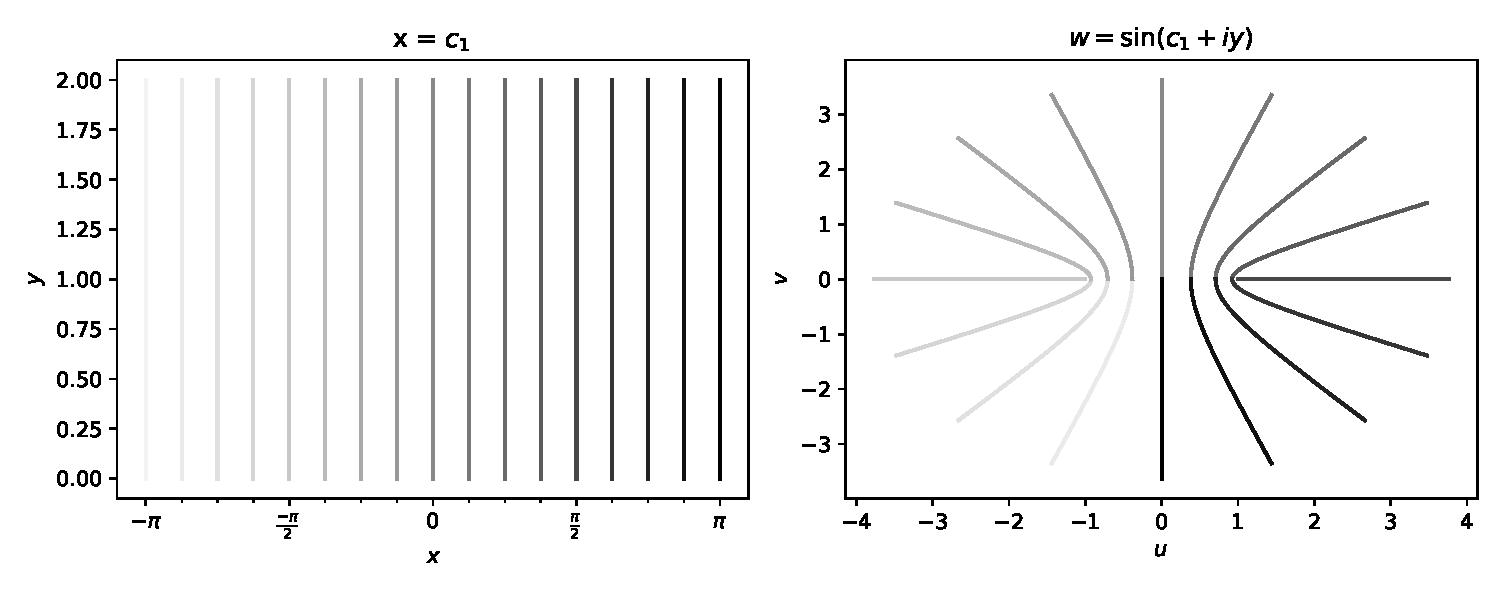
\includegraphics[width=0.9\linewidth]{Python/Mapping_by_Sine_V}
		\label{fig:mappingbysinev}
		\caption*{}
	\end{figure}

%	\subsection{Mappings of the Horizontal Line Segments} \label{Mappings of the Horizontal Line Segments by Sine Subsection - Complex}
	\textbf{Mappings of the Horizontal Line Segments}
	
	As before, we have:
	\begin{align*}
		u &= \sin(x) \cosh(c_2) & v &= \cos(x) \sinh(c_2)
	\end{align*}
	Which gives us the ellipse
	\begin{align*}
		\frac{u^2}{\cosh[2](c_2)} + \frac{v^2}{\sinh[2](c_2)} = 1
	\end{align*}
	with foci
	\begin{align*}
		w = \pm \sqrt{\cosh[2](c_2) - \sinh[2](c_2)} = \pm 1
	\end{align*}

	Since \(u = \sin(x) \cosh(c_2)\) and \(v = \cos(x) \sinh(c_2)\) we can see that as \(x\) increases, the ellipse goes around in a clockwise direction. Since Sine is a cyclic function, we only have 1-1 mappings for constant values of \(y\) in \(x=2\pi\) intervals. Likewise, these 1-1 mappings only hold true for \(y > 0\) or \(y < 0\).
	
	\begin{figure}[H]
		\centering
		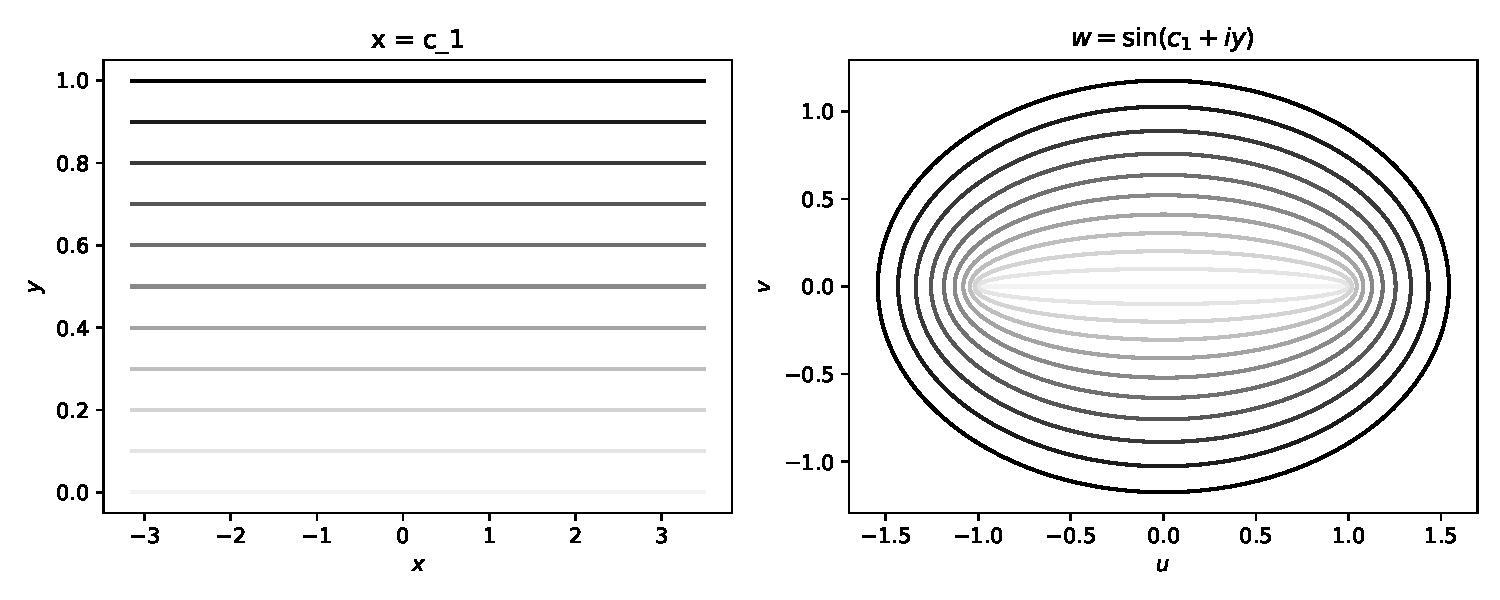
\includegraphics[width=0.9\linewidth]{Python/Mapping_by_Sine_H}
		\caption*{}
		\label{fig:mappingbysineh}
	\end{figure}

	\textbf{Summary}
	
	Basically, the mapping \(w = \sin(z)\) maps vertical line segments to hyperbolas and horizontal line segments to ellipses.

	\begin{example}
		The following rectangular region is mapped onto the semi-elliptical region in a 1-1 manner.
		We have the mapping of the points:
		\begin{align*}
			A = (\pi/2, 0) &\mapsto A' = (1, 0) &
			B = (\pi/2, bi) &\mapsto B' = (\cosh(b), 0) \\
			C = (0, bi) &\mapsto C'=(0, \sinh(b)) &
			D = (-\pi/2, bi) &\mapsto D' = (-\cosh(b), 0) \\
			E = (-\pi/2, 0) &\mapsto E' = (-1, 0) &
			F = (0,0) &\mapsto F' = (0,0)
		\end{align*}
		\begin{figure}[H]
			\centering
			\begin{tikzpicture}[baseline=(current bounding box.center)]
				\begin{axis}[
					unit vector ratio=1 1 1,
					xlabel={$x$},
					ylabel={$y$},
					xmin=-2, xmax=2,
					ymin=-0.2, ymax=2,
					axis lines = middle,
					ticks=none,
					grid=none,
					]
					
					\addplot[
					only marks,
					nodes near coords,
					point meta = explicit symbolic, 
					mark=*,
					]
					coordinates {
						({pi/2}, 0) [\(A\)]
						({pi/2}, 1) [\(B\)]
						(0, 1)		[\(C\)]
						({-pi/2}, 1) [\(D\)]
						({-pi/2}, 0) [\(E\)]
						(0, 0) [\(F\)]
					};
					
					\draw[line width=1pt]
					(axis cs: {pi/2}, 0)--(axis cs: {pi/2}, 1);
					
					\draw[line width=1pt,
					decoration={markings, mark=at position 0.25 with {\arrow{<}} },
					postaction={decorate}]
					(axis cs: {pi/2}, 1)--(axis cs: {-pi/2}, 1);
					
					\draw[line width=1pt]
					(axis cs: {-pi/2}, 1)--(axis cs: {-pi/2}, 0);
					
					\draw[line width=1pt]
					(axis cs: {-pi/2}, 0)--(axis cs: {pi/2}, 0);
				\end{axis}
			\end{tikzpicture}
			{\Large \(\xrightarrow{\mathmakebox[2cm] {f(z)=\sin(z)}}\)}
			\begin{tikzpicture}[baseline=(current bounding box.center)]
				\begin{axis}[
					unit vector ratio=1 1 1,
					xlabel={$u$},
					ylabel={$v$},
					xmin=-10, xmax=10,
					ymin=-0.2, ymax=8,
					axis lines = middle,
					ticks = none,
					grid=none,
					]
					
					\addplot[
					only marks,
					nodes near coords,
					point meta = explicit symbolic, 
					mark=*,
					]
					coordinates {
						(3, 0) [\(A'\)]
						(8, 0) [\(B'\)]
						(0, 5) [\(C'\)]
						(-8, 0) [\(D'\)]
						(-3, 0) [\(E'\)]
						(0, 0) [\(F'\)]
					};
					
					\draw[line width=1pt,]
					(axis cs: 8, 0) -- (axis cs: -8, 0);
					
					\draw[line width=1pt,
					decoration={markings, mark=at position 0.125 with {\arrow{<}} },
					postaction={decorate}]
					(axis cs: 0,0) ellipse (8 and 5);
				\end{axis}
			\end{tikzpicture}
		\end{figure}
	\end{example}
	
	\subsection{Related Mappings} \label{Related Mappings to Sine Subsection - Complex}
	
	\begin{example}
		\index{Mapping! Cosine}
		Consider 
		\begin{align*}
			w = \cos(z) = \sin(z + \frac{\pi}{2})
		\end{align*}
		It is clear the cosine is just the sine function translated to the right by \(\pi / 2\). It is composed of the transformations:
		\begin{align*}
			Z &= z + \frac{\pi}{2} & w = \sin(Z)
		\end{align*}
	\end{example}

	\begin{example}
		\index{Mapping! Hyperbolic Sine}
		Consider
		\begin{align*}
			w = \sinh(z) = -i\sin(iz)
		\end{align*}
		Which is the composite of transformations
		\begin{align*}
			Z &= iz & W &= \sin(Z) & w &= -iW
		\end{align*}
		Hence, it is the sine transformation with rotations by \(\pi/2\) and \(-\pi/2\).
	\end{example}

	\begin{example}
		\index{Mapping! Hyperbolic Cosine}
		Consider
		\begin{align*}
			w = \cosh(z) = \cos(iz)
		\end{align*}
		Which is the a rotation by \(\pi /2 \) followed by a cosine transform.
		Using
		\begin{align*}
			\sin(z + \frac{\pi}{2}) &= \cos(z) & \cos(iz) &= \cosh(z)
		\end{align*}
		We can write \(w = \cosh(z)\):
		\begin{align*}
			w &= \sin(Z) & Z &= iz + \frac{\pi}{2}
		\end{align*}
	\end{example}
	
	\section{Mappings by \texorpdfstring{\(z^2\)}{TEXT}} \label{Mappings by z^2 Section - Complex}
	
	\index{Mapping! \texorpdfstring{\(z^2\)}{TEXT}}
	
	We can write the transformation:
	\begin{align*}
		w &= z^2 = x^2 - y^2 + 2xy = u + iv &
		u &= x^2 - y^2 & 
		v &= 2xy
	\end{align*}

	We can see that if \(x\) is constant, as \(y\) increases, the transformation curves to the left due to the decreasing value of \(u\). It is clear that if we include negative values of \(y\), then the mapping is not 1-1.
	\begin{figure}[H]
		\centering
		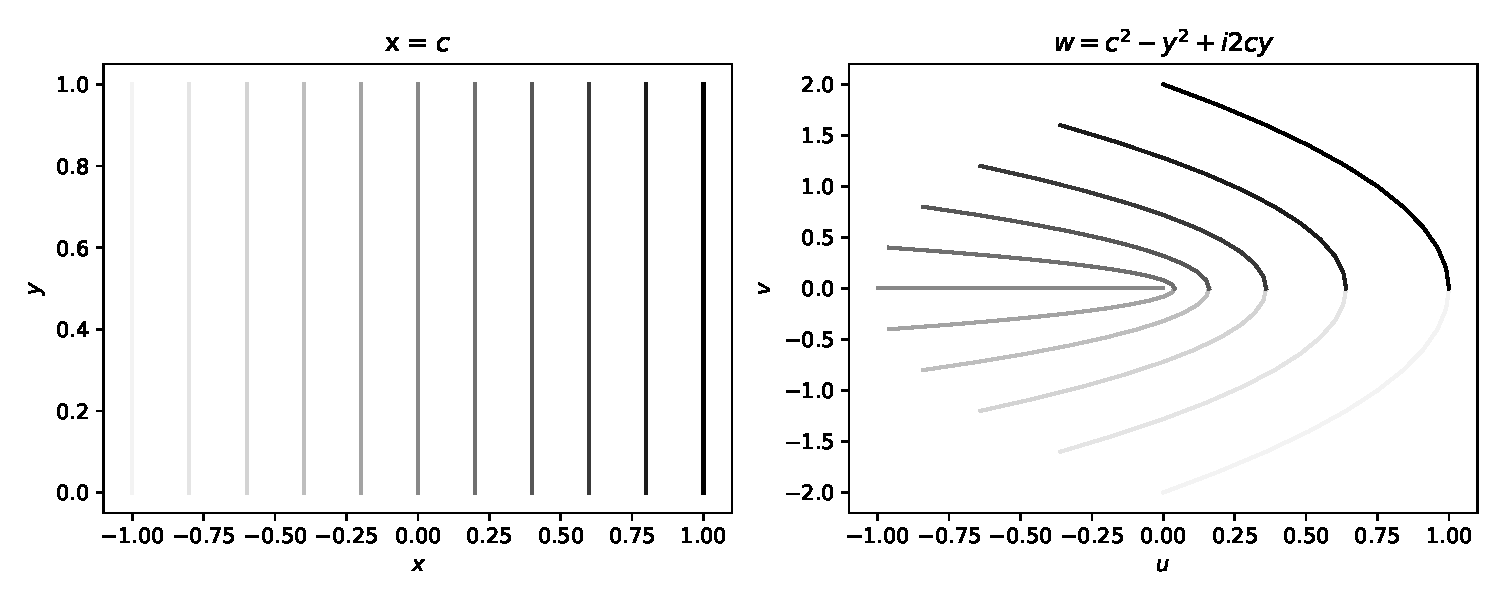
\includegraphics[width=0.9\linewidth]{Python/Mapping_by_z_Squared_V}
		\caption*{}
		\label{fig:mappingbyzsquaredv}
	\end{figure}
	
	If \(y\) is held constant, the increasing value of \(x\) curves the transformation to the right. More accurately, while \(x\) is negative, it moves left until \(x=0\), then it curves to the left due to the parabolic nature of \(u = x^2 - y^2\). The mapping is not 1-1, if we include negative values of \(y\).
	\begin{figure}[H]
		\centering
		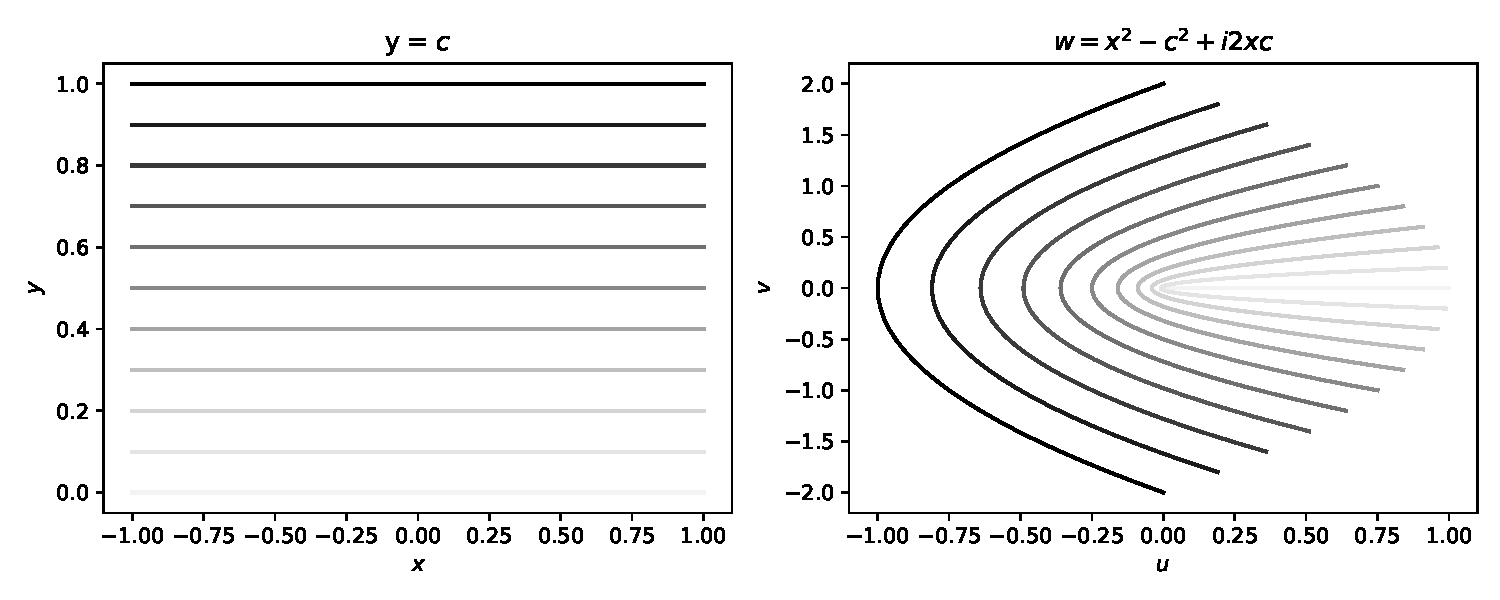
\includegraphics[width=0.9\linewidth]{Python/Mapping_by_z_Squared_H}
		\caption*{}
		\label{fig:mappingbyzsquaredh}
	\end{figure}

	\section{Mappings by Branches of \texorpdfstring{\(z^{1/n}\)}{TEXT}} \label{Mappings by z Square Root Section - Complex}
	
	\index{Mapping! \texorpdfstring{\(z^{1/n}\)}{TEXT}}
	
	Recall \cref{Roots of z Sections - Complex}.
	
	
	\textbf{Square root transformation:} \newline
	For \(z \neq 0\) and in polar coordinates,
	\begin{align*}
		z^{1/2} &= \sqrt{r}e^{i(\Theta + 2\pi x)/2}
			& k \in \mathbb{N}
	\end{align*}
	
	Looking at the Principal Branch, the transformation becomes:
	\begin{align*}
		F_0(z) &= \sqrt{r} e^{i\Theta /2}
			& r>0, \ -\pi < \Theta < \pi
	\end{align*}
	
	It is clear in the principal branch, the mapping is a 1-1 mapping of points in \(-\pi < \Theta < \pi\) to \(-\pi/2 < \Phi < \pi/2\).
	
	When \(\theta = \alpha\) is used to define a branch cut:
	\begin{align*}
		f_\alpha(z) &= \sqrt{r} \exp(\frac{i\theta}{2})	&
			r>0,& \ \alpha < \theta < \alpha + 2\pi
	\end{align*}
	We can extend this to nonzero points on the branch cut by defining \(f_\alpha(0) = 0\), however, such extensions are not continuous on the entire complex plane.
	
	\textbf{\(n\)-th roots of \(z\):}\newline
	\begin{align*}
		z^{1/n} &= \exp(\frac{1}{n} \log(z)) = \sqrt[n]{r} e^{i(\Theta + 2k\pi)/n}
			& n \in \mathbb{N}, \ k \in \{0, 1, 2, \ldots, n-1\}
	\end{align*}
	Then the transformation of each branch \(k\)of \(z^{1/n}\):
	\begin{align*}
		F_k(z) &= \sqrt[n]{r} \exp(\frac{i(\Theta + 2k\pi)}{n})
			& k= \{0, 1, 2, \ldots, n-1\}
	\end{align*}
	It is a 1-1 mapping from the domain:
	\begin{align*}
		r &\mapsto \rho = \sqrt[n]{r} &
		\left[-\pi < \Theta < \pi\right] &\mapsto \left[\frac{(2k-1)\pi}{n} < \phi < \frac{(2k+1)\pi}{n}\right]
	\end{align*}
	
	Likewise, for the principal branch (\(k=0\)), we can construct transformations \(f_\alpha(z)\) branch cuts at \(\theta = \alpha\) as before.
	
	\section{Square Roots of Polynomials} \label{Square Roots of Polynomials Section - Complex}
	
	\begin{example}
		If we consider \(Z^{1/2} = (z - z_0)^{1/2}\):
		\begin{align*}
			Z^{1/2} &= \sqrt{R} \exp(\frac{i\theta}{2})
				& R>0, &\ \alpha < \theta < \alpha + 2\pi
		\end{align*}
		By writing 
		\begin{align*}
			R &= \abs{z-z_0} &
			\Theta &= \operatorname{Arg}(z - z_0) &
			\theta &= \arg(z-z_0)
		\end{align*}
		We have the two branches of \((z-z_0)^{1/2}\):
		\begin{align*}
			G_0(z) &= \sqrt{R} \exp(\frac{i\Theta}{2})	&
				R>0, &\ -\pi < \Theta < \pi \\
			g_0(z) &= \sqrt{R} \exp(\frac{i\theta}{2})	&
				R>0, &\ 0 < \Theta < 2\pi
		\end{align*}
		We can see that for \(w = G_0\), there is a 1-1 mapping:
		\begin{align*}
			\abs{z-z_0} &\mapsto \sqrt{\abs{z-z_0}}
				& \left[-\pi < \operatorname{Arg}(z-z_0) < \pi \right] &\mapsto
					\left[-\frac{\pi}{2} < \frac{\operatorname{Arg}(z-z_0)}{2} < \frac{\pi}{2}\right]
		\end{align*}
		For \(w = g_0(z)\), the 1-1 mapping:
		\begin{align*}
			\abs{z-z_0} &\mapsto \sqrt{\abs{z-z_0}}
				& \left[0 < \arg(z-z_0) < 2\pi \right] &\mapsto
					\left[0 < \frac{\arg(z-z_0)}{2} < \pi \right]
		\end{align*}
	\end{example}

	\begin{example}
		Consider 
		\begin{align*}
			w = (z^2 - 1)^{1/2}
		\end{align*}
		Then we can write
		\begin{align*}
			(z^2 - 1)^{1/2} 
			&= \exp(\frac{1}{2}\log(z^2 - 1)) = \exp(\frac{1}{2}\log(z-1) + \frac{1}{2}\log(z+1)) \\
			&= (z-1)^{1/2} (z+1)^{1/2} & z \neq \pm 1
		\end{align*}
		Note: If \(f_1(z)\) is a branch of \((z-1)^{1/2}\) defined on domain \(D_1\) and \(f_2(z)\) is a branch of \((z+1)^{1/2}\) defined on domain \(D_2\), then \(f(z) = f_1(z) f_2(z)\) is a branch of \((z^2 - 1)^{1/2}\) defined at all points in \(D_1 \cup D_2\).
		
		For branches of \((z-1)^{1/2}\) and \((z-1)^{1/2}\):
		\begin{align*}
			f_1(z) &= \sqrt{r_1} \exp(\frac{i\theta_1}{2})	&
				r_1 &= \abs{z-1} & 
				\theta_1 &= \arg(z-1) &
				r_1>0, &\ \theta_1 \in (0, 2\pi) \\
			f_2(z) &= \sqrt{r_2} \exp(\frac{i\theta_2}{2})	&
				r_2 &= \abs{z+1} & 
				\theta_2 &= \arg(z+1) &
				r_2>0, &\ \theta_2 \in (0, 2\pi)
		\end{align*}
		Then the branch \(f\) of \((z^2 - 1)^{1/2}\):
		\begin{align*}
			f(z) &= \sqrt{r_1 r_2} \exp(\frac{i(\theta_1 + \theta_2)}{2}) &
				r_k > 0, &\ \theta_k \in (0, 2\pi), \ k \in \{1,2\}
		\end{align*}
		
		\begin{figure}[H]
			\centering
			\begin{tikzpicture}
				\begin{axis}[
					unit vector ratio=1 1 1,
					xlabel={$x$},
					ylabel={$y$},
					xmin=-2, xmax=2,
					ymin=-0.2, ymax=2,
					axis lines = middle,
					ticks=none,
					grid=none,
					]
					
					\addplot[
					only marks,
					nodes near coords,
					point meta = explicit symbolic, 
					mark=*,
					]
					coordinates {
						(1.5, 1.75) [\(z\)]
					};
				
					\addplot[
					only marks,
					nodes near coords,
					point meta = explicit symbolic, 
					mark=o,
					]
					coordinates {
						(1, 0) [\(1\)]
						(-1, 0) [\(-1\)]
					};
					
					\draw[]
					(axis cs: 1, 0)--(axis cs: 1.5, 1.75)
					node[pos=0.5, right] {\(r_1\)};
					
					\draw[]
					(axis cs: -1, 0)--(axis cs: 1.5, 1.75)
					node[pos=0.5, above] {\(r_2\)};
					
					\draw[line width=1pt, dashed, color=White]
					(axis cs: -1, 0)--(axis cs: 1.9, 0);
					
					\draw[
					decoration={markings, mark=at position 1 with {\arrow{>}} },
					postaction={decorate}]
					(axis cs: 1.5, 0) arc (0:{atan(1.75/0.5)}:50)
					node[pos=0.5, right] {\(\theta_1\)};
				
					\draw[
					decoration={markings, mark=at position 1 with {\arrow{>}} },
					postaction={decorate}]
					(axis cs: -0.5, 0) arc (0:{atan(1.75/2.5)}:50)
					node[pos=0.5, right] {\(\theta_2\)};
				\end{axis}
			\end{tikzpicture}
		\end{figure}
	
		We can extend this to a function that is analytic everywhere in \(\mathbb{C}\) except \(x \in [-1, 1]\):
		\begin{align*}
			F(z) &= \sqrt{r_1 r_2} \exp(\frac{i(\theta_1 + \theta_2)}{2}) &
				r_k > 0, \ r_1 + r_2 > 2, &\ \theta_k \in (0, 2\pi), \ k \in \{1,2\}
		\end{align*}
	
		We need to show \(F\) is analytic on \(r_1>0\), \(\theta_1 =0\), since \(f(z) = F(z)\) everywhere except there. Consider:
		\begin{align*}
			G(z) &= \sqrt{r_1 r_2} \exp(\frac{i(\Theta_1 \Theta_2)}{2})	&
				r_1 &= \abs{z-1}, \ r_2 = \abs{z+1}, \ \Theta_1 = \operatorname{Arg}(z-1), \Theta_2 = \operatorname{Arg}(z+1) \\
			&&
				r_k &> 0, \ \Theta_k \in (-\pi, \pi), \ k \in \{1,2\}
		\end{align*}
			
		\(G\) analytic in entire \(z\)-plane except for \(r_1 \geq 0\), \(\Theta_1 = \pi\). \(F(z) = G(z)\) when \(r_1 >0\) and \(\Theta_1 \in [0,\pi)\), so \(\theta_k = \Theta_k\). When \(\Theta_1 \in (0, -\pi)\), \(\theta_k = \Theta_k + 2\pi\).
		Then
		\begin{align*}
			\exp(i\theta_k/2) = -\exp(i\Theta_k/2) 
			\implies \exp(\frac{i(\theta_1 + \theta_2)}{2}) = \exp(\frac{i(\Theta_2 + \Theta_2)}{2})
		\end{align*}
		So \(F(z) = G(z)\), in the domain containing \(r_1 > 0\), \(\Theta_1 = 0\), so \(G\) being analytic in the domain implies \(F\) being analytic in the domain. Thus, \(F\) is analytic everywhere except \(x \in [-1, 1]\).
		
		\(F(z)\) cannot be extended to a function analytic at points \(x \in [-1, 1]\), because \(F(z)\) jumps from \(i \sqrt{r_1 r_2}\) to \(-i \sqrt{r_1 r_2}\) as \(z\) moves across the line segment, thus is not continuous.
		
		\(F(z)\) is a 1-1 mapping of \(D_z \mapsto D_w\) except for \(v \in [-1, 1]\).
		\begin{figure}[H]
			\centering
			\begin{tikzpicture}[baseline=(current bounding box.center)]
				\begin{axis}[
					unit vector ratio=1 1 1,
					xlabel={$x$},
					ylabel={$y$},
					xmin=-1.5, xmax=2,
					ymin=-0.2, ymax=2,
					axis lines = middle,
					ticks=none,
					grid=none,
					]
					
					\addplot[
					only marks,
					nodes near coords,
					point meta = explicit symbolic, 
					mark=*,
					]
					coordinates {
						(1.5, 1.75) [\(z\)]
					};
					
					\addplot[
					only marks,
					nodes near coords,
					point meta = explicit symbolic, 
					mark=o,
					]
					coordinates {
						(1, 0) [\(1\)]
						(-1, 0) [\(-1\)]
					};
				
					\addplot[
					only marks,
					nodes near coords,
					point meta = explicit symbolic, 
					mark=none,
					]
					coordinates {
						(-1, 1) [\(D_z\)]
					};
					
					\draw[]
					(axis cs: 1, 0)--(axis cs: 1.5, 1.75)
					node[pos=0.5, right] {\(r_1\)};
					
					\draw[]
					(axis cs: -1, 0)--(axis cs: 1.5, 1.75)
					node[pos=0.5, above] {\(r_2\)};
					
					\draw[line width=1pt, dashed, color=White]
					(axis cs: -1, 0)--(axis cs: 1, 0);
					
					\draw[
					decoration={markings, mark=at position 1 with {\arrow{>}} },
					postaction={decorate}]
					(axis cs: 1.5, 0) arc (0:{atan(1.75/0.5)}:50)
					node[pos=0.5, right] {\(\theta_1\)};
					
					\draw[
					decoration={markings, mark=at position 1 with {\arrow{>}} },
					postaction={decorate}]
					(axis cs: -0.5, 0) arc (0:{atan(1.75/2.5)}:50)
					node[pos=0.5, right] {\(\theta_2\)};
				\end{axis}
			\end{tikzpicture}
			{\Large \(\xrightarrow{\mathmakebox[3cm] {F(z)=(z^2 - 1)^{1/2} }}\)}
			\begin{tikzpicture}[baseline=(current bounding box.center)]
				\begin{axis}[
					unit vector ratio=1 1 1,
					xlabel={$u$},
					ylabel={$v$},
					xmin=-1, xmax=2,
					ymin=-1.5, ymax=2,
					axis lines = middle,
					ticks = none,
					grid=none,
					]
					
					\addplot[
					only marks,
					nodes near coords,
					point meta = explicit symbolic, 
					mark=*,
					]
					coordinates {
						(1.75, 1.75) [\(w\)]
					};
					
					\addplot[
					only marks,
					nodes near coords,
					point meta = explicit symbolic, 
					mark=o,
					]
					coordinates {
						(0, 1) [\(i\)]
						(0,-1) [\(-i\)]
					};
					
					\addplot[
					only marks,
					nodes near coords,
					point meta = explicit symbolic, 
					mark=none,
					]
					coordinates {
						(-0.75, 1) [\(D_w\)]
					};
					
					\draw[]
					(axis cs: 0, 1)--(axis cs: 1.75, 1.75)
					node[pos=0.5, above] {\(\rho_1\)};
					
					\draw[]
					(axis cs: 0,-1)--(axis cs: 1.75, 1.75)
					node[pos=0.5, above] {\(\rho_2\)};
					
					\draw[line width=1pt, dashed, color=White]
					(axis cs: 0, 1)--(axis cs: 0, -1);
					
					\draw[]
					(axis cs: 0, 1)--(axis cs: 0.75, 1);
					
					\draw[]
					(axis cs: 0,-1)--(axis cs: 0.75,-1);
					
					\draw[
					decoration={markings, mark=at position 1 with {\arrow{>}} },
					postaction={decorate}]
					(axis cs: 0.5, 1) arc (0:{atan(0.75/1.75)}:50)
					node[pos=0.5, right] {\(\phi_1\)};
					
					\draw[
					decoration={markings, mark=at position 1 with {\arrow{>}} },
					postaction={decorate}]
					(axis cs: 0.5,-1) arc (0:{atan(2.75/1.75)}:50)
					node[pos=0.5, right] {\(\phi_2\)};
				\end{axis}
			\end{tikzpicture}
		\end{figure}
	
		Note: 
		\begin{align*}
			[z = iy] \land [y>0] \implies [r_1 = r_2 > 1] \land [\theta_1 + \theta_2 = \pi]
		\end{align*}
		Hence the mappings:
		\begin{align*}
			[y>0]\land[x=0] &\mapsto v > 1 & [y<0]\land[x=0] &\mapsto v < -1 \\
			y>0 &\mapsto v>0 &  y<0 &\mapsto v>0 \\
			[r_1>0]\land[\theta_1 = 0] &\mapsto [u>0] \land [v = 0] & 
				[r_2>0] \land [\theta_2 = \pi] &\mapsto [u<0] \land [v = 0]
		\end{align*}
		
		To show \(w = F(z)\) is 1-1:
		\begin{align*}
			F(z_1) = F(z_2) \implies z_1^2 - 1 = z_2^2 - 1 \implies [z_1 = z_2] \lor [z_1 = - z_2]
		\end{align*}
		Since \(F\) maps upper half plane to upper half plane and lower half planes to lower half planes, and the way portions of the real axis in \(D_z\) is mapped, \(z_1 = -z_2\) is impossible, so \(z_1 = z_2\). Thus, \(F(z_1) = F(z_2) \implies F\) is 1-1.
		
		We can show \(F: D_z \mapsto D_w\) by finding \(H: D_w \mapsto D_z\) which \(z = H(w) \implies w = F(z)\). That is, \(H = F^{-1}\). We have
		\begin{align*}
			w = (z^2 - 1)^{1/2} &\implies z = (w^2 + 1)^{1/2} = (w - i)^{1/2} (w-i)^{1/2}
				& w \neq \pm i
		\end{align*}
		Writing 
		\begin{align*}
			w - i &= \rho_1 e^{i\phi_1} & w + i &= \rho_2 e^{i\phi_2} &
				\rho_k > 0, \ \rho_1 + \rho_2 > 2, \ \phi_k \in \left[-\frac{\pi}{2}, \frac{3\pi}{2}\right], \ k \in \{1,2\}
		\end{align*}
		Hence
		\begin{align*}
			H(w) &= \sqrt{\rho_1 \rho_2} \exp(\frac{i(\phi_1 + \phi_2)}{2})	&
				\text{Domain: } D_w
		\end{align*}
		with mappings:
		\begin{align*}
			v > 0 &\mapsto y > 0 & v < 0 \mapsto y<0 \\
			[u>0] \land [y=0] &\mapsto [x>1] \land [y=0] & 
				[u<0] \land [y=0] &\mapsto [x< -1] \land [y=0] 
		\end{align*}
		Then 
		\begin{align*}
			z = H(w) 
			&\implies z^2 = w^2 + 1 \implies w^2 = z^2 -1
		\end{align*}
		Since \(z \in D_z\) and \(w = \pm (z^2 - 1)^{1/2}\), we have \(w = F(z)\) and \(w = -F(z)\). By \(H(w)\) mapping upper half plane to upper half plane and lower half planes to lower half planes, and the mapping of segments of the real axis in the domains, we have \(w = F(z)\).
	\end{example}
	
	For mappings by branches of double-valued functions:
	\begin{align*}
		w &= (z^2 + Az + B)^{1/2} = [(z-z_0)^2 - z_1^2]^{1/2} &
			A &= -2z_0 & B = z_0^2 = z_1^2 &
			z_1 \neq 0
	\end{align*}
	We can use methods in the above example on the successive transformations:
	\begin{align*}
		Z &= \frac{z-z_0}{z_1} &
		W &= (Z^2 - 1)^{1/2} &
		w &= z_1 W
	\end{align*}
	
	
	\section{Riemann Surface} \label{Riemann Surface} \index{Riemann Surface}
	
	\begin{definition}[Riemann Surface (Informal Definition)]
		\label{Riemann Surface Informal Definition - Complex}
		\index{Riemann Surface}
		A generalized complex plane with more than one ``sheet''. It's a one dimensional complex manifold.
	\end{definition}
	
	On a Riemann surface, a multi-valued function is assigned a single-value. As such, the theory of single-valued function applies.
	
	\begin{example}
		Consider the multi-valued function:
		\begin{align*}
			\log(z) = \ln(r) + i\theta
		\end{align*}
		The Riemann surface of \(\log(z)\) is then the complex plane with a deleted origin, and a cut made along the positive real axis. The first sheet \(R_0\) is defined from \(\theta \in [0, 2\pi]\), the second sheet \(R_1\) consists of \(\theta \in [2\pi, 4\pi]\), the third sheet \(R_3\) consists of \(\theta \in [4\pi, 6\pi]\), and so on. Likewise, the sheet \(R_{-1}\) consists of \(\theta \in [-2\pi, 0]\). 
		
		Essentially, we get an infinite ``spiral staircase'' with sheets in multiples of \(2\pi\). The radial component, of course, is also infinite.
		
		\begin{figure}[H]
			\centering
			\begin{tikzpicture}
				\begin{axis}[
					axis equal,
					width=10cm,
					axis lines = center,
					xlabel = {$x$},
					ylabel = {$y$},
					zlabel = {$\theta$},
					xmin=-2, xmax=2,
					ymin=-2, ymax=2,
					zmin=-2.5, zmax=2.5,
					ticks = none,
					axis lines = middle,
					axis line style = Black,
					%				enlargelimits=0.3,
					view/h=45,
					scale uniformly strategy=units only,
					]
					
					\addplot3[patch,
						patch refines=1,
						shader=faceted interp,
						opacity = 0.2,
						domain = -4*pi:4*pi,
						domain y = 0:1,
						samples = 101,
						samples y = 2,
						]
						({y*cos(deg(x))},
						{y*sin(deg(x))},
						{deg(x)}/360);
					
					\draw[dashed] (axis cs: 0,0,2) -- (axis cs: 1.9,0,2);
					\draw[dashed] (axis cs: 0,0,1) -- (axis cs: 1.9,0,1);
					\draw[dashed, color=White] (axis cs: 0,0,0) -- (axis cs: 1.9,0,0);
					\draw[dashed] (axis cs: 0,0,-1) -- (axis cs: 1.9,0,-1);
					\draw[dashed] (axis cs: 0,0,-2) -- (axis cs: 1.9,0,-2);
				\end{axis}
			\end{tikzpicture}
		\end{figure}
	
		The transformation \(w = \log(z)\) maps the Riemann surface onto the \(w\)-plane in an 1-1 manner. 
		
		\begin{figure}[H]
			\centering
			\begin{tikzpicture}[baseline=(current bounding box.center)]
				\begin{axis}[
					axis equal,
					width=10cm,
					axis lines = center,
					xlabel = {$x$},
					ylabel = {$y$},
					zlabel = {$\theta$},
					xmin=-2, xmax=2,
					ymin=-2, ymax=2,
					zmin=-2.5, zmax=2.5,
					ticks = none,
					axis lines = middle,
					axis line style = Black,
					%				enlargelimits=0.3,
					view/h=45,
					scale uniformly strategy=units only,
					]
					
					\addplot3[patch,
					patch refines=1,
					shader=faceted interp,
					opacity = 0.2,
					domain = -4*pi:4*pi,
					domain y = 0:1,
					samples = 101,
					samples y = 2,
					]
					({y*cos(deg(x))},
					{y*sin(deg(x))},
					{deg(x)}/360);
					
					\draw[dashed] (axis cs: 0,0,2) -- (axis cs: 1.9,0,2);
					\draw[dashed] (axis cs: 0,0,1) -- (axis cs: 1.9,0,1);
					\draw[dashed, color=White] (axis cs: 0,0,0) -- (axis cs: 1.9,0,0);
					\draw[dashed] (axis cs: 0,0,-1) -- (axis cs: 1.9,0,-1);
					\draw[dashed] (axis cs: 0,0,-2) -- (axis cs: 1.9,0,-2);
				\end{axis}
			\end{tikzpicture}
			{\Large \(\xrightarrow{\mathmakebox[3cm] {F(z)=\log(z) }}\)}
			\begin{tikzpicture}[baseline=(current bounding box.center)]
				\begin{axis}[
					unit vector ratio=1 1 1,
					xlabel={$u$},
					ylabel={$v$},
					xmin=-3, xmax=3,
					ymin=-2.5, ymax=3,
					axis lines = middle,
					ticks = none,
					grid=none,
					]
					
					\addplot[
					only marks,
					nodes near coords,
					point meta = explicit symbolic, 
					mark=*,
					]
					coordinates {
						(0, 2) [\(4\pi i\)]
						(0, 1) [\(2\pi i\)]
						(0,-1) [\(-2\pi i\)]
						(0,-2) [\(-4\pi i\)]
					};
					
					
					\draw[dashed]
					(axis cs: -3, 2)--(axis cs: 3, 2);
					
					\draw[dashed]
					(axis cs: -3, 1)--(axis cs: 3, 1);
					
					\draw[dashed]
					(axis cs: -3,-1)--(axis cs: 3,-1);
					
					\draw[dashed]
					(axis cs: -3,-2)--(axis cs: 3,-2);
				\end{axis}
			\end{tikzpicture}
		\end{figure}
		\(\log(z)\) on \(R_1\) is an analytic continuation of \(f(z) = \ln(r) + i\theta\), \(\theta \in (0, 2\pi)\). \(\log(z)\) is then not only single-valued on all points \(z\) on the Riemann surface, but also analytic at all points. 
		
		The ``spiral staircase'' can be cut along any ray from the origin to for other Riemann surfaces.
	\end{example}

	\begin{example}
		Consider the square root function on the \(z\)-plane with a deleted origin:
		\begin{align*}
			z^2 = \sqrt{r}e^{i\theta/2}
		\end{align*}
		The function maps \(\theta \in [0, 2\pi]\) to \(\phi \in [0, \pi]\), and \(\theta \in [2\pi, 4\pi]\) to \(\phi \in [\pi, 2\pi]\). Thus the Riemann surface is composed of two sheets, \(R_1\) and \(R_2\).
		
		\begin{figure}[H]
			\centering
			\begin{tikzpicture}
				\begin{axis}[
					axis equal,
					width=10cm,
					axis lines = center,
					xlabel = {$x$},
					ylabel = {$y$},
					zlabel = {$\theta$},
					xmin=-2, xmax=2,
					ymin=-2, ymax=2,
					zmin=-2, zmax=2,
					ticks = none,
					axis lines = middle,
					axis line style = Black,
					%				enlargelimits=0.3,
					view/h=45,
					scale uniformly strategy=units only,
					]
					
					\addplot3[patch,
					patch refines=1,
					shader=faceted interp,
					opacity = 0.2,
					domain = -4*pi:4*pi,
					domain y = 0:1,
					samples = 101,
					samples y = 2,
					]
					({y*cos(deg(x))},
					{y*sin(deg(x))},
					{y*sin(deg(x/2))});
					
					
					\draw[dashed, color=White] (axis cs: 0,0,0) -- (axis cs: 1.9,0,0);
				\end{axis}
			\end{tikzpicture}
		\end{figure}
	
		The function is now single-valued. The choice of values of \(\theta\) from \(0\) to \(2\pi\) or \(4\pi\) to \(6\pi\) does not affect the value of \(z^{1/2}\). Note, the value of \(z^{1/2}\) a point where the sheet passes from \(R_0\) to \(R_1\) is different than that passing from \(R_1\) to \(R_0\). \(R_0\) for \(\theta \in (0, 2\pi)\), and \(R_1\) for \(\theta \in (2\pi, 4\pi)\).
		
		The origin is common to both \(R_0\) and \(R_1\), thus is a branch point of the Riemann Surface.
		
		The function is an analytic continuation of the function defined on the other sheet, thus points of \(z^{1/2}\) on the Riemann surface are all analytic except at the origin.
	\end{example}

	
	\subsection{Surfaces for Related Functions} \label{Surfaces for Related Functions Subsection - Complex}
	
	\begin{example}
		Riemann surface for
		\begin{align*}
			f(z) = (z^2 - 1)^{1/2} &= \sqrt{r_1 r_2} \exp(\frac{i(\theta_1 + \theta_2)}{2}) &
			z - 1 &= r_1 e^{i\theta_1} &
			z + 1 &= r_2 e^{i\theta_2}
		\end{align*}
		\begin{figure}[H]
			\centering
			\begin{tikzpicture}
				\begin{axis}[
					unit vector ratio=1 1 1,
					xlabel={$x$},
					ylabel={$y$},
					xmin=-2, xmax=2,
					ymin=-0.2, ymax=2,
					axis lines = middle,
					ticks=none,
					grid=none,
					]
					
					\addplot[
					only marks,
					nodes near coords,
					point meta = explicit symbolic, 
					mark=*,
					]
					coordinates {
						(1.5, 1.75) [\(z\)]
					};
					
					\addplot[
					only marks,
					nodes near coords,
					point meta = explicit symbolic, 
					mark=o,
					]
					coordinates {
						(1, 0) [\(1\)]
						(-1, 0) [\(-1\)]
					};
					
					\draw[]
					(axis cs: 1, 0)--(axis cs: 1.5, 1.75)
					node[pos=0.5, right] {\(r_1\)};
					
					\draw[]
					(axis cs: -1, 0)--(axis cs: 1.5, 1.75)
					node[pos=0.5, above] {\(r_2\)};
					
					\draw[line width=1pt, dashed, color=White]
					(axis cs: -1, 0)--(axis cs: 1.9, 0);
					
					\draw[
					decoration={markings, mark=at position 1 with {\arrow{>}} },
					postaction={decorate}]
					(axis cs: 1.5, 0) arc (0:{atan(1.75/0.5)}:50)
					node[pos=0.5, right] {\(\theta_1\)};
					
					\draw[
					decoration={markings, mark=at position 1 with {\arrow{>}} },
					postaction={decorate}]
					(axis cs: -0.5, 0) arc (0:{atan(1.75/2.5)}:50)
					node[pos=0.5, right] {\(\theta_2\)};
				\end{axis}
			\end{tikzpicture}
		\end{figure}
	
		We have a branch cut between the points \(z = \pm 1\), thus the Riemann surface has two sheets cut between the points. The lower edge of \(R_0\) is connected to the upper edge of \(R_1\), and lower edge of \(R_1\) is connected to the upper edge of \(R_0\). We have two layers where the line between \(z=\pm 1\) serves as a connection between the layers.
		
		Any simple closed curve enclosing \(z = \pm 1\) on a sheet will return to its original position as \(\theta_1\) and \(\theta_2\) go from \(0\) to \(2\pi\), and will not cross into the other sheet. 
		
		If a contour encircles \(z = 1\) twice, but does not enclose \(z=-1\), then the contour passes from \(R_0\) to \(R_1\) and back to \(R_0\). \(\theta_1\) then changes by \(4\pi\) while \(\theta_2\) changes by \(0\). Likewise for a similar case enclosing \(z = -1\).
		
	\end{example}
	
	\begin{example}
		Consider the double-valued function:
		\begin{align*}
			f(z) = [z(z^2 - 1)]^{1/2} = \sqrt{r r_1 r_2} \exp(\frac{i(\theta + \theta_1 + \theta_2)}{2})
		\end{align*}
		\begin{figure}[H]
			\centering
			\begin{tikzpicture}
				\begin{axis}[
					unit vector ratio=1 1 1,
					xlabel={$x$},
					ylabel={$y$},
					xmin=-2, xmax=2,
					ymin=-0.5, ymax=2,
					axis lines = middle,
					ticks=none,
					grid=none,
					]
					
					\addplot[
					only marks,
					nodes near coords,
					point meta = explicit symbolic, 
					mark=*,
					]
					coordinates {
						(1.5, 1.75) [\(z\)]
					};
					
					\addplot[
					only marks,
					nodes near coords,
					point meta = explicit symbolic, 
					mark=o,
					]
					coordinates {
						(1, 0) [\(1\)]
						(0, 0)
						(-1, 0) [\(-1\)]
					};
					
					\draw[]
					(axis cs: 1, 0)--(axis cs: 1.5, 1.75)
					node[pos=0.5, right] {\(r_1\)};
					
					\draw[]
					(axis cs: -1, 0)--(axis cs: 1.5, 1.75)
					node[pos=0.5, above] {\(r_2\)};
					
					\draw[]
					(axis cs: 0, 0)--(axis cs: 1.5, 1.75)
					node[pos=0.5, above] {\(r\)};
					
					\draw[line width=1pt, dashed, color=White]
					(axis cs: -1, 0)--(axis cs: 0, 0)
					node[pos=0.5, below, color=Black] {\(L_1\)};
					
					\draw[line width=1pt, dashed, color=White]
					(axis cs: 1, 0)--(axis cs: 1.9, 0)
					node[pos=0.5, below, color=Black] {\(L_2\)};
					
					\draw[
					decoration={markings, mark=at position 1 with {\arrow{>}} },
					postaction={decorate}]
					(axis cs: 1.5, 0) arc (0:{atan(1.75/0.5)}:50)
					node[pos=0.5, right] {\(\theta_1\)};
					
					\draw[
					decoration={markings, mark=at position 1 with {\arrow{>}} },
					postaction={decorate}]
					(axis cs: -0.5, 0) arc (0:{atan(1.75/2.5)}:50)
					node[pos=0.5, right] {\(\theta_2\)};
					
					\draw[
					decoration={markings, mark=at position 1 with {\arrow{>}} },
					postaction={decorate}]
					(axis cs: 0.5, 0) arc (0:{atan(1.75/1.5)}:50)
					node[pos=0.5, right] {\(\theta\)};
				\end{axis}
			\end{tikzpicture}
		\end{figure}
		The branch points are \(z \in \{0, \pm 1\}\). Since the function is double-valued, we will have two sheets, \(R_0\) and \(R_1\). We can define a cut \(L_1\) from \(-1\) to \(0\) and a cut \(L_2\) from \(1\) to a point at infinity. The sheets \(R_0\) and \(R_1\) is then joined along \(L_1\) and \(L_2\), with the lower edge of \(R_0\) joined to the upper edge of \(R_1\) and the lower edge of \(R_1\) joined to the lower edge of \(R_0\).
		\begin{question}
			Is the choice of the cuts \(L_1\) and \(L_2\) arbitrary? Can we define \(L_1\) as the point at infinity to \(-1\) and \(L_2\) from \(0\) to \(1\)?
		\end{question}
	\end{example}

	\chapter{Conformal Mapping} \label{Conformal Mapping Chapter - Complex}
	
	\index{Conformal Mapping}
	
	A map that locally conforms to the original shape of a region.

	\section{Preserving Angles and Scale Factors} \label{Preserning Angles and Scale Factors}
	
	\begin{definition}[Conformal]
		\index{Conformal}
		\label{Conformal Definition - Complex}
		A transformation \(w = f(z)\) is conformal at point \(z_0\) if \(f\) is analytic at \(z_0\) and \(f'(z_0) \neq 0 \). That is, the orientation and magnitude of the angles between curves are preserved.
		\begin{align*}
			[f \text{ analytic at } z_0] \land [f'(z_0) \neq 0]
			\implies f \text{ Conformal}
		\end{align*}
	\end{definition}
	
	Consider an arc \(C_1\) parameterized by \(z_1(t)\) and a function \(f\) defined by all points in \(C\):
	\begin{align*}
		z_1 &= z_1(t) & 
		w_1 &= f[z_1(t)] &
		t &\in [a, b] 
	\end{align*}
	Thus \(w\) is the parametric representation of image \(\Gamma_1\) of \(C_1\). Suppose there exists \(z_0 = z_1(t_0) \in (a, b)\) such that \(f\) is analytic and \(f'(z_0) \neq 0\). Then
	\begin{align*}
		w_1'(t_0) = f'[z_1(t_0)] z_1'(t_0) 
		&\implies \arg[w_1'(t_0)] = \arg[f'[z_1(t_0)]] + \arg[z_1'(t_0)] \\
		&\implies \arg[f'[z_1(t_0)]] = \arg[w_1'(t_0)] - \arg[z_1'(t_0)]
	\end{align*}
	Hence, we can see that \(w'(t_0)\) and \(z'(t_0)\) differs by an angle of rotation \(\varphi_0 = \arg[f'(z_0)]\).
	
	\begin{definition}[Angle of Rotation]
		\index{Angle of Rotation}
		\label{Angle of Rotation Definition - Complex}
		Let \(z_0 = z(t_0)\) be a point in an arc \(C\), and \(w = f(z)\) be a conformal transformation. Then the angle of rotation is the difference between the angle of \(C\) at \(z_0\) and its image \(\Gamma\) under \(w\) at \(f(z_0)\).
	\end{definition}
	
	If we consider another arc \(C_2\) passing through \(z_0 = z_2(t_0)\) with image \(\Gamma_2\) under the same transformation \(w\). We obtain:
	\begin{align*}
		\arg[w_2'(t_0)] &= \arg[f'[z_2(t_0)]] + \arg[z_2'(t_0)] & \text{For } C_2 \\
		\arg[w_1'(t_0)] &= \arg[f'[z_1(t_0)]] + \arg[z_1'(t_0)]  & \text{For } C_1
	\end{align*}
	Since we have \(z_1(t_0) = z_2(t_0) = z_0\), if we subtract the two, we have 
	\begin{align*}
		\arg[w_1'(t_0)] - \arg[w_2'(t_0)] = \arg[z_1'(t_0)] - \arg[z_2'(t_0)]
	\end{align*}
	Hence, the angle between \(C_1\) and \(C_2\) at \(z_0\) is the same as the angle between \(\Gamma_1\) and \(\Gamma_2\) at \(f(z_0)\). The angles between the curves at \(z_0\) and orientation of the angles are preserved in the transformation.
	
	\begin{figure}[H]
		\centering
		\begin{tikzpicture}[baseline=(current bounding box.center)]
			\begin{axis}[
				unit vector ratio=1 1 1,
				xlabel={$x$},
				ylabel={$y$},
				xmin=-0.2, xmax=10,
				ymin=-0.2, ymax=10,
				axis lines = middle,
				ticks=none,
				grid=none,
				]
				
				\draw[line width=1pt, color=Blue, 
				decoration={markings, mark=at position 0.8 with {\arrow{>}} },
				postaction={decorate}]
				(axis cs: 1, 5)--(axis cs: 9, 5)
				node[pos=0.8, below] {\(C_1\)};
				
				\draw[line width=1pt, color=Red,
				decoration={markings, mark=at position 0.8 with {\arrow{>}} },
				postaction={decorate}]
				(axis cs: 5, 1)--(axis cs: 5, 9) 
				node[pos=0.8, right] {\(C_2\)};
				
				\draw[decoration={markings, mark=at position 1 with {\arrow{>}} },
				postaction={decorate}]
				(axis cs: 6, 5) arc (0:90:10)
				node[pos=0.5, right] {\(\varphi_0\)};
			\end{axis}
		\end{tikzpicture}
		{\Large \(\xrightarrow{\mathmakebox[2cm]{w = f(z)}}\)}
		\begin{tikzpicture}[baseline=(current bounding box.center)]
			\begin{axis}[
				unit vector ratio=1 1 1,
				xlabel={$u$},
				ylabel={$v$},
				xmin=-0.2, xmax=10,
				ymin=-0.2, ymax=10,
				axis lines = middle,
				ticks = none,
				grid=none,
				]
				
				\draw[line width=1pt, color=Blue, 
				decoration={markings, mark=at position 0.9 with {\arrow{>}} },
				postaction={decorate}]
				(axis cs: 1, 1) -- (axis cs: 6, 8)
				node[pos=0.9, right] {\(\Gamma_1\)};
				
				\draw[line width=1pt, color=Red,
				decoration={markings, mark=at position 0.9 with {\arrow{>}} },
				postaction={decorate}]
				(axis cs: {6*cos(20)}, {6*sin(20)}) arc (20:80:60)
				node[pos=0.9, below] {\(\Gamma_2\)};
				
				\draw[decoration={markings, mark=at position 1 with {\arrow{>}} },
				postaction={decorate}]
				(axis cs: {7*cos(atan(8/6))}, {7*sin(atan(8/6))}) 
				arc ({atan(8/6)}:{atan(8/6) + 90}:10)
				node[pos=0.5, above] {\(\varphi_0\)};
				
				\draw[dashed]
				(axis cs: {6*cos(atan(8/6))}, {6*sin(atan(8/6))}) 
				-- (axis cs: {6*cos(atan(8/6)) - 4*0.75}, {6*sin(atan(8/6)) + 3*0.75});
			\end{axis}
		\end{tikzpicture}
	\end{figure}
	
	From \cref{f nequiv 0 in some neighbourhood of z_0 implies f neq 0 in some deleted neighbourhood of z_0 Theorem - Complex} we can see that \(w\) is also conformal in some neighbourhood of \(z_0\). If this applies to an entire domain:
	
	\begin{definition}[Conformal Mapping/Transformation]
		\index{Conformal Mapping} \index{Conformal Transformation}
		\label{Conformal Mapping Definition - Complex}
		A transformation \(w = f(z)\) is conformal if \(\forall z \in D\), \(f(z)\) is analytic and \(f'(z) \neq 0\).
		\begin{align*}
			\forall z \in D [f \text{ analytic } \land f(z) \neq 0] 
			\implies f \text{ Conformal Mapping}
		\end{align*}
	\end{definition}

	\begin{example}
		Consider two smooth arcs that are level curves of 
		\begin{align*}
			f(z) = u(x,y) + iv(x,y) 
		\end{align*}
		Suppose \(u(x,y) = c_1\) and \(v(x,y) = c_2\) intersect at point \(z_0\), where \(f\) is analytic and nonzero at \(z_0\). Then \(f\) must be conformal at \(z_0\). If the two curves are orthogonal at \(z_0\) then they are orthogonal at \(w_0 = f(z_0)\).
	\end{example}

	\begin{definition}[Isogonal Mapping]
		\index{Isogonal Mapping}
		\label{Isogonal Mapping Definition - Complex}
		A mapping that preserves the angle between two curves, but not the orientation of the angle.
	\end{definition}
	
	\begin{example}
		Consider the transformation 
		\[w = \bar{z}\]
		It is isogonal, not conformal, due to \(w = \bar{z}\) not being an analytic function. If followed by an conformal map \(f\), the result \(w = f(\bar{z})\) is isognal. That is, \textbf{conformal transformations preserves isogonal transformations}.
	\end{example}
	
	\begin{definition}[Critical Point]
		\index{Critical Point}
		\label{Critical Point Definition - Complex}
		A function \(f\) that is non-constant and analytic at \(z_0\), and \(f(z_0) = 0\). Then \(z_0\) is a critical point of transformation \(w = f(z)\).
	\end{definition}

	\begin{example}
		Consider 
		\begin{align*}
			w = 1 + z^2
		\end{align*}
		Which is a composition of mappings
		\begin{align*}
			Z &= z^2	&	w = 1 + Z
		\end{align*}
		\(z_0 = 0\) is a critical point of \(w\). We can see that \(z_0 = 0 \mapsto w_0 = 1\), and that \(w\) doubles any angle at \(z_0\). 
	\end{example}

	\begin{corollary}
		Suppose \(z_0\) is a critical point of \(w = f(z)\). Let \(\Gamma_1\) and \(\Gamma_2\) be the image of curves \(C_1\) and \(C_2\) under the transformation respectively. If the angle between \(C_1\) and \(C_2\) at \(z_0\) is \(\alpha\), then the angle between \(\Gamma_1\) and \(\Gamma_2\) at \(w_0 = f(z_0)\) becomes \(m \alpha\) under \(w\) for \(m \geq 2\), \(m \in \mathbb{N}\). Also, \(m\) is the smallest natural number such that \(f^{(m)}(z_0) \neq 0\). 
		
		That is, if \(z_0\) is a critical point of \(w = f(z)\), then angles between curves \(\alpha\) at \(z_0\) becomes \(m\alpha\) under \(f(z)\) for \(m \geq 2\), \(m \in \mathbb{N}\), and \(f(z)\) has a zero of order \(m\) at \(z_0\).
	\end{corollary}
	\begin{proof}
		\Cref{Zero of order m and critical point Example - Complex}
	\end{proof}
	
	\begin{definition}[Scale Factor]
		\index{Scale Factor}
		\label{Scale Factor Definition - Complex}
		The Scale Factor, \(\abs{f'(z_0)}\), is the amount of scaling inflicted on the distances under the transformation \(w = f(z)\). Consider the modulus of the derivative of the transformation \(w = f(z)\):
		\begin{align*}
			\abs{f'(z_0)}
			= \abs{\lim_{z \rightarrow z_0} \frac{f(z) - f(z_0)}{z - z_0}}
			= \lim_{z \rightarrow z_0} \frac{\abs{f(z) - f(z_0)}}{\abs{z - z_0}}
		\end{align*}
		For any \(z\) close to \(z_0\):
		\begin{align*}
			\abs{f'(z_0)} \approx \frac{\abs{f(z) - f(z_0)}}{\abs{z - z_0}}
		\end{align*}
		which represents the ratio between the distances \(f(z) - f(z_0)\) and \(z - z_0\) under the transformation.
	\end{definition}
	
	It is clear that \(\abs{f'(z_0)} > 1\) represents an expansion while \(\abs{f'(z_0) < 1}\) represents a contraction.
	
	From the continuity of \(f'(z)\) we see that for \(z\) close to \(z_0\):
	\begin{align*}
		\arg[f'(z)] &\approx \arg[f'(z_0)] & \abs{f'(z)} &\approx \abs{f'(z_0)}
	\end{align*}
	Hence, the image of a conformal transformation approximates that of the original neighbourhood locally. That is, it is \textit{conforms} to the shape of the original region. Notice, it is \textit{locally} not \textit{globally}.
	
	\begin{example}
		Consider 
		\begin{align*}
			f(z) = z^2 = x^2 - y^2 + i2xy
			\implies f'(z) = 2z
		\end{align*}
		The function is entire and \(f'(z)\) is zero only at the origin. Consider the half lines 
		\begin{align*}
			y &= x & x &= 1 & x, y \geq 0
		\end{align*}
		which is denoted as the curves \(C_1\) and \(C_2\) that intersect at \(z_0 = 1 + i\). It is clear that the angle between the curves are \(\pi / 4\). 
		
		Under the transformation, \(C_1 \mapsto \Gamma_1\), with \(\Gamma_1\) parameterization:
		\begin{align*}
			u &= 0 & v &= 2x & 0 \leq x < \infty
		\end{align*}
		\(C_2 \mapsto \Gamma_2\), with \(\Gamma_2\) parameterization:
		\begin{align*}
			u &= 1 - y^2 & v &= 2y & 0 \leq y < \infty
		\end{align*}
		\begin{figure}[H]
			\centering
			\begin{tikzpicture}[baseline=(current bounding box.center)]
				\begin{axis}[
					unit vector ratio=1 1 1,
					xlabel={$x$},
					ylabel={$y$},
					xmin=-0.2, xmax=5,
					ymin=-0.2, ymax=5,
					axis lines = middle,
					ticks=none,
					grid=none,
					]
					
					\addplot[
					only marks,
					nodes near coords,
					point meta = explicit symbolic, 
					mark=*,
					]
					coordinates {
						(1, 1) [\(1 + i\)]
					};
					
					\draw[line width=1pt, color=Blue, 
					decoration={markings, mark=at position 0.8 with {\arrow{>}} },
					postaction={decorate}]
					(axis cs: 0, 0)--(axis cs: 4, 4)
					node[pos=0.8, left] {\(C_1\)};
					
					\draw[line width=1pt, color=Red,
					decoration={markings, mark=at position 0.8 with {\arrow{>}} },
					postaction={decorate}]
					(axis cs: 1, 0)--(axis cs: 1, 4) 
					node[pos=0.8, left] {\(C_2\)};
					
					\draw[decoration={markings, mark=at position 1 with {\arrow{>}} },
					postaction={decorate}]
					(axis cs: 2, 2) arc (45:90:{(2^0.5)*100})
					node[pos=0.5, above] {\(\frac{\pi}{4}\)};
				\end{axis}
			\end{tikzpicture}
			{\Large \(\xrightarrow{\mathmakebox[2cm]{f(z)= z^2} }\)}
			\begin{tikzpicture}[baseline=(current bounding box.center)]
				\begin{axis}[
					unit vector ratio=1 1 1,
					xlabel={$u$},
					ylabel={$v$},
					xmin=-4, xmax=2,
					ymin=-0.2, ymax=5,
					axis lines = middle,
					ticks = none,
					grid=none,
					]
					
					\addplot[
					only marks,
					nodes near coords,
					point meta = explicit symbolic, 
					mark=*,
					]
					coordinates {
						(1, 0) [\(1\)]
						(0, 2) [\(2i\)]
					};
					
					\draw[line width=1pt, color=Blue, 
					decoration={markings, mark=at position 0.9 with {\arrow{>}} },
					postaction={decorate}]
					(axis cs: 0, 0) -- (axis cs: 0, 4)
					node[pos=0.9, right] {\(\Gamma_1\)};
					
					\addplot [
						domain=0:2, 
						samples=100, 
						color=Red,
						line width=1pt,
						postaction = {decorate, 
							decoration={markings, mark=at position 0.9 with {\arrow{>};} }}
						]
						({1-x^2}, {2*x})
						node[pos=0.9, below] {\(\Gamma_2\)};
					
					\draw[decoration={markings, mark=at position 1 with {\arrow{>}} },
					postaction={decorate}]
					(axis cs: 0, 3) arc (90:135:100)
					node[pos=0.5, above] {\(\frac{\pi}{4}\)};
					
					\draw[dashed]
					(axis cs: 0, 2) -- (axis cs: -2, 4);
				\end{axis}
			\end{tikzpicture}
		\end{figure}
		
		We then have
		\begin{align*}
			\dv{v}{u} = \frac{\dv*{v}{y}}{\dv*{u}{y}} = \frac{2}{-2y} = - \frac{2}{v}
		\end{align*}
		\(v = 2 \implies \dv*{v}{u} = -1\), so the angle between \(\Gamma_1\) and \(\Gamma_2\) at \(w = f(1+i) = 2i\) is \(\pi/4\). Hence, we have conformality of the mapping.
	
		The angle of rotation:
		\begin{align*}
			\arg[f'(1+i)] &= \arg[2(1+i)] = \frac{\pi}{4} + 2n \pi	&
				n \in \mathbb{Z}
		\end{align*}
		Scale factor:
		\begin{align*}
			\abs{f'(1+i)} = \abs{2(1+i)} = 2\sqrt{2}
		\end{align*}
	\end{example}
	
	\section{Local Inverses} \label{Local Inverses Section - Complex}
	
	\begin{definition}[Local Inverse]
		\index{Local Inverse}
		\label{Local Inverse Definition - Complex}
		Suppose a transformation \(w = f(z)\) be conformal and \(w_0 = f(z_0)\). Then a local inverse of the transformation is a unique transformation \(z = g(w)\) defined and analytic in a neighbourhood \(N\) of \(w_0\) such that \(\forall w \in N\), \(g(w_0) = z_0\) and \(f[g(w)] = w\). The derivative:
		\begin{align*}
			g'(w) = \frac{1}{f'(w)}
		\end{align*}
	\end{definition}
	\begin{proof}
		{\color{Grey}
		Prove: 
		\begin{align*}
			g'(w) = \frac{1}{f'(w)}
		\end{align*}
		Let \(w = f[g(w)]\), then 
		\begin{align*}
			\dv{w} w = \dv{w} f[g(w)]
			&\implies 1 = f'[g(w)] g'(w) 
			 \implies g'(w) = \frac{1}{f'(w)}
		\end{align*}}
	\end{proof}
	Note: From the definition, \(z = g(w)\) is conformal at \(w_0\).
	
	\textbf{Existence of the Inverse:} \newline
	Conformality of the transformation \(w = f(z)\) at \(z_0\) implies there exist a neighbourhood of \(z_0\) that \(f\) is analytic. Hence
	\begin{align*}
		f(z) &= u(x,y) + iv(x,y) &
		z &= x + iy &
		z_0 &= x_0 + iy_0
	\end{align*}
	Then there exists some neighbourhood of \(x_0, y_0\) where \(u\) and \(v\) and their partial derivatives of all orders are continuous (\cref{Analytic implies existance of high order derivatives theorem - Complex}). The Jacobian is then nonzero at \(z_0\):
	\begin{align*}
		\operatorname{J} 
		&= \mdet{u_x & u_y \\ v_x & v_y} = u_x v_y - v_x u_y 
	 	 = (u_x)^2 + (v_x)^2 & u_x = v_y, \ u_y = -v_x \\
		&= \abs{f'(z)}^2 \neq 0 
			& \text{Conformal at } z_0, \ \text{\Cref{Cauchy-Riemann Differentiablity Conditions Theorem - Complex}}
	\end{align*}
	The condition on the Jacobian and derivatives of \(u\) and \(v\) are sufficient conditions to ensure invertibility of transform. So, if 
	\begin{align*}
		u_0 &= u(x_0, y_0) & v_0 = v(x_0, y_0)
	\end{align*}
	then there exists a unique continuous transformation
	\begin{align*}
		x &= x(u,v) & y &= y(u,v)
	\end{align*}
	that \((u_0, v_0) \mapsto (x_0, y_0)\) in the neighbourhood \(N\). In addition, the first order partial derivatives throughout \(N\) satisfy
	\begin{align*}
		x_u &= \frac{v_y}{\operatorname{J}} &
		x_v &= -\frac{u_y}{\operatorname{J}} &
		y_u &= - \frac{v_x}{\operatorname{J}} &
		y_v &= \frac{u_x}{\operatorname{J}}
	\end{align*}
	which shows that \(g(w)\) is analytic in \(N\).
	\begin{proof}
		{\color{Grey}
		Proving \(g(w)\) is analytic in \(N\):\newline
		We know that \(f(z)\) is analytic, so it satisfies the Cauchy-Riemann equations (\cref{Cauchy-Riemann Equations (Cartesian) Theorem - Complex}). Hence, we can write the above four equations as:
		\begin{align*}
			x_u &= \frac{u_x}{\operatorname{J}} &
			x_v &= -\frac{u_y}{\operatorname{J}} &
			y_u &= \frac{u_y}{\operatorname{J}} &
			y_v &= \frac{u_x}{\operatorname{J}}
		\end{align*}
		It is then clear that 
		\begin{align*}
			x_u &= y_v & x_v &= -v_u
		\end{align*}
		Which are the Cauchy-Riemann equations. Thus \(g(w)\) is analytic in \(N\).
		}
	\end{proof}
	Letting \(z = x + iy\) and \(w = u + iv\):
	\begin{align*}
		z &= g(w) = x(u, v) + iy(u,v) \\
		w &= f(z) = u(x, y) + iv(x,y)
	\end{align*}
	Thus the inverse exists.
	
	\begin{example}
		\label{Zero of order m and critical point Example - Complex}
		{\color{Grey}
		Suppose that \(f\) has a zero of order \(m \in \mathbb{N}\) at \(z_0\), that is 
		\begin{align*}
			f'(z_0) &= f''(z_0) = \cdots = f^{(m-1)}(z_0)	&
				f^{(m)} &\neq 0
		\end{align*}
		Let \(w_0 = f(z_0)\). Using the Taylor expansion of \(f(z)\) about \(z_0\) (\cref{Taylor's Theorem - Complex}):
		\begin{align*}
			f(z) 
			&= \sum_{n=0}^{\infty} \frac{f^{(n)}(z_0)}{n!} (z - z_0)^n
			 = f(z_0) + \sum_{n=m}^{\infty} \frac{f^{(n)}(z_0)}{n!} (z - z_0)^n \\
			&= f(z_0) + \frac{f^{(m)}(z_0)}{m!}(z-z_0)^m + \sum_{n=m+1}^{\infty} \frac{f^{(n)}(z_0)}{n!} (z - z_0)^n \\
		\end{align*}
		This implies that 
		\begin{align*}
			f(z) - f(z_0) = f(z) - w_0
			&= \frac{f^{(m)}(z_0)}{m!} (z - z_0)^m \left[
				1 + \sum_{n=m+1}^{\infty} \frac{f^{(n)}(z_0)}{f^{(m)}(z_0)} \cdot \frac{m!}{n!} (z-z_0)^{n-m}
				\right]\\
			&= \frac{f^{(m)}(z_0)}{m!} (z - z_0)^m [1 + g(z)]
		\end{align*}
		We can see that in \(g(z)\), \(n > m\), so it is a Taylor series which is analytic at \(z_0\). Also, \(g(z_0) = 0\). Let \(C_1\) be a curve with image \(\Gamma_1\) under the transformation \(f\), and \(\theta_0\) be the angle of inclination of \(C_1\) at \(z_0\). Likewise with \(\phi_0\) for \(\Gamma_1\). Then we have 
		\begin{align*}
			\theta_0 &= \lim_{z \rightarrow z_0} \arg(z-z_0) &
			\phi_0 &= \lim_{z \rightarrow z_0} \arg[f(z) - w_0]
		\end{align*}
		Using the results obtained previously:
		\begin{align*}
			\phi_0 
			&= \lim_{z \rightarrow z_0} \arg 
				\left[\frac{f^{(m)}(z_0)}{m!} (z - z_0)^m [1 + g(z)] \right] \\
			&= \lim_{z \rightarrow z_0} \left[m \arg(z-z_0) + \arg [f^{(m)}(z_0)] + \arg\left(\frac{1 + g(z)}{m!}\right) \right]
		\end{align*}
		Since
		\begin{align*}
			&\lim_{z \rightarrow z_0}\frac{1 + g(z)}{m!} 
			 = \frac{1 + g(z_0)}{m!} = \frac{1}{m!} \in \mathbb{R}
			  \implies \arg\left[\frac{1}{m}\right] = 0&
				g(z_0) &= 0
		\end{align*}
		we have
		\begin{align*}
			\phi_0 
			&= \lim_{z \rightarrow z_0} [m \arg(z-z_0)] + \arg[f^{(m)}(z_0)] 
			 = m\theta_0 + \arg[f^{(m)}(z_0)] 
		\end{align*}	
		Now, let another curve \(C_2\) intersect \(C_1\) at \(z_0\), and \(\Gamma_2\) intersect \(\Gamma_1\) at \(w_0\). Then the angle of inclination of \(\Gamma_2\) at \(w_0\): 
		\begin{align*}
			\phi_1 = m \theta_1 + \arg[f^{(m)}(z_0)]
		\end{align*}
		Let \(\alpha\) be the angle between \(C_1\) and \(C_2\) at \(z_0\). Since we are still under the transformation \(f\), the angle between \(\Gamma_1\) and \(\Gamma_2\) at \(w_0\):
		\begin{align*}
			\phi_1 - \phi_0 
			&= m(\theta_1 - \theta_0) + \arg[f^{(m)}(z_0)] - \arg[f^{(m)}(z_0)]  = m\alpha
				& \alpha = \theta_1 - \theta_0
		\end{align*}
		If the mapping is conformal, \(\phi_1 - \phi_0 = \theta_1 - \theta_0 = \alpha\), so \(m = 1\).
		
		Note: Since \(f\) has a zero of order \(m\), \(f'(z_0) = 0\) for all \(m \geq 2\), so \(z_0\) is a critical point of \(f\) for \(m \geq 2\) by \cref{Critical Point Definition - Complex}. Thus the transformed angle is an natural number multiple of the original angle at a critical point.
		}
	\end{example}
	
	\section{Harmonic Conjugates} \label{Harmonic Conjugates Section - Complex}
	\index{Function! Harmonic! Conjugate} \index{Harmonic Function! Conjugate}
	\index{Harmonic Conjugate}
	
	Review \cref{Harmonic Functions Section - Complex}.
	
	Recall from the definition of a Harmonic Conjugate (\cref{Harmonic Conjugate Definition - Complex}). If function \(f(z) = u(x,y) + iv(x,y)\) is analytic in a domain \(D\), then \(v(x,y)\) is a harmonic conjugate of \(u(x,y)\). \newline
	
	\begin{theorem}
		\label{Analytic Implies v harmonic conjugate of u Theorem - Complex}
		Let \(f(z) = u(x,y) + iv(x,y)\) be a function in domain \(D\).
		\begin{align*}
			f \text{ analytic in } D \iff v \text{ is harmonic conjugate of } u
		\end{align*}
	\end{theorem}
	\begin{proof}
		\underline{\(\impliedby\)}: \newline
		\begin{align*}
			&v \text{ is harmonic conjugate of } u \\
			&\implies \text{Cauchy-Riemann Equations Satisfied} \\
			&\implies f \text{ analytic in } D & \text{\Cref{Cauchy-Riemann Differentiablity Conditions Theorem - Complex}}
		\end{align*}
		\underline{\(\implies\)}: \newline
		\begin{align*}
			&f \text{ analytic in } D \\
			&\implies u \text{ and } v \text{ harmonic } 
				& \text{\Cref{Analytic implies Harmonic Theorem - Complex}} \\
			&\implies \text{Cauchy-Riemann Equations satisfied} 
				& \text{\Cref{Cauchy-Riemann Equations (Cartesian) Theorem - Complex}}
		\end{align*}
	\end{proof}
	
	\begin{example}[\(v\) harmonic conjugate of \(u\) does \textbf{not imply} \(u\) harmonic conjugate of \(v\)]
		Consider 
		\begin{align*}
			u(x,y) &= x^2 - y^2 & v(x,y) &= 2xy
		\end{align*}
		We know that \(v\) is a harmonic conjugate of \(u\) since \(f(z) = x^2 - y^2 + i2xy = z^2\) is entire. However, \(u\) is not a harmonic conjugate of \(v\), since \(g(z) = 2xy + i(x^2 - y^2)\) does not satisfy the Cauchy-Riemann equations and are not analytic anywhere:
		\begin{align*}
			u_x &= 2y & v_y &= -2y \\
			u_y &= 2x & -v_x &= -2x
		\end{align*}
	\end{example}

	\begin{example}(Finding Harmonic Conjugates)
		Consider 
		\begin{align*}
			u(x,y) &= 2x(1-y)
		\end{align*}
		By Cauchy-Riemann equation, we have \(u_x = v_y = 2-2y\). By integrating:
		\begin{align*}
			v(x,y) &= 2y - y^2 + g(x)
		\end{align*}
		By \(u_y = -v_x = -2x \implies g_x = 2x\), then
		\begin{align*}
			v(x,y) &= 2y - y^2 + x^2 + C
		\end{align*}
		Therefore
		\begin{align*}
			f(z) = 2x(1-y) + i(2y - y^2 + x^2 + C) = 2z + i(z^2 + C)
		\end{align*}
		It is customary to write \(C=0\), since \(C\) is arbitrary, so
		\begin{align*}
			f(z) = 2z + iz^2
		\end{align*}
	\end{example}

	\begin{theorem}
		\label{Harmonic Function on Simply Connected Domain always have harmonic conjugate v Theorem - Complex}
		Let \(f(z) = u(x,y) + iv(x,y)\) be a harmonic function in a simply connected domain \(D\), then \(u\) has a harmonic conjugate \(v\) in \(D\).
	\end{theorem}
	\begin{proof}
		Supposes \(P(x,y)\) and \(Q(x,y)\) have continuous first-order partial derivatives in simply connected domain \(D\). If \(P_y = Q_x\) everywhere in \(D\), then the integral over contour \(C\) from \((x_0,y_0)\) to \((x,y)\):
		\begin{align*}
			\int_{C} P(s,t) ds + Q(s,t) dt
		\end{align*}
		is path independent in \(D\). If \((x_0, y_0)\) is fixed, then 
		\begin{align*}
			F(x,y) = \int_{(x_0, y_0)}^{(x,y)} P(s, t) ds + Q(s,t) dt
		\end{align*}
		is single-valued, with first-order partial derivatives:
		\begin{align*}
			F_x(x,y) &= P(x,y) &
			F_y(x,y) &= Q(x,y)
		\end{align*}
		It follows from Laplace's Equation, that everywhere in \(D\):
		\begin{align*}
			u_{xx} + u_{yy} = 0
			\implies (-u_y)_y = (u_x)_x
		\end{align*}
		Since the second-order partial derivatives of \(v\) are continuous in \(D\), the first-order partial derivatives are continuous in \(D\) as well. Then for a fixed \((x_0, y_0) \in D\):
		\begin{align*}
			v(x,y) = \int_{(x_0, y_0)}^{(x,y)} - u_t(s,t) ds + u_s(s,t) dt
		\end{align*}
		is well defined \(\forall (x,y) \in D\). Therefore 
		\begin{align*}
			&[F_x(x,y) = P(x,y)] \land [F_y(x,y) = Q(x,y)] \\
			&\implies [v_x(x,y) = -u_y(x,y)] \land [v_y (x,y) = u_x(x,y)]
		\end{align*}
		Hence, the first-order partial derivatives of \(u\) are also continuous in \(D\). Thus \(u(x,y) + iv(x,y)\) is analytic in \(D\) and \(v\) is a harmonic conjugate of \(u\).
		
		Note: \(v\) is not the only harmonic conjugate of \(u\), since the conditions for a harmonic conjugate is satisfied by a family of functions \(v(x,y) + C\) for all \(C \in \mathbb{R}\).
	\end{proof}
	
	\begin{example}
		{\color{Grey}
		Consider \(u(r, \theta) = \ln(r)\), we can see that it satisfies the polar form of Laplace's equation:
		\begin{align*}
			r^2 u_{rr}(r, \theta) + ru_r(r, \theta) + u_{\theta \theta}(r,\theta) 
			&= r^2 (-r^{-2}) + r(r^{-1}) = 0
		\end{align*}
		Hence it is harmonic in domain \(r>0\), \(\theta \in (0,2\pi)\). By the polar form of the Cauchy-Riemann equations (\cref{Cauchy-Riemann Equations (Polar) Theorem - Complex}):
		\begin{align*}
			r u_r &= v_\theta = 1 & u_\theta = -rv_r = 0
		\end{align*}
		We can integrate and obtain:
		\begin{align*}
			v(r,\theta) &= \theta + C & C \in \mathbb{R}
		\end{align*}
		Hence the analytic function is
		\begin{align*}
			f(r, \theta) = \ln(r) + i(\theta + C)
		\end{align*}
		}	
	\end{example}
	
	\subsection{Transformation of Harmonic Functions} \label{Transformation of Harmonic Functions Subsection - Complex}
	\index{Harmonic Function! Transformations}
	\index{Transformation! Harmonic Function}
	
	\begin{theorem}
		\label{Harmonic Function Transformed by Analytic Function is Harmonic Theorem - Complex}
		\index{Harmonic Function! Transformed by Analytic Function}
		Let \(f(z): D_z \mapsto D_w\) be an analytic function \(w = f(z) = u(x,y) + iv(x,y)\).
		\begin{align*}
			h(u, v) \text{ harmonic in } D_w
			\implies H(x,y) = h[u(x,y), v(x,y)] \text{ harmonic in } D_z
		\end{align*}
		That is, a transformation of an harmonic function by an analytic function is harmonic. 
		
		(For a more general case of \(h(u,v)\) and alternate proof of the theorem, see \cref{Harmonic Function Transformed by Analytic Function is Harmonic Theorem Alternate Proof Example - Complex}.)
		
		(For the case where \(h(u,v)\) satisfies Poisson's Equation, see \cref{Poisson's Equation Transformed by Analytic Function Example - Complex}.)
	\end{theorem}
	\begin{proof}
		\textbf{\underline{\(D_w\) is simply connected:}} \newline
		\(h(u,v)\) is harmonic in \(D_w\) \(\implies\) \(h(u,v)\) has harmonic conjugate \(g(u,v)\) (\cref{Harmonic Function on Simply Connected Domain always have harmonic conjugate v Theorem - Complex}). Hence, we have function 
		\begin{align*}
			\Phi(w) &= h(u,v) + ig(u,v) &
			\text{Analytic in } D_w
		\end{align*}
		\(f(z)\) is analytic in \(D_w\) \(\implies\) \(\phi[f(z)]\) is analytic in \(D_z\). Hence, \(u(x,y)\) is harmonic in \(H[u(x,y), v(x,y)]\).
		
		\textbf{\underline{\(D_w\) is not simply connected:}} \newline
		\(\forall w_0 \in D_w\), \(w_0\) has a neighbourhood \(\abs{w-w_0}<\epsilon\) lying entirely in \(D_w\). The neighbourhood is simply connected, we have a function:
		\begin{align*}
			\Phi(w) &= h(u,v) + ig(u,v) &
			\text{Analytic in } D_w
		\end{align*}
		\(f\) is continuous at \(z_0 \in D_z \implies \forall \epsilon, \exists \delta > 0 [\abs{w - w_0}< \epsilon \implies \abs{z-z_0} < \delta] \). Hence \(\Phi[f(z)]\) is analytic in neighbourhood \(\abs{z-z_0} < \delta\), so \(h[u(x,y), v(x,y)]\) is analytic in the neighbourhood. Since \(\forall z_0 \in D_w\), \(z_0 \mapsto w_0 \in D_w\) by function \(w = f(z)\), \(h[u(x,y), v(x,y)]\) is harmonic in \(D_z\).
	\end{proof}

	\begin{example}
		Consider
		\begin{align*}
			w = e^z = e^x \cos(y) + ie^x \sin(y)
		\end{align*}
		Which maps \(y \in (0,\pi)\) to \(v>0\). \(w^2\) is analytic in the upper-half plane, so the function 
		\begin{align*}
			h(u,v) = \Re{w^2} = u^2 - v^2
		\end{align*}
		is harmonic in the upper-half plane. By the theorem:
		\begin{align*}
			H(x,y) 
			= (e^x \cos(y))^2 - (e^x \sin(y))^2 
			= e^{2x} [\cos[2](y) - sin[2](y)] 
			= e^{2x} \cos(2y)
		\end{align*}
		is harmonic throughout \(y \in (0,\pi)\).
	\end{example}
	
	\subsection{Transformation of Boundary Conditions} \label{Transformation of Boundary Conditions Subsection - Complex}
	
	\index{Transformation! Boundary Condition}
	
	This theorem allows us to transform complex problems in the \(z\)-plane into simpler problems in the \(w\)-plane, solve it there, and transform back.
	
	\begin{theorem}
		\label{Transformation of Boundary Conditions Theorem - Complex}
		Suppose 
		\begin{itemize}
			\item[1.] \(w = f(z) = u(x,y) + iv(x,y)\) is conformal \(\forall z \in C\) and \(\Gamma = \operatorname{Img}_f(C)\).
			\item[2.] \(h(u,v)\) satisfies 
				\begin{align*}
					\forall w \in \Gamma 
					\left[(h = h_0) \lor \left(\dv{h}{n} = 0\right)\right]
				\end{align*}
				where \(h_0 \in \mathbb{R}\) and \(\dv*{h}{n}\) is the directional derivative of \(h\) normal to \(\Gamma\).
		\end{itemize}
		Then
		\begin{align*}
			H(x,y) &= h[u(x,y), v(x,y)]
		\end{align*}
		satisfies
		\begin{align*}
			\forall z \in C 
			\left[(H = h_0) \lor \left(\dv{H}{N} = 0\right)\right]
		\end{align*}
		where \(\dv*{H}{N}\) is the directional derivative of \(H\) normal to \(C\).
	\end{theorem}
	\begin{proof}
		\underline{\textbf{\(h = h_0\) on \(\Gamma\) \(\implies\) \(H=h_0\) on \(C\):}} 
		\begin{align*}
			H(x,y) = h[u(x,y), v(x,y)] = h_0
		\end{align*}
		
		\underline{\textbf{\(\dv*{h}{n} = 0\) on \(\Gamma \implies \) \(\dv*{H}{N} = 0\) on \(C\):}}
		\begin{align*}
			\dv{h}{n} = \grad{h} \cdot \vec{n}
		\end{align*}
		\(\vec{n}\) is unit vector normal to \(\Gamma\) at \((u,v)\). 
		\begin{align*}
			\eval{\dv{h}{n}}_{(u,v)} = 0
			&\implies \grad{h} \text{ orthogonal to } \vec{n} \text{ at } (u,v) \\
			&\implies \grad{h} \text{ tangent to } \Gamma \text{ at } (u,v) \\
			&\implies \Gamma \text{ orthogonal to } h(u,v) = c
		\end{align*}
		Now
		\begin{align*}
			H(x,y) = c
			\implies h[u(x,y), v(x,y)] = c
		\end{align*}
		\(C \mapsto \Gamma\) and \(\Gamma\) orthogonal to \(h(x,y) = c\) implies \(C\) orthogonal to \(H(x,y) = c\) by conformality of transform. Thus \(\grad{H}\) is tangent to \(C\) at \((x,y)\).
		
		If \(\vec{N}\) is unit vector normal to \(C\) at \((x,y)\), then \(\grad{H}\) is orthogonal to \(N\):
		\begin{align*}
			\grad{H} \cdot \vec{N} = 0
			\implies \dv{H}{N} = \grad{H}\cdot \vec{N} = 0
		\end{align*}
	\end{proof}
	
	The proof assumed \(\grad{h} = 0\). If \(\grad{h} = 0\), then 
	\begin{align*}
		\abs{\grad{H (x,y)}} = \abs{\grad{h(u,v)}} \abs{f'(z)} = 0 
		\implies \grad{h(u,v)} = 0
	\end{align*}
	We also assumed \(\grad{h}\) and \(\grad{H}\) exists and \(H(x,y) = c\) is smooth when \(\grad{h} \neq 0\) at \((u,v)\), which ensures angles are preserved by \(w = f(z)\).
	
	\begin{example}
		Consider \(h(u,v) = v + 2\), with transformation 
		\begin{align*}
			w = iz^2 = i(x + iy)^2 = -2xy + i(x^2 - y^2)
		\end{align*}
		which is conformal for \(z \neq 0\). We have \(h = 2\) for \(x = y\) \((x > 0)\), and \(h_u = 0\). Then 
		\begin{align*}
			H(x,y) = x^2 - y^2 + 2
		\end{align*}
		satisfies \(H = 2\) for \(x = y\) \((x > 0)\) and \(H_y = 0\) for \(x > 0\) by the theorem.
		
		\begin{figure}[H]
			\centering
			\begin{tikzpicture}[baseline=(current bounding box.center)]
				\begin{axis}[
					unit vector ratio=1 1 1,
					xlabel={$x$},
					ylabel={$y$},
					xmin=-0.2, xmax=10,
					ymin=-0.2, ymax=10,
					axis lines = middle,
					ticks=none,
					grid=none,
					]
					
					\draw[line width=1pt, color=Blue, 
					decoration={markings, mark=at position 0.8 with {\arrow{>}} },
					postaction={decorate}]
					(axis cs: 0, 0)--(axis cs: 9, 9)
					node[pos=0.5, right] {\(H = 2\)};
					
					\draw[line width=1pt, color=Red,
					decoration={markings, mark=at position 0.8 with {\arrow{>}} },
					postaction={decorate}]
					(axis cs: 0, 0)--(axis cs: 9, 0) 
					node[pos=0.5, above] {\(H_y = 0\)};
				\end{axis}
			\end{tikzpicture}
			{\Large \(\xrightarrow{\mathmakebox[2cm]{w = f(z)}}\)}
			\begin{tikzpicture}[baseline=(current bounding box.center)]
				\begin{axis}[
					unit vector ratio=1 1 1,
					xlabel={$u$},
					ylabel={$v$},
					xmin=-10, xmax=1,
					ymin=-0.2, ymax=10,
					axis lines = middle,
					ticks = none,
					grid=none,
					]
					
					\draw[line width=1pt, color=Red, 
					decoration={markings, mark=at position 0.9 with {\arrow{>}} },
					postaction={decorate}]
					(axis cs: 0, 0) -- (axis cs: 0, 9)
					node[pos=0.5, left] {\(h_u = 0\)};
					
					\draw[line width=1pt, color=Blue,
					decoration={markings, mark=at position 0.9 with {\arrow{>}} },
					postaction={decorate}]
					(axis cs: 0, 0) -- (axis cs: -9, 0)
					node[pos=0.5, above] {\(h = 2\)};
				\end{axis}
			\end{tikzpicture}
		\end{figure}
	\end{example}
	
	Under a conformal transformation, the ratio of the directional derivative of \(H\) along a smooth arc \(C\) in the \(z\)-plane to the directional derivative of \(h\) along the image \(\Gamma\) in the \(w\)-plane is \(\abs{f'(z)}\).
	
	\begin{example}
		The transformation \(w = f(z) = z^2\) which maps the positive \(x\) and \(y\) axis and the origin in the \(z\) plane onto the \(u\) axis in the \(w\) plane. Consider the harmonic function: 
		\begin{align*}
			h(u,v) = \Re{e^{-w}} = e^{-u} \cos(v)
		\end{align*}
		The normal derivative \(h_v = 0\) along the \(u\) axis. Show the normal derivative of \(H(x,y)\) is zero along both positive axis is the \(z\) plane. Note: \(w = z^2\) is not conformal at the origin.
		\begin{proof}
			{\color{Grey}
			\begin{align*}
				w = z^2 = x^2 - y^2 + i2xy 
				\implies H(x,y) = e^{-x^2 + y^2} \cos(2xy)
			\end{align*}
			Taking the gradient:
			\begin{align*}
				\grad{H} 
				&= e^{-x^2 + y^2} 
				\left\{ [(-2x)\cos(2xy) - (2y)\sin(2xy)]\hat{x} 
				+ [(2y)\cos(2xy) - (2x)\sin(2xy)] \hat{y} \right\} \\
				&= 2 e^{-x^2 + y^2} 
				\left\{ [(-x)\cos(2xy) - (y)\sin(2xy)]\hat{x} 
				+ [(y)\cos(2xy) - (x)\sin(2xy)] \hat{y} \right\}
			\end{align*}
			Taking the normal derivative along \((x,0)\):
			\begin{align*}
				\dv{h}{x} 
				= \grad{H} \cdot \hat{y} 
				= (y)\cos(2xy) - (x)\sin(2xy)
				\implies \grad{H}(x,0) \cdot \hat{y} = 0
			\end{align*}
			Taking the normal derivative along \((0,y)\):
			\begin{align*}
				\dv{h}{x} 
				= \grad{H} \cdot \hat{x} 
				= (-x)\cos(2xy) - (y)\sin(2xy)
				\implies \grad{H}(0, y) \cdot \hat{y} = 0
			\end{align*}
			Hence, the normal derivative of \(H(x,y)\) along both positives axes in the \(z\) plane is zero.
			}
		\end{proof}
	\end{example}

	\begin{example}
		Let \(h(u,v) = \Re{-2iw + e^{-w}} = 2v + e^{-u} \cos(v)\) with the transformation \(w = f(z) = z^2\). Show \(h_v = 2\) along the \(u\) axis, but \(H_y = 4x\) along the positive \(x\) axis and \(H_x = 4y\) along the positive \(y\) axis. Then this illustrates:
		\begin{align*}
			\dv{h}{n} = h_0 \neq 0 \text{ not neccessarily transformed to } 
			\dv{H}{N} = h_0
		\end{align*}
		\begin{proof}
			{\color{Grey}
			Applying the transformation to \(h(u,v)\):
			\begin{align*}
				H(x,y) =  4xy + e^{-x^2 + y^2} \cos(2xy)
			\end{align*}
			For \(h_v\) along the \(u\) axis:
			\begin{align*}
				h_v = 2 - e^{-u} \sin(v) \implies h_v(u, 0) = 2 - e^{-u} \sin(0) = 2
			\end{align*}
			For the partial derivatives of \(H\):
			\begin{align*}
				H_y &= 4x + 2y e^{-x^2 + y^2} \cos(2xy) - e^{-x^2 + y^2} (2x) \sin(2xy) \\
				H_x &= 4y + (-2x) e^{-x^2 + y^2} \cos(2xy) - e^{-x^2 + y^2} (2y) \sin(2xy)
			\end{align*}
			Hence, \(H_y\) along the positive \(x\) axis and \(H_x\) along the positive \(y\) axis:
			\begin{align*}
				H_y (x>0, 0) &= 4x &
				H_x (0, y>0) &= 4y
			\end{align*}
			The statement is proven because despite \(f(z) = z^2\) mapping the positive \(x\) and \(y\) axis in the \(z\) plane to the positive \(u\) axis in the \(w\) plane, the value of the normal derivatives is not preserved in the transformation. That is:
			\begin{align*}
				\dv{H}{y} = H_y = 4x &\neq h_v = 2 &
				\dv{H}{x} = H_x = 4y &\neq h_v = 2
			\end{align*}
			}
		\end{proof}
	\end{example}

	\begin{example}
		\label{Harmonic Function Transformed by Analytic Function is Harmonic Theorem Alternate Proof Example - Complex}
		Suppose an analytic function \(w = f(z) = u(x,y) + iv(x,y)\) maps \(D_z \mapsto D_w\). Let \(h(u,v)\) have continuous first and second order partial derivatives defined on \(D_w\). Show
		\begin{align*}
			H(x,y) = h[u(x,y), v(x,y)] 
			\implies H_{xx}(x,y) + H_{yy}(x,y) = [h_{uu}(u,v) + h_{vv}(u,v)] \abs{f'(z)}^2
		\end{align*}
		\begin{proof}
			{\color{Grey}
			Calculating \(H_x\):
			\begin{align*}
				H_x = h_u u_x + h_v v_x
			\end{align*}
			Calculating the second order partials:
			\begin{align*}
				H_{xx} 
				&= h_{uu} u_x^2 + h_u u_{xx} + h_{uv} u_x v_x + h_{vv} v_x^2 + h_v v_{xx} + h_{vu} u_x v_x \\
				H_{yy}
				&= h_{uu} u_y^2 + h_u u_{yy} + h_{uv} u_y v_y + h_{vv} v_y^2 + h_v v_{yy} + h_{vu} u_y v_y
			\end{align*}
			\(h(u,v)\) have continuous first and second order partial derivatives, so \(h_{uv} = h{vu}\). Since \(f(z)\) is analytic, \(u\) and \(v\) satisfy the Cauchy-Riemann equations (\cref{Cauchy-Riemann Equations (Cartesian) Theorem - Complex}) and Laplace's equation (\cref{Laplace's Equation Definition - Complex}). Therefore, \(u_x = v_y\), \(u_y = -v_x\), \(u_{xx} + u_{yy} = 0\), and \(v_{xx} + v_{yy} = 0\), and we have
			\begin{align*}
				&H_{xx} + H_{yy} \\
				&= h_{uu} (u_x^2 + u_y^2) + h_u (u_{xx} + u_{yy}) + 2h_{uv} (u_x v_x + u_y v_y) + h_{vv} (v_x^2 + v_y^2) + h_v (v_{xx} + v_{yy}) \\
				&= h_{uu} (u_x^2 + v_x^2) + h_{vv} (u_x^2 + v_y^2) + 2h_{uv}(u_x v_x - v_x u_y) \\
				&= (h_{uu} + h_{vv})(u_x^2 + v_x^2)
			\end{align*}
			Since
			\begin{align*}
				\abs{f'(z)}^2 = \abs{u_x + iv_x}^2 = u_x^2 + v_x^2
			\end{align*}
			Hence
			\begin{align*}
				H_{xx} + H_{yy} = [h_{uu} + h_{vv}] \abs{f'(z)}^2
			\end{align*}
			By extension, this tells us that in the nontrivial case where \(\abs{f'(z)} \neq 0\):
			\begin{align*}
				H_{xx} + H_{yy} = 0 \implies h_{uu} + h_{vv} = 0
			\end{align*}
			which is another proof for \cref{Harmonic Function Transformed by Analytic Function is Harmonic Theorem - Complex}.
			}
		\end{proof}
	\end{example}

	\begin{example}
		\label{Poisson's Equation Transformed by Analytic Function Example - Complex}
		\index{Poisson's Equation! Transformed by Analytic Function}
		Let \(p(u,v)\) be function with continuous first and second order partial derivatives and satisfies Poisson's Equation:
		\begin{align*}
			p_{uu}(u,v) + p_{vv}(u,v) = \Phi(u,v)
		\end{align*}
		Show if \(w = f(z) = u(x,y) + iv(x,y)\) where \(f(z): D_z \mapsto D_w\), then 
		\begin{align*}
			P(x,y) = p[u(x,y), v(x,y)]
			\implies P_{xx}(x,y) + P_{yy}(x,y) = \Phi[u(x,y), v(x,y)] \abs{f'(z)}^2
		\end{align*}
		\begin{proof}
			{\color{Grey}
			By the example above (\cref{Harmonic Function Transformed by Analytic Function is Harmonic Theorem Alternate Proof Example - Complex}), it is clear that
			\begin{align*}
				P_{xx} + P_{yy} 
				= [p_{uu} + p_{vv}] \abs{f'(z)}^2 
				= \Phi[u(x,y), v(x,y)] \abs{f'(z)}^2
			\end{align*}}
		\end{proof}
	\end{example}

	\begin{example}
		Let \(w = f(z) = u(x,y) + iv(x,y)\), \(f(z): D_z \mapsto D_w\), conformal map smooth arc \(C\) to smooth arc \(\Gamma\). Let \(h(u,v)\) be defined on \(\Gamma\) and 
		\begin{align*}
			H(x,y) = h[u(x,y), v(x,y)]
		\end{align*}
		Let \(s\) and \(\sigma\) be distances along \(C\) and \(\Gamma\), respectively, and \(\hat{t}\) and \(\hat{\tau}\) be unit tangent vectors at \((x,y)\) on \(C\) and \((u,v)\) on \(\Gamma\) in direction of increasing distance. Show using fact that 
		\begin{align*}
			\dv{H}{s} &= \grad{H} \cdot \hat{t} &
			\dv{H}{\sigma} &= \grad{H} \cdot \hat{\tau}
		\end{align*}
		That the transformed directional derivative along \(\Gamma\) is
		\begin{align*}
			\dv{H}{s} = \dv{h}{\sigma} \abs{f'(z)}
		\end{align*}
		\begin{proof}
			{\color{Grey}
			Taking the gradient of \(H\) and using the Cauchy-Riemann equations (\cref{Cauchy-Riemann Equations (Cartesian) Theorem - Complex}):
			\begin{align*}
				\grad{H} 
				&= H_x \hat{x} + H_y \hat{y} \\
				&= (h_u u_x + h_v v_x) \hat{x} + (h_u u_y + h_v v_y) \hat{y} \\
				&= (h_u u_x + h_v v_x) \hat{x} + (- h_u v_x + h_v u_x) \hat{y}
			\end{align*}
			Taking the modulus of \(\grad{H}\):
			\begin{align*}
				\abs{\grad{H}}^2
				&= (h_u u_x + h_v v_x)^2 + (- h_u v_x + h_v u_x)^2 \\
				&= (h_u u_x)^2 + (h_v v_x)^2 + 2h_u h_v u_x v_x 
					+ (h_u v_x)^2 + (h_v u_x)^2 + 2 h_u h_v u_y v_y \\
				&= (h_u^2 + h_v^2)(u_x^2 + v_x^2) + 2h_u h_v (u_x v_x - u_x v_x) \\
				&= (h_u^2 + h_v^2) (u_x^2 + v_x^2) = \abs{\grad{h}}^2 \abs{f'(z)}^2
			\end{align*}
			It follows that 
			\begin{align*}
				\abs{\grad{H}} = \abs{\grad{h}} \abs{f'(z)}
			\end{align*}
			Since the mapping is conformal, we know that the angle between \(\grad{H}\) and \(t\) is equal to the angle between \(\grad{h}\) and \(\tau\) at the image \((u,v)\) of point \((x,y)\). Letting \(\theta\) denote the angle:
			\begin{align*}
				\dv{H}{s} 
				&= \grad{H} \cdot t = \abs{\grad{H}} \abs{t} \cos(\theta) \\
				&= \abs{\grad{h}} \abs{f'(z)} \abs{t} \cos(\theta) 
				 	& \abs{\grad{H}} = \abs{\grad{h}} \abs{f'(z)} \\
				&= \abs{f'(z)} [\abs{\grad{h}} \abs{\tau} \cos(\theta)]
					& \text{Conformality of transform and } \abs{t} = \abs{\tau} = 1 \\
				&= \abs{f'(z)} [\grad{h} \cdot \tau] 
				 = \dv{h}{\sigma} \abs{f'(z)}
			\end{align*}
			}
		\end{proof}
	\end{example}
	
	\section{Applications of Conformal Mapping} \label{Applications of Conformal Mapping Section - Complex}
	
	\subsection{Time Independent Temperatures} \label{Time Independent Temperatures Subsection - Complex}
	\index{Temperature! Time Independent}
	
	\begin{definition}[Fourier's Law]
		\label{Fourier's Law Definition - Complex}
		\index{Fourier's Law}
		Flux across a surface satisfies 
		\begin{align*}
			\Phi = - K \dv{T}{N}
		\end{align*}
		In terms of thermal flux, temperature is \(T\), thermal conductivity is \(K\), and surface normal vector is \(N\).
	\end{definition}

	Consider a rectangular prism of unit height with base \(\Delta x \Delta y\) perpendicular to the \(xy\) plane within a solid. Here we assume:
	\begin{itemize}
		\item[1.] The conservation of energy
		\item[2.] Flow is in a steady state (temperature is time independent)
		\item[3.] No heat sources or sinks in the solid
	\end{itemize}
	
	The heat flow across the surface \(\Delta x \Delta y\) from \(x\) to \(x + \Delta x\) is then 
	\begin{align*}
		\text{Right-hand side: }& -KT_x (x,y) \Delta y \\
		\text{Left-hand side: }& -KT_x (x+\Delta x,y) \Delta y
	\end{align*}
	The net heat loss though the faces can be written as  
	\begin{align*}
		-K \left[\frac{T_x (x + \Delta x, y) - T_x(x, y)}{\Delta x}\right] \Delta x \Delta y
		= -KT_{xx} (x,y) \Delta x \Delta y
	\end{align*}
	Likewise, for the heat flow across \(\Delta x \Delta y\) from \(y\) to \(y + \Delta y\)
	\begin{align*}
		-KT_{yy} (x,y) \Delta x \Delta y
	\end{align*}
	The flux through the surface is zero since temperatures are steady and no heat sources and sinks exist within \(\Delta x \Delta y\), so the sum is 
	\begin{align*}
		-KT_{xx} (x,y) \Delta x \Delta y - KT_{yy} \Delta x \Delta y = 0 
		\implies T_{xx} (x,y) + T_{yy} (x,y) = 0
	\end{align*}
	Hence, \(T\) is harmonic function of \(x\) and \(y\).
		\begin{figure}[H]
		\centering
			\begin{tikzpicture}
				\begin{axis}[
					unit vector ratio=1 1 1,
					xlabel={$x$},
					ylabel={$y$},
					xmin=-0.2, xmax=10,
					ymin=-0.2, ymax=10,
					axis lines = middle,
					ticks = none,
					grid=none,
					]
					
					\draw[]
					(axis cs: 3, 3) -- (axis cs: 7, 3)
					node[pos=0, below] {\((x,y)\)};
					
					\draw[]
					(axis cs: 3, 3) -- (axis cs: 3, 7);
					
					\draw[]
					(axis cs: 3, 7) -- (axis cs: 7, 7)
					node[pos=0.5, above] {\(\Delta x\)};
					
					\draw[]
					(axis cs: 7, 3) -- (axis cs: 7, 7)
					node[pos=0.5, right] {\(\Delta y\)};
					
					\draw[line width=1pt,
					decoration={markings, mark=at position 1 with {\arrow{>}} },
					postaction={decorate}]
					(axis cs: 3, 5) -- (axis cs: 7, 5)
					node[pos=0.5, above] {Heat flow};
				\end{axis}
			\end{tikzpicture}
		\end{figure}

	\begin{definition}[Isotherm]
		\index{Isotherm}
		\label{Isotherm Definition - Complex}
		Level curves of the function \(T\). Surfaces where 
		\begin{align*}
			T(x,y) &= c_1 & c_1 \in \mathbb{R}
		\end{align*}
	\end{definition}
	
	\begin{definition}[Lines of Flow]
		\index{Lines of flow}
		\label{Lines of Flow Definition - Complex}
		The curves where \(S(x,y) = c_2\), \(c_2 \in \mathbb{R}\), has \(\grad{T}(x,y)\) as the tangent vector where \(T(x,y) + iS(x,y)\) is conformal. \(S(x,y)\) is the harmonic conjugate of \(T(x,y)\). 
	\end{definition}
	
	Note: The normal \(\dv*{T}{N} = 0\) on where the heat flux is zero. The part is thermally insulated and is a line of flow.
	
	\subsection{Steady Temperatures in a Half Plane} \label{Steady Temperatures in a Half Plane Subsection - Complex}
	\index{Temperature! Time Independent! Half Plane}
	
	The temperature \(T(x,y)\) in a thin semi-infinite plate \(y \geq 0\) where \(T=0\) for \(y = 0\) except for \(y \in (-1, 1)\) where \(T = 1\). We can consider the half plane as the limiting case of the plate \(0 \leq y \leq y_0\). We can assume \(T(x,y) \rightarrow 0\) as \(y \rightarrow \infty\).
	
	We can write the boundary value problem as 
	\begin{align*}
		T_{xx}(x,y) + T_{yy}(x,y) &= 0 & x \in (-\infty, \infty), \ y>0 \\
		T(x,0) &= \begin{cases} 1 & \abs{x}<1 \\ 0 & \abs{x}>1 \end{cases} \\
	\end{align*}
	Note: \(\abs{T(x,y)} < M\), \(M \in \mathbb{R}\). That is, \(T\) is bounded.
	
	
	This is a Dirichlet problem for upper half plane \((y>0)\). We will transform this problem into a Dirichlet problem in the \(w\) plane, while preserving all the properties in that of the \(z\) plane. The region will be the image of the half plane under the transformation \(w = f(z)\) that is analytic in \(y>0\), conformal along \(y=0\) except at \(z = \pm 1\), where \(f(z)\) is undefined. 
	
	A harmonic function of \(u\) and \(v\) will be transformed into a harmonic function of \(x\) and \(y\), with boundary conditions in the \(uv\) plane preserved on corresponding portions of the boundary in the \(xy\) plane.
	
	Let 
	\begin{align*}
		z - 1 &= r_1 e^{i\theta_1} & 
		z + 1 &= r_2 e^{i\theta_2} &
		0 \leq \theta_k \leq \pi, \ k \in \{1, 2\}
	\end{align*}
	Transformation defined for \(y > 0\) except for \(z = \pm 1\)
	\begin{align*}
		w &= \log(\frac{z-1}{z+1}) = \ln(\frac{r_1}{r_2}) + i(\theta_1 + \theta_2) &
		\frac{r_1}{r_2} > 0, \ -\frac{\pi}{2} < \theta_1 - \theta_2 < \frac{3\pi}{2}
	\end{align*}
	is analytic and conformal (see \cref{Conformal Definition - Complex}).
	The value of the logarithm is principle, so the upper half plane \(y > 0\) is mapped to \(v \in (0, \pi)\). The line between \(-1\) and \(1\), (\(x \in (-1, 1), \ y=0\)), is mapped to \(\theta_1 - \theta_2 = \pi\), the upper edge of the strip. The rest of the \(x\) axis, \(y = 0\) is mapped to \(\theta_1 - \theta_2 = 0\), the lower edge of the strip.
	
	\begin{figure}[H]
		\centering
		\begin{tikzpicture}[baseline=(current bounding box.center)]
			\begin{axis}[
				unit vector ratio=1 1 1,
				xlabel={$x$},
				ylabel={$y$},
				xmin=-3.25, xmax=3.25,
				ymin=-0.5, ymax=2.5,
				axis lines = middle,
				ticks=none,
				grid=none,
				]
				
				\addplot[
				only marks,
				nodes near coords,
				point meta = explicit symbolic, 
				mark=*,
				]
				coordinates {
					(1.5, 1.75) [\(z\)]
					(-3 , 0) 
					(3 , 0)
				};
				
				\addplot[
				only marks,
				nodes near coords,
				point meta = explicit symbolic, 
				mark=o,
				]
				coordinates {
					(1, 0) [\(1\)]
					(-1, 0) [\(-1\)]
				};
				
				\draw[]
				(axis cs: 1, 0)--(axis cs: 1.5, 1.75)
				node[pos=0.5, right] {\(r_1\)};
				
				\draw[]
				(axis cs: -1, 0)--(axis cs: 1.5, 1.75)
				node[pos=0.5, above] {\(r_2\)};
				
				\draw[line width=1pt, dashed, color=White]
				(axis cs: -1, 0)--(axis cs: 1.9, 0);
				
				\draw[
				decoration={markings, mark=at position 1 with {\arrow{>}} },
				postaction={decorate}]
				(axis cs: 1.5, 0) arc (0:{atan(1.75/0.5)}:50)
				node[pos=0.5, right] {\(\theta_1\)};
				
				\draw[
				decoration={markings, mark=at position 1 with {\arrow{>}} },
				postaction={decorate}]
				(axis cs: -0.5, 0) arc (0:{atan(1.75/2.5)}:50)
				node[pos=0.7, right] {\(\theta_2\)};
				
				\draw[line width=1]
				(axis cs: -3, 0)--(axis cs: -1, 0)
				node[pos=0, below] {\(A\)}
				node[pos=0.5, below] {\(T=0\)};
				
				\draw[line width=1]
				(axis cs: -1, 0)--(axis cs: 1, 0)
				node[pos=0, below] {\(B\)}
				node[pos=0.5, below] {\(T=1\)}
				node[pos=1, below] {\(C\)};
				
				\draw[line width=1]
				(axis cs: 1, 0)--(axis cs: 3, 0)
				node[pos=0.5, below] {\(T=0\)}
				node[pos=1, below] {\(D\)};
				
			\end{axis}
		\end{tikzpicture}
		{\Large \(\xrightarrow{\mathmakebox[2cm]{w = f(z)}}\)}
		\begin{tikzpicture}[baseline=(current bounding box.center)]
			\begin{axis}[
				unit vector ratio=1 1 1,
				xlabel={$u$},
				ylabel={$v$},
				xmin=-1.25, xmax=1.25,
				ymin=-0.25, ymax=1.5,
				axis lines = middle,
				ticks = none,
				grid=none,
				]
				
				\addplot[
				only marks,
				nodes near coords,
				point meta = explicit symbolic, 
				mark=*,
				]
				coordinates {
					(0, 1) 
				};
				
				\draw[line width=1]
				(axis cs: -1, 1) -- (axis cs: 1, 1)
				node[pos=0.5, above] {\(T=1\)}
				node[pos=0.5, below] {\(\pi i\)};
				
				\draw[dashed]
				(axis cs: 1, 0) -- (axis cs: 1, 2)
				node[pos=0, below] {\(B'\)};
				
				\draw[dashed]
				(axis cs: -1, 0) -- (axis cs: -1, 2)
				node[pos=0, below] {\(C'\)};
				
				\draw[line width=1]
				(axis cs: -1, 0) -- (axis cs: 1, 0)
				node[pos=0.5, below] {\(T=0\)}
				node[pos=0.5, above] {\(D'\) \(A'\)};
			\end{axis}
		\end{tikzpicture}
	\end{figure}
	
	A bounded harmonic function, \(T(u,v)\), with conditions \(T(u,0) = 0\) and \(T(u,\pi) = 1\).
	\begin{align*}
		T = \frac{1}{\pi} v
	\end{align*}
	Which is harmonic due to it being the imaginary component of the entire function \(w / \pi\). Changing to \(x\) and \(y\) coordinates:
	\begin{align*}
		w = \ln\abs{\frac{z-1}{z+1}} + i \arg\left(\frac{z-1}{z+1} \right)
	\end{align*}
	Then
	\begin{align*}
		v & 
		= \arg\left[\frac{(z-1)(\bar{z} + 1)}{(z+1)(\overline{z+1})} \right] 
		= \arg\left[\frac{x^2 + y^3 - 1 + i2y}{(x+1)^2 + y^2} \right] 
		= \arctan(\frac{2y}{x^2 + y^2 - 1}) &
		v \in [0,\pi]
	\end{align*}
	We have \(v \in [0, \pi]\) since 
	\begin{align*}
		\arg\left(\frac{z-1}{z+1}\right) &= \theta_1 - \theta_2
		& \theta_1 - \theta_2 \in [0, \pi]
	\end{align*}
	The transformation
	\begin{align*}
		T &= \frac{1}{\pi} \arctan(\frac{2y}{x^2 + y^2 - 1})	&
		\arctan(t) \in [0, \pi]
	\end{align*}
	We can then apply \cref{Harmonic Function Transformed by Analytic Function is Harmonic Theorem - Complex} to show that \(T\) is harmonic in the half plane. Boundary conditions are the same on the boundaries due to they are the type \(h = h_0\) (\cref{Transformation of Boundary Conditions Theorem - Complex}).
	
	Isotherms \(T(x,y) = c_1\), \(c_1 \in (0,1)\) are arcs of circles:
	\begin{align*}
		x^2 + [y - \cot(\pi c_1)]^2 = \csc[2](\pi c_1)
	\end{align*}
	passing through \((\pm 1, 0)\) with centers on the \(y\) axis.
	
	Product of harmonic function with a constant is harmonic, so if we replace \(T = 1\) with \(T = T_0\) along the line segment \(x \in (-1, 0)\):
	\begin{align*}
		T &= \frac{T_0}{\pi} \arctan(\frac{2y}{x^2 + y^2 - 1}) &
		\arctan(t) \in [0, \pi]
	\end{align*}
	
	\begin{figure}[H]
		\centering
		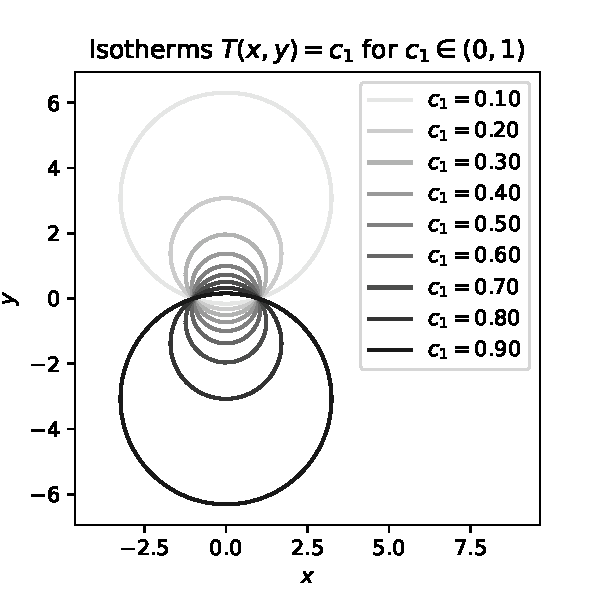
\includegraphics[width=0.45\linewidth]{Python/Steady_Temperatuers_In_Half_Plane}
		\caption*{}
		\label{fig:steadytemperatuersinhalfplane}
	\end{figure}
	
	\subsubsection{Related Problem}
	
	Consider a slab in 3D space that is bounded by planes \(x = \pm \pi/2\) and \(y = 0\), where \(T(x, 0) = 1\) for \(x \in (-\pi/2, \pi/2)\) and \(T(\pi/2, y) = T(-\pi/2, y) = 0\).
	
	Boundary value problem for \(T(x,y)\) bounded:
	\begin{align*}
		T_{xx}(x,y) + T_{yy}(x,y) &= 0
			& x &\in \left(-\frac{\pi}{2}, \frac{\pi}{2}\right), \ y>0 \\
		T\left(-\frac{\pi}{2}, y\right) = T\left(\frac{\pi}{2}, y\right) &= 0
			& y&>0 \\
		T(x,0) &= 1
			& x &\in \left(-\frac{\pi}{2}, \frac{\pi}{2}\right)
	\end{align*}

	We want a transformation that preserves these conditions, so consider the transformation:
	\begin{align*}
		w = g(z) = \sin(z) = \sin(x)\cosh(y) + i \cos(x) \sinh(y)
	\end{align*}
	This transforms the problem into the one we had previously, \(T(x,0) = 1\) along the line segment \(x = \pm 1\) and \(T(x,0) = 0\) for other values of \(x\). (See \cref{Mapping by sine Section - Complex}.)
	 
	\begin{figure}[H]
		\centering
		\begin{tikzpicture}[baseline=(current bounding box.center)]
			\begin{axis}[
				unit vector ratio=1 1 1,
				xlabel={$x$},
				ylabel={$y$},
				xmin=-1.75, xmax=1.75,
				ymin=-0.5, ymax=2.5,
				axis lines = middle,
				ticks=none,
				grid=none,
				]
				
				\draw[line width=1, 
				decoration={markings, mark=at position 1 with {\arrow{>}} },
				postaction={decorate}]
				(axis cs: -1, 0)--(axis cs: -1, 2)
				node[pos=0.25, left] {\(T=0\)}
				node[pos=0, below] {\(-\frac{\pi}{2}\)}
				node[pos=0.5, left] {\(A\)};
				
				\draw[line width=1, 
				decoration={markings, mark=at position 1 with {\arrow{>}} },
				postaction={decorate}]
				(axis cs: 1, 0)--(axis cs: 1, 2)
				node[pos=0.25, right] {\(T=0\)}
				node[pos=0, below] {\(\frac{\pi}{2}\)}
				node[pos=0.5, right] {\(D\)};
				
				\draw[line width=1, dashed, color=White]
				(axis cs: 1, 1)--(axis cs: 1, 1.9);
				
				\draw[line width=1, dashed, color=White]
				(axis cs: -1, 1)--(axis cs: -1, 1.9);
				
				\draw[line width=1, dashed, color=Grey]
				(axis cs: -1, 1)--(axis cs: 1, 1);
				
				\draw[line width=1]
				(axis cs: -1, 0)--(axis cs: 1, 0)
				node[pos=0, above left] {\(B\)}
				node[pos=0.5, below] {\(T=1\)}
				node[pos=1, above right] {\(C\)};
				
				\addplot[
				only marks,
				nodes near coords,
				point meta = explicit symbolic, 
				mark=o,
				]
				coordinates {
					(1, 0) 
					(-1, 0) 
				};
			\end{axis}
		\end{tikzpicture}
		{\Large \(\xrightarrow{\mathmakebox[2cm]{w = g(z)}}\)}
		\begin{tikzpicture}[baseline=(current bounding box.center)]
			\begin{axis}[
				unit vector ratio=1 1 1,
				xlabel={$u$},
				ylabel={$v$},
				xmin=-2.5, xmax=2.5,
				ymin=-0.5, ymax=1.5,
				axis lines = middle,
				ticks = none,
				grid=none,
				]
			
				\addplot[
					only marks,
					nodes near coords,
					point meta = explicit symbolic, 
					mark=o,
					]
					coordinates {
						(2, 0) 
						(1, 0) 
						(0, 0) 
						(-1, 0) 
						(-2, 0) 
					};
				
				\draw[line width=1]
				(axis cs: -2.5, 0) -- (axis cs: 2.5, 0);
				
				\draw[line width=1]
				(axis cs: -2, 0) -- (axis cs: 2, 0)
				node[pos=0, below] {\(D'\)}
				node[pos=0.25, below] {\(C'=-1\)}
				node[pos=0.75, below] {\(B'=1\)}
				node[pos=1, below] {\(A'\)}
				node[pos=0.5, above] {\(T = 1\)}
				node[pos=0.125, above] {\(T = 0\)}
				node[pos=0.875, above] {\(T = 0\)};
				
				\draw[line width=1, dashed, color=Grey]
				(axis cs: -2, 0)--(axis cs: -2, 1)--(axis cs: 2, 1)--(axis cs: 2, 0);
				
				\draw[line width=1, dashed, color=White]
				(axis cs: -2.4, 0) -- (axis cs: -2, 0);
				
				\draw[line width=1, dashed, color=White]
				(axis cs: 2, 0) -- (axis cs: 2.4, 0);
			\end{axis}
		\end{tikzpicture}
	\end{figure}
	
	Using the solution of the boundary value problem we obtained previously:
	\begin{align*}
		T(u,v) &= \frac{1}{\pi} \arctan(\frac{2v}{u^2 + v^2 - 1})
			& \arctan(t) \in [0, \pi]
	\end{align*}
	Applying the transformation:
	\begin{align*}
		T(x,y) 
		&= \frac{1}{\pi} \arctan(\frac{2\cos(x)\sinh(y)}{\sin[2](x)\cosh[2](y) + \cos[2](x)\sinh[2](y) - 1})
	\end{align*}
	Since
	\begin{align*}
		&\frac{2\cos(x)\sinh(y)}{\sin[2](x)\cosh[2](y) + \cos[2](x)\sinh[2](y) - 1} \\
		&= \frac{2 \cos(x) \sinh(y)}{\sinh[2](y) - \cosh[2](x)} 
		 = \frac{2[\cos(x)/\sinh(y)]}{1 - [\cos(x) / \sinh(y)]^2}
		 = \tan(\frac{2\cos(x)}{\sinh(y)})
	\end{align*}
	Hence 
	\begin{align*}
		T &= \frac{2}{\pi} \arctan(\frac{\cos(x)}{\sinh(y)})
			& \arctan(t) \in \left[0, \frac{\pi}{2} \right]
	\end{align*}
	\(\sin(z)\) is entire and \(T(u,v)\) is harmonic in half plane \(v>0\), so \(T(x,y)\) is harmonic in the line \(x \in (-\pi/2, \pi/2)\), \(y>0\). \(T(u,v)\) satisfies boundary condition \(T=1\) for \(\abs{u} < 1\) and \(v=0\), and \(T=0\) for \(\abs{u}>1\) and \(v=0\); hence the boundary conditions for \(T(x,y)\) are satisfied. Moreover, \(\abs{T(x,y)}\leq 1\) in the strip.
	
	Isotherms \(T(x,y) = c_1\), \(c_1 \in (0,1)\), within the slab:
	\begin{align*}
		\cos(x) = \tan(\frac{\pi c_1}{2}) \sinh(y)
	\end{align*}
	The flux of heat into the slab from the surface in \(y=0\) (see \cref{Fourier's Law Definition - Complex}):
	\begin{align*}
		-KT_y(x,0) &= \frac{2K}{\pi \cos(x)}
			& x \in \left(-\frac{\pi}{2}, \frac{\pi}{2}\right)
	\end{align*}
	Outward flux of heat through the plane \(x = \pi/2\):
	\begin{align*}
		-KT_x \left(\frac{\pi}{2}, y\right) &= \frac{2K}{\pi \sinh(y)}
			& y > 0
	\end{align*}
	
	\begin{observation}
		This problem is solved by two transformations, first by \(g(w) = \sin(w) = U + iV\), then \(f(z) = \log[(z-1)/(z+1)] = u + iv\) on the function \(T(U, V)\). 
		
		In order to do so, we transformed the problem into a space where we can solve the problem easily, then transformed it back.
		
			\begin{figure}[H]
			\centering
			\begin{tikzpicture}[baseline=(current bounding box.center)]
				\begin{axis}[
					width=1.5\linewidth,
					unit vector ratio=1 1 1,
					xlabel=none,
					ylabel=none,
					xmin=-2, xmax=2,
					ymin=-1, ymax=1,
					axis lines = none,
					ticks=none,
					grid=none,
					]
					
					\draw[]
					(axis cs: -1, 0) -- (axis cs: -1, 0)
					node[pos=0] {\(z\)-plane};
					
					\draw[]
					(axis cs: 0, 0) -- (axis cs: 0, 0)
					node[pos=0] {\(w\)-plane};
					
					\draw[]
					(axis cs: 1, 0) -- (axis cs: 1, 0)
					node[pos=0] {\(W\)-plane};
					
					\draw[line width=1, 
					decoration={markings, mark=at position 1 with {\arrow{>}} },
					postaction={decorate}]
					(axis cs: -0.9, 0.1) arc (120:60:80)
					node[pos=0.5, above] {\(w=f(z)\)};
					
					\draw[line width=1, 
					decoration={markings, mark=at position 1 with {\arrow{>}} },
					postaction={decorate}]
					(axis cs: 0.1, 0.1) arc (120:60:80)
					node[pos=0.5, above] {\(W = g(w)\)};
					
					\draw[line width=1, 
					decoration={markings, mark=at position 1 with {\arrow{>}} },
					postaction={decorate}]
					(axis cs: 0.9, -0.1) arc (-60:-120:80)
					node[pos=0.5, below] {Sub: \(U(u,v)\) and \(V(u,v)\)};
					
					\draw[line width=1, 
					decoration={markings, mark=at position 1 with {\arrow{>}} },
					postaction={decorate}]
					(axis cs: -0.1, -0.1) arc (-60:-120:80)
					node[pos=0.5, below] {Sub: \(u(x,y)\) and \(v(x,y)\)};
				\end{axis}
			\end{tikzpicture}
		\end{figure}
	
		The strategy of employed here seems to be mapping the boundary with the conditions onto a line (the \(u\) axis here), then map that line into a plane that with different boundary conditions on separate parallel lines. This ensures a simple solution in that plane, which we can solve, then transform back to the original plane. 
	\end{observation}
	
	\subsection{Temperatures in a Quadrant} \label{Temperatures in a Quadrant Subsection - Complex}
	\index{Temperature! Time Independent! Quadrant}
	
	Consider a quadrant where one edge is kept at a fixed temperature, the end of the other edge is insulated while the rest is kept at another temperature.
	
	Boundary conditions:
	\begin{align*}
		T_{xx}(x,y) + T_{yy}(x,y) &= 0 &
			x&>0, \ y>0 \\
		T_y(x,0) &= 0 & x &\in (0,1) \\
		T(x,0) &= 1 & x&>1 \\
		T(0,y) &= 0 & y&>0
	\end{align*}
	\(T(x,y)\) is bounded in the quadrant. Boundary conditions are of types \(h = h_0\) and \(\dv*{h}{n} = 0\).
	
	Transformation:
	\begin{align*}
		w = f(z) = \sin[-1](z)
	\end{align*}
	
	The existence of this inverse is ensured by the bijective nature of the transform. The transformation is conformal except at \(w = \pi/2\), hence it is not conformal at \(z = 1\).
	
	Boundary conditions suggest the temperature function:
	\begin{align*}
		T = \frac{2}{\pi} u
	\end{align*}
	We know that 
	\begin{align*}
		x &= \sin(u)\cosh(v)	&
		y &= \cos(u)\sinh(v)
	\end{align*}
	Hence, \(x\) and \(y\) nonzero in \((0, \pi/2)\). Consequently
	\begin{align*}
		\cosh[2](v) - \sinh[2](v) = \frac{x^2}{\sin[2](u)} - \frac{y^2}{\cos[2](u)} = 1
	\end{align*}
	For fixed \(u\), this is hyperbola with foci
	\begin{align*}
		z = \pm \sqrt{\sin[2](u) + \cos[2](u)} = \pm 1
	\end{align*}

	The length of the transverse axis (length of line joining two vertices \((\pm \sin(u), 0)\)) is \(2\sin(u)\). Distances between a foci and point on hyperbola:
	\begin{align*}
		\sqrt{(x+1)^2 + y^2} - \sqrt{(x-1)^2 + y^2} = 2\sin(u)
	\end{align*}
	Then
	\begin{align*}
		T &= \frac{2}{\pi} \sin[-1](\frac{\sqrt{(x+1)^2 + y^2} - \sqrt{(x-1)^2 + y^2}}{2})
			& u\in \left[0, \frac{\pi}{2}\right]
	\end{align*}
	Temperature along the lower edge of plate:
	\begin{align*}
		T(x,0) = \frac{2}{\pi} \sin[-1](x)
	\end{align*}
	Isotherms \(T(x,y) = c_1\), \(c_1 \in (0,1)\), are parts of the confocal hyperbola where \(u = \pi c_1 /2\) in the first quadrant. Lines of flow are then the confocal ellipses for constant \(v\), since \(2v/\pi\) is the harmonic conjugate of \(T(u,v) = 2u/\pi\).
	
	\begin{figure}[H]
		\centering
		\begin{tikzpicture}[baseline=(current bounding box.center)]
			\begin{axis}[
				unit vector ratio=1 1 1,
				xlabel={$x$},
				ylabel={$y$},
				xmin=-0.75, xmax=2.5,
				ymin=-0.2, ymax=2.5,
				axis lines = middle,
				ticks=none,
				grid=none,
				]
				
				\draw[line width=1,]
				(axis cs: 0, 0)--(axis cs: 0, 2)
				node[pos=0, above left] {\(C\)}
				node[pos=1, left] {\(D\)}
				node[pos=0.5, left] {\(T=0\)};
				
				\draw[line width=1, color=Grey]
				(axis cs: 0, 0)--(axis cs: 0.5, 0);
				
				\draw[line width=1,]
				(axis cs: 0.5, 0)--(axis cs: 2, 0)
				node[pos=0, above] {\(B\)}
				node[pos=1, above] {\(A\)}
				node[pos=0, below] {\(1\)}
				node[pos=0.5, above] {\(T=1\)};
				
				\draw[line width=1,
				decoration={markings, mark=at position 1 with {\arrow{>}} },
				postaction={decorate}]
				(axis cs: 2, 0)--(axis cs: 2.3, 0);
				
				\draw[line width=1, dashed, color=White]
				(axis cs: 2, 0)--(axis cs: 2.4, 0);
				
				\draw[line width=1,
				decoration={markings, mark=at position 1 with {\arrow{>}} },
				postaction={decorate}]
				(axis cs: 0, 2)--(axis cs: 0, 2.3);
				
				\draw[line width=1, dashed, color=White]
				(axis cs: 0, 2)--(axis cs: 0, 2.4);
				
				\addplot[
				only marks,
				nodes near coords,
				point meta = explicit symbolic, 
				mark=o,
				]
				coordinates {
					(0, 0) 
					(0.5, 0) 
				};
			\end{axis}
		\end{tikzpicture}
		{\Large \(\xrightarrow{\mathmakebox[2cm]{w = f(z)}}\)}
		\begin{tikzpicture}[baseline=(current bounding box.center)]
			\begin{axis}[
				unit vector ratio=1 1 1,
				xlabel={$u$},
				ylabel={$v$},
				xmin=-0.5, xmax=1.5,
				ymin=-0.2, ymax=1.6,
				axis lines = middle,
				ticks = none,
				grid=none,
				]
				
				\addplot[
				only marks,
				nodes near coords,
				point meta = explicit symbolic, 
				mark=o,
				]
				coordinates {
					(0, 0) 
					(1, 0)
				};
				
				\draw[line width=1]
				(axis cs: 0, 0) -- (axis cs: 0, 1)
				node[pos=0, above left] {\(C'\)}
				node[pos=0.5, left] {\(T=0\)}
				node[pos=1, left] {\(D'\)};
				
				\draw[line width=1]
				(axis cs: 1, 0) -- (axis cs: 1, 1)
				node[pos=0, above right] {\(B'\)}
				node[pos=1, right] {\(A'\)}
				node[pos=0, below] {\(\pi/2\)}
				node[pos=0.5, right] {\(T=1\)};
				
				\draw[line width=1, color=Grey]
				(axis cs: 0, 0) -- (axis cs: 1, 0);
				
				\draw[line width=1,
				decoration={markings, mark=at position 1 with {\arrow{>}} },
				postaction={decorate}]
				(axis cs: 0, 1)--(axis cs: 0, 1.5);
				
				\draw[line width=1, dashed, color=White]
				(axis cs: 0, 1) -- (axis cs: 0, 1.4);
				
				\draw[line width=1,
				decoration={markings, mark=at position 1 with {\arrow{>}} },
				postaction={decorate}]
				(axis cs: 1, 1)--(axis cs: 1, 1.5);
				
				\draw[line width=1, dashed, color=White]
				(axis cs: 1, 1) -- (axis cs: 1, 1.4);
				
				\addplot[
				only marks,
				nodes near coords,
				point meta = explicit symbolic, 
				mark=o,
				]
				coordinates {
					(0, 0) 
					(1, 0) 
				};
			\end{axis}
		\end{tikzpicture}
	\end{figure}
	
	\begin{figure}[H]
		\centering
		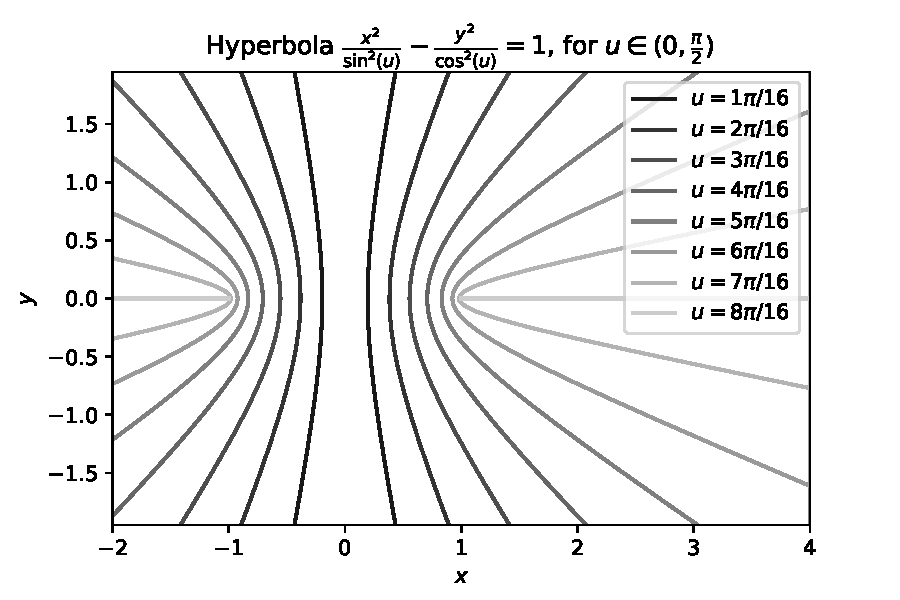
\includegraphics[width=0.7\linewidth]{Python/Temperaturues_in_Quadrant_Hyperbola}
		\caption*{}
		\label{fig:temperaturuesinquadranthyperbola}
	\end{figure}
	
	\subsection{Electrostatic Potential} \label{Electrostatic Potential Subsection - Complex}
	\index{Electrostatic! Potential}
	
	In any charge free region, the potential in the region due to charges exterior to the region satisfies Laplace's equation for 3D space. Then the potential for 2D space:
	\begin{align*}
		V_{xx}(x,y) + V_{yy}(x,y) = 0
	\end{align*}
	Lines \(V(x,y) = c_1\) are equipotential lines.
	If \(U\) is a harmonic conjugate of \(V\), then lines \(U(x,y) = c_2\) are flux lines. At any point \((x,y)\) where \(\dv*{z} [V(x,y) + iU(x,y)] \neq 0\), then the two curves are orthogonal. Boundary value problems from \cref{Time Independent Temperatures Subsection - Complex} can then be applied here.
	
	\begin{example}
		Consider a cylinder of unit radius in the \(z\) plane. The top half (\(y>0\)) has \(V(x,y) = 0\), while the bottom half \(y<0\) has \(V(x,y) = 1\)
		
		We are dealing with a circle, so we can use a linear fractional transformation (\cref{Linear Fractional Transformations Section - Complex}). Using the inverse of \(f^{-1}(w)\) we find:
		\begin{align*}
			f^{-1}(w) = z = \frac{i - w}{i + w} 
			\implies f(z) = w = i \frac{1 - z}{1 + z}
		\end{align*}
		Now
		\begin{align*}
			\frac{1}{\pi} \operatorname{Log}(w)
			&= \frac{1}{\pi} \ln(\rho) + i \frac{1}{\pi} \phi
				& \rho > 0, \ \phi \in [0, \pi]
		\end{align*}
		which the imaginary part is bounded and satisfies \(V(u,v) = 0\) for \(\phi = 0\) and \(V(u,v) = 1\) for \(\phi = \pi\). The harmonic function for the half plane:
		\begin{align*}
			V(u, v) &= \frac{1}{\pi} \tan[-1](\frac{v}{u})
				& \tan[-1](\frac{u}{v}) \in [0, \pi]
		\end{align*}
		Applying transformation:
		\begin{align*}
			V(x,y) &= \frac{1}{\pi} \tan[-1](\frac{1-x^2-y^2}{2y})
				& \tan[-1](\frac{1-x^2-y^2}{2y}) \in [0, \pi]
		\end{align*}
		This is the potential function within the cylinder. To verify the solution, note:
		\begin{align*}
			\lim_{t\rightarrow0, \ t>0} \tan[-1](t) &= 0 	&
			\lim_{t\rightarrow0, \ t<0} \tan[-1](t) &= \pi 
		\end{align*}
		The equipotential curves \(V(x,y) = c_1\), \(c_1 \in (0, 1)\), are circles that pass through \((\pm 1, 0)\):
		\begin{align*}
			x^2 + [y + \tan(\pi c_1)]^2 = \sec[2](\pi c_1)
		\end{align*}
		It's clear that for the segment on \(x\) axis \(V(x, 0) = 1/2\), \(x \in (-1, 1)\). 
		
		\(U\) is the harmonic conjugate of \(V\), hence
		\begin{align*}
			U 
			= -\frac{1}{\pi}\ln(\rho) 
			= \Im{-\frac{i}{\pi}\operatorname{Log}(w)} 
			= - \frac{1}{\pi} \ln\abs{\frac{1-z}{1+z}}
		\end{align*}
		The flux lines \(U(x,y) = c_2\) are then circles with centers on the \(x\) axis.
		
		\begin{figure}[H]
			\centering
			\begin{tikzpicture}[baseline=(current bounding box.center)]
				\begin{axis}[
					unit vector ratio=1 1 1,
					xlabel={$x$},
					ylabel={$y$},
					xmin=-1.5, xmax=1.5,
					ymin=-1.5, ymax=1.5,
					axis lines = middle,
					ticks=none,
					grid=none,
					]
					
					\draw[line width=1,]
					(axis cs: -1, 0) arc (-180:180:100)
					node[pos=0, 	below left]	{\(A\)}
					node[pos=0.25, 	below] 		{\(V=1\)}
					node[pos=0.25, 	above] 		{\(B\)}
					node[pos=0.5, 	right] 		{\(C\)}
					node[pos=0.75,	below] 		{\(D\)}
					node[pos=0.75, 	above] 		{\(V=0\)}
					node[pos=1, 	above left] {\(E\)};
					
					\addplot[
					only marks,
					nodes near coords,
					point meta = explicit symbolic, 
					mark=o,
					]
					coordinates {
						(1, 0) 
						(-1, 0) 
					};
				\end{axis}
			\end{tikzpicture}
			{\Large \(\xrightarrow{\mathmakebox[2cm]{w = f(z)}}\)}
			\begin{tikzpicture}[baseline=(current bounding box.center)]
				\begin{axis}[
					unit vector ratio=1 1 1,
					xlabel={$u$},
					ylabel={$v$},
					xmin=-2, xmax=2,
					ymin=-0.4, ymax=2,
					axis lines = middle,
					ticks = none,
					grid=none,
					]
					
					\addplot[
					only marks,
					nodes near coords,
					point meta = explicit symbolic, 
					mark=o,
					]
					coordinates {
						(0, 0) 
					};
				
					\addplot[
					only marks,
					nodes near coords,
					point meta = explicit symbolic, 
					mark=*,
					]
					coordinates {
						(-0.5, 0) 
						(0.5, 0)
						(1, 1)
					};
					
					\draw[]
					(axis cs: 0, 0) -- (axis cs: 1, 1)
					node[pos=0.5, 	above left] 	{\(\rho\)}
					node[pos=1, 	above right] 	{\(w\)};
					
					\draw[line width=1]
					(axis cs: -2, 0) -- (axis cs: 2, 0);
					
					\draw[line width=1, dashed, color=Grey]
					(axis cs: 1.5, 0) -- (axis cs: 1.5, 1.75) -- (axis cs: -1.5, 1.75) -- (axis cs: -1.5, 0);
					
					\draw[line width=1]
					(axis cs: -1.5, 0) -- (axis cs: 1.5, 0)
					node[pos=0, 	above] {\(A'\)}
					node[pos={1/3}, above] {\(B'\)}
					node[pos=0.5, 	above] {\(C'\)}
					node[pos={2/3}, above] {\(D'\)}
					node[pos=1, 	above] {\(E'\)}
					node[pos={2/3}, below] {\(1\)}
					node[pos={1/6}, below] {\(V=1\)}
					node[pos={5/6}, below] {\(V=0\)};
					
					\draw[
					decoration={markings, mark=at position 1 with {\arrow{>}} },
					postaction={decorate}]
					(axis cs: 1, 0) arc (0:45:100)
					node[pos=0.5, right] {\(\phi\)};
					
					\draw[line width=1, dashed, color=White]
					(axis cs: -1.5, 0) -- (axis cs: -1.9, 0);
					
					\draw[line width=1, dashed, color=White]
					(axis cs: 1.5, 0) -- (axis cs: 1.9, 0);
				\end{axis}
			\end{tikzpicture}
		\end{figure}
	\end{example}
	
	\begin{example}
		Consider the following boundary conditions for \(V(r, \theta)\):
		\begin{align*}
			V(r_0, \theta) &= 0 
				& r_0 > 1, \ \theta \in [0,\pi] \\
			V(1, \theta) &= 0 
				& r_0 > 1, \ \theta \in [0,\pi] \\
			V(x, 0) &= 0 
				& x \in [1, r_0] \\
			V(x, \pi) &= 1 
				& x \in [1, r_0] \\
		\end{align*}
		We can solve for \(V(r,\theta)\) using separation of variables:
		\begin{align*}
			V 
			&= \frac{4}{\pi} \sum_{n=1}^{\infty} \frac{\sinh(\alpha_n v)}{\sinh(\alpha_n \pi)} \cdot \frac{\sin(\alpha_n)}{2n-1}	&
			\alpha_n &= \frac{(2n-1)\pi}{\ln(r_0)}	&
				n \in \mathbb{N}
		\end{align*}
		Transformation with branch:
		\begin{align*}
			\log(z) &= \ln(r) + i \theta &
				r>0, \ -\frac{\pi}{2} < \theta < \frac{3\pi}{2}
		\end{align*}
		The transformation is a injective mapping of the regions. Since the \(u\) and \(v\) are harmonic:
		\begin{align*}
			V(r, \theta)
			&= \frac{4}{\pi} \sum_{n=1}^{\infty} 
				\frac{\sinh(\alpha_n \theta)}{\sinh(\alpha_n \pi)} \cdot \frac{\sin(\alpha_n \ln(r))}{2n-1} 	&
			\alpha_n &= \frac{(2n-1)\pi}{\ln(r_0)}	&
			n \in \mathbb{N}
		\end{align*}
	
		\begin{figure}[H]
			\centering
			\begin{tikzpicture}[baseline=(current bounding box.center)]
				\begin{axis}[
					unit vector ratio=1 1 1,
					xlabel={$x$},
					ylabel={$y$},
					xmin=-1.5, xmax=1.5,
					ymin=-0.2, ymax=1.5,
					axis lines = middle,
					ticks=none,
					grid=none,
					]
					
					\draw[line width=1,]
					(axis cs: 1, 0) arc (0:180:100)
					node[pos=0.5, above] {\(V = 0\)};
					
					\draw[line width=1,]
					(axis cs: 0.25, 0) arc (0:180:25)
					node[pos=0.5, above] {\(V = 0\)};
					
					\draw[line width=1,]
					(axis cs: 0.25, 0) -- (axis cs: 1, 0)
					node[pos=0, below] {1}
					node[pos=0.5, above] {\(V = 0\)}
					node[pos=1, below] {\(r_0\)};
					
					\draw[line width=1,]
					(axis cs: -0.25, 0) -- (axis cs: -1, 0)
					node[pos=0.5, above] {\(V = 1\)};
					
					\addplot[
					only marks,
					nodes near coords,
					point meta = explicit symbolic, 
					mark=o,
					]
					coordinates {
						(1, 0) 
						(0.25, 0) 
					};
				
					\addplot[
					only marks,
					nodes near coords,
					point meta = explicit symbolic, 
					mark=o,
					]
					coordinates {
						(-1, 0) 
						(-0.25, 0) 
					};
				\end{axis}
			\end{tikzpicture}
			{\Large \(\xrightarrow{\mathmakebox[2cm]{w = f(z)}}\)}
			\begin{tikzpicture}[baseline=(current bounding box.center)]
				\begin{axis}[
					unit vector ratio=1 1 1,
					xlabel={$u$},
					ylabel={$v$},
					xmin=-0.5, xmax=2.5,
					ymin=-0.25, ymax=1.5,
					axis lines = middle,
					ticks = none,
					grid=none,
					]
					
					\addplot[
					only marks,
					nodes near coords,
					point meta = explicit symbolic, 
					mark=o,
					]
					coordinates {
						(2, 1) 
						(0, 1)
					};
					
					\addplot[
					only marks,
					nodes near coords,
					point meta = explicit symbolic, 
					mark=*,
					]
					coordinates {
						(2, 0) 
					};
					
					\draw[line width=1]
					(axis cs: 0, 0) -- (axis cs: 2, 0)
					node[pos=0.5, above] {\(V = 0\)}
					node[pos=1, below] {\(\ln(r_0)\)};
					
					\draw[line width=1]
					(axis cs: 2, 0) -- (axis cs: 2, 1)
					node[pos=0.5, right] {\(V = 0\)};
					
					\draw[line width=1]
					(axis cs: 2, 1) -- (axis cs: 0, 1)
					node[pos=0.5, above] {\(V = 1\)}
					node[pos=1, left] {\(\pi i\)};
					
					\draw[line width=1]
					(axis cs: 0, 1) -- (axis cs: 0, 0)
					node[pos=0.5, left] {\(V = 0\)};
				\end{axis}
			\end{tikzpicture}
		\end{figure}
	\end{example}
	
	\subsection{2D Fluid Flow} \label{2D Fluid Flow Subsection - Complex}
	\index{Fluid Flow! 2D}
	
	Consider a motion of a sheet of fluid in the \(z\) plane. The velocity of the fluid:
	\begin{align*}
		V(x,y) = p(x,y) + iq(x,y)
	\end{align*}
	\(p(x,y)\) and \(q(x,y)\) are \(\hat{x}\) and \(\hat{y}\) components of the velocity vector. In a region without sinks or sources, their first-order partial derivatives are continuous. 
	
	\begin{definition}[Circulation]
		\label{Circulation Definition - Complex}
		\index{Circulation}
		The line integral with respoct to arc length \(\sigma\) of the tangential component of the velocity vector \(V_T(x,y)\) along contour \(C\).
		\begin{align*}
			\int_{C} V_T(x,y) d\sigma = \int_{C} p(x,y) dx + q(x,y) dy
		\end{align*}
	\end{definition}
	If \(C\) is a positively oriented simple closed contour in a simply connected domain with no sources or sinks, we can use Green's Theorem (\cref{Green's Theorem - ODE}):
	\begin{align*}
		\int_C V_T(x,y) d\sigma = \iint_{R} [q_x(x,y) + p_y(x,y)] dA
	\end{align*}
	
	For a circular region centered about \((x_0, y_0)\), the mean speed along \(C\) is found by dividing the circulation by \(2\pi r\). Dividing the mean speed by \(r\) gets the mean angular speed:
	\begin{align*}
		\frac{l}{\pi r^2} \iint_{R} \frac{1}{2} [q_x(x,y) + p_y(x,y)] dA
	\end{align*}
	
	\begin{definition}[Rotation (Fluid)]
		\label{Rotation of Fluid Definition - Complex}
		\index{Rotation! Fluid}
		The limiting angular speed as the radius \(r \rightarrow 0\).
		\begin{align*}
			\omega (x,y) =  \frac{1}{2} [q_x(x,y) + p_y(x,y)]
		\end{align*}
	\end{definition}
	The mean value of the rotation is the mean angular velocity of the fluid. 

	\begin{definition}[Irrotational (Fluid)]
		\label{Irrotational Fluid Definition - Complex}
		\label{Irrotational! Fluid}
		When the rotation is zero.
		\[w(x,y) = 0\]
	\end{definition}
	
	For a incompressible and non-viscous fluid of uniform density \(\rho\), the fluid pressure \(P(x,y)\) with velocity \(V(x,y)\) satisfies a special case of Bernoulli's Equation \index{Bernoulli's Equation}: 
	\begin{align*}
		\frac{P(x,y)}{\rho} + \frac{1}{2} \abs{V(x,y)}^2 = c
	\end{align*}
	
	For an irrotational fluid:
	\begin{align*}
		\omega (x,y) =  \frac{1}{2} [q_x(x,y) + p_y(x,y)] = 0
		\implies \int_{C} p(s,t) ds + q(s,t) dt = 0
	\end{align*}
	That is, the contour \(C\) is independent of path. Hence,
	\begin{align*}
		\phi(x,y) = \int_{(x_0, y_0)}^{(x,y)} p(s,t) ds + q(s,t) dt
	\end{align*}
	is well defined on domain \(D\). Taking the partial derivatives
	\begin{align*}
		\phi_x(x,y) &= p(x,y) &
		\phi_y(x,y) &= q(x,y)
	\end{align*}
	shows \(\phi(x,y)\) is the velocity potential of velocity vector \(V = p + iq\).
	Likewise, in a region of free of sources and sinks, \(\phi(x,y)\) satisfies Laplace's equation and is harmonic:
	\begin{align*}
		\phi_{xx}(x,y) + \phi_{yy}(x,y) = 0
	\end{align*}
	
	\subsection{Stream Function} \label{Stream Function Subsection - Complex}
	\index{Stream Function}
	
	The velocity vector in a irrotational simply connected domain:
	\begin{align*}
		V = p(x,y) + iq(x,y) = \phi_x(x,y) + i \phi_y(x,y) = \grad{\phi(x,y)}
	\end{align*}

	\begin{definition}[Stream Function]
		\label{Stream Function Definition - Complex}
		\index{Stream Function}
		The harmonic conjugate of the velocity potential \(\phi(x,y)\):
		\begin{align*}
			\psi(x,y)
		\end{align*}
	\end{definition}
	
	\begin{definition}[Streamlines]
		Curves of equal value in \(\psi(x,y)\):
		\begin{align*}
			\psi(x,y) = c_2
		\end{align*}
	\end{definition}
	Velocity vectors are tangent to the stream lines.
	
	\begin{definition}[Complex Potential (Flow)]
		\label{Complex Potential (Flow) Definition - Complex}
		\index{Complex Potential! Flow}
		\begin{align*}
			F(z) = \phi(x,y) + i \psi(x,y)
		\end{align*}
	\end{definition}
	
	Taking the derivative and using Cauchy-Riemann equations (\cref{Cauchy-Riemann Equations (Cartesian) Theorem - Complex}).
	\begin{align*}
		F'(z) = \phi_x(x,y) + i\psi_x(x,y) = \phi_x(x,y) - i \phi_y(x,y)
	\end{align*}
	Hence the velocity
	\begin{align*}
		V = \overline{F'(z)}
	\end{align*}
	
	According to the proof of \cref{Harmonic Function on Simply Connected Domain always have harmonic conjugate v Theorem - Complex}, we can write
	\begin{align*}
		\psi(x,y) 
		&= \int_{(x_0, y_0)}^{(x,y)} - \phi_t(s,t) ds + \phi_s(s,t) dt \\
		&= \int_C - q(s,t) ds + p(s,t) dt
		&= \int_{C} V_N (s,t) d\sigma
	\end{align*}
	which is independent of path, and \(C\) is any contour in \(D\). \(V_N\) is the normal component of the velocity vector, and \(\sigma\) is te arc length along \(C\). Then \(\psi(x,y)\) is the rate of flow across a surface of unit height perpendicular to the \(z\) plane on the curve \(C\).
	
	\begin{example}
		Consider 
		\begin{align*}
			F(z) &= Az & A \in \mathbb{R}_{>0}
		\end{align*}
		Then
		\begin{align*}
			\phi(x,y) &= Ax &
			\psi(x,y) &= Ay
		\end{align*}
		Streamlines \(\psi(x,y) = c_2 \implies y = c_2 /A\), and velocity \(V = \overline{F'(z)} = A\). The point \((x_0, y_0)\) where \(\psi(x_0, y_0) = 0\) is then any point on the \(x\) axis. 
		
		Here we can see a harmonic functions that is not uniquely determined up to an additive constant due to the boundary values. \(\psi(x,y) = Ay\) is harmonic in half plane \(y>0\) and is zero at the boundaries. \(\psi_1(x,y) = Be^x \sin(y)\) also satisfies the boundary conditions, but \(\psi_1(x,y) = 0\) consists of \(y = 0\) and \(y = n \pi\), (\(n \in \mathbb{N}\)). \(F_1(z) = Be^z\) is the complox potential of the flow between \(y \in [0, \pi]\), both boundaries making up \(\psi(x,y) = 0\). If \(B>0\), the fluid flows to the right along \(y = 0\) and left along \(y = \pi\).
	\end{example}

	\subsection{Flow Around Corner and Cylinder} \label{Flow Around Corner and Cylinder Subsection - Complex}
	
	If transformation \(f(z): D_z \rightarrow D_w\), is an analytic function:
	\begin{align*}
		w = f(z) = u(x,y) + iv(x,y)
	\end{align*}
	Then the functions are harmonic in \(D_z\):
	\begin{align*}
		\phi[u(x,y), v(x,y)] &&& \psi[u(x,y), v(x,y)]
	\end{align*}
	These are the velocity potential and stream function in the \(z\) plane. Streamline or boundary \(\psi(u,v) = c_2\) in \(D_w\) implies \(\psi[u(x,y), v(x,y)] = c_2\) in \(D_z\).
	
	It is often efficient to write the complex potential function in \(D_w\), then use it to obtain the corresponding function in the \(z\) plane. That is use
	\begin{align*}
		F(w) = \phi(u,v) + i\psi(u,v)
	\end{align*}
	to obtain
	\begin{align*}
		F[f(z)] = \phi[u(x,y), v(x,y)] + i \psi[u(x,y), v(x,y)]
	\end{align*}
	
	\begin{example}[Flow around a corner]
		\label{Flow around a corner Example - Complex}
		\label{Flow! Around a corner}
		Consider a flow in the first quadrant, where the flow is comes parallel to the \(y\) axis but has to turn the corner to the \(x\) axis.
		We use the transformation to map the boundary of the first quadrant to the entire \(u\) axis:
		\begin{align*}
			w = z^2 = x^2 - y^2 + i2xy
		\end{align*}
		The complex potential function for uniform flow to the right in the \(w\) plane:
		\begin{align*}
			F &= Aw &
			A \in \mathbb{R}
		\end{align*}
		Therefore
		\begin{align*}
			F = Az^2 = A(x^2 - y^2) + i2Axy
		\end{align*}
		Stream function \(\psi\) is then harmonic the first quadrant and vanishes on the boundary:
		\begin{align*}
			\psi = 2Axy
		\end{align*}
		The streamlines are the hyperbolas \(2Axy = c_2\).
		Velocity of the fluid:
		\begin{align*}
			V = \overline{2Az} = 2A(x - iy)
		\end{align*}
		With speed
		\begin{align*}
			\abs{V} &= 2A \sqrt{x^2 + y^2} \propto r
				& r = \sqrt{x^2 + y^2}
		\end{align*}
	\end{example}

	\begin{example}[Flow around a cylinder]
		\label{Flow around a cylinder Example - Complex}
		\label{Flow! Around a cylinder}
		Consider a cylinder of unit radius perpendicular to the \(z\) plane and placed at the origin of the \(z\) plane. The flow is steady and in the positive \(x\) direction. Symmetry shows points on the \(x\) axis exterior to the circle may be treated as boundary points, therefore, consider the upper half plane. 
		
		We map the upper semicircle and the \(x\) axis exterior to the circle to the entire \(u\) axis, and the region to the upper half plane \(v \geq 0\) by transformation:
		\begin{align*}
			w = z + \frac{1}{z}
		\end{align*}
		Complex potential for uniform flow:
		\begin{align*}
			F = Aw \implies F = A\left( z + \frac{1}{z} \right)
		\end{align*}
		Velocity:
		\begin{align*}
			V = A \left(1 - \frac{1}{\bar{z}^2}\right)
		\end{align*}
		Thus flow is approaches uniformity for large \(\abs{z}\). Since \(V(\bar{z}) = \overline{V(z)}\), we can use the reflection principle (\cref{Reflection Principle Theorem - Complex}) to verify that the expression also represents flow in the lower half plane.
		
		The stream function in polar:
		\begin{align*}
			\psi = A \left(r - \frac{1}{r}\right) \sin(\theta)
		\end{align*}
		Stream lines
		\begin{align*}
			A \left( r - \frac{1}{r}\right) \sin(\theta) = c_2
		\end{align*}
		are symmetric to the \(y\) axis with asymptotes parallel to the \(x\) axis. Note:
		\(c_2 = 0\), the stream line consists of circle \(r = 1\) and the \(x\) axis exterior to the circle.
	\end{example}

	\begin{observation}
		Strategy seems to be find a function that expresses the complex potential in \(D_w\), find a transformation \(f(z): D_z \mapsto D_w\) that maps the problem from \(D_z\) to \(D_w\) where it is easier to solve while satisfying the boundary conditions, then map it back to \(D_z\) using the transformation. 
	\end{observation}
	
	{\color{Red} \textbf{Note to self:} Need to do questions in chapter 10 of Brown and Churchill - Complex Variables and Applications (9th ed). (Skipped due to time constraints.)}
	
	\chapter{Schwarz-Christoffel Transformtion} \label{Schwarz-Christoffel Transformation Chapter - Complex}
	
	Schwarz-Christoffel transformation is a mapping of the \(x\) axis and the upper half of the \(z\) plane onto a polygon and its interior in the \(w\) plane
	
	\section{Mapping the Real Axis onto a Polygon} \label{Mapping the Real Axis onto a Polygon Section - Complex}
	
	\index{Mapping! Real Axis onto Polygon}
	
	Let \(C\) be a smooth arc with image \(\Gamma\) under the transformation \(w = f(z)\). The unit vector tangent to \(C\) at \(z_0\) is denoted by \(t \in \mathbb{C}\), and the corresponding unit vector tangent to \(\Gamma\) at \(w_0\) is \(\tau\). Assuming \(f\) is analytic at \(z_0\) and \(f'(z_0) \neq 0 \):
	\begin{align*}
		\arg(\tau) = \arg[f'(z_0)] + \arg(t)
	\end{align*}
	If \(C\) is a segment of the \(x\) axis moving in a positive sense to the right, then \(t = 1\) and \(\arg(t) = 0\) for all \(z_0\) on \(C\). The equation becomes:
	\begin{align*}
		\arg(\tau) = \arg[f'(x)]
	\end{align*}
	\(\arg[f'(z)] = c \implies \arg(\tau) = c\), thus, \(\Gamma\) is also a segment of a straight line. 
	
	Let \(x_1, x_2, \ldots, x_{n-1}\) and \(\infty\), \(x_1<x_2<\cdots<x_{n-1}\) be points on the \(x\) axis with the image under \(f(z)\) be vertices of the polygon:
	\begin{align*}
		w_j &= f(x_j) &
		w_n &= f(\infty) &
		j \in \{1, 2, \ldots , n-1\}
	\end{align*}
	\(\arg[f(z)]\) jumps from one constant value to another at \(z=x_j\) as \(z\) traces the \(x\) axis. Choose \(f(z)\) such that:
	\begin{align*}
		f'(z) &= A(z - x_1)^{-k_1} (z-x_2)^{-k_2} \cdots (z-x_{n-1})^{-k_{n-1}} &
		A \in \mathbb{C}, \ k_j \in \mathbb{R}
	\end{align*}
	Then \(\arg[f'(z)]\) changes in prescribed manner as \(z\) describes the real axis:
	\begin{align*}
		arg[f'(z)] = \arg(A) - k_1 \arg(z - x_1) - k_2 \arg(z-x_2) - \cdots - k_{n-1} \arg(z - x_{n-1})
	\end{align*}
	For \(z = x\) and \(x < x_1\):
	\begin{align*}
		\arg(z-x_1) = \arg(z-x_2) = \cdots = \arg(z-x_{n-1}) = \pi
	\end{align*}
	If \(x_i < x\), then \(\arg(x_i - x) = 0\), and if \(x < x_j\) then \(\arg(x_j - x) = \pi\). \(\arg[f'(z)]\) then jumps by \(k_j \pi\) as \(z\) crosses \(z = x_j\). Likewise, the direction of \(\tau\) changes by \(k_j \pi\) at \(w_j\). The exterior angles are limited to \((-\pi, \pi)\), so \(k_j \in (-1, 1)\).
	
	Assuming the sides of the polygon never cross and the polygon is in a positive orientation, the sum of the angles for a closed polygon is \(2\pi\):
	\begin{align*}
		k_n \pi = 2\pi - (k_1 + k_2 + \cdots + k_{n-1}) \pi
	\end{align*}
	Then \(k_j\) must satisfy
	\begin{align*}
		k_1 + k_2 + \cdots + k_{n-1} + k_n &= 2 &
		k_j &\in (-1, 1) &
		j &\in \{1, 2, 3, \ldots, n\}
	\end{align*}
	Note:
	\begin{align*}
		k_1 + k_2 + \cdots + k_{n-1} = 2 \implies k_n = 0
	\end{align*}
	So, direction of \(\tau\) does not change at \(w_n\), thus \(w_n\) is not a vertex. The polygon has \(n - 1\) sides. 
	
	\section{Schwarz-Christoffel Transformation} \label{Schwarz-Christoffel Transformation Section - Complex} 
	
	\begin{theorem}[Schwarz-Christoffel Transformation]
		\label{Schwarz-Christoffel Transformations Theorem - Complex}
		\index{Schwarz-Christoffel Transformation}
		\begin{align*}
			w 
			&= A \int_{z_0}^{z} (s-x_1)^{-k_1} (s-x_2)^{-k_2} \cdots (s-x_{n-1})^{-k_{n-1}} ds + B &
			B \in \mathbb{C}
		\end{align*}
	\end{theorem}
	\begin{proof}
		A function mapping the \(x\) axis onto a polygon:
		\begin{align*}
			f'(z) &= A(z - x_1)^{-k_1} (z-x_2)^{-k_2} \cdots (z-x_{n-1})^{-k_{n-1}} &
			A \in \mathbb{C}
		\end{align*}
		Let 
		\begin{align*}
			(z-x_j)^{-k_j} 
			&= e^{-k_j \log(z-x_j)} = e^{-k_j(\ln\abs{z-x_j} + i\theta_j)} &
				\theta_j \in \left(-\frac{\pi}{2}, \frac{3\pi}{2}\right) \\
			&= \abs{z - x_j}^{-k_j}	e^{-k_j \theta_j} &
				\theta_j = \arg(z - x_j), \ j \in \{1, 2, \ldots, n-1\}
		\end{align*}
		\(f'(z)\) is then analytic everywhere in half plane \(y\geq 0\) except at \(x_j\).
	\end{proof}
	
	
	
	
	
	
	
	
	
	
	
	
	
	
	
	
	
	
	
	
	
	
	
	
	
	
	
	
	
	
	
	
	
	
	
	
	
	
	\part{Ordinary Differential Equations [Empty]} \label{Ordinary Differential Equations Part}
	
	\begin{theorem}[Green's Theorem]
		\label{Green's Theorem - ODE}
		Let \(F = P(x,y) \hat{i} + Q(x,y) \hat{j}\) be a vector field on a simple closed contour \(C\), \(R\) be the region enclosed and on \(C\), and \(s\) be the path along \(C\).
		\begin{align*}
			\int_C F \cdot ds = \iint_R \nabla \cross F \ dx \ dy
		\end{align*}
	\end{theorem}
	
	\part{Nonlinear Dynamics [Empty]} \label{Nonlinear Dynamics Part}
	
	
	\part{Partial Differential Equations [Empty]} \label{Partial Differential Equations Part}
	
	\begin{definition}[Dirichlet Problem]
		\label{Dirichlet Problem Definition - Partial}
		Finding a function in an harmonic domain that assumes preassigned values at the boundary of the domain.
	\end{definition}
	
	\begin{theorem}[Fourier Theorem]
		\label{Fourier Theorem - PDE}
		Let a function \(f\):
		\begin{itemize}
			\item[1.] Piecewise continuous on \([-\pi,\pi]\)
			\item[2.] Periodic with period \(2\pi\) \(\forall x \in \mathbb{R} \cup \{-\infty,\infty\}\)
			\item[3.] \(\forall x \in \mathbb{R} \cup \{-\infty,\infty\}\), \(f'_{+}(x)\) and \(f'_{-}(x)\) both exist 
		\end{itemize}
		Then the Fourier series converges to the mean value
		\begin{align*}
			\frac{f(x+) + f(x-)}{2}
		\end{align*}
		of one-sided limit of \(f\) at \(x\)
	\end{theorem}
	
	\paragraph{Calculus of Variations [Empty]} \label{Calculus of Variations Part}
	
	\part{Integral Equations [Empty]} \label{Integral Equations Part}
	
	
	\part{Linear Algebra [Empty]} \label{Linear Algebra Part}
	
	\chapter{Markov Chains} \label{Markov Chains Chapter - Linear Algebra}
	
	
	\part{Tensors [Empty]} \label{Tensors Part}
	
	
	\part{Riemann Geometry [Empty]} \label{Reimann Geometry Part}
	
	
	\part{Abstract Algebra [Empty]} \label{Abstract Algebra Part}
	
	\chapter{Groups} \label{Groups Chapter - Abstract Algebra}
	
	
	\chapter{Rings} \label{Rings Chapter - Abstract Algebra}
	
	\section{Ideals} \label{Ideals Section - Abstract Algebra}
	
	\chapter{Integral Domains} \label{Integral Domains Chapter - Abstract Algebra}
	
	\chapter{GCD Domains} \label{GCD Domains Chapter - Abstract Algebra}
	
	\chapter{Unique Factorization Domains} \label{Unique Factorization Domains Chapter - Abstract Algebra}
	
	\chapter{Principal Ideal Domains} \label{Principal Ideal Domains Chapter - Abstract Algebra}
	
	\chapter{Fields} \label{Fields Chapter - Abstract Algebra}
	
	
	\part{Galois Theory [Empty]} \label{Galois Theory Part}
	
	\part{Lie Theory [Empty]} \label{Lie Algebra Part}
	
	\chapter{Lie Groups}
	
	\chapter{Lie Algebra}
	
	\part{C-Star Algebra [Empty]} \label{C-Star Algebra Part}
	
	\part{Set Theory [Empty]} \label{Set Theory Part}
	
	\part{Model Theory [Empty]} \label{Model Theory Part}
	
	\part{Statistics [Empty]} \label{Statistics Part}
	\part{Tips and Tricks [Empty]} \label{Tips and Tricks Part}
	
	\chapter{Integration Techniques} \label{Integration Techniques Chapter - Tips and Tricks}
	
	\section{DI Method (Integration Table)} \label{DI Method Section - Tips and Tricks}
	
	\section{Feynman Integration} \label{Feynman Integration Section - Tips and Tricks}
	
	\backmatter
	\part{Index and Bibliography} \label{Index and Bibliography Part}
	
	\printindex
	
	\bibliographystyle{unsrt}
	\typeout{}
	\bibliography{Bibliography}
	

\end{document}
